\documentclass[dissertation, copyright, final, gsmodern]{uothesis_3}
\setcounter{tocdepth}{2}
\setcounter{secnumdepth}{4}
\usepackage[linktocpage]{hyperref}
\usepackage[USenglish]{babel}
\usepackage{todonotes}
\usepackage{subfig}
\usepackage{enumitem}
\usepackage{caption}
\usepackage{notoccite}
\usepackage{siunitx}
 %\sisetup{separate-uncertainty,table-format=6.3(6)}
\usepackage{booktabs}
\usepackage{slashed}
\usepackage{amsmath}
\usepackage{amssymb}
\usepackage{feynmp}
\usepackage[utf8]{inputenc}
\usepackage{pdflscape}
\usepackage{url}
\usepackage{lineno}
%\linenumbers
\usepackage{multicol}
%\usepackage{appendix}
%\usepackage{itemize}
%\linenumbers
\usepackage{longtable}
\usepackage{pdflscape}
\usepackage{xfrac}
\usepackage{hhline}
\usepackage{tabularx}
\setcounter{tocdepth}{3}% Include \subsubsection in ToC
%\usepackage{hyperref} %If you get an error due to hyperref package, delete your old INT.aux file then recompile.
%\usepackage[nonatbib]
\usepackage[style=numeric-comp,backend=biber,sorting=none]{biblatex}
\addbibresource{main.bib}
\pdfstringdefDisableCommands{\let\uppercase\relax}

\justifiedtrue

% hold floats in their (sub)section
\usepackage{placeins}
\let\Oldsection\section
\renewcommand{\section}{\FloatBarrier\Oldsection}
\let\Oldsubsection\subsection
\renewcommand{\subsection}{\FloatBarrier\Oldsubsection}
\let\Oldsubsubsection\subsubsection
\renewcommand{\subsubsection}{\FloatBarrier\Oldsubsubsection}

\renewcommand{\labelitemi}{$\bullet$}

\newcommand*{\ifb}{\mbox{fb$^{-1}$}}
\newcommand*{\ipb}{\mbox{pb$^{-1}$}}
\newcommand*{\pt}{\ensuremath{p_{\text{T}}}\xspace}
\newcommand*{\mjj}{\mbox{$m_{jj}$}}

%\setcounter{tocdepth}{0}
\begin{document}

\covertitle{Search for the Flavor Changing Neutral Current, $\MakeLowercase{t}\rightarrow \MakeLowercase{q} \gamma$, in Top Pair Events Using the ATLAS Detector}
\abstracttitle{Search for the Flavor Changing Neutral Current, $\MakeLowercase{t}\rightarrow \MakeLowercase{q} \gamma$, in Top Pair Events Using the ATLAS Detector}
%\abstracttitle{Search for the Flavor Changing Neutral Current in Top Pair Events With an Associated Photon Using 13 TeV Proton-Proton Collision Data Collected With the ATLAS Detector}
\author{Jason Tyler Barkeloo}
\department{Department of Physics}%Make sure to capitalize physics
\narrowdepartment{Department of Physics}
\degreetype{Doctor of Philosophy}
\degreemonth{June}%The month you earn the degree, different than the month you defend - CHANGE CHECK
\degreeyear{2020}
\advisor{James Brau}
\chair{David Strom}
\committee{Spencer Chang & Core Member \\
Dev Sinha & Institutional Representative \\	}
\graddean{Kate Mondloch}%CHANGE CHECK THIS
\abstract{
Dijet events are studied in the proton--proton collision dataset recorded at $\sqrt{s}=$13 TeV with the ATLAS detector at the Large Hadron Collider in 2015 and 2016, corresponding to an integrated luminosity of 37~\ifb. Invariant mass distributions are compared to background predictions and no significant deviation is observed. A new method for fitting the background component of the invariant mass distribution is employed. The dataset is used to set upper limits at a 95\% confidence level on a range of new physics scenarios. Excited quarks with masses below 6.0 TeV are excluded, and limits are set on quantum black holes, heavy W' bosons, W* bosons, and a range of masses and couplings in a Z' dark matter mediator model. These results represent a substantial improvement over those obtained previously with lower integrated luminosity.

%Need to end with this statement if you're working from papers published or soon to be published.
This dissertation includes previously published and unpublished co-authored material.
}
\author{Jason Tyler Barkeloo}
\school{University of Oregon, Eugene, Oregon}%Graduate school
\school{Miami University, Oxford, Ohio}
\school{Wittenberg University, Springfield, Ohio}%Undergraduate school

\degree{Doctor of Philosophy, Physics, 2020, University of Oregon}%Change year
\degree{Master of Science, Physics, 2012, Miami University}
\degree{Bachelor of Science, Physics, 2010, Wittenberg Univeristy}%Undergraduate degree

%%There is a known issue if you do not fill in the interests section.  If you want to skip this section, comment out line#526 of uothesis.cls file \cvitem{GRANTS, AWARDS AND HONORS}{\@awards}
%\interests{}%Your interests. French movies, long walks on the beach, baking tarts...

\position{\textbf{University of Oregon}, Graduate Research Assistant, ATLAS Experiment, June 2014-Present}
\position{\textbf{University of Oregon}, Graduate Teaching Assistant, September 2012-June 2014}%Your job while at UO, probably graduate research assistant.
\position{\textbf{Miami University}, Teaching and Research Assistant, August 2010 - May 2012}
\position{\textbf{Wittenberg University}, Undergraduate Researcher, August 2008 - May 2010}


\award{Weiser Senior Teaching Assistant Award -- University of Oregon --  2014}%If you didn't get any awards you'll have to comment out things in the uothesis. I dug up something from my undergraduate
\award{American Association of Physics Teachers Outstanding Teaching Assistant -- Miami University -- 2012}
\publication{L. Braun, D. Austin, J. Barkeloo, J. Brau, C.T. Potter. "Correcting for Leakage Energy in the SiD Silicon-Tungsten ECal", arXiv:2002.04100 [physics.ins-det]}
\publication{J. Barkeloo, J. Brau, M. Breidenbach, R. Frey, D. Freytag, C. Gallagher, R. Herbst, M. Oriunno, B. Reese, A. Steinhebel, D. Strom.  “A silicon-tungsten electromagnetic calorimeter with integrated electronics for the International Linear Collider'', J. Phys.: Conf. Ser. \textbf{1162} 012016 (2019).}
\publication{J. Kangara, A. Hachtel, M. C. Gillette, J. Barkeloo, E. Clements, S. Bali. “Design and construction of cost-effective fail-safe tapered amplifier systems for laser cooling and trapping experiments”, Am. J. Phys. \textbf{82}(8), 805 - 817 (2014).}
\publication{A. Hachtel, J. Kleykamp, D. Kane, M. Marshall, B. Worth, J. Barkeloo, J. Kangara, J. Camenisch, M. Gillette, S. Bali. “An undergraduate lab on measurement of radiative broadening in atomic vapor”,  Am. J. Phys. \textbf{81}(6), 471 (2013).}
\publication{Additional ATLAS Collaboration publications can be found: \\{http://inspirehep.net/search?p=exactauthor\%3AJason.Barkeloo}}

%Fill this out with your publications.



%\acknowledge{%Thanks go here.


I would like to thank the University of Oregon ATLAS group that helped me throughout my time in Oregon and Europe.  From the post-docs who always offered their support in answering my inane questions: Walter Hopkins, Kate Whalen, Jochen Heinrich, Aparajita Dattagupta, and Ismet Siral to the graduate and undergraduate students who worked alongside me: John Myers, Ian Snyder, Amanda Steinhebel, Ben Allen, Elliot Parrish, Davis Austin, Joey Carlson, Eli Meyer, and Tyler Burch.  Thank you also to the other professors in our group who always had open doors to answer questions and provide support: Stephanie Majewski, Eric Torrence, and Laura Jeanty.  And the one holding this all together and simplifying so much along the way Anne McGinley.

Also, thank you to the professors who have supported and advised me along this journey from my time at Wittenberg and Miami through the end of my academic career at the University of Oregon: Elizabeth George, Paul Voytas, Samir Bali, Richard Taylor, and most of all my current advisor Jim Brau.  Thank you to the remaining members of my committee for helping steer me in the right direction: David Strom, Spencer Chang, and Dev Sinha.

To my family who have always been there for me and provided so much more support than you could ever know, thank you.

Finally, and most importantly, thank you to my Anna.  I cannot imagine what my life in Oregon would have been like without your love and support. 

}

  %%acknowledgements page optional
\maketitle


\chapter{Introduction}
\label{ch:Introduction}
%Deep thoughts go here.
Over the last 50 years, the Standard Model of particle physics has proven itself time and time again, successfully describing phenomena covering several orders of magnitude in energy as well as describing new particles, such as the Higgs boson, which was finally discovered in 2012.  However, this spectacular resilience is also a source of great frustration.  The Standard Model is known to be incomplete, lacking answers for neutrino masses, the mass of the Higgs boson, dark matter...yet every precision search has yet to poke any new holes in it.  With the Large Hadron Collider (LHC) reaching a new center of mass energy in 2015, the hope is to discover new particles which only become accessible at very high energies.

As a hadron collider, the LHC produces collisions which are dominated by strongly interacting particles which are detected in the form of jets.  Given this very high cross-section, the dijet search is positioned to take advantage of the extraordinary statistics to look for evidence of strongly interacting new resonances across a very large mass range, and hopefully pointing the way for precision searches to explore any excesses that are seen.

This thesis presents the resonance portion of the dijet analysis performed on the combined 2015 and 2016 datasets taken by the ATLAS experiment.\cite{Dijet2017}  The analysis looks at the dijet invariant mass spectrum for evidence of localized excesses which could point to new resonances or other forms of physics beyond the Standard Model.  The analysis uses a model-agnostic methodology to be sensitive to as many possible Beyond the Standard Model (BSM) models as possible, and its results are presented both in terms of limits on selected benchmark models as well as for generic Gaussians which can be used to interpret limits for other theoretical models.

This research paper result was by no means an individual effort, but was built on the efforts of dozens of other researchers, both past and present.  The author's individual contributions included maintenance of the core analysis code, preparation, processing, and dissemination of real and simulated data samples, Wilks' statistical testing, year-to-year dataset validation, and serving as analysis contact and paper editor.  Chapters VII and VIII contain work previously published in Physical Review D, Volume 96, on September 28th, 2017.\cite{Dijet2017}  Chapter IX contains work which has been made public, some of which is awaiting publication.\cite{DijetISR_Resolved}\cite{DijetTLA}\cite{DijetISR}  These works are co-authored with the ATLAS Collaboration, comprising approximately 2900 authors, the full list of which are available in the full publications.

Chapter~\ref{ch:Theory} introduces the Standard Model as well as the benchmark models used in the analysis.  Chapters~\ref{ch:Detector} and~\ref{ch:Calorimetry} discuss the Large Hadron Collider and ATLAS Experiment, with a special focus on the calorimetry systems used to measure jets.  Chapter~\ref{ch:Jets} covers the strong force and how it gives rise to the jets measured in this analysis, while Chapter~\ref{ch:Calibration} discusses how jets are reconstructed and calibrated into final physics objects.  Chapter~\ref{ch:SearchStrategy} covers the search strategy used in this analysis and the sources of uncertainty in the result.  Finally, Chapter~\ref{ch:Results} discusses the finding and limits set on models of new physics while Chapter~\ref{ch:Conclusion} puts these limits in context of other complementary searches as well as the future outlook.


\chapter{Theory}
\label{ch:Theory}

In this chapter a theoretical background will be presented on the Standard Model of particle physics with special attention paid to the top quark's properties and decays.  This will include discussion of all of the fundamental particles and their interactions through the fundamental forces of nature: electromagnetism and the strong and weak nuclear forces.

%%%%%%%%%%%%%%%%%%%%%%%%%%%%%%%%%%%%%%%%%%%%%%%
%%%%%%%%%%%%%%%%%%%%%%%%%%%%%%%%%%%%%%%%%%%%%%%
\section{The Standard Model Particles}
\label{SMParticles}
The Standard Model of Particle Physics is the cornerstone of our understanding of the basic building blocks of nature and their interactions with one another.  Typical matter is made up of atoms consisting of electrons around an inner nucleus consisting of protons and neutrons.  These protons and neutrons are made up of a collection of up and down type quarks along with sea quarks and gluons.  Protons consist of two up type quarks and a down type quark while neutrons contain two down type quarks and a single up type quark.  

Within the Standard Model all matter (quarks and leptons) is made up of fermions (spin-$\frac{1}{2}$ particles).  In addition to the up and down type quarks and the electron the remaining fermions can be decribed as additional 'generations' that are similar, each consisting of two quarks and a lepton.  Every generation consists of quarks with electric charge $+\frac{2}{3}$ and $-\frac{1}{3}$ and a lepton with charge $-1$ along with an electrically neutral lepton called a neutrino.  All of these fermions are listed in Table \ref{tab:SM}.  

While we can observe the leptons in nature free quarks do not exist.  We can observe quarks only as part of a bound state called a hadron.  If a hadron consist of a quark-antiquark pair ($q\bar{q}$) it is called a meson.  Sets of three quarks or three antiquarks ($qqq$ or $\bar{q}\bar{q}\bar{q}$) are called baryons.  Protons and neutrons are baryonic matter.

In addition to the fermions the Standard Model contains gauge, or vector, bosons which are spin-1 particles that carry the fundamental forces of nature.  The electromagnetic foce is mediated by the massless, charge neutral photon ($\gamma$). The nuclear weak force is carried by two massive bosons: the electrically neutral Z boson and the charged ($\pm 1$) W boson.  These bosons together dictate electroweak interactions within the Standard Model.  The remaining force, the nuclear strong force, is carried through the gluon ($g$).  Gluons are massless and chargeless but carry color, an analog of electric charge in the electroweak interaction.  The last remaining piece of the Standard Model is the scalar (spin-0) Higgs boson.  This Higgs boson is a massive electrically neutral boson that is responsible for giving mass to the massive fundamental particles.  All of these bosons are also shown in Table \ref{tab:SM}.  

\begin{table}[h]
\begin{center}
\footnotesize
\begin{tabular}[h]{|c||c|c|c|c|}
\hline
 & Particle & Spin & Charge & Mass \\
\hline\hline
Quarks &&&&\\
\hline
u type &u& & &${2.4^{+0.6}_{-0.4} \text{ MeV}}$\\
 &c&${\frac{1}{2}}$&${\frac{2}{3}}$&${1.28\pm{0.03} \text{ GeV}}$\\
 &t& & &${173.1\pm{0.6} \text{ GeV}}$\\
\hline
d type & d& & & ${4.7^{+0.5}_{-0.4} \text{ MeV}}$\\
 & s & ${\frac{1}{2}}$ & ${-\frac{1}{3}}$ & ${96^{+8}_{-4} \text{ MeV}}$\\
 & b & & & ${4.18^{+0.04}_{-0.03} \text{ GeV}}$\\
\hline\hline
Leptons &&&&\\
\hline
e doublet & e & ${\frac{1}{2}}$ & -1 &${0.5109989461\pm{}0.000000003 \text{ MeV}}$\\
 & ${\nu_{e}}$ & & 0 & ${< 2 \text{ eV}}$\\
 \hline
${\mu}$ doublet & ${\mu}$ & ${\frac{1}{2}}$ & -1 &${105.6583745\pm{}0.0000024 \text{ MeV}}$\\
 & ${\nu_{\mu}}$ & & 0 & ${< 2 \text{ eV}}$\\
 \hline
${\tau}$ doublet & ${\tau}$ & ${\frac{1}{2}}$ & -1 &${1776.86\pm{}0.12 \text{ GeV}}$\\
 & ${\nu_{\tau}}$ & & 0 & ${< 2 \text{eV}}$\\
 \hline\hline
 Bosons &&&&\\
 \hline
 Vector & ${\gamma}$ & 1 & 0 & ${< 10^{-18} \text{ eV}}$\\
 & ${g}$ & 1 & 0 & ${0}$\\
 & ${W}$ & 1 & ${\pm}$ & ${80.385\pm{}0.0015 \text{ GeV}}$\\
 & ${Z}$ & 1 & 0 & ${91.1876\pm{}0.0021 \text{ GeV}}$\\
 \hline
 Scalar & H & 0& 0 & ${125.09\pm{}0.21\pm{}0.11 \text{ GeV}}$\\
 \hline
\end{tabular}
\caption[Particles of the Standard Model]{Particles of the Standard Model ~\cite{PDG2018}}
\label{tab:SM}
\end{center}
\end{table}


%%%%%%%%%%%%%%%%%%%%%%%%%%%%%%%%%%%%%%%%%%%%%%%
%%%%%%%%%%%%%%%%%%%%%%%%%%%%%%%%%%%%%%%%%%%%%%%
\section{The Standard Model Interactions}
In addition to describing these particles the Standard Model also describes the ways in which these particles are capable of interacting.  All of the particles decribed in the previous section are included in the following theory.  The Standard Model Lagrangian is simply a function of fields and their derivatives taken at one point in spacetime, $x^{\mu}$.  
 \[ \mathcal{L} \lbrack \phi_{i}(x),\partial_{\mu}\phi_{i}(x) \rbrack \] 
The Standard Model is defined having a gauge symmetry
\[ G_{SM} =SU(3)_C \times SU(2)_L \times U(1)_Y \]
where all of the particle content descibed in Section \ref{SMParticles} is described under this symmetry in Table \ref{tab:SMGaugePart}\cite{GrossmanLecture}.  The eight color-anticolor combinations of spin-1 gluons are associated with $SU(3)_C$ where the C denotes 'color' quantum numbers of the gauge group.  Any particle that carries color will interact with gluons via the strong nuclear interaction.  The three spin-1 gauge bosons $W_a$, $a=1,2,3$ conduct the weak isospin $SU(2)_L$ symmetry where the L denotes that only left-handed chiral fermions transform with respect to this symmetry.  The left-handed fermions are $SU(2)$ doublets while the right-handed components are singlets.  The remaining spin-1 gauge boson, B, is associated with $U(1)^Y$ weak hypercharge.  
\begin{table}[]
\begin{center}
\begin{tabular}{|c|c|c|c|}
 \hline
Name             & Field Components    & $(SU(3)_C, SU(2)_L, U(1)_Y)  $  &   Comments                            \\   \hhline{====}
\multicolumn{4}{|c|}{Spin-1/2 Quarks} \\ \hline
Q 		&($u_L$  $d_L$)          &   (3,2,$\frac{1}{6}$)		&			\\
	           &$u_R$          	    &	(3,1,$\frac{2}{3}$)		&   x3 generations \\
           	&$d_R$		    &    (3,1, $-\frac{1}{3}$)           &           		\\
\hhline{====}
\multicolumn{4}{|c|}{Spin-1/2 Leptons}\\ \hline
L 		&($\nu_L$  $e_L$)          &   (1,2,$-\frac{1}{2}$)		&			\\
	           &$e_R$          	    &	(1,1,$-1$)		&   x3 generations \\
\hhline{====}
\multicolumn{4}{|c|}{Spin-0 Higgs}\\ \hline
$\phi$ 		&($\phi^{+}$  $\phi^0$)          &   (1,2,$\frac{1}{2}$)		&			\\
\hhline{====}
\multicolumn{4}{|c|}{Spin-1 Gauge Bosons} \\ \hline
Gluons 	& $G^{1,...,8}$          	      &   (8,1,0)		&			\\
W       		&($W^1$ $W^2$  $W^3$)     &	(1,3,0)		&   			 \\
B          	&$B^0$		    &    (1,1,0)           &           				\\
\hhline{====}
\end{tabular}
	\caption{Summary of the Standard Model field contents and their representations in the gauge group, labeled by their dimension ($SU(3)_C$ and $SU(2)_L$) and weak hypercharge ($U(1)_Y$)}
	\label{tab:SMGaugePart}
\end{center}
\end{table}


The $W^\pm$, $Z$, and photon ($\gamma$) are produced by spontaneous symmetry breaking $SU(2)_L \times U(1)_Y$ implied by the Higgs potential discussed Section \ref{sec:EWSB}.

 One general way of expressing the Standard Model Lagrangian is 
\[
\mathcal{L}_{SM} = \mathcal{L}_{kinetic}+\mathcal{L}_{Higgs}+\mathcal{L}_{Yukawa}
\]
where we have a kinetic term for the bosons and fermions, a Higgs term which includes the Higgs kinetic term and potential, and a term that dictates the Yukawa interactions.  This can be expanded out
\[ \mathcal{L} = (-\frac{1}{4} F_{\mu\nu}F^{\mu\nu} + i \bar{\psi}\slashed{D}\psi +\text{h.c.} ) + (\psi_i Y_{ij}\psi_j \phi +\text{h.c.})+ (|D_{\mu}\phi|^2+V(\phi))
\]
All of the gauge field strengths are included within $F_{\mu\nu}$.  To maintain gauge invariance for the kinetic terms the derivative must be replaced by the covariant derivative .
\[ \partial^\mu \rightarrow D^\mu = \partial^\mu +ig_s G^{\mu}_a L_a + i g W^{\mu}_a T_a +i g' B^\mu Y
\]

The eight gluon fields are described by $G^{\mu}_a$, the three weak interaction boson fields are decribed by $W^{\mu}_a$ and the hypercharge boson field is $B^{\mu}$.  Here $g_s$, $g$, and $g'$ are the gauge coupling constants and $L_a$, $T_a$, and $Y$ are the generators for $SU(3)_C$, $SU(2)_L$, and $U(1)_Y$ respectively.   The generators are described by the Gell-Man matricies for $L_a$ ($\frac{1}{2}\lambda_a$ for triplets, 0 for singlets) and the Pauli matricies for $T_a$($\frac{1}{2}\sigma_a$ for doublets, 0 for singlets) and the $U(1)_Y$ charges for $Y$.


%%%%%%%%%%%%%%%%%%%%%%%%%%%%%%%%%%%%%%%%%%%%%%%
%%%%%%%%%%%%%%%%%%%%%%%%%%%%%%%%%%%%%%%%%%%%%%%

\section{Electroweak Symmetry Breaking}
\label{sec:EWSB}
  The spin-1 particles within the SM are massless, however we know that the real bosons made up of these states are massive (i.e. the $W^\pm$ and $Z$).  This comes about from a spontaneous symmetry breaking of $SU(2)_L \times U(1)_Y$ by a particle whose ground state is not invariant under the symmetry.  The scalar Higgs field is capable of doing this while at the same time not breaking the $SU(3)_C$ symmetry leaving the gluons massless because $\phi$ is an $SU(3)_C$ singlet.

Expanding the Yukawa term of the Lagrangian we see that the covariant derivative of the scalar field becomes:
\[ D_{\mu} \phi = \partial_\mu \phi - \frac{i}{2}(gW_{\mu}^{a} \frac{\sigma^a}{2}+g' B_\mu)\phi
\]
and the potential:
\[ V(\phi) = \lambda (\phi^{\dagger} \phi - \frac{\mu^2}{2 \lambda})^2 = \lambda(\phi^\dagger \phi)^2 -\mu^2 \phi^\dagger \phi + \frac{\mu^4}{4\lambda}
\]

It follows that if $\frac{\mu^2}{\lambda}>0$ than this potential has a non-zero vacuum expectation value $v^2 \equiv \frac{\mu^2}{\lambda}$.  The condition $\lambda>0$ is a requirement on the vacuum stability of the model such that $\mu^2 <0$ is the requirement for spontaneous symmetry breaking.  Therefore we can make a gauge transformation such that 
\[ \left<{\phi}\right>=\frac{1}{\sqrt{2}}\begin{pmatrix} 0\\v\end{pmatrix}
\]

\subsection{Gauge Boson Masses}
The mass eigenstates of the spin-1 bosons can be recovered from this by writing out the mass part of the gauge boson kinetic term $|D^\mu \phi|^2$
\[ \mathcal{L}_{mass} = -\frac{1}{8}\begin{pmatrix} 0 & v\end{pmatrix}\begin{pmatrix}gW_3+g' B & g(W_1 -iW_2)\\g(W_1+iW_2) & -gW_3+g'B\end{pmatrix}^2\begin{pmatrix}0\\v\end{pmatrix}
\]
and if we define the weak mixing angle as $\text{tan}\theta_W \equiv \frac{g'}{g}$ and the mass eigenstates of the bosons
\[W^\pm\equiv\frac{1}{\sqrt{2}}(W_1\mp iW_2)\]
\[Z \equiv \text{cos}\theta_W W_3 -\text{sin}\theta_W B\]
\[A \equiv \text{sin}\theta_W W_3 +\text{cos}\theta_W B\]

the mass matrix can be diagonalized then to give us
\[ \mathcal{L}_{mass} = -\frac{1}{4} g^2 v^2 W^+ W^- -\frac{1}{8}(g^2 + g'^2)v^2 Z^2 \]
which gives us the masses of our bosons: $M_W^2 = \frac{1}{4}g^2 v^2$, $M_Z^2=\frac{1}{4}(g^2 +g'^2)v^2$, and $M_A^2=0$.  Since the field A is massless there is an unbroken $U(1)$ and this is identified as the photon and $U(1)_{EM}$.

%%%%%%%%%%%%%%%%%%%%%%%%%%%%%%%%%%%%%%%%%%%%%%%
\subsection{Fermion Masses}
Fermions acquire their masses from the Yukawa term in the Lagrangian.  If we transform into the mass basis, also using the replacement of the scalar field corresponding to a physical Higgs boson:
\[ \phi=\frac{1}{\sqrt{2}}\begin{pmatrix}0\\v+H(x)\end{pmatrix} \]
we can write the $SU(2)_L$ quark doublets into their components \[Q_{Li}=\begin{pmatrix}U_{Li}\\D_{Li}\end{pmatrix}\]
The Yukawa term can be broken down into a baryonic and leptonic portion.  The lepton portion leads to charged lepton masses after the Higgs acquires a vacuum expectation value after electroweak symmetry breaking.
\[ -\mathcal{L}^\text{leptons}_\text{Yukawa} = Y_{ij}^e \overline{L_{Li}}\phi E_{Rj} \]
This leads to three physical parameters which are generally chosen to be the three charged lepton masses (electron, muon, tau).  The baryonic term leads to quark masses and flavors. Ten physical parameters arise from the baryonic Yukawa interactions  
\[ -\mathcal{L}^{\text{quarks}}_\text{Yukawa} = Y_{ij}^d \overline{Q_{Li}} \phi D_{Rj} + Y_{ij}^u \overline{Q_{Li}} \tilde{\phi}U_{Rj} + \text{h.c.}\]
Expanding this in terms of the above $SU(2)_L$ components
\[-\mathcal{L}=(M_d)_{ij}\overline{D_{Li}} D_{Rj} +(M_u)_{ij}\overline{U_{Li}}U_{Rj} +\text{h.c.} \]
such that $M_q = \frac{v}{\sqrt{2}}Y^q$.  Unitary matricies ($V_{qL}$ and $V_{qR}$) that take us to the mass basis can always be found. 
\[V_{qL} M_q V_{qR}^{\dagger} =M_q^\text{diag}, \text{  for q=u,d} \]
The quark mass eigenstates that follow from this are: \[q_{Li}=(V_{qL})_{ij}q_{Lj}^I \text{  and  } q_{Ri} = (V_{qR})_{ij}q_{Rj}^I \] being transformed from the interaction basis $I$.

%%%%%%%%%%%%%%%%%%%%%%%%%%%%%%%%%%%%%%%%%%%%%%%
\subsection{The CKM Matrix}
\label{sec:CKM}
In the interaction basis interactions between quarks and $W^\pm$ come from the $\psi\slashed{D}\psi$ kinetic term in the Lagrangian.  We can explicitly write this out in both the interaction and mass basis such that:
\[\text{Interaction Basis: } -\mathcal{L}^q_{W^\pm} =\frac{g}{2}\overline{Q_{Li}}\gamma^{\mu}W_{\mu}^a\tau^a Q_{Li} +\text{h.c.}\]
\[\text{Mass Basis: } -\mathcal{L}^q_{W^\pm} =\frac{g}{\sqrt{2}}\begin{pmatrix}\bar{u}_L &\bar{c}_L &\bar{t}_L\end{pmatrix}\gamma^\mu (V_{uL}V_{dL}^{\dagger})_{ij}W_{\mu}^+ \begin{pmatrix} d_L \\s_L \\b_L\end{pmatrix}+\text{h.c.} \]
The term $V=V_{uL}V_{dL}^{\dagger}$ in the previous equation is a unitary $3\times3$ matrix known as the Cabibbo-Kobayashi-Maskawa (CKM) matrix \cite{CKM1,CKM2} which describes quark mixing.  The CKM matrix can be expressed simply:
\[
V_{CKM} = 
\begin{bmatrix}
V_{ud} & V_{us} & V_{ub} \\
V_{cd} & V_{cs} & V_{cb} \\
V_{td} & V_{ts} & V_{tb}
\end{bmatrix}
\]
The components of the CKM matrix are not all arbitrary.  We can express this in the Wolfenstein parametrization\cite{Wolfenstein} and show that there are only four parameters, three real and one complex.  The wolfenstein parameterization is an expansion in $V_{us}=\lambda \approx 0.2243$.
\[
V_{CKM}^\text{Wolfenstein} = 
\begin{bmatrix}
1-\frac{1}{2}\lambda^2 	& \lambda			  & A \lambda^3(\rho - i \eta) \\
-\lambda 			& 1-\frac{1}{2}\lambda^2	  & A\lambda^2 \\
A\lambda^3(1-\rho -i\eta) & -A \lambda^2		 & 1
\end{bmatrix}
\]

This formulation allows us to see quite clearly that the CKM matrix is almost diagonal but has small off-diagonal terms.  This means that interactions between quarks is strongest within a generation i.e. up and down quarks, charm and strange quarks, and top and bottom quarks experience the largest degree of mixing between each other. So a top quark directly decays to a bottom quark and W boson almost all of the time ($\approx 99.83\%$ of the time).  The mixing does not prohibit decaying to a strange or down quark instead of a bottom but it is a significantly more rare event ($\approx 0.16\%$ and $\approx 0.01\%$, respectively).  The values for all of these parameters have been measured experimentally and are collected by the Particle Data Group\cite{PDG2018}: 

\[ V_{CKM} =
\begin{bmatrix}
0.97420 \pm 0.00021 & 0.2243 \pm 0.0005 & 0.00394 \pm 0.00036 \\ 
0.218 \pm 0.004 & 0.997 \pm 0.017 & 0.0422 \pm 0.0008 \\
0.0081 \pm 0.0005 & 0.0394 \pm 0.0023 & 1.019 \pm 0.025 
\end{bmatrix}
\]


%%%%%%%%%%%%%%%%%%%%%%%%%%%%%%%%%%%%%%%%%%%%%%%
%%%%%%%%%%%%%%%%%%%%%%%%%%%%%%%%%%%%%%%%%%%%%%%
\section{The Top Quark}

This dissertation will pay particular interest to the top quark, the heaviest of all of the fundamental particles, over 40 times heavier than its generational partner the bottom quark and $40\%$ larger than the Higgs boson the next heaviest particle.  One of its most interesting properties,due to its large mass, is that it has an extremely small lifetime ($\approx 5 \times 10^{-25} s$).  This lifetime is orders of magnitude shorter than the characteristic time over which the strong nuclear interaction takes place ($\approx 10^{-23}s$) meaning that it decays before it can hadronize by combining with another quark to form a mesonic or baryonic system.  This allows us to observe the decays of the top quark directly as opposed to the decay products of a top quark system.
The top quark was first proposed as an explanation of CP violation in kaon decays by Kobayashi and Maskawa in 1973\cite{CKM2} which predicted a third generation of quarks.  At the time there was little evidence for this but with the later discovery of the charm quark predicted to exist due to a suppresion caused by the GIM mechanism\cite{GIM}, upon which much of Kobayashi and Maskawa's work was built upon.  The discovery of the charm filled out a complete 2 generation standard model (up, down, strange, and charm quarks and the electron and muon).  However the further observation of the tau lepton meant that the required symmetry within the GIM mechanism would be broken without the existence of a third generation of quarks, the top and bottom.  Within just a few years, in 1977, the bottom was also discovered\cite{BDiscovery} and the theoretical predictions of the Standard Model at the time heavily favored the existence of a 6th quark, the 3rd and heaviest up-type quark.  

%%%%%%%%%%%%%%%%%%%%%%%%%%%%%%%%%%%%%%%%%%%%%%%
\subsection{Discovering The Top Quark}

Almost 20 years went by after the discovery of the bottom quark and many experiments came up empty handed in searching for it while discovering the W and Z bosons (the Super Proton Synchrotron at CERN) before direct evidence for the top quark was observed at Fermilab's Tevatron in both the CDF and D0 experiments in 1995\cite{TopObs,TopObsD0}.  However, as the Tevatron only operated at a maximum energy of 1.96 TeV during its lifetime further properties of the top quark could not be probed in detail due to a lack of statistics.  Not until the LHC began operation at a center of mass energy of 7 TeV in 2010 did we begin to produce enough top quarks to study the details of its interactions. 
\begin{figure}[h!]
	\centering
	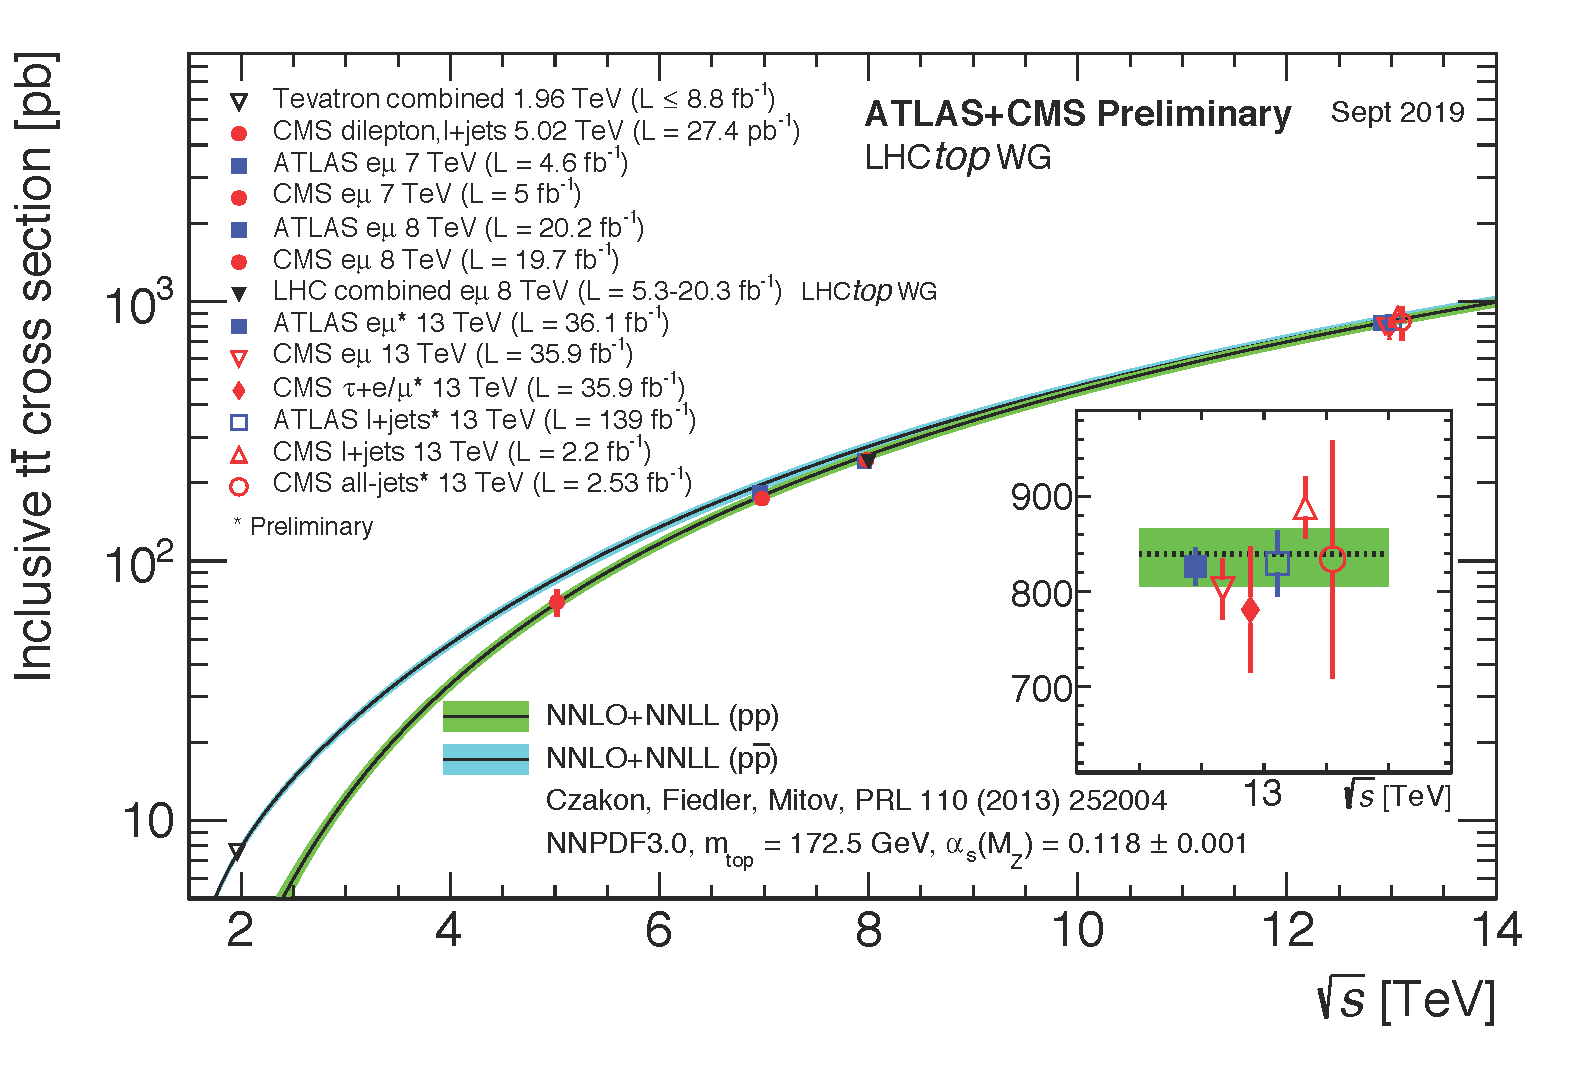
\includegraphics[width=\columnwidth]{../ThesisImages/Theory/ttprodxsec.png}
	\caption[Summary of $t\bar{t}$ production cross sections as a function of center of mass energy at Fermilab's Tevatron and CERN's LHC]{Summary of $t\bar{t}$ production cross sections as a function of center of mass energy at Fermilab's Tevatron and CERN's LHC.  For a top mass of 172.5 GeV and center of mass energy of 13 TeV the central value cross section is calculated to be 831 pb }
	\label{fig:ttbarXSec}
\end{figure}

\begin{figure}[h!]
	\centering
	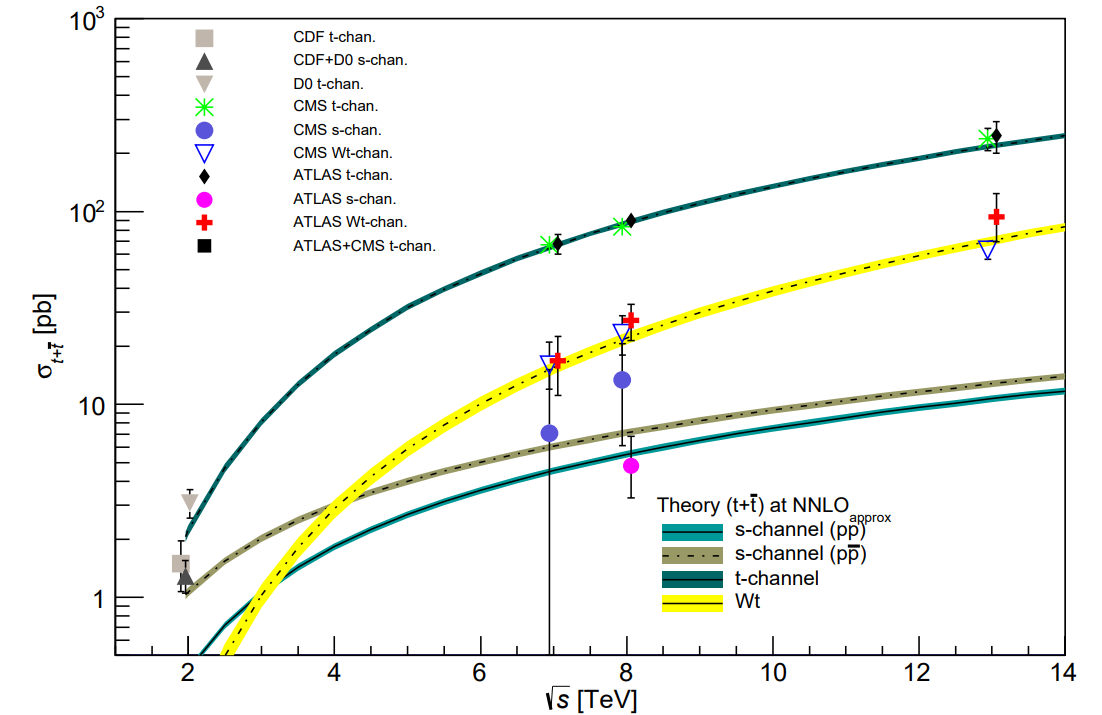
\includegraphics[width=\columnwidth]{../ThesisImages/Theory/singtprodxsec.png}
	\caption{Summary of single-top production cross sections as a function of center of mass energy at Fermilab's Tevatron and CERN's LHC.}
	\label{fig:singtXSec}
\end{figure}

 The amount of top quarks we produce scale up by the energy as seen in Figure \ref{fig:ttbarXSec} as well as the integrated luminosity, or number of events produced, of the accelerator and detector setup.  The LHC has significantly more of both than the Tevatron did.  Throughout the entirety of Run 2 at the LHC we expect there to be more than 115,000 top pair events produced within the ATLAS detector.  This will allow us to probe the details of the top quark better than ever before.  


\subsection{Production and Decay At Hadron Colliders}

There are multiple ways to produce top quarks at the LHC.  The most prevelant production mechanism of top quarks is through producing top/anti-top quark pairs.  This can be done, to leading order, either by quark-antiquark annihilation (Figure \ref{fig:LOprod}a) or gluon gluon fusion (Figure \ref{fig:LOprod}b-d).  At the Tevatron, a proton anti-proton collider the leading diagram was quark-antiquark annihilation because of the significantly larger amount of antiquarks in the collisions.  At the LHC the major production mechanism is gluon-gluon fusion, $\approx 90\%$, while quark-antiquark annihilation accounts for only $\approx 10\%$  of top quark pair production.  This is a strong interaction process and is therefore quite common, the cross sections are shown in Figure \ref{fig:ttbarXSec}.

\begin{figure}[h!]
	\centering
	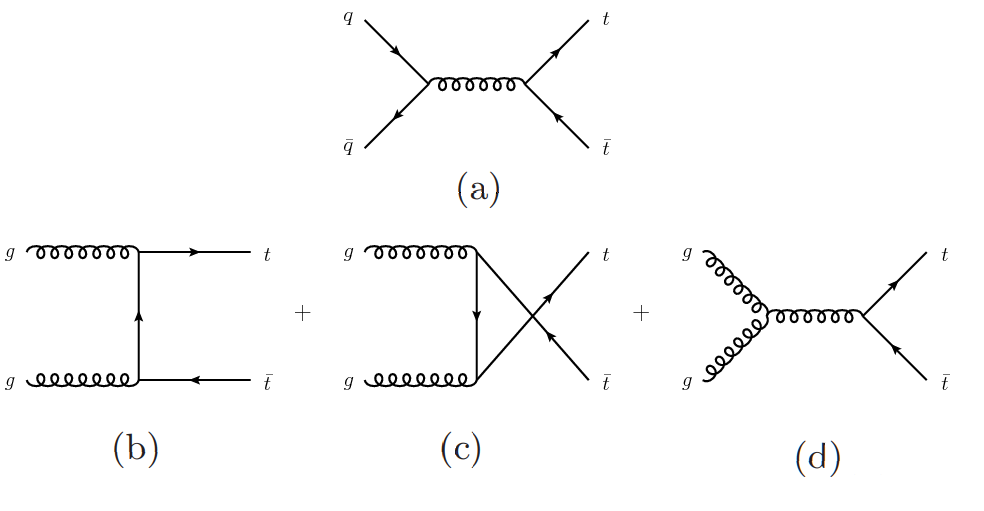
\includegraphics[width=\columnwidth]{../ThesisImages/Theory/LOPairProdDiags.png}
	\caption[Leading order diagrams for $t\bar{t}$ production at hadron colliders]{Leading order diagrams for the production of top/anti-top quark pairs at hadron colliders.  Quark-antiquark annihilation diagram in (a) while (b)-(d) show various gluon-gluon fusion diagrams}
	\label{fig:LOprod}
\end{figure}

Single top quarks can also be produced through weak interactions, which is less common and the leading diagrams are shown in Figure \ref{fig:LOprodSing} and their cross sections as measured at the LHC and Tevatron are shown in Figure \ref{fig:singtXSec}.  Comparing the leading production mechanisms at 13 TeV it can be seen that $t\bar{t}$ production is about a factor of 4 larger than single top production.  This means there are about 8x as many top quarks looking at pair produced events as you get two per event while giving you an additional experimental handle in looking for an invariant mass of final state products around the top quark mass.

\begin{figure}[h!]
	\centering
	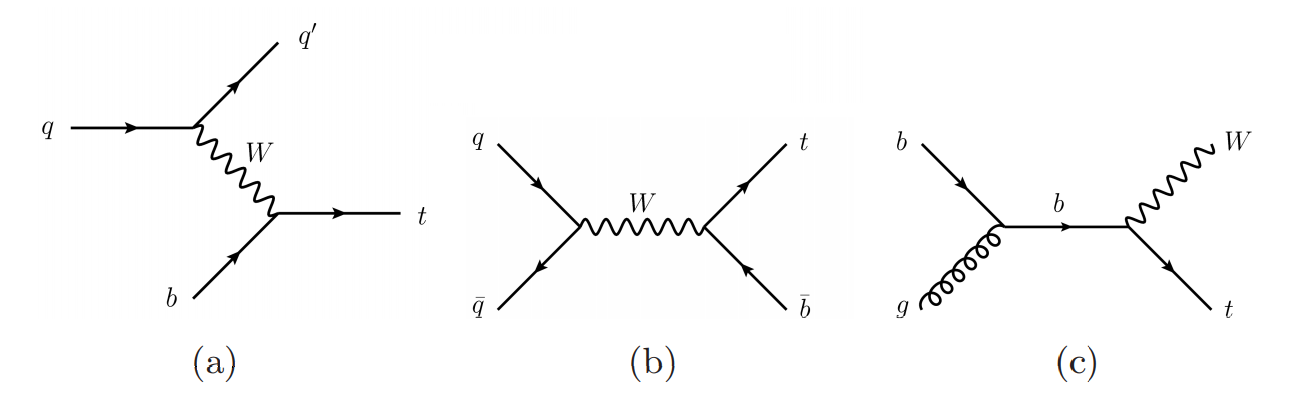
\includegraphics[width=\columnwidth]{../ThesisImages/Theory/LOSingProdDiags.png}
	\caption[Leading order diagrams for single top quark production]{Leading order diagrams for the production of single top quarks at hadron colliders.  The t-channel diagram is shown in (a), the s-channel in (b), and production in association with a W-boson is shown in (c)}
	\label{fig:LOprodSing}
\end{figure}

Since the top quark decays before hadronization we can study the branching ratios to various products directly.  Figure \ref{fig:SMDecays} shows various ways the top quark is allowed to decay in the standard model.  Figure \ref{fig:SMDecays}a shows the most likely decays where the top quark goes to a down-type quark and a W boson.  The branching ratio of these decays goes as the square of the corresponding matrix element in the CKM matrix as shown in Section \ref{sec:CKM}.  The sum of those branching ratios is unity within standard error bars such that the implication that the diagrams, corresponding to the flavor-changing neutral current decays, shown in Figure \ref{fig:SMDecays}b are highly supressed which will be explored further in Section \ref{sec:FCNC}.  


\begin{figure}[h!]
	\centering
	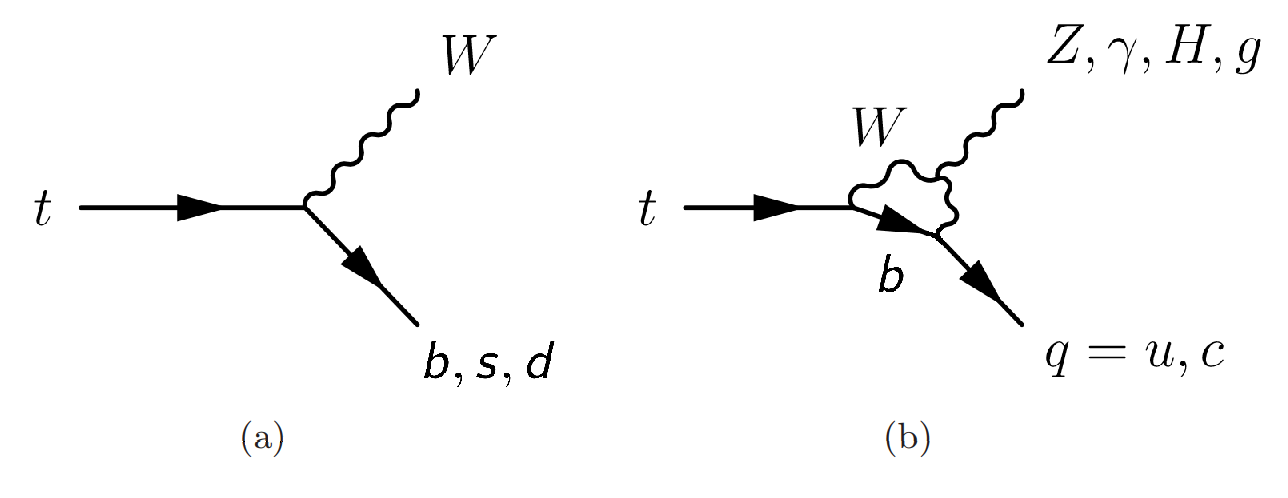
\includegraphics[width=\columnwidth]{../ThesisImages/Theory/SMTopDecays.png}
	\caption[Top quark decays in the Standard Model]{Top quark decays in the Standard Model.}
	\label{fig:SMDecays}
\end{figure}

Since the matrix element $V_{tb}$ in the CKM matrix is essentially unity each top usually decays to a b quark and a W boson.  The final state of the top pair events are then typically categorized by the decay of the W bosons.  The W boson can decay leptonically to a lepton (electron, muon, or tau) and its associated neutrino or hadronically to quarks.  This means top pair events are described as "all-hadronic" where both W bosons decay hadronically, "leptonic" if both W bosons decay leptonically, or "semi-leptonic" if one W boson decays hadronically and the other leptonically.  The ratios of these events is shown in Figure \ref{fig:ttdecayprods}.  However, because of how the tau decays and interacts these events are typically treated separately and only the electron and muons are considered as the leptons in the "semi-leptonic" final state of a $t\bar{t}$ event.  A quick counting (neglecting final state particle masses) of the final states of W bosons  is shown in Table \ref{tab:WFinals}.  The unitarity condition of the CKM matrix then implies that $|V_{ud}|^2 + |V_{us}|^2 + |V_{ub}|^2 =1$.  The phase space of the final product then has 1 state for each of the leptons and approximately 3 for each of the up type quarks so we expect a single top to decay into a lepton $\approx \frac{3}{9}$ of the time or any combination of quarks the other $\approx \frac{6}{9}$ of the time.  This holds when looking at the branching ratios of top quark pairs in Figure \ref{fig:ttdecayprods}.  The end result of this is that the regions of special interest for this dissertation, the electron and muon semi-leptonic final states occur $\approx 30\%$ of the time.  While this is not the largest selection of the final state branching ratios the presence of a lepton makes these final states easier to look for.

\begin{table}[]
\begin{center}
\begin{tabular}{|c|c|c|c|c|c|}
 \hline 
Decay Mode           			        & States   & Decay Mode                             &  States			   &     Decay Mode 		 	   &     States                          \\   \hline
$W^+ \rightarrow e^+ \nu_e$ 	        &1          &   $W^+ \rightarrow u\bar{d}$   &  $\times 3 |V_{ud}|^2$  &   $W^+ \rightarrow c\bar{d}$  &   $\times 3 |V_{cd}|^2$\\
$W^+ \rightarrow \mu^+ \nu_\mu$   &1          &  $W^+ \rightarrow u\bar{s}$    &  $\times 3 |V_{us}|^2$   &   $W^+ \rightarrow c\bar{s}$  &    $\times 3 |V_{cs}|^2$\\
$W^+ \rightarrow \tau^+ \nu_\tau$  &1	 &  $W^+ \rightarrow u\bar{b}$    &  $\times 3 |V_{ub}|^2$  &    $W^+ \rightarrow c\bar{b}$ &  $\times 3 |V_{cb}|^2$ \\ \hline
\end{tabular}
	\caption[Summary of final states of a W boson, when accounting for color permutations and the CKM matrix]{Summary of final states of a $W^+$ boson, when accounting for color permutations and the CKM matrix.  The table holds true if you flip all particles to their antiparticles}
	\label{tab:WFinals}
\end{center}
\end{table}

\begin{figure}[h!]
	\centering
	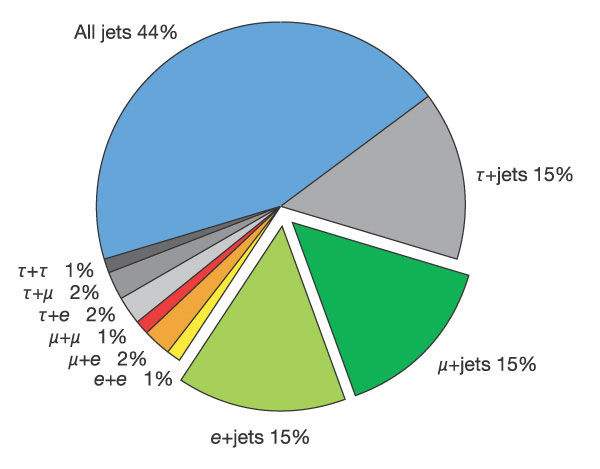
\includegraphics[width=.5\columnwidth]{../ThesisImages/Theory/topdecayproducts.jpg}
	\caption[Categorization of top quark pair decays in the Standard Model based on the decays of the W bosons]{Categorization of top quark pair decays in the Standard Model based on the decays of the W bosons.}
	\label{fig:ttdecayprods}
\end{figure}


\subsection{Beyond the Standard Model Top Quark Physics}

Many questions remain open with the intricacies of the Standard Model involving top quarks.  The mass of the top quark is at a mass scale similar to the W, Z, and Higgs bosons.  Does this imply the top plays a special role in the mechanism of electroweak symmetry breaking?  After the discovery of the Higgs: why do the top quark and Higgs boson have the exact masses they do which allows the electroweak potential to be stable up to very high energy scales as well as allowing the Universe to sit in a meta-stable state\cite{TopReview}.  The top quark is the main destabilizer of the Higgs potential because of its large mass it may be possible that new physics models will predict phenomena that can be more easily found in the properties of the top quark.  Many new physics models will present most dramatically in top quarks as radiative corrections to new massive particles will effect tops first before presenting in deviations in properties of the other, significantly lighter, fermions.  For example, a new Higgs like particle would most likely couple most strongly to the top quark.  
 Now that we have access to an unprecedented number of top quarks we can test the predictions of the Standard Model with much greater precision than ever before.  Top quark production modes, decay modes, couplings and various other properties are now being measured and providing limits on the phase spaces of any new physical models that exist or ruling out entire classes of models that have yet to be written down.  Arguably the properties of top quark are one of the most likely places that will point to a new understanding of our Universe.

 

\section{The Flavor-Changing Neutral Current}
\label{sec:FCNC}
  The idea of "flavor" in the Standard model refers to copies of the $SU(3)_C \times U(1)_{EM}$ representation as shown previously in Table \ref{tab:SMGaugePart}.  Specifically it will be used in the discussion in the generational change of one quark into another through some interaction.  For example, Figure \ref{fig:SMDecays}b shows a flavor-changing neutral current interaction.
\subsection{The Standard Model Flavor Sector}
Quarks that interact with $W^\pm$ bosons have interactinos that stem from the kinetic term of the Standard Model Lagrangian.  If we write this out explicitly in the mass eigenstates the interaction looks like:
\[ -\frac{g}{\sqrt{2}}\begin{pmatrix} \bar{u}_L & \bar{c}_L &\bar{t}_L \end{pmatrix} \gamma^\mu W_\mu^+ V\begin{pmatrix} d_L\\s_L\\b_L\end{pmatrix}+\text{h.c.}
\]
where the W interacts directly to change the flavor of quarks from an down(up)-type to an up(down)-type quark.  We can think of the CKM matrix as a rotation between the mass and interaction basis and the fact that the CKM matrix is non-diagonal means that the W boson interacts with quarks of different flavors.  The small off-diagonal elements of the CKM matrix mean that this generational change is a significantly smaller effect than interactions that change flavors within a generation, i.e. a top quark going to a bottom quark and W boson is much more likely than a top quark decaying to a down or strange quark and a W boson.  Going two generations away you get further from the diagonal and the mixing from the CKM matrix is even smaller.  The interaction with a W between two quarks is the only interaction vertex in the Standard model that allows for both flavor and generation changes.

As opposed to this flavor changing charged current interaction the flavor changing neutral current (FCNC) is an interaction between neutral gauge bosons and fermions.  These FCNC processes involve either up or down type quarks or involves charged or neutral leptons.  The flavor of the fermion is changed but the electric charge is conserved because it interacts with a neutral boson as opposed to the $W^\pm$ like in the charged current interaction.  FCNC interactions are forbidden at tree-level in the Standard model but can occur via higher order processes such as loops (as shown in Figure \ref{fig:SMDecays}b)

There are four neutral bosons in the Standard Model: the gluon, photon, Higgs boson, and Z boson.  Each of these can mediate FCNC interactions but all are forbidden at tree-level.  The gluon and photon correspond to exact gauge symmetries and have diagonal, flavor universal couplings since their interactions with fermions come through the kinetic terms.  The ramification of this is that they only interact with fermions of the same flavor.  The Standard Model Higgs cannot couple to fermions of different flavor since the Standard Model fermions are chiral and the Higgs couplings to fermions align with the fermion mass matrix.  In the Standard Model there is only a single Higgs doublet and the only source of the fermionic masses is the Higgs vacuum expectation value.  The Z boson can only connect to quarks from the same type (up or down).  When you move from the interaction to the mass eigenstates the rotation matricies only include terms such as $U_{uL}U_{uL}^\dagger = 1$ as opposed to the CKM matrix terms ($U_{uL}U_{dL}^\dagger$) which means these couplings are also flavor universal. 
The Standard Model FCNC suppression is built in though these means as opposed to generation-changing charged current processes.  The charged current processes rely on the CKM parameters which are free parameters of the Standard Model and as such they are measured and "put in".  These FCNCs are suppressed multiple ways in the Standard Model.

\subsection{The GIM Mechanism}
Historically the original Cabibbo model of particle physics only had three quarks; the up, down and strange.  Studies of Kaon decay during the late 1960's suggested there were no neutral current interactions in the Standard Model at the time.  The decay $K^+ \rightarrow \mu^+ \nu_\mu$ was observed but the process $K_L^0 \rightarrow \mu^+ \mu^- $ which was predicted was not observed.  Even in the absence of a tree level decay the $K_L^0$ decay the box diagram would be possible through the exchange of W bosons seen in Figure \ref{fig:KaonBox}.

\begin{figure}[h!]
	\centering
	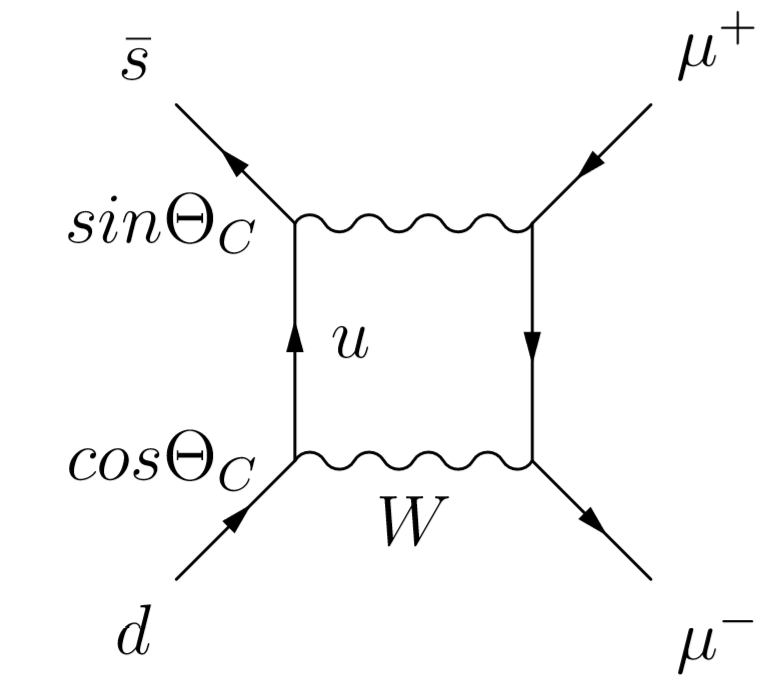
\includegraphics[width=.4\columnwidth]{../ThesisImages/Theory/GIMDiagramsa.png}
	\caption{Box diagram of $K_L^0 \rightarrow \mu^+ \mu^-$ through the exchange of W bosons.}
	\label{fig:KaonBox}
\end{figure}

Interactions at the time were thought to have strangeness quantum number interactions that changed strangeness in the following way:
\[ \Delta S=0 : u\bar{u} +d\bar{d}\text{cos}^2\Theta_C + s\bar{s} \text{sin}^2\Theta_C \]\[
\Delta S =1: (s\bar{d} + d\bar{s})\text{sin}\Theta_C \text{cos}\Theta_C  \]

The non-observation of the predicted decay led Glashow, Iliopoulous, and Maiani to predict the existence of a fourth quark, the charm, in 1970\cite{GIM}.  The addition of the charm led to two quak doublets and an almost perfect cancellation between the box diagrams:

\begin{figure}[h!]
	\centering
	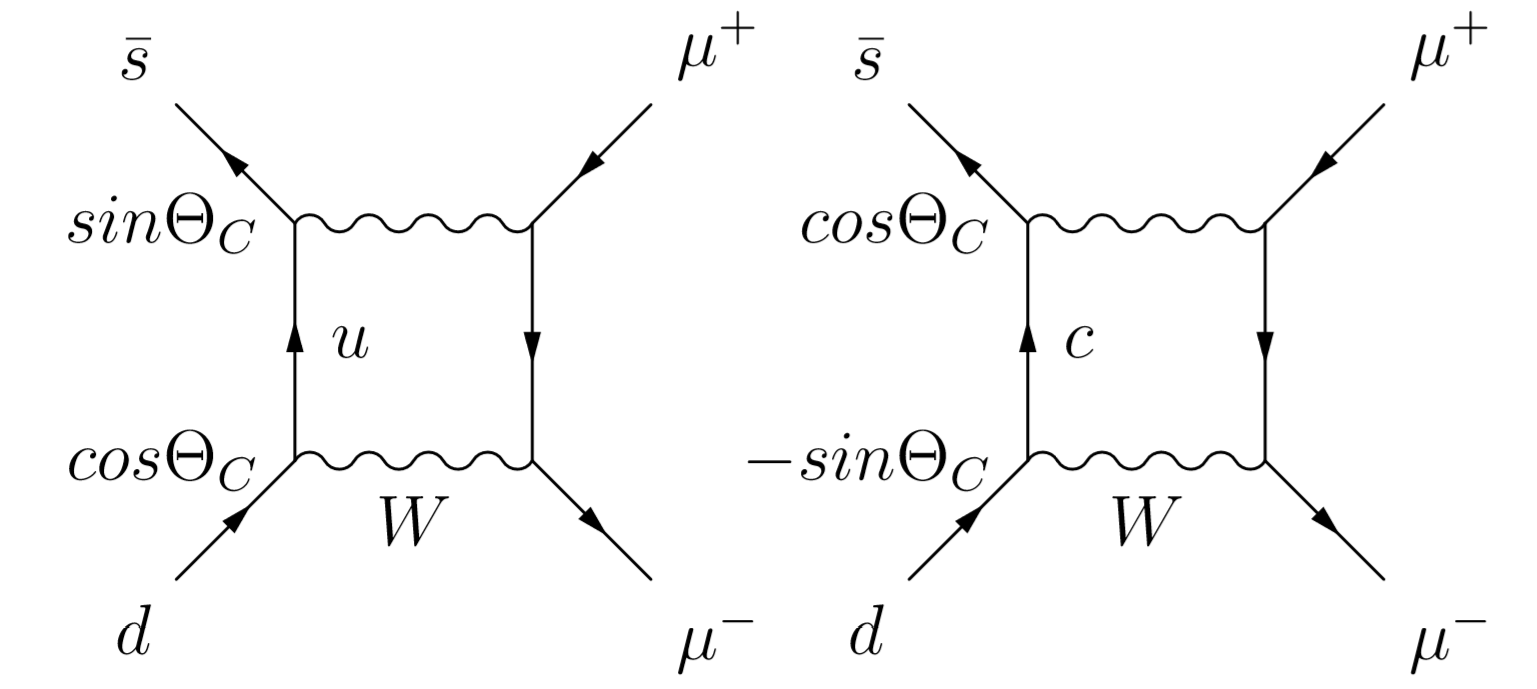
\includegraphics[width=.9\columnwidth]{../ThesisImages/Theory/GIMDiagrams.png}
	\caption{Box diagrams of $K_L^0 \rightarrow \mu^+ \mu^-$ through the exchange of W bosons after the inclusion of the charm quark.}
	\label{fig:KaonBox2}
\end{figure}

These box diagrams mean that we can rewrite strangeness change in interactions as 
\[ \Delta S=0 : u\bar{u} + c\bar{c} +(d\bar{d}+s\bar{s})\text{cos}^2\Theta_C + (s\bar{s}+d\bar{d}) \text{sin}^2\Theta_C \]\[
\Delta S =1: (s\bar{d} + d\bar{s} -d\bar{s}-s\bar{d})\text{sin}\Theta_C \text{cos}\Theta_C  \]

The addition of the charm means that, in the approximation $m_c = m_u$, the $\Delta S =1$ terms cancel exactly, the new box diagrams can be seen in Figure \ref{fig:KaonBox2}.  The FCNC interactions in top quark decays are suppressed through this mechanism as well, with the further inclusion of the bottom and top quarks.  They are further suppressed by being proportional to the quark mixing of off-diagonal elements in the CKM matrix, which are significantly less than 1.  A loop diagram for top quark FCNC is shown in Figure \ref{fig:FCNCLoop}.  This loop process is very rare.  The Standard Model branching ratio for these top FCNC interactions are shown along predicted enhancements from a variety of models of physics beyond the Standard Model in Table \ref{tab:FCNCLimits}.

\begin{figure}[h!]
	\centering
	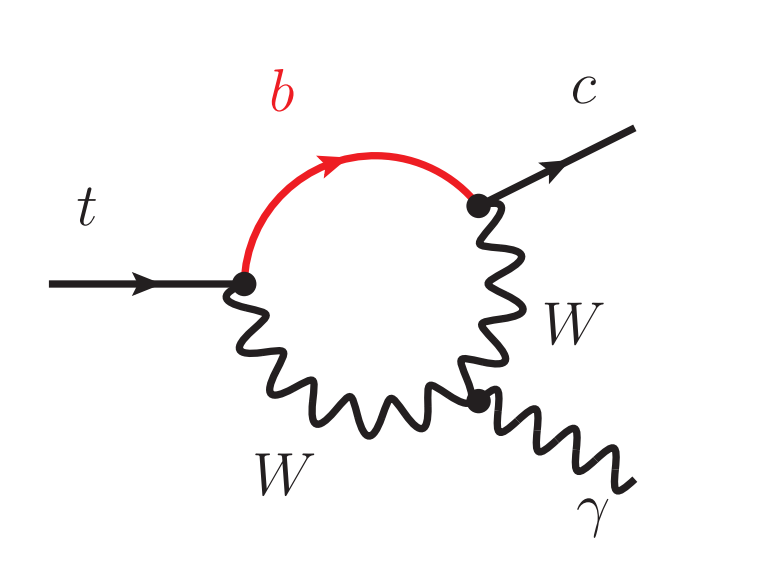
\includegraphics[width=.5\columnwidth]{../ThesisImages/Theory/FCNCLoop.png}
	\caption{An example loop diagram of a top quark decaying to a light quark and a photon.}
	\label{fig:FCNCLoop}
\end{figure}


\begin{table}[]
\begin{center}
\begin{tabular}{lllllll}
 \hhline{=======}
Process                                    & SM                        & 2HDM                   & QS                           & MSSM                   & RPV                          & XD                                 \\   \hline 
$t\rightarrow u\gamma $ &    $ 4*10^{-16} $        & $ -  $                   & $ \leq 4*10^{-8} $   & $ \leq 10^{-8} $ & $ \leq 10^{-9} $      &  $- $                                             \\
$t\rightarrow c\gamma $ &    $ 5*10^{-14} $        & $ \leq 10^{-7}   $ & $ \leq 4*10^{-8} $ & $ \leq 10^{-8} $ & $ \leq 10^{-9} $     & $ \leq 10^{-9}  $\\ \hline
$t\rightarrow u Z                    $ & $ 7*10^{-17} $  & $ -                     $ & $ \leq 6*10^{-4} $ & $ \leq 10^{-7} $ & $ \leq 10^{-6} $     & $ -  $                                             \\
$t\rightarrow c Z                    $ & $ 1*10^{-14} $  & $ \leq 10^{-6}   $ & $ \leq 6*10^{-4} $ & $ \leq 10^{-7} $ & $ \leq 10^{-6} $     & $ \leq 10^{-5} $ \\
$t\rightarrow u g                    $ & $ 4*10^{-14} $  & $ -                     $ & $ \leq 9*10^{-7} $ & $ \leq 10^{-7} $ & $ \leq 10^{-6} $     & $ -  $                                             \\
$t\rightarrow c g                    $ & $ 5*10^{-12} $  & $ \leq 10^{-4}   $  & $ \leq 9*10^{-7} $ & $ \leq 10^{-7} $ & $ \leq 10^{-6} $    & $ \leq 10^{-10} $ \\
$t\rightarrow u H                    $ & $ 2*10^{-17} $  & $ \leq 6*10^{-6} $ & $ -                      $ & $ \leq 10^{-5} $ & $ \leq 10^{-9} $     & $ -    $                                           \\
$t\rightarrow c H                    $ & $ 3*10^{-15} $  & $ \leq 2*10^{-3} $ & $ -                      $ & $ \leq 10^{-5} $ & $ \leq 10^{-9} $     & $ \leq 10^{-4} $ \\
\hhline{=======}
\end{tabular}
	\caption[Expected branching ratios for various flavor-changing neutral current processes in the Standard Model and multiple theories that predict enhancements to the branching ratio.  Two-Higgs Double Models with flavor-violating Yukawa couplings (2HDM), quark single models (QS), minimal supersymmetry models with 1TeV squarks and gluinos (MSSM), R-parity violating supersymmetry models (RPV), and extra-dimensional models (XD).]{Expected branching ratios for various flavor-changing neutral current processes in the Standard Model and multiple theories that predict enhancements to the branching ratio.  Two-Higgs Double Models with flavor-violating Yukawa couplings (2HDM) \cite{2HDM-2,2HDM-3}, quark single models (QS) \cite{QS-1,QS-2}, minimal supersymmetry models with 1TeV squarks and gluinos (MSSM) \cite{MSSM}, R-parity violating supersymmetry models (RPV) \cite{RPVSusyFCNC}, and extra-dimensional models (XD) \cite{XDFCNC}.}
	\label{tab:FCNCLimits}
\end{center}
\end{table}

\subsection{New Physics With Enhancements to FCNCs}
\label{sec:bsmFCNC}
Various theoretical models that include physics beyond what is included in the Standard Model are proposed to solve problems that exist with the Standard Model or an explanation of known phenomena that are not in agreement with the Standard Model.  Various models seek to solve different problems, e.g. providing a dark matter candidate or fixing the naturalness problem of the Standard Model resulting from an unexpectedly high amount of fine-tuning from loop corrections to the Higgs mass.  
Top quark FCNCs in the Standard Model are so currently so far from experimental reach ($\approx 10$ orders of magnitude) that they are impossible to observe even with major improvements to the accelerator and detector techonologies.  Table \ref{tab:FCNCLimits} also shows a variety of theories beyond the Standard Model which predict large enhancements to FCNC top couplings.  For the most part these enhancements come from terms that have very heavy particles moving in the loops.  Therefore searching for FCNCs with top quarks provides a particularly good handle to study models of new physics and rule out the phase spaces of these models by lowering the expected limit.  An explanation of the various models explored in Table \ref{tab:FCNCLimits} follows.

\textbf{Two-Higgs-Doublet Models (2HDM): } 2HDM are a simple extension of the SM which contain two Higgs doublets instead of the one currently contained in the Standard Model.  This leads to a much more rich phenomenology in the Higgs sector with two CP even neutral Higgs bosons ($h$ and a heavier $H$), a CP odd psudoscalar $A$ and two charged Higgs bosons $H^\pm$.  The currently discovered Higgs boson can be mapped to either h or H depending on various limits in the model of choice.  These models can typically be described by an additional six parameters: the four Higgs masses ($m_h, m_H,m_A,m_{H^\pm}$), the ratio of the two vacuum expectation values and a mixing angle that diagonalizes the mass matrix of the neutral CP even Higgs bosons.  Many Supersymmetric models predict the existence of an extra Higgs doublet.  Some of these models also attempt to explain the baryon asymmetry of the Universe\cite{Trodden:1998ym}.
2HDM Models predict very large enhancements to FCNC interactions due to an extension of the electroweak symmetry breaking sectors.  Some of these models (type III 2HDM, and models of minimal flavor violation) include tree level FCNCs\cite{Branco:2011iw} which is why the enhancement brings the branching ratio up to an observable level.

\textbf{Quark Singlet Models (QS): } QS involve an extension to the Standard Model in the form of an extra vector-like quark singlet that couples strongly to the top quark, typically in the form of a top-partner quark.  These heavier $t'$ quarks could explain the fine-tuning of the Higgs boson mass through cancelation of some or all of the top loop diagrams present in the radiative corrections to the Higgs mass.  These models generally imply then that the CKM matrix is no longer unitary and tree level FCNCs are then allowed which offers a great enhancement to potential branching ratios\cite{QS-1,QS-2}.

\textbf{Minimal Supersymmetric Models (MSSM): }  Supersymmetric Models were every Standard Model particle has a super particle partner typically aim to solve multiple problems with the Standard Model at once.  This is generally the fact that the lightest supersymmetric particle, which is stable, provides a good dark matter candidate.  MSSM models have super partner quarks (squarks) and super partner gluons (gluinos) on a mass scale of $\approx 1 \text{ TeV}$.  Top FCNCs can then occur through loop diagrams still, as they do in the Standard Model, but the loop is enhanced as it includes the supersymmetric particle of the top quark (the heavier stop quark)\cite{MSSM, MSSM-2}.

\textbf{R-Parity Violating Supersymmetric Models (RPV): }  Another supersymmetric model where R parity ($P_R = (-1)^{3 B + L +2 s}$), where B is baryon number, L is lepton number, and s is spin is no longer conserved.  FCNCs can also occur at the one loop level in these models in loops which no longer conserve baryon or lepton number.\cite{RPVSusyFCNC}

\textbf{Extra-dimensional Models (XD): }  XD Models are Randall-Sundrum models that describe the Universe as a warped-geometry higher dimensional space where elementary particles are localized on a (3+1)-dimensional brane.  These models offer a potential solution to the hierarchy problem of the Standard Model by adding in a mechanism to explain the difference between the typicaly scales over which FCNCs take place (the electroweak scale) and the Planck scale.  In these models FCNCs exist due to flavor-violating couplings between Standard Model fermions and Kaluza-Klein excitations of the gauge bosons in the Standard Model\cite{XDFCNC}.  Due to their overlap with Kaluza-Klein guage modes The flavor-violating couplings will be largest in the top sector.


\subsection{Current Measurements of Top FCNCs}

All four the neutral boson mediated FCNC channelss can be searched for individually and model independentally.  Each channel will have its own signature and various advantages and disadvantages in preforming the search.  Each of the potential tree-level diagrams is shown in Figure \ref{fig:AllFCNCs}, all of which are forbidden in the Standard Model.  Searching in the production of single top quarks %%%%%%%%%%%%%%%%
\begin{figure}[h!]
	\centering
	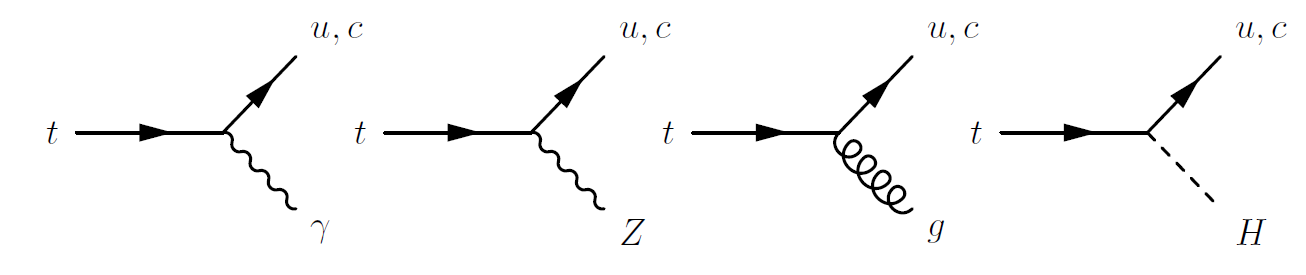
\includegraphics[width=\columnwidth]{../ThesisImages/Theory/AllFCNCDiagrams.png}
	\caption{Flavor-changing neutral current top quark decays.}
	\label{fig:AllFCNCs}
\end{figure}

The channels involving the all of the various neutral bosns can be serached for with the ATLAS detector in both single-top production modes as well as the decay mode through $t\bar{t}$ events.  All of the production channels provide a sharp separation between $u\rightarrow tX$ and $c\rightarrow tX$ but have fewer statistics than decays in the decay mode using $t\bar{t}$ events.  Some final states of these variouos FCNC events such as those involving the decay mode search for $t\rightarrow q Z$ can explot a tri-lepton final state ($Z\rightarrow ll$, with the other top decaying leptonically$t\rightarrow bW\rightarrow bl\nu$).  The process that involves the Higgs boson has the advantage of looking at a wide range of potential final states of the Higgs and can be successfully tackled using different methods.

\begin{figure}[h!]
	\centering
	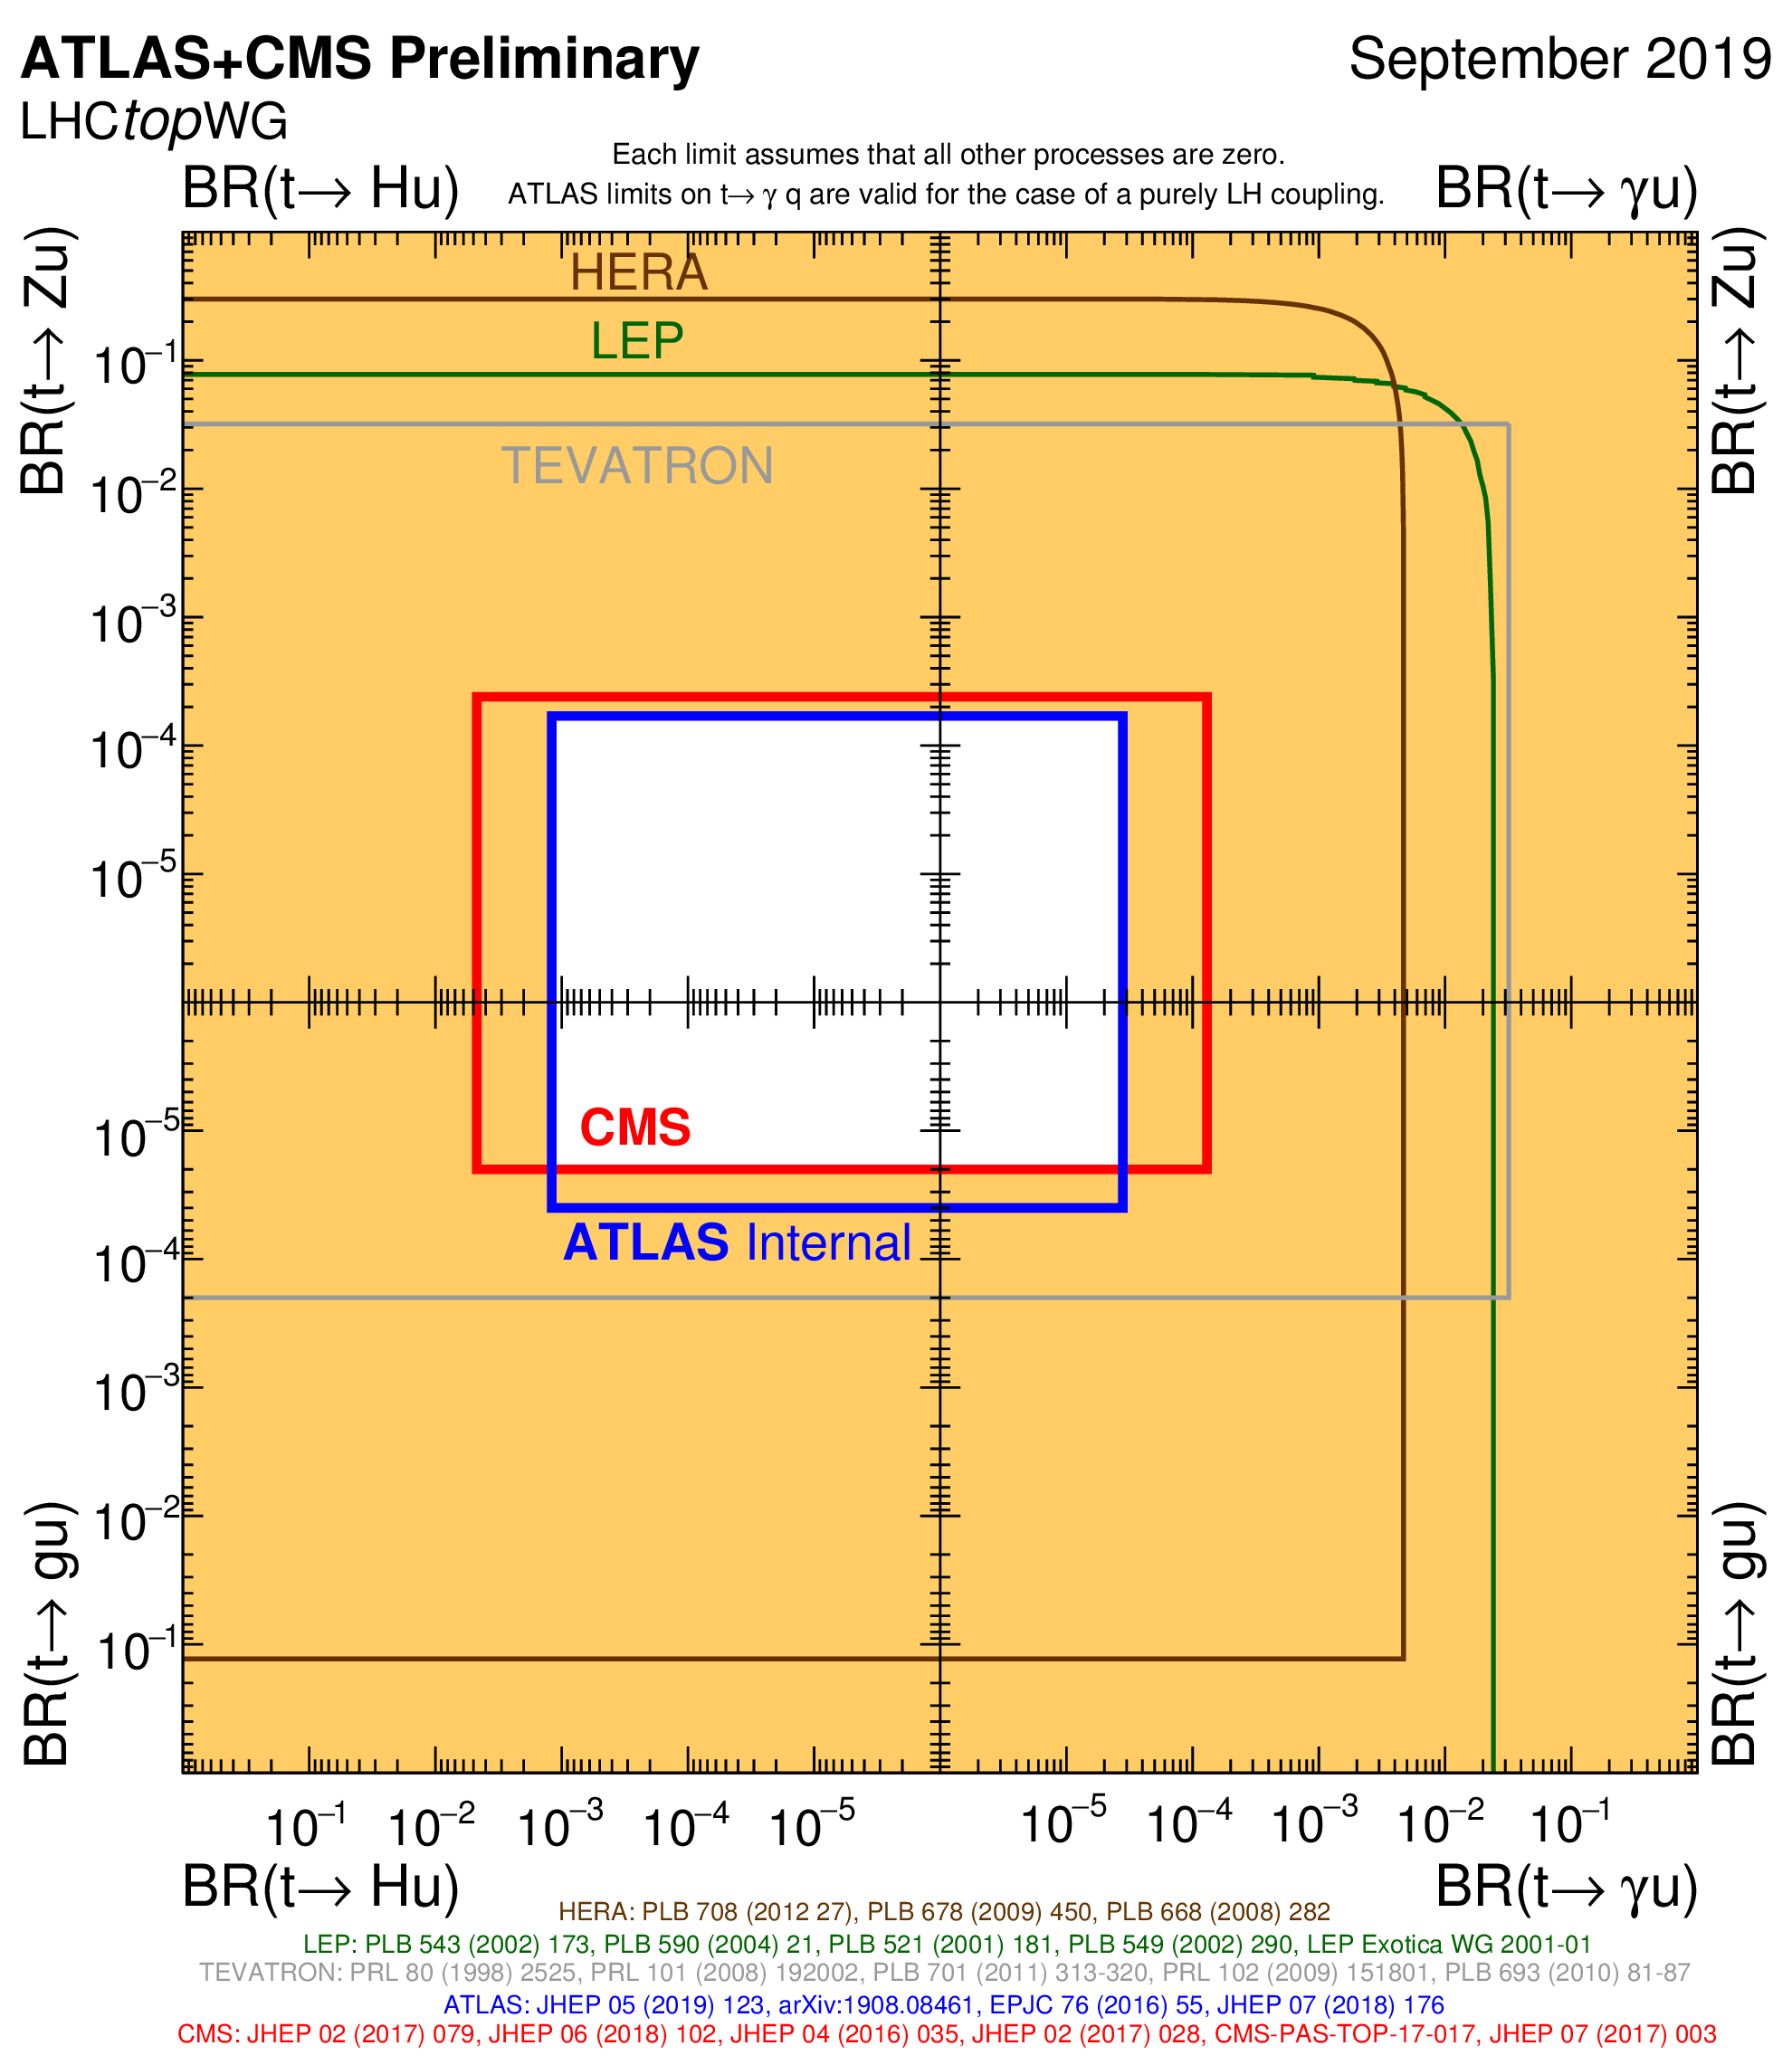
\includegraphics[width=.5\columnwidth]{../ThesisImages/Theory/fcnc_tXu_sep18.png}
	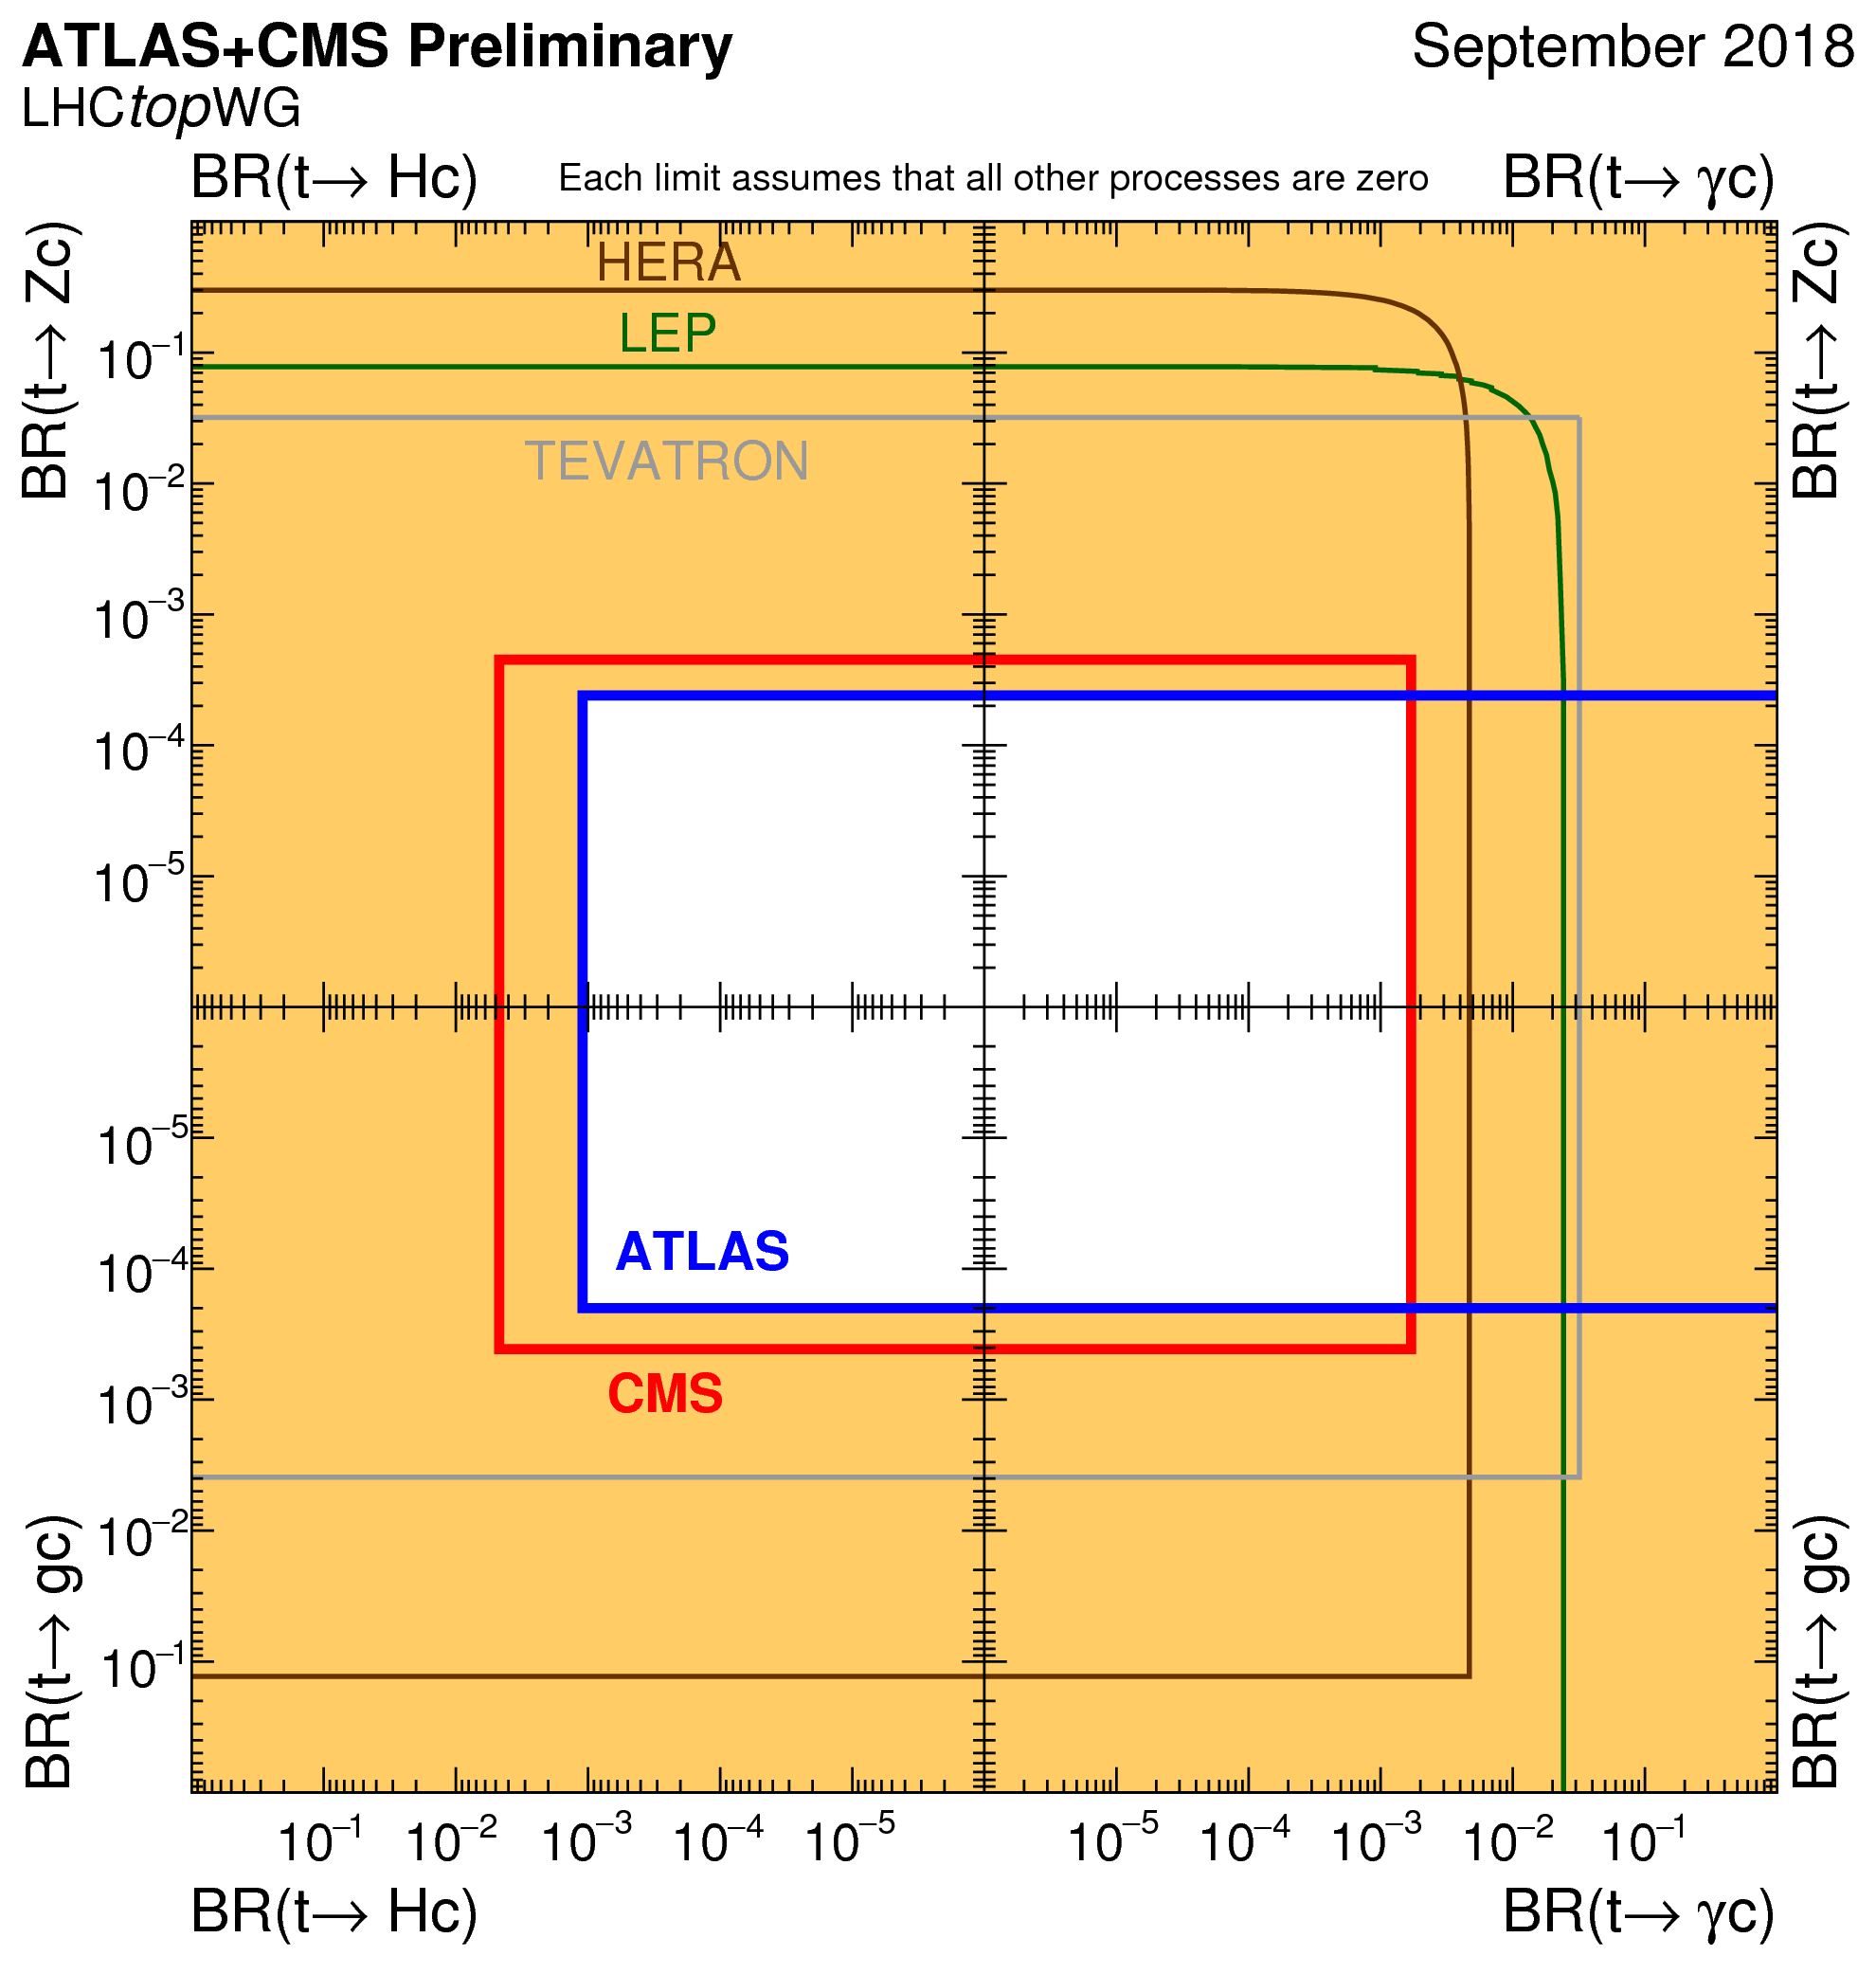
\includegraphics[width=.5\columnwidth]{../ThesisImages/Theory/fcnc_tXc_sep18.png}
	\caption{Flavor-changing limits from a variety of expeiments in every channel $t\rightarrow uX$(top) and $r\rightarrow cX$(bottom).}
	\label{fig:FCNCLimsBox}
\end{figure}

Limits have been set on these FCNC processes at various expierments in the past.  The electron-prodon collider HERA at DESY, the electron-proton collider LEP at CERN, and the proton-proton colliders the Tevatron at Fermilab and the LHC at CERN have all had experiments searching for the FCNC proccesses.  The collected limits of these experiments are shown in Figure \ref{fig:FCNCLimsBox}.  Due to the energy of these early colliders 209 GeV center of mass energy for LEP and 318 GeV for HERA only production modes could be searched for as they are below the production threshold for $t\bar{t}$ pairs. The diagrams looked for at these experiments are shown in Figure \ref{fig:fcncHera} (HERA) and Figure \ref{fig:fcncLep} (LEP).
\begin{figure}[h!]
	\centering
	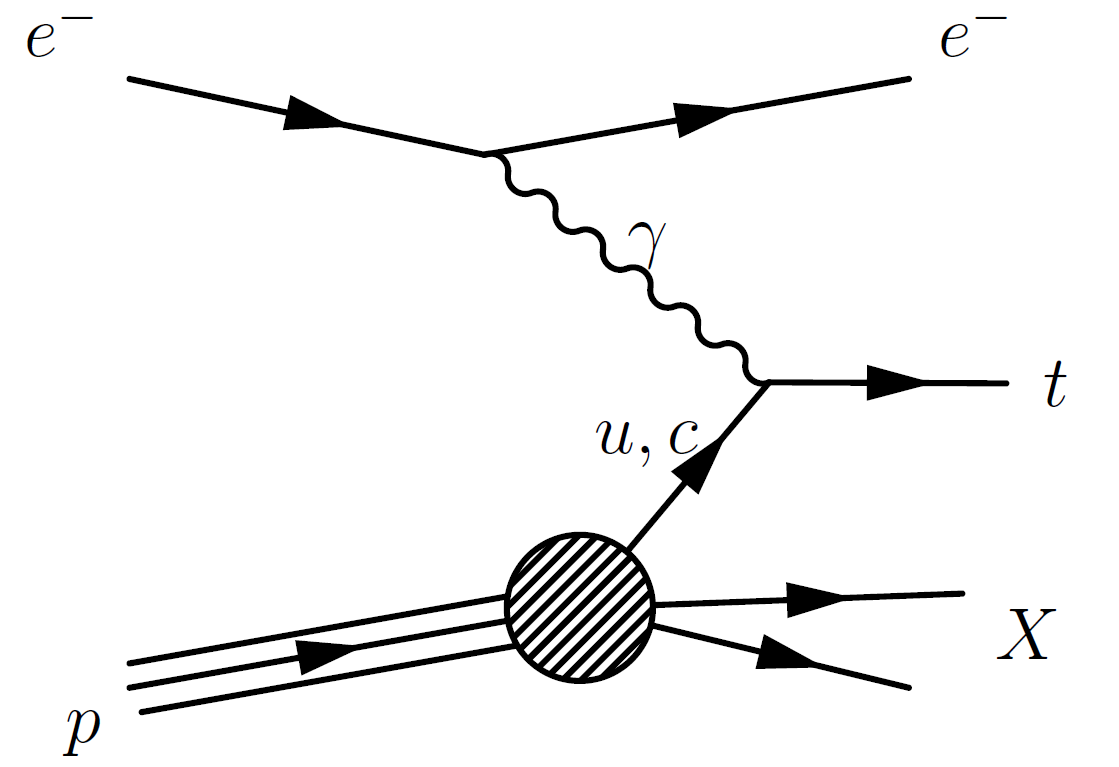
\includegraphics[width=.4\columnwidth]{../ThesisImages/Theory/HeraFCNC.png}
	\caption{FCNC diagram for the search in single top production at the electron-proton collider HERA.}
	\label{fig:fcncHera}
\end{figure}
\begin{figure}[h!]
	\centering
	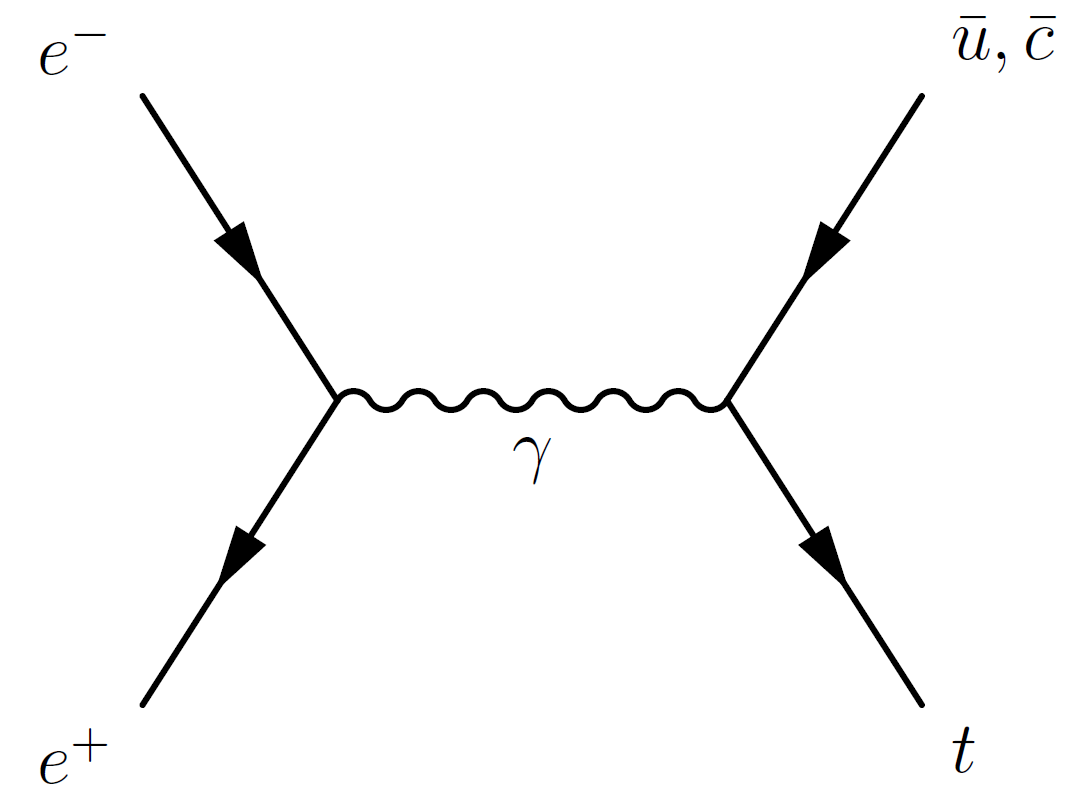
\includegraphics[width=.4\columnwidth]{../ThesisImages/Theory/LepFCNC.png}
	\caption{FCNC diagram for the search in single top production at the electron-positron collider, LEP.}
	\label{fig:fcncLep}
\end{figure}

Shown in Figure \ref{fig:FCNClimits} are the Standard Model theoretical predictions, various beyond the Standard model predictions (as discussed in Section \ref{sec:bsmFCNC}), and experimental limits for all processes $t\rightarrow Xq$ where q is an up-type quark and X is any neutral boson.  
\begin{figure}[h!]
	\centering
	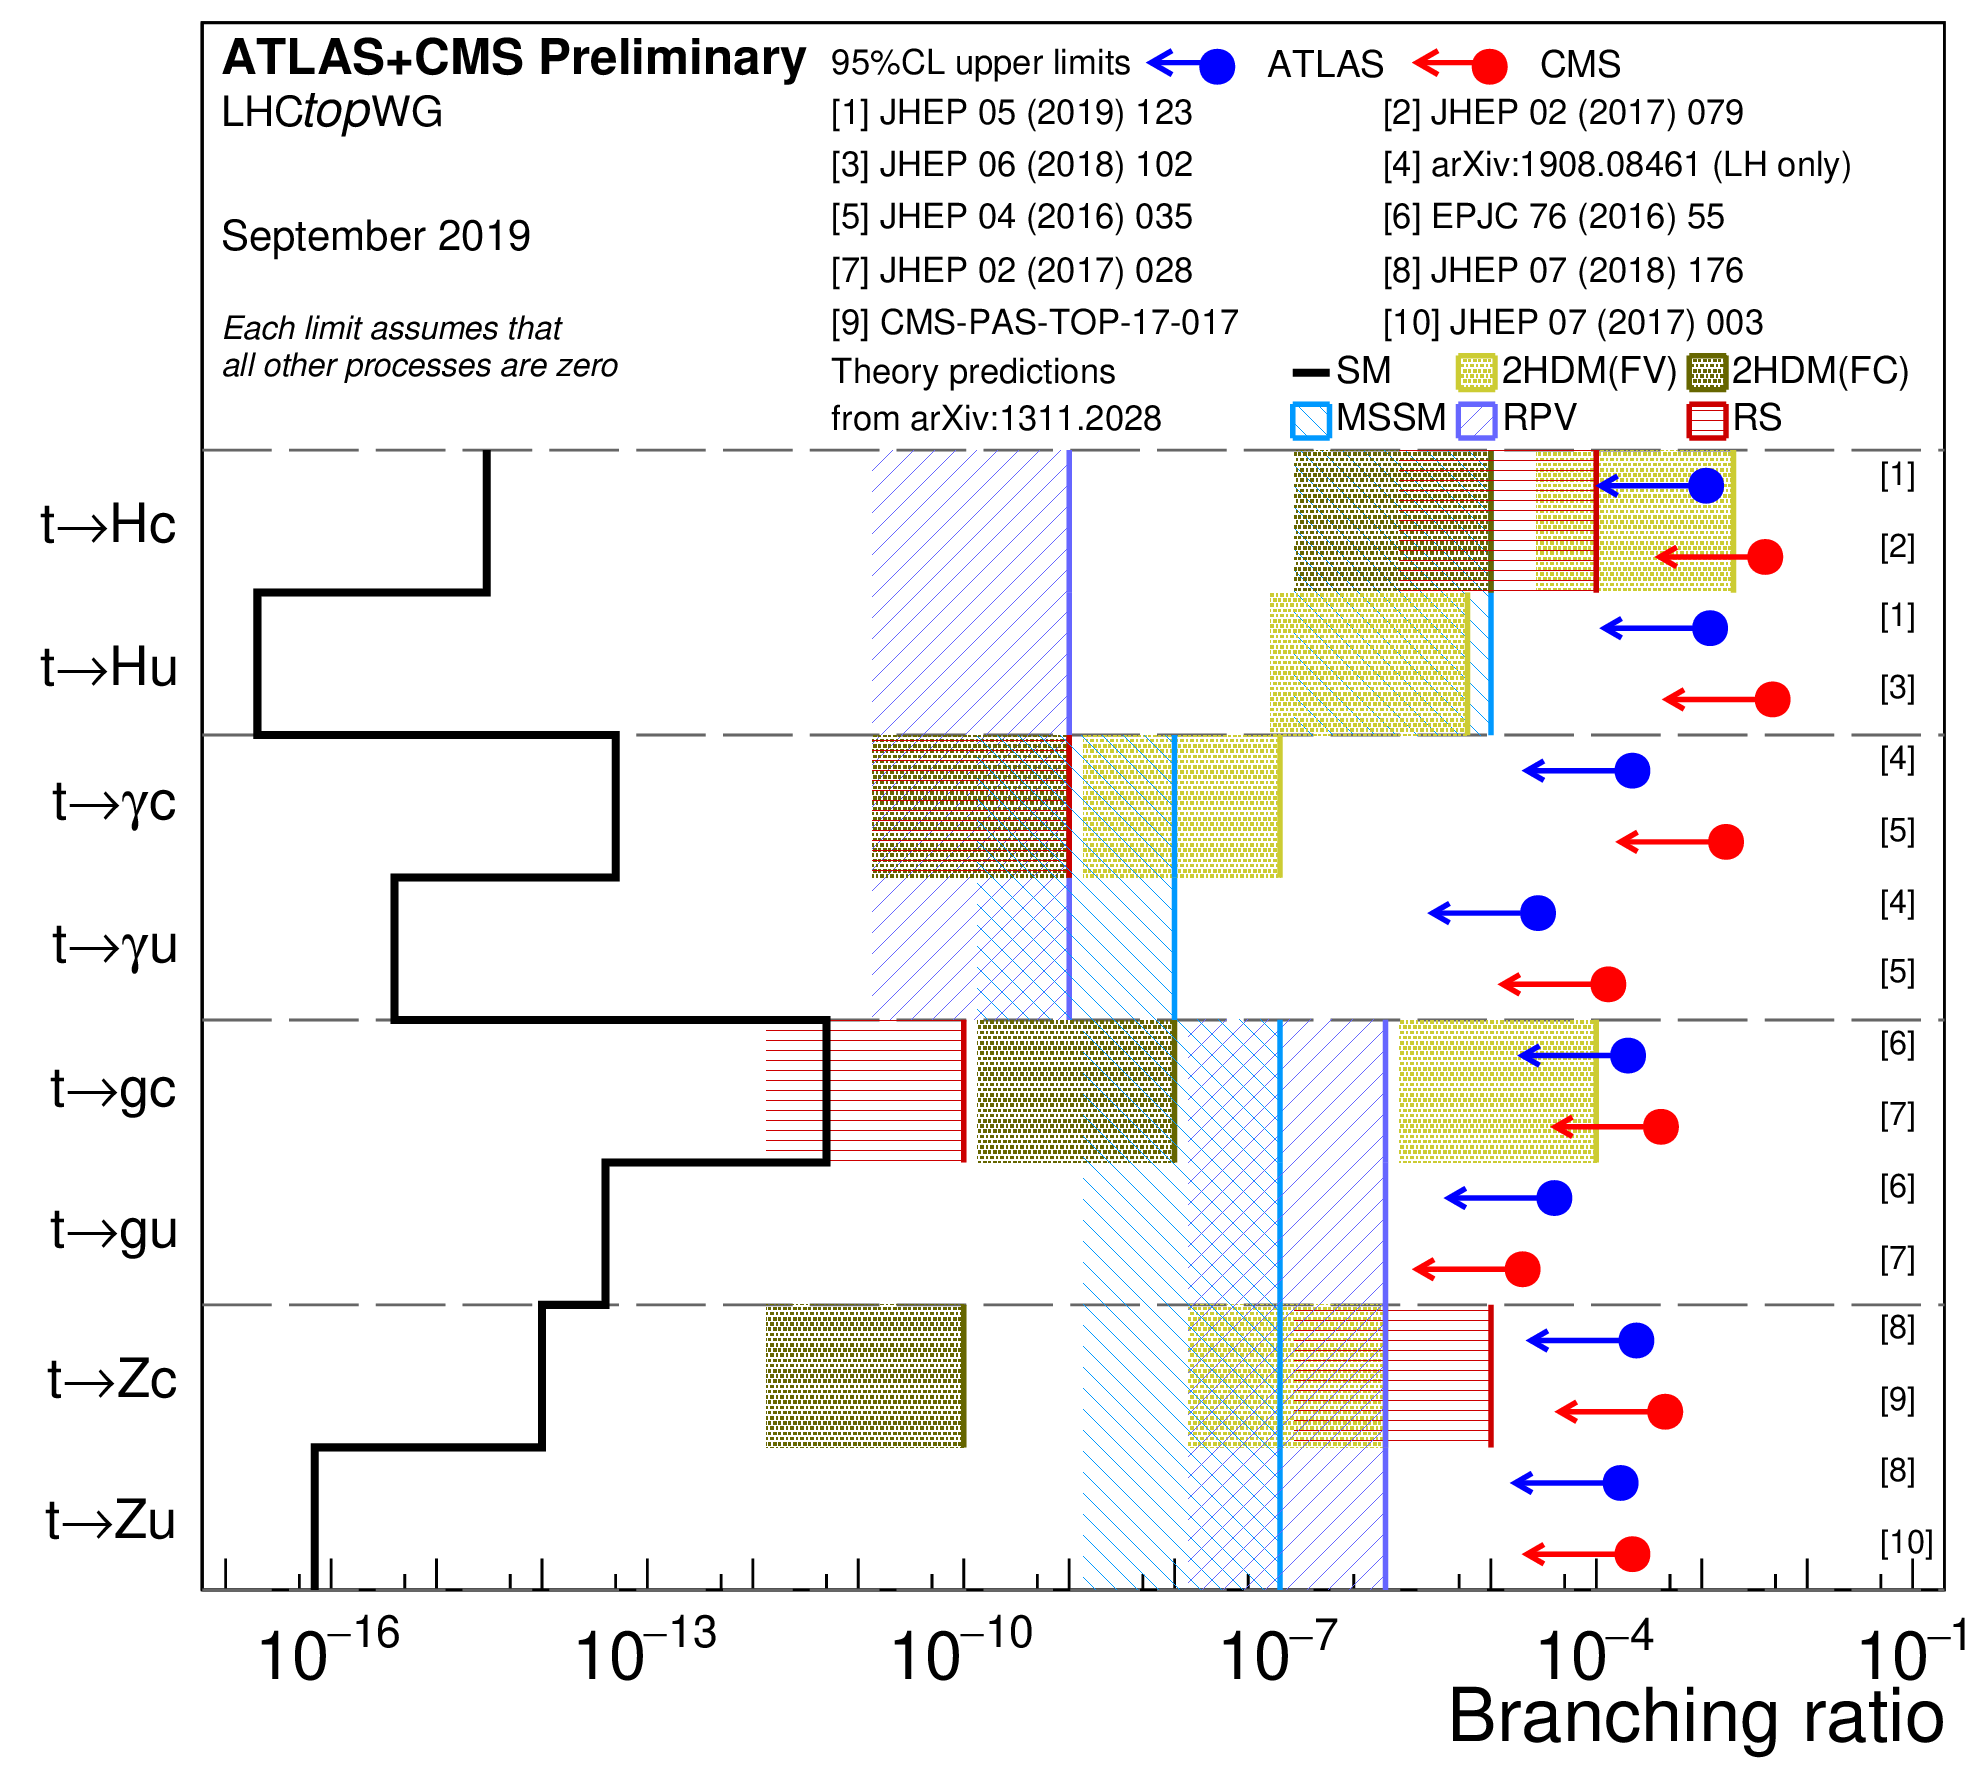
\includegraphics[width=.9\columnwidth]{../ThesisImages/Theory/AllFCNCLimits.png}
	\caption{Flavor-changing neutral current theoretical branching ratios and experimental limits (both ATLAS and CMS) updated through 2018.}
	\label{fig:FCNClimits}
\end{figure}

Since the publication of Figure \ref{fig:FCNClimits} the ATLAS experiment has published a result in the production mode of the $t\rightarrow q\gamma$ vertex using 81 $\text{fb}^{-1}$ of data (LHC data runs between 2015-2017).  Upper limits have been set on $t\rightarrow u \gamma$ left-handed (right-handed) branching ratio of $2.8\times 10^{-5}$ ($6.1\times 10^{-5}$) and upper limits on $t \rightarrow c \gamma$ left-handed (right-handed) branching ratio of $22\times10^{-5}$ ($18\times10^{-5}$) \cite{GregorFCNC}.  Production mode searches offer better reach for $t\rightarrow u \gamma$ over $t\rightarrow c \gamma$ due to the higher prevelance of up quarks in the parton distribution function of the colliding protons.

This dissertation presents a complementary search for the process $t\rightarrow q \gamma$ to the ATLAS single top production search in the decay channel using top quark pair events.  The process $t\bar{t} \rightarrow bWq\gamma \rightarrow bl\nu q\gamma$ will be searched for using the ATLAS detector.  This final state ($b l \nu q \gamma$) is a straightforward channel in that it has one of each type of object that can be reconstructed with ATLAS.  There are 2 jets from the quarks but one is a b-jet that has qualities that can distinguish it from a normal quark jet which will be discussed in Section \ref{sec:bjetReco}.  In addition to the jets the final state also has a charged lepton (here we will look in the electron and muon channels), a photon, and a neutrino.  The reconstruction of these objects is discussed in Chapter \ref{ch:Simulation}.  The FCNC process is a unique process where a top quark decays directly into an up-type quark and a photon we can require that the jet and photon we measure can be reconstructed into a top quark by making a mass requirement which gives an excellent handle for separating signal and background.






%
%CKM Matrix\cite{PDG2018}:
%\[
%\begin{pmatrix}
%d' \\ s' \\ b'
%\end{pmatrix}
%=
%\begin{pmatrix}
%V_{ud} & V_{us} & V_{ub} \\
%V_{cd} & V_{cs} & V_{cb} \\
%V_{td} & V_{ts} & V_{tb} 
%\end{pmatrix}
%= 
%\begin{pmatrix}
%d \\ s \\ b
%\end{pmatrix}
%\]

%
%%%%%%%%%%%%%%%%%%%%%%%%%%%%%%%%%%%%%%%%%%%%%%%
%%%%%%%%%%%%                                                                                                   %%%%%%%% 
%%%%%%%%%%%%                           BEN                                                                  %%%%%%%% 
%%%%%%%%%%%%                                                                                                   %%%%%%%% 
%%%%%%%%%%%%%%%%%%%%%%%%%%%%%%%%%%%%%%%%%%%%%%%

%\begin{figure}[]
%	\centering
%	\subfloat[]{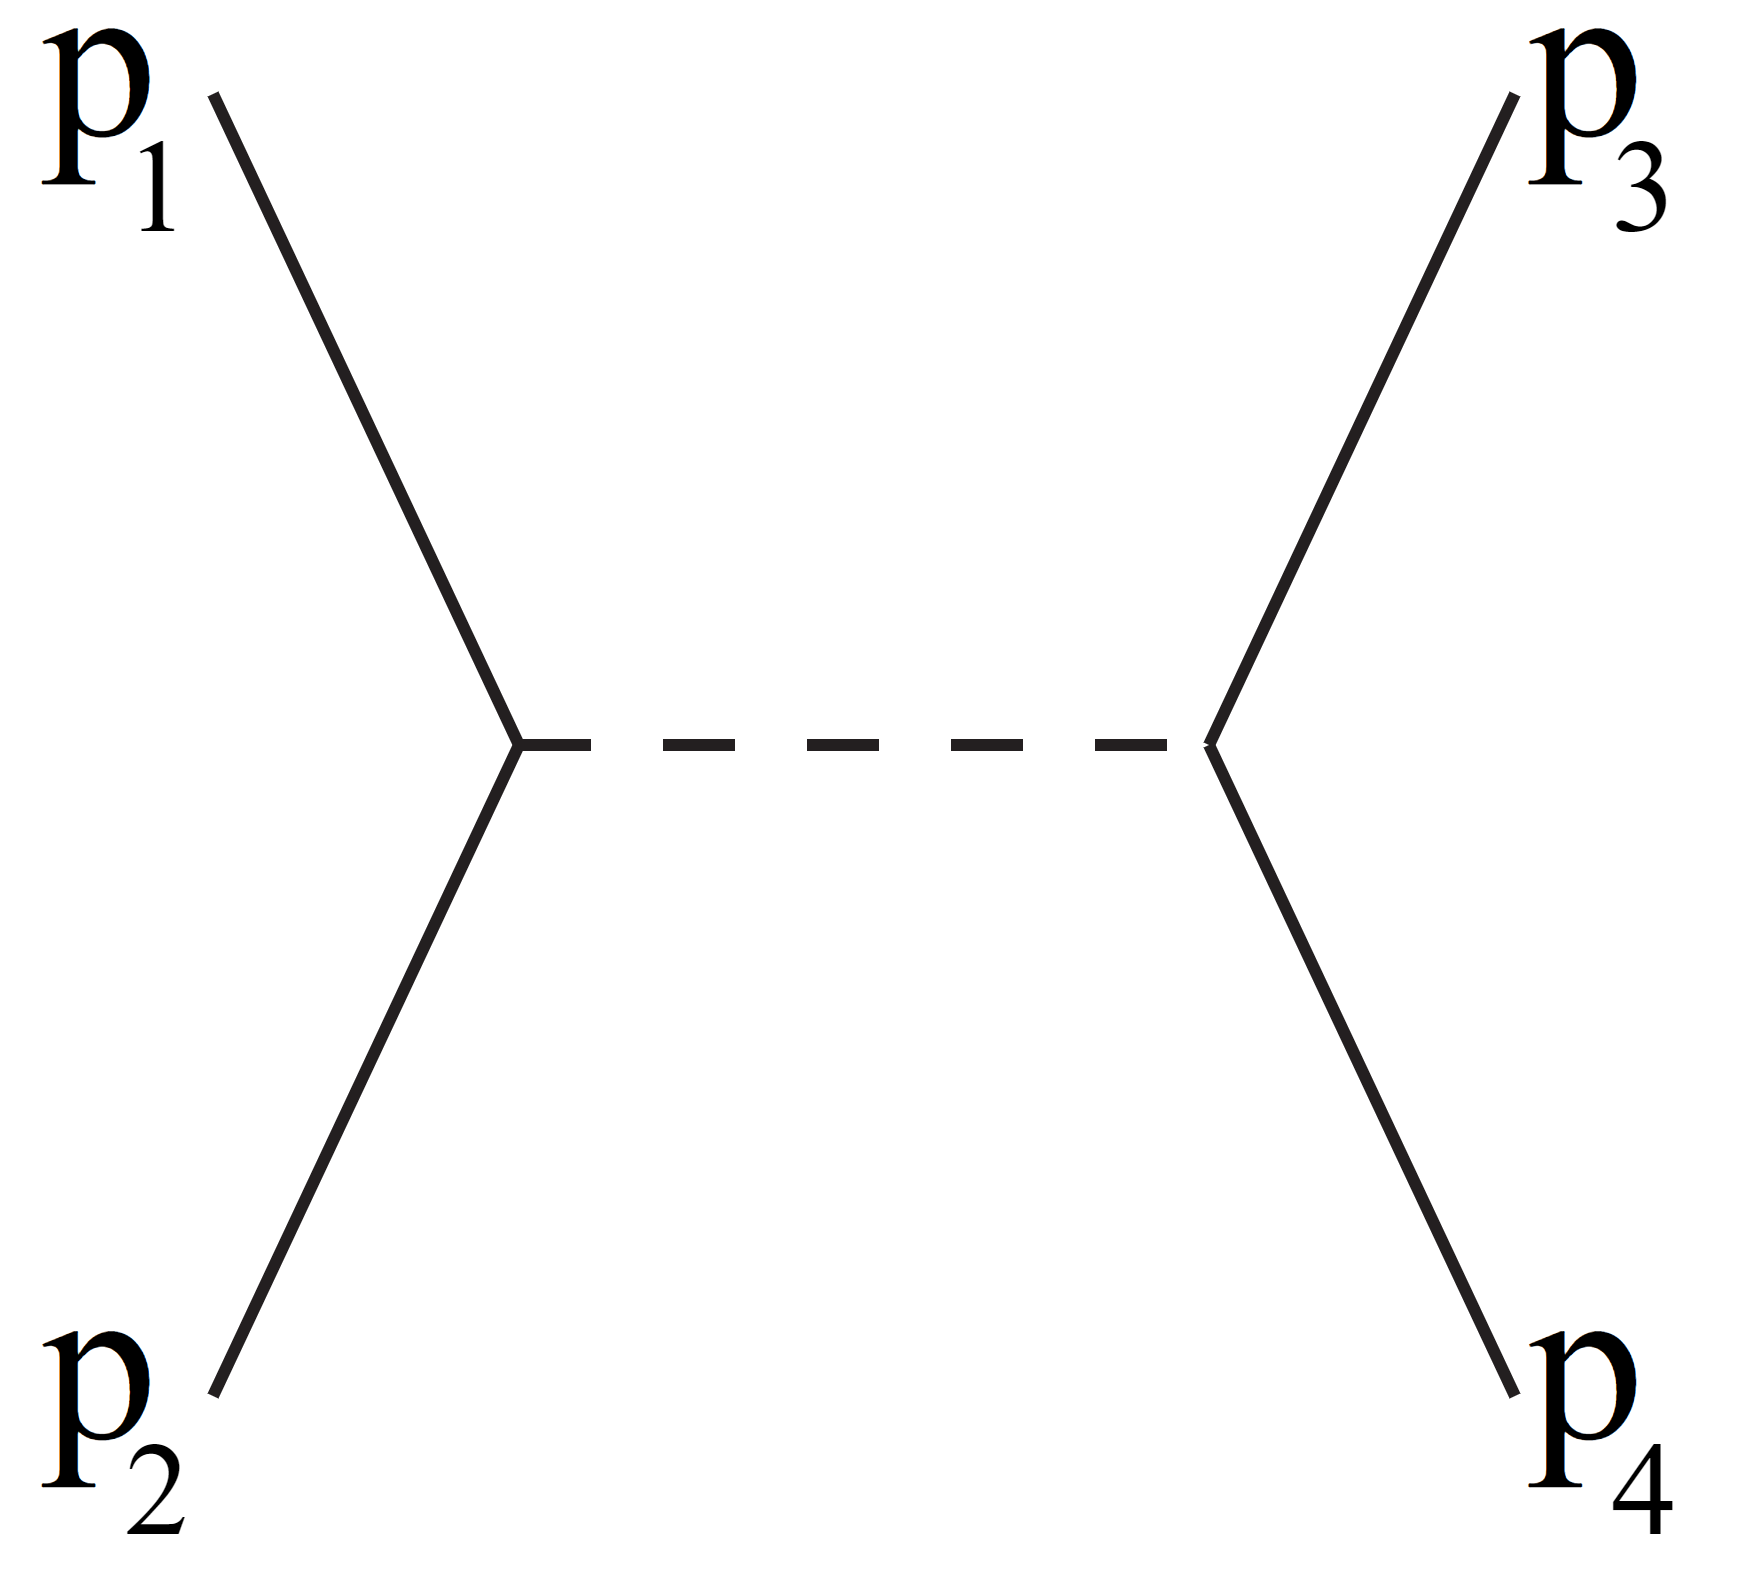
\includegraphics[width=0.35\columnwidth]{figures/Theory/SChannel.png}}
%	\hspace{0.1\columnwidth}%
%	\subfloat[]{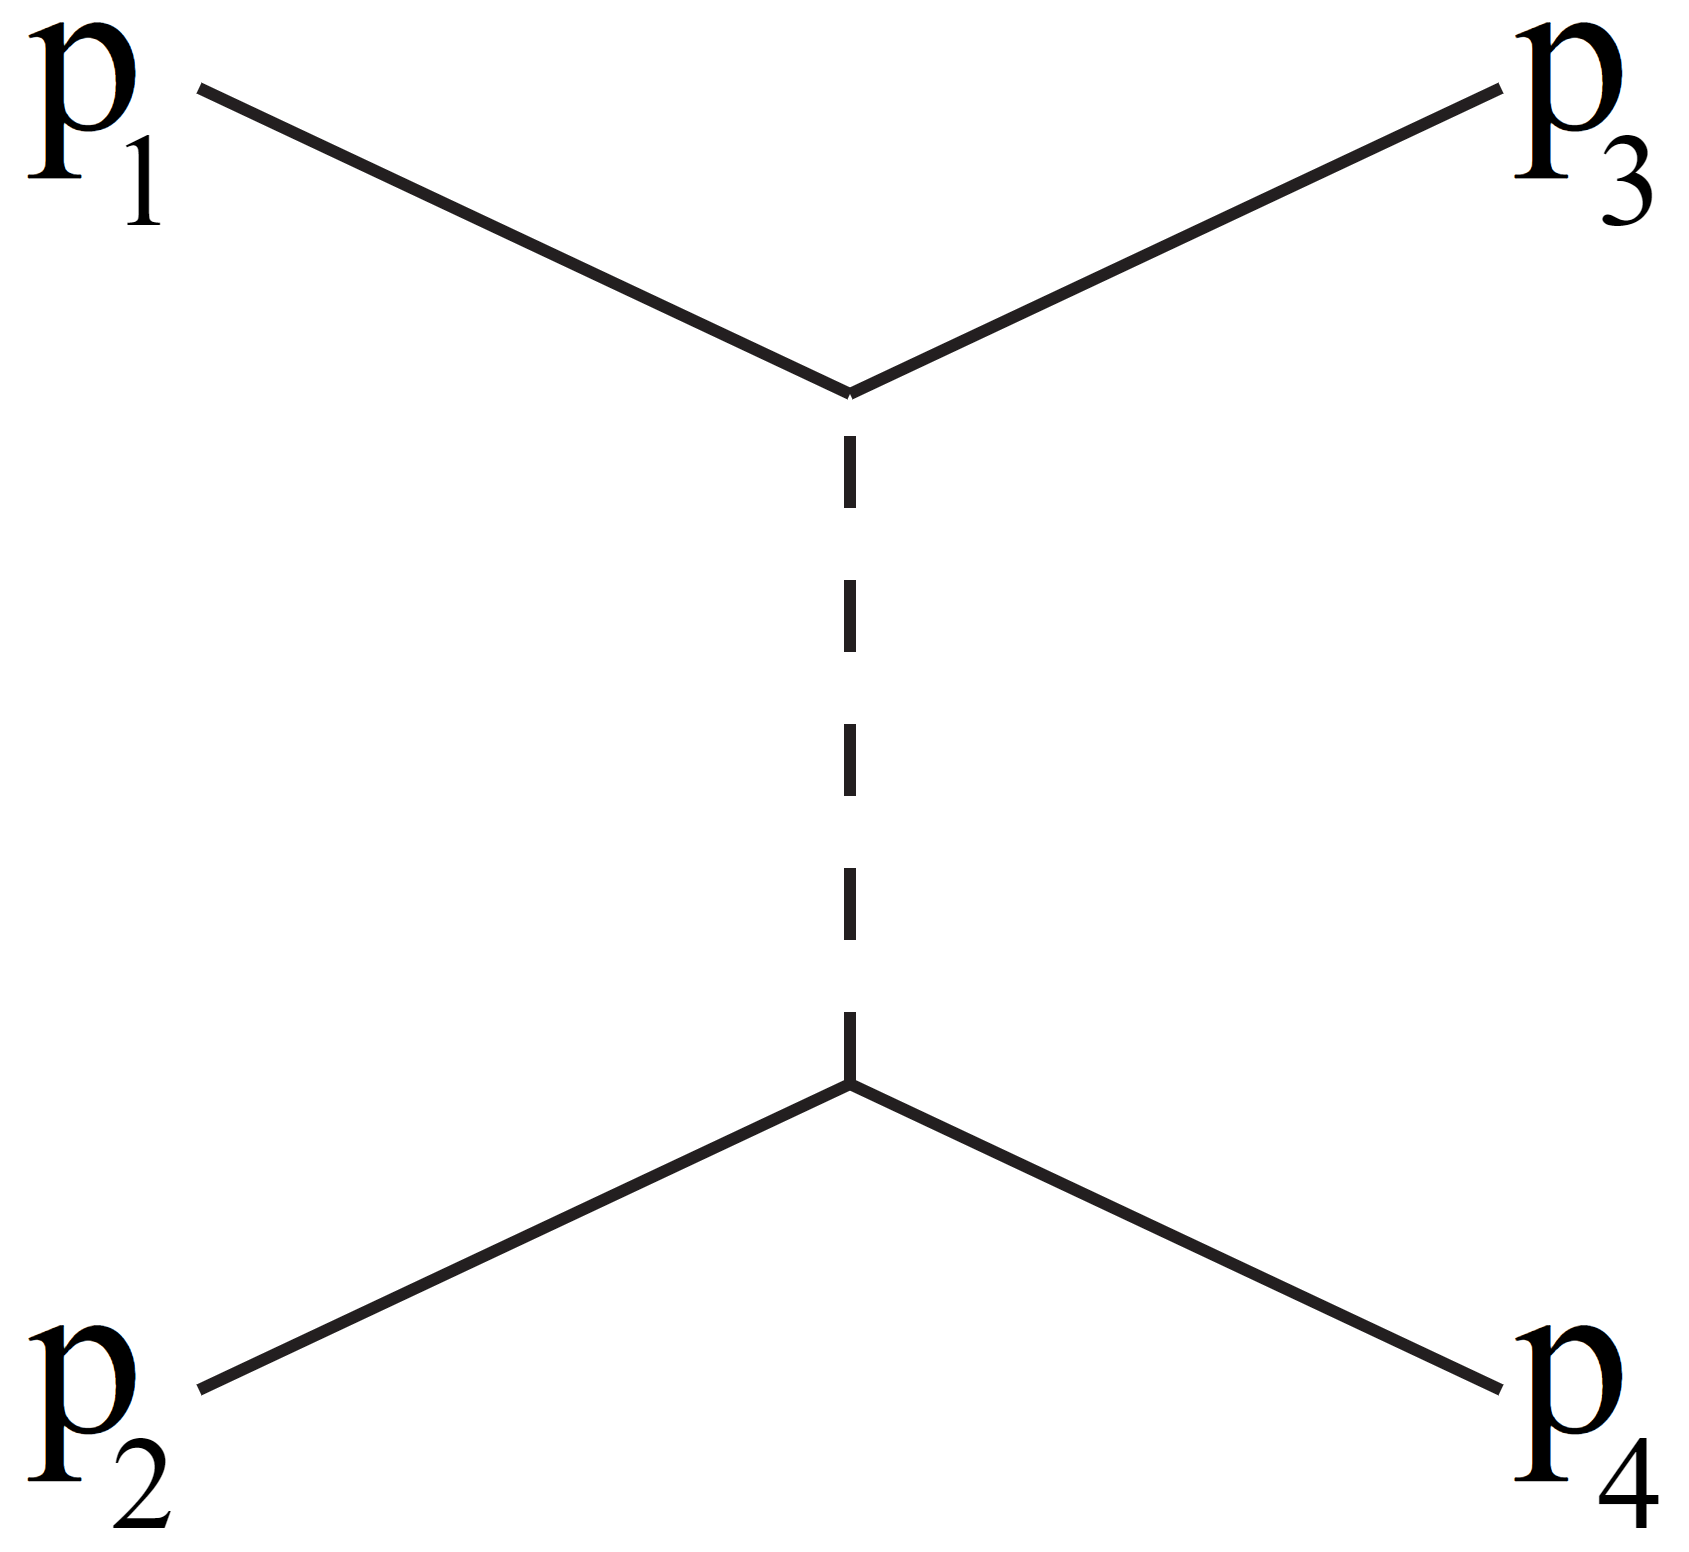
\includegraphics[width=0.35\columnwidth]{figures/Theory/TChannel.png}}
%	\caption{Feynman diagrams for (a) $s$-channel processes which could produce a new resonance and (b) $t$-channel background processes.
%	}
%	\label{fig:Feynman}
%\end{figure}



\chapter{The Large Hadron Collider and the ATLAS Detector}
\label{ch:LHCDetector}

\section{The Large Hadron Collider}
Section:LHC

\section{The ATLAS Detector}
Section:ATLAS
\subsection{Coordinate System}
Coords
\subsection{Magnet Setup}
Magnets yay, toroid yay

\subsection{SubDetectors}
\subsubsection{Inner Detector}
Inner
\subsubsection{Middle Layers, EMCal, HCal}
Yup
\subsubsection{Muon Calorimeter}
Muons have to get picked up I guess
\subsection{Trigger and Data Acquisition}
All of these subsystems lead into actual data farm
\subsubsection{L1Calo}
\subsubsection{HLT}
\subsubsection{Data Farm Information}
%\subsubsubsection{Trigger Rates}
%\subsubsubsection{Amount of Data}
\subsubsection{Luminosity Measurements}

%%%%%%%%%%%%%%%%%%%%%%%%%%%%%%%%%%%%%%%%%%%%%%%
%%%%%%%%%%%%                                                                                                   %%%%%%%% 
%%%%%%%%%%%%                           BEN                                                                  %%%%%%%% 
%%%%%%%%%%%%                                                                                                   %%%%%%%% 
%%%%%%%%%%%%%%%%%%%%%%%%%%%%%%%%%%%%%%%%%%%%%%%
%The particle physics program at CERN uses some of the most complex machines ever built, and have required the efforts of thousands of people to design, commission, and maintain.  This section outlines the systems which are used to provide the collisions and measure their products.
%
%\section{The Large Hadron Collider}
%
%The Large Hadron Collider (LHC) is the worlds largest and most powerful particle accelerator, at over 27\,km in circumference and capable of accelerating protons a center of mass energy of 13\,TeV.  It is located 100 meters underground along the French-Swiss border at CERN, just outside Geneva, Switzerland.  The beams are brought to collisions at different points along the ring to four major experiments: ATLAS~\cite{ATLAS}, CMS~\cite{CMS}, ALICE~\cite{ALICE}, and LHCb.\cite{LHCb}
%
%Protons in the LHC start as hydrogen gas which is ionized, the protons of which are accelerated to 50\,MeV by the LINAC2 linear accelerator.  From here, particles are accelerated in a series of circular accelerators of increasing size, starting with the Proton Synchrotron Booster which raises their energy to 1.4\,GeV.  This is followed by the Proton Synchrotron (PS) (25\,GeV) and Super Proton Synchrotron(SPS) (450\,GeV), after which proton bunches are finally injected into the LHC where they are ramped up to their final collision energy.  For Run 1, the LHC operated $\sqrt{s}$ = 7 and 8\,TeV, while in the ongoing Run 2 at $\sqrt{s}$ = 13\,TeV.  The CERN accelerator complex is shown in Figure~\ref{fig:AcceleratorMap}.
%
%\begin{figure}[h!]
%	\centering
%	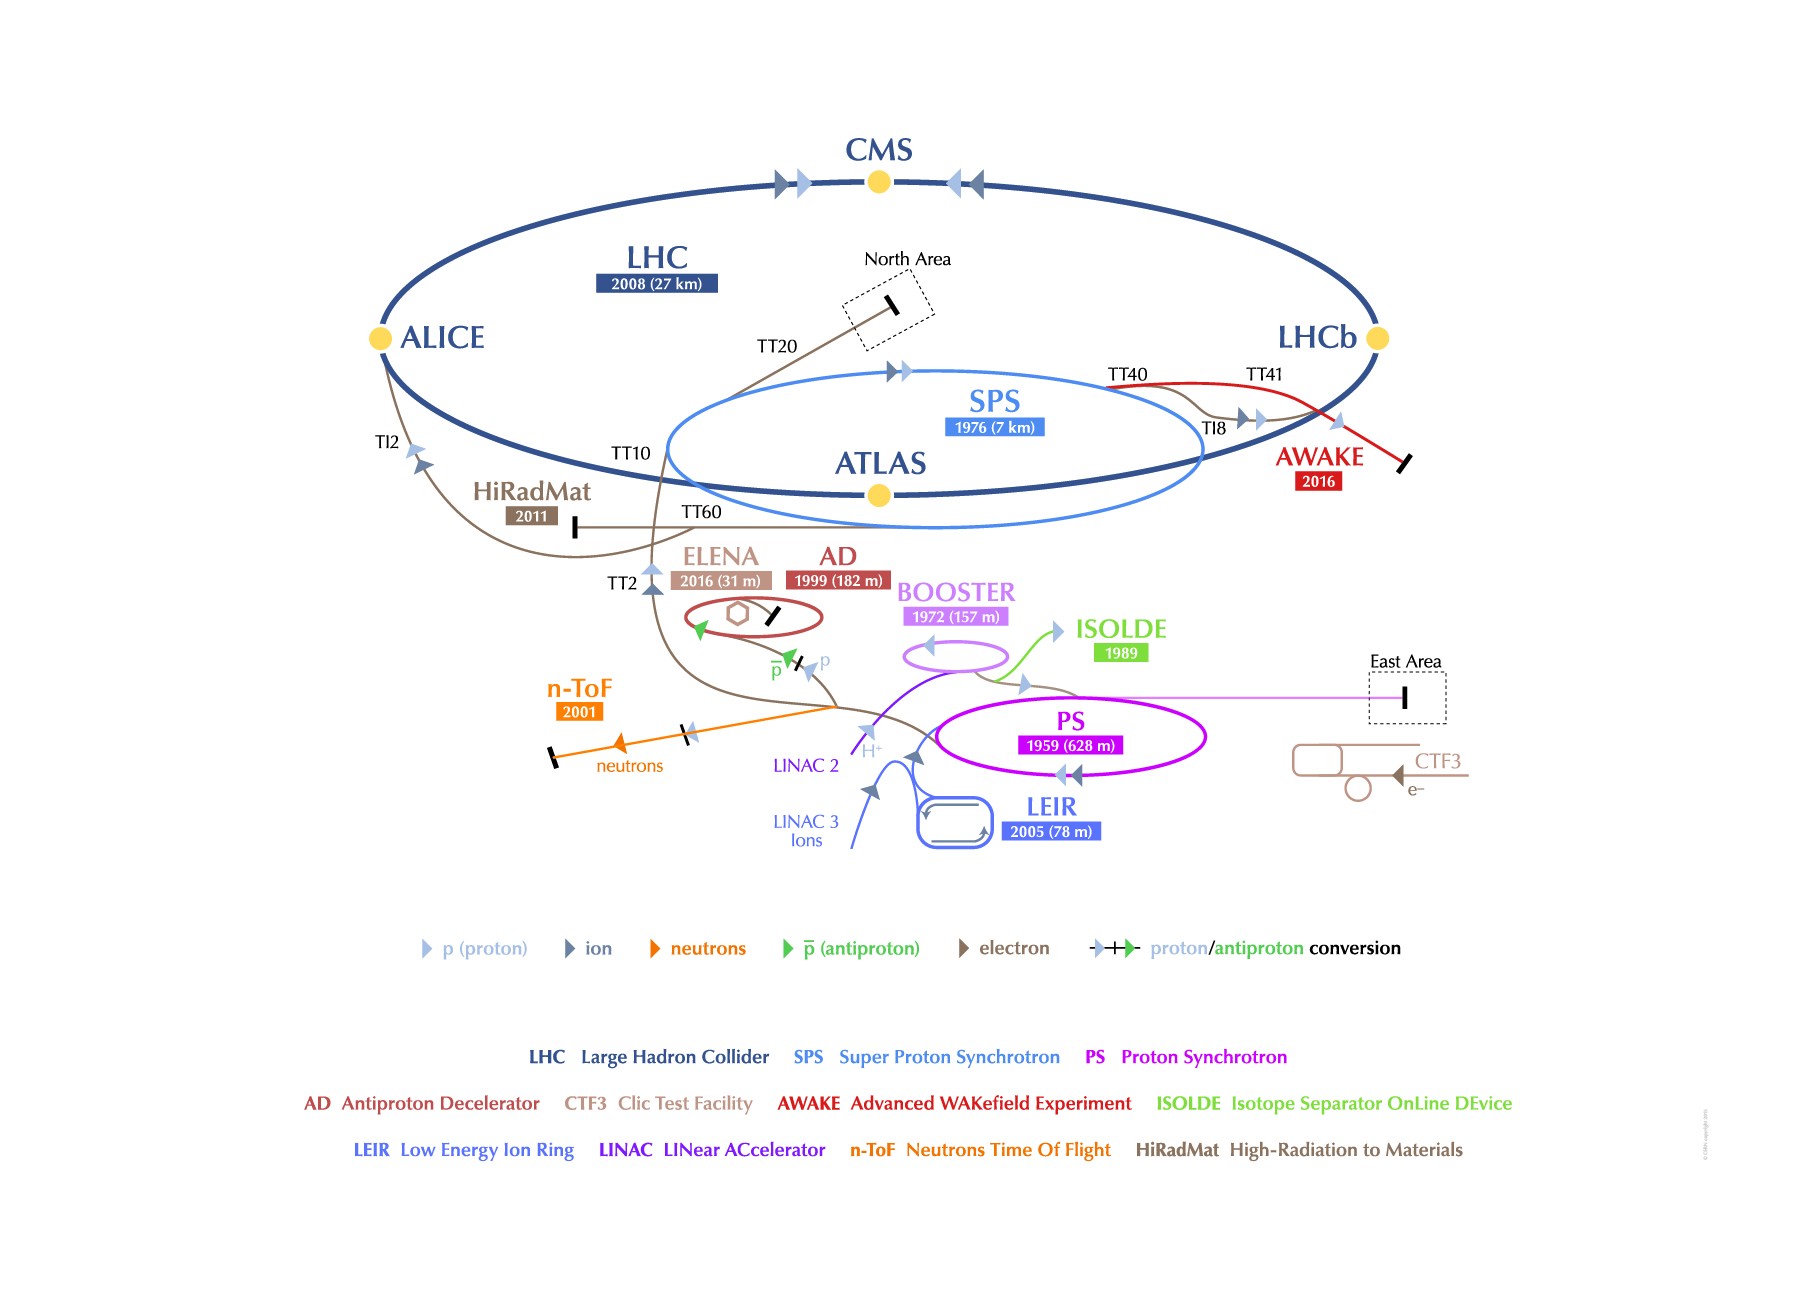
\includegraphics[width=\columnwidth]{figures/Detector/CERNAcceleratorComplex.jpg}
%	\caption{Schematic of the CERN accelerator complex.\cite{DeMelis:2119882}
%	}
%	\label{fig:AcceleratorMap}
%\end{figure}
%
%\subsection{Bunches and bunch trains}
%
%The LHC operates at a radio frequency (RF) of 400\,MHz which can be filled with bunches every 10 RF buckets for a separation of 25\,ns between bunches.\cite{Boussard:410377}  During Run 1 and the early part of Run 2 the LHC operated with 50\,ns spacing to reduce the effect of the electron cloud, but moved to the design spacing of 25 ns for the remainder of Run 2 data taking at the insistence of the detector collaborations.  This spacing, coupled with the $\sim27$\,km circumference of the LHC, means there are 3564 bunches which could be filled in the ring at any time.  In practice the LHC never fills all of these bunches at once, but instead the bunches are organized into $trains$.
%
%Bunch trains are groups of sequentially filled bunches in the machine and are driven by the design of the PS and SPS rings.  For a typical 2016 run, a single injection from the PS to the SPS was 72 sequential bunches, while the SPS transferred 288 bunches (4$\times$72) at a time over to the LHC.\cite{Bartmann:IPAC2017-TUPVA007}  The gaps between each of these bunches are driven by the kicker magnet rise times for each of these systems.  The minimum kicker times for the PS and SPS are 200\,ns and 800\,ns respectively, so each 72 bunch train is separated by 8 empty bunches, and each grouping of 288 is separated by 32 empty bunches.  The filling scheme also includes an abort gap, a space of approximately 100 empty bunches which is used in the case that the beam needs to be redirected to the beam dump.  In total, the number of filled bunches in the machine caps out around 2800 at a time.
%
%While the overall luminosity can be directly increased by upping the number of bunches in the machine at one time, the LHC has also tested other filling schemes which reduce the number of filled bunches but increase the charge in each bunch, or decrease the beam emittance, leading to a higher instantaneous luminosity and overall integrated luminosity.
%
%\section{The ATLAS Detector}
%
%The ATLAS detector is a multipurpose physics detector, located at Point 1 on the LHC ring near the main CERN site.  ATLAS weighs in at around 7000 tons, and is 44\,m long and 25\,m in diameter.  The detector is composed of multiple layers which measure their own unique portions of the collision products, which are described in the following section.  Figure~\ref{fig:AtlasDetector} shows how these systems are laid out.
%
%\begin{figure}[h!]
%	\centering
%	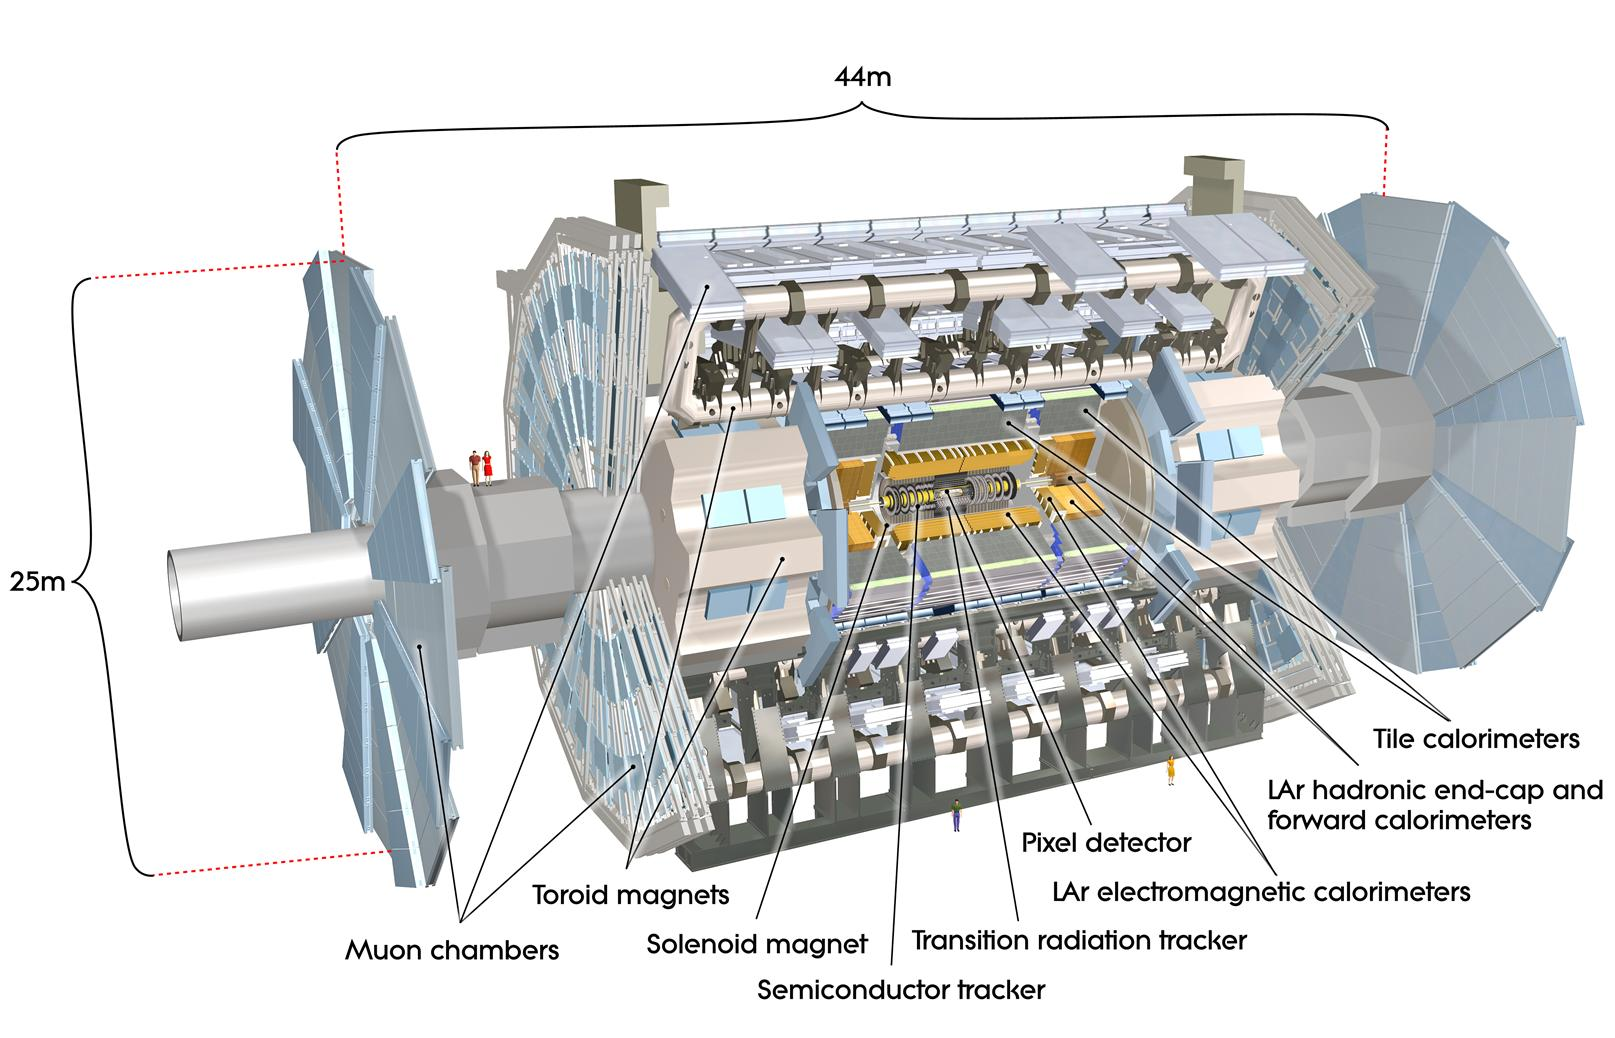
\includegraphics[width=\columnwidth]{figures/Detector/AtlasDetector.png}
%	\caption{A cutaway view of the ATLAS detector showing the various components.\cite{ATLAS}
%	}
%	\label{fig:AtlasDetector}
%\end{figure}
%\subsection{Coordinate System}
%
%The ATLAS experiment uses a right-handed coordinate system, with the origin at the nominal interaction point (IP) in the center of the detector.  The x-axis points from the IP towards the center of the LHC ring, and the y-axis points upward towards the surface.  ATLAS uses a cylindrical coordinate system which defines a radial distance $r = \sqrt{x^2+y^2}$ and azimuthal angle $\phi$ around the z-axis.  Instead of using the polar angle from the beamline $\theta$, pseudorapidity is typically used, defined as $\eta = -\ln{(\tan{\frac{\theta}{2}})}$.
%
%Massive objects, such as jets, are measured to have a rapidity defined as $ y = \frac{1}{2}\ln{\frac{E+p_z}{E-p_z}}$.  In the limit where $\pt \gg m$, as is often the case in this search, $y \approx \eta$, meaning that the rapidity of a jet and its detector location given by pseudorapidity are approximately interchangeable.  Differences in rapidities are Lorentz-invariant under z-axis boosts, making them useful for measuring if two jets are back-to-back in their rest frame.
%
%\subsection{Magnet System}
%
%ATLAS is composed of four separate magnets: one central solenoid encompassing the ID, one barrel toroid, and two endcap toroids.  The central solenoid provides a 2.0\,T magnetic field and is responsible for bending charged particle tracks near the IP to measure their momentum.  The namesake toroids provide a peak field of 4.0\,T, bending muons in a different plane than the solenoid field does to improve their momentum measurement.
%
%\subsection{Inner Detector}
%
%The ATLAS Inner Detector (ID) is comprised of three different subsystems: the silicon pixel layers (including the Insertable B-Layer (IBL) new in Run 2), the semiconductor tracker (SCT), and transition radiation tracker (TRT).  In total, the system covers the angular range $|\eta|<2.5$.  Information from all three subsystems is used to reconstruct tracks down to \pt = 0.4\,GeV.\cite{IDPerf}
%
%\subsubsection{Pixel and Semiconductor Trackers}
%
%The pixel detector system is composed of four concentric layers of silicon pixels, providing multiple high-resolution hits for charged particles traveling through.  The closest layer to the beampipe, the IBL, was added during Long Shutdown 1 (LS1) before the start of Run-2 operations.  At only 3.3\,cm away from the beamline, this additional tracking layer greatly improved the efficacy of tracking algorithms by an additional hit for tracks passing through multiple layers, and allowing for better resolution of secondary decay vertices, such as those originating from b-quarks.  The IBL also contains newer technologies than the rest of the pixel system which allow it to withstand the harsh radiation close to the beampipe.  This will allow the IBL to continue performing well as the innermost layer of the old pixel system degrades due to radiation, allowing for the maintenance of the current tracking performance.
%The SCT uses silicon microstrips and sits just outside the pixel system.  It is comprised of four barrel layers and 18 endcap disks (9 on each side of the detector), and range from 30 to 51\,cm from the beamline, adding additional position information for track finding.
%
%\subsubsection{Transition Radiation Tracker}
%
%The TRT operates on a very different principle than the other two tracking systems, taking advantage of the energy emitted when high energy particles transition between media with differing indices of refraction.  It is comprised of nearly 300,000 polyimide straws with an external aluminum layer and central gold-plated, tungsten wire at the center of each 4mm diameter tube.  The straws are filled with a gas mixture of Ar, CO$_2$, and O$_2$, and are ionized either by charged particles passing through or by emitted transition radiation.  Each straw hit provides additional 2-D hit information for track finding, as well as acting as a discriminant in electron identification.
%
%The TRT is scheduled to be removed as part of the ATLAS Phase-II upgrade starting in 2025, as the pileup conditions in Run 4 are expected to create TRT occupancies near 100\%, significantly degrading the performance of the system. The average TRT occupancy as a function of the number of interactions per crossing is shown in Figure~\ref{fig:TRTOccupancy}.  
%
%\begin{figure}[h!]
%	\centering
%	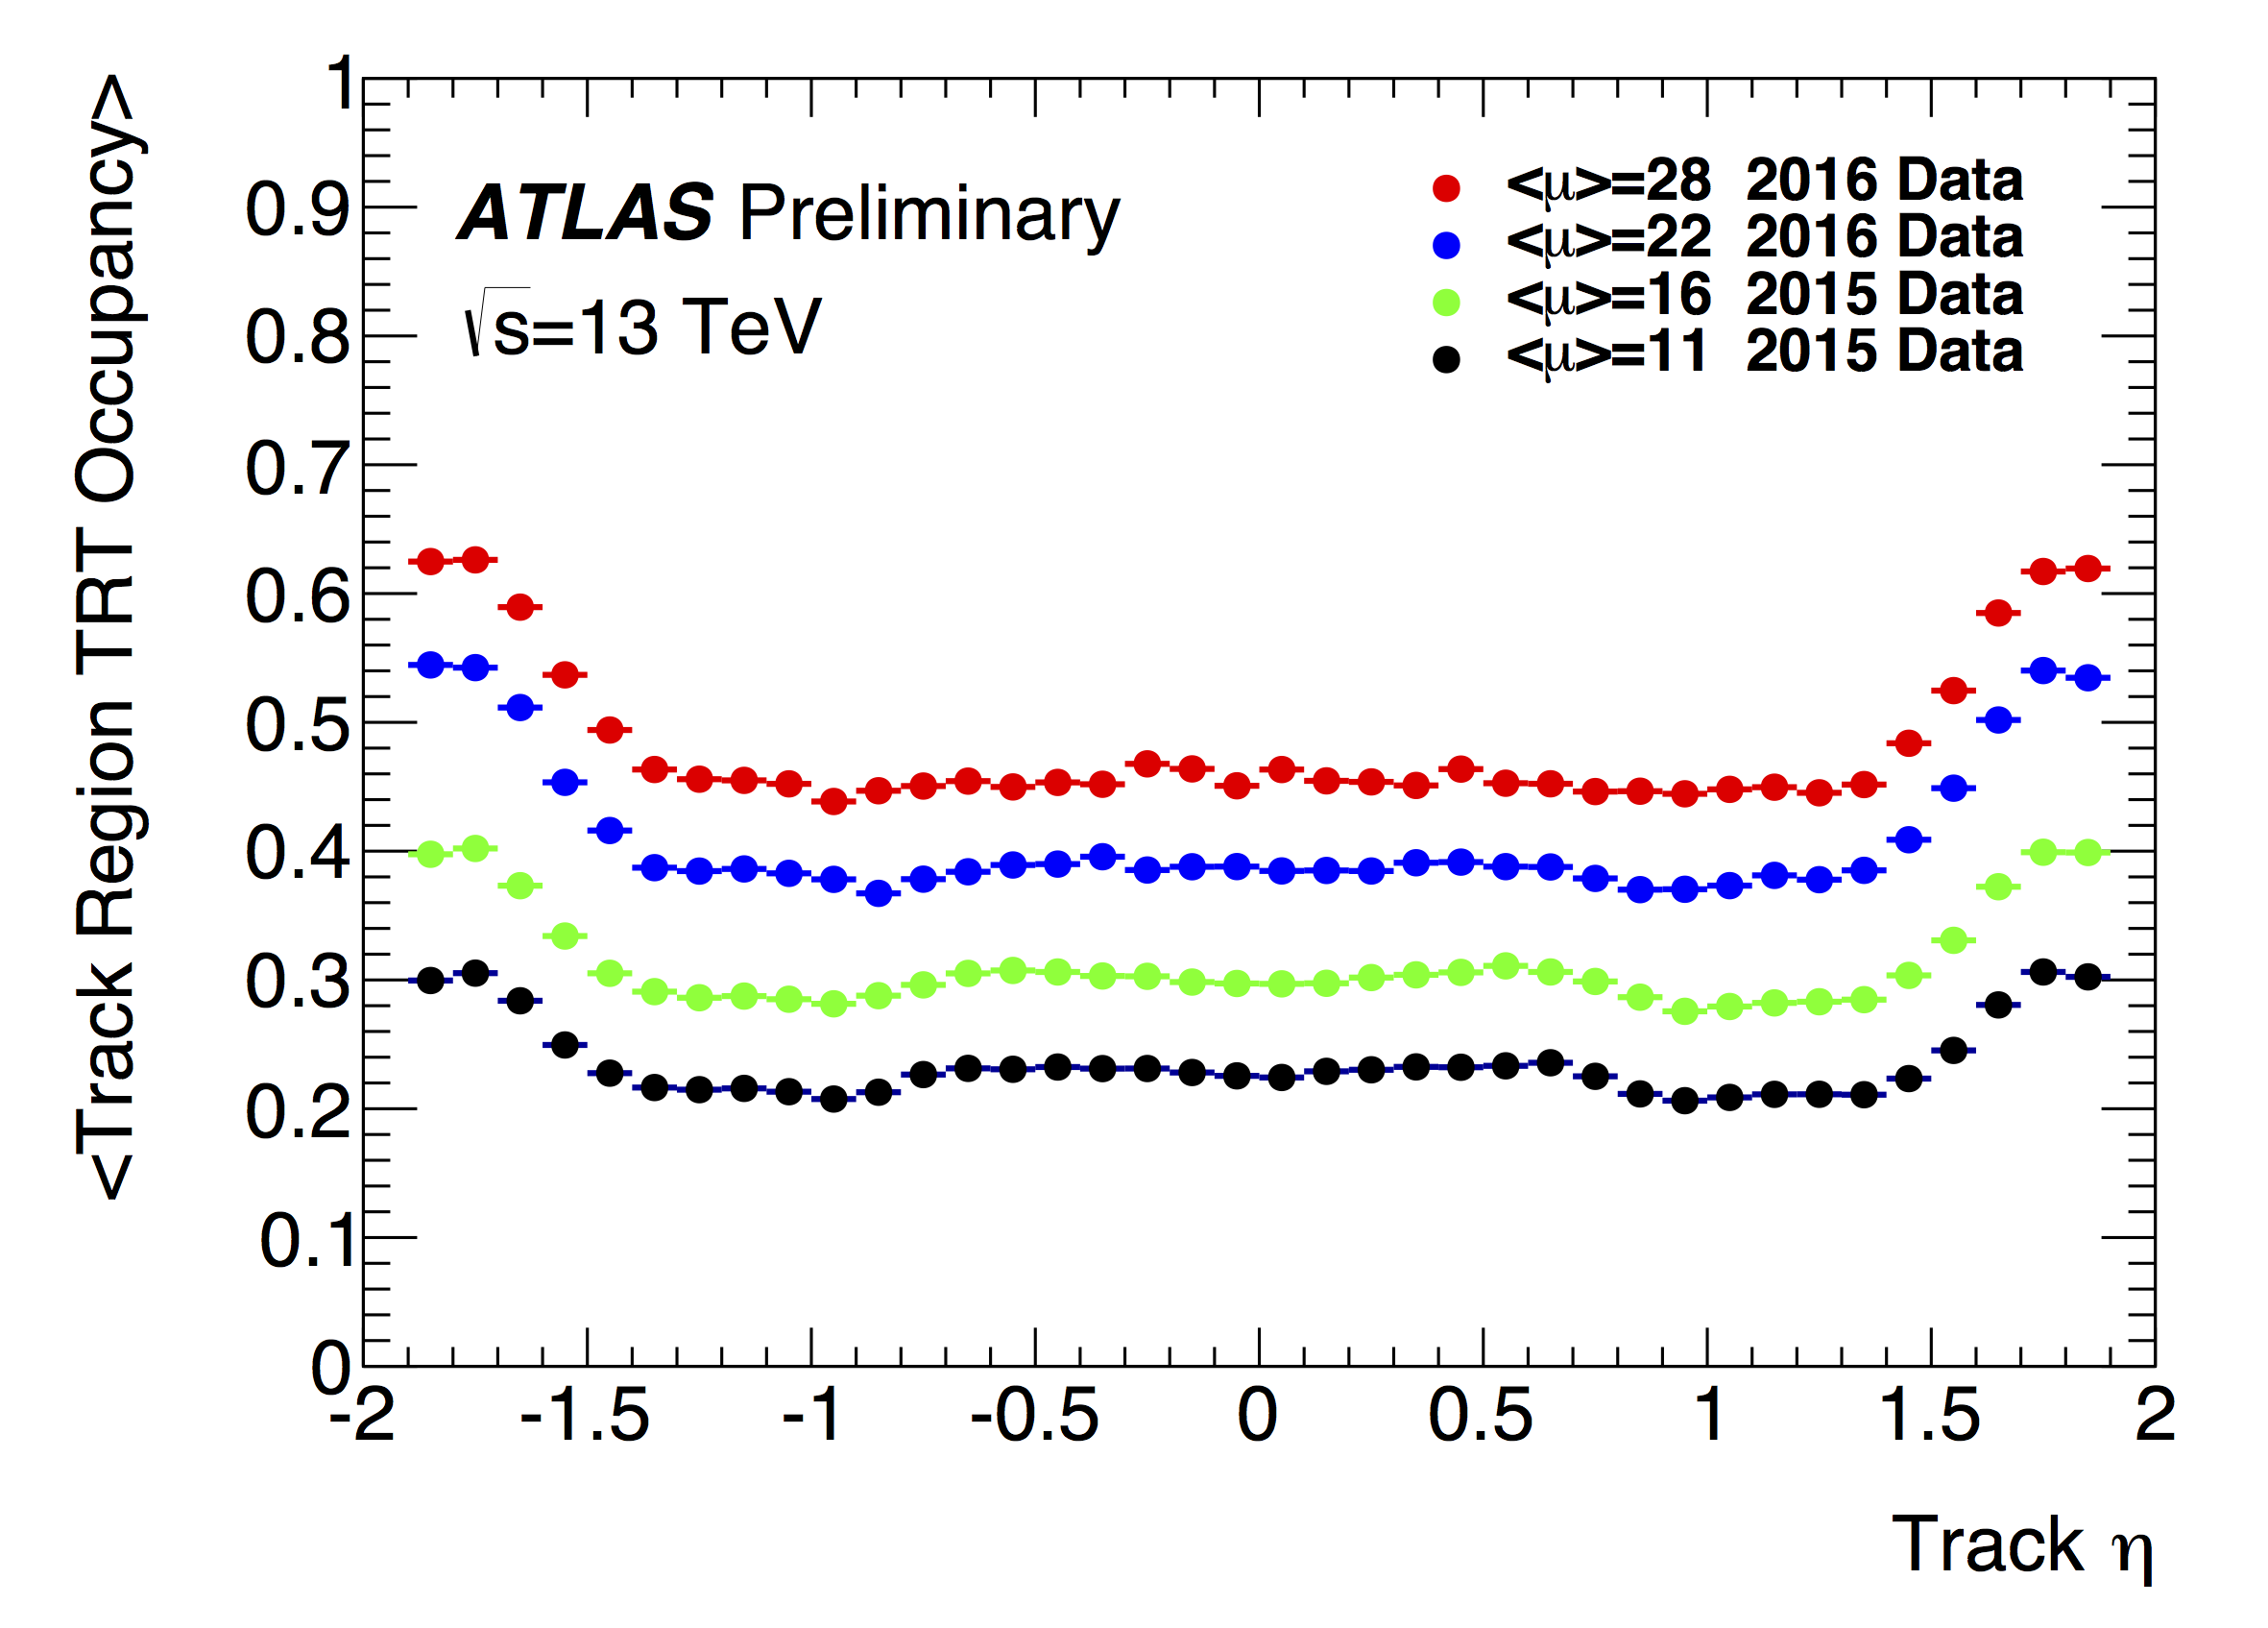
\includegraphics[width=0.6\columnwidth]{figures/Detector/TRTOccupancy.png}
%	\caption{Average track region TRT occupancy as a function of track $\eta$ using data taken during the 2015 and 2016 ATLAS runs for four different values of the average interactions per bunch crossing.
%	}
%	\label{fig:TRTOccupancy}
%\end{figure}
%
%\subsection{Calorimeters}
%
%ATLAS uses two different types of calorimeters to measure the energies of leptons, hadrons, and photons.  First is the liquid argon (LAr) electromagnetic calorimeter, which captures most of the energy from EM showers.  Second is the steel-scintillator Tile calorimeter which captures the energy from hadronic showers.  Optimal performance of the calorimeter systems under challenging conditions is vital to nearly every physics signature ATLAS searches for.  The system has nearly hermetic coverage in $\phi$ but is made up of several overlapping systems and varying thicknesses of material in $\eta$, and so special care must be taken to accurately calibrate the detector response in each region of the detector.
%
%The journey from calorimeter hits to the eventual trigger is discussed in detail in Chapter~\ref{ch:Calorimetry}.
%
%\subsubsection{Electromagnetic Calorimeter}
%
%The EM calorimeter uses liquid argon as an active medium, a choice motivated by the need for radiation-hardness, especially over the 30+ year run time of the LHC.  The calorimeter is composed of accordion shaped absorbers of lead with steel backing, with liquid argon flowing between and copper electrodes which measure the energy deposited.
%
%The LAr calorimeter is a sampling calorimeter, meaning that only a small fraction of the total energy from a particle traversing it is actually measured.  The power of an absorbing material is given by its radiation length ($X_0$), the distance an electron must travel in that material for its energy to be reduced by a factor of $\frac{1}{e}$.  Liquid argon is not dense enough as a medium to fit in a reasonable size calorimeter, and so lead (with a radiation length 20$\times$ shorter) is used to slow down the particles.  The EM calorimeter contains enough material to fully contain all but the largest electromagnetic showers, typically 25-30 interaction lengths depending on the region of the detector.  The actual pulse observed in the calorimeter is created when charged particles, showering from interactions in the absorber layers, cause the LAr to ionize and then release electrons which are accelerated by an electric field to the electrodes to become the calorimeter pulse.  The amount of energy actually measured by the LAr is much less than the total shower energy, and so it must be scaled back up by comparing the behavior of particles using test beam data where the incoming particle energy is well known.
%
%The EM Barrel covers the central region out to $|\eta|<1.475$, and two endcaps cover the range $1.375<|\eta|<3.2$.  The calorimeter is divided up into four layers of varying granularity, the first of which is the presampler.  This layer is closest to the inner tracker and has no absorber material in it, but instead is used to measure the amount of energy which has dissipated due to interactions with the material in the inner detector before it reaches the calorimeters.  The other three layers vary in thickness and granularity, and the values from each of these layers help determine the shape evolution of the shower as it progresses through the calorimeter, an important tool for electron/photon identification.  These pulses are read out and given to the level-1 trigger at coarse level, and if an event passes the trigger they are passed with full granularity to the high-level trigger.
%
%\subsubsection{Hadronic Calorimeter}
%
%Situated immediately outside the EM calorimeter, the hadronic calorimeter systems capture the remaining energy from hadrons which have already deposited a fraction of their energy in the EM layers.  The depth of material is characterized by the number of nuclear interaction lengths, the distance a hadron travels before undergoing an inelastic collision.  The depth varies as a function of $\eta$, but the hadronic calorimeters typically comprise 8-12 interaction lengths, enough to stop all but the most powerful showers.  In the barrel region, it is comprised of steel absorbing layers and scintillating polystyrene tiles, and the deposited energy is measured by molecular excitations in the scintillator emitting UV light which is then read out by photomultiplier tubes (PMTs).  The barrel systems covers the region $|\eta|<1.7$, but a different, more radiation-hard technique is required for the more forward regions.
%
%The Hadronic Endcap (HEC) covers the range $1.5<|\eta|<3.2$, and operates in largely the same manner as the EM systems.  Instead of the lead-steel combination of the EM layer, the HEC uses much thicker copper layers as the absorbers, with LAr still acting as the active medium.  The forward calorimeter (FCAL) covers the range $3.1<|\eta|<4.9$ and uses a combination of copper and tungsten plates as the absorbers.  Overall the hadronic calorimeters are much coarser than their EM counterparts, with a granularity of 0.1$\times$0.1 ($\Delta\eta\times\Delta\phi$) in the region $|\eta|<2.5$, and $0.2\times0.2$ in the forward regions.  
%
%\subsection{Muon Spectrometers}
%
%Muons interact very little with the calorimeters in ATLAS, leaving behind only tracks in the inner detector before they reach the outermost systems in ATLAS, the muon spectrometers.  In the muon systems, ATLAS's namesake toroids bend the tracks of passing muons to determine their momenta.  The muon system uses different technologies in the barrel and endcap regions, as well as different systems for triggering and momentum measurement.
%
%In the central region, monitored drift tubes (MDTs) are used to measure the tracks, and thus the momenta, of muons, while resistive plate chambers (RPCs) are used for triggering.  This split is required because of the long drift time of the MDTs of ~700\,ns, which is outside of the window the level-1 trigger system can use.  To deal with the higher backgrounds in the forward regions, cathode strip chambers (CSCs) are used for momenta measurements and thin-gap chambers (TGCs) are used for triggering.
%
%The muon system operates under the assumption that all other particles will be fully absorbed in the calorimeter layers, and thus any detected particles in the region must be muons.  However, in the case of very high-\pt jets some of the energy can "punch through" the calorimeters and register hits in the muon system.  This effect must be compensated for and is discussed later in the context of jet calibration.
%
%\subsection{Forward Detectors}
%
%Further down the beampipe from the IP are the various forward detectors for ATLAS which are primarily used for luminosity and cross-section measurements.  LUCID (LUminosity measurement using Cerenkov Integrating Detector) sits 17\,m down from the IP and consists of quartz fiber bundles connected to PMTs which detect Cherenkov radiation as charged particles pass through the quartz.  The multiplicity is proportional to the amount of interactions taking place at the IP, and is therefore used to measure the instantaneous luminosity.  ALFA (Absolute Luminosity For ATLAS) uses Roman Pots 240\,m from the IP to detect protons at angles very close to the beamline; ALFA is used in dedicated runs to measure the total proton-proton cross-section.  ZDC (Zero Degree Calorimeter) sits 140\,m from the IP and is used to measure the amount of neutral particles (neutrons and photons) left as beam remnants once the rest of the beam has been bent away by the steering magnets of the LHC; this information is used as a minimum-bias trigger for ATLAS, and as a centrality measurement for heavy-ion collision data.  Finally, AFP (ATLAS Forward Protons) is new for Run 2, primarily focusing on diffractive physics in special low-luminosity runs.
%
%\subsection{Trigger and Data Acquisition}
%During nominal operations, the LHC provides collisions at a rate of 40\,MHz, or an event every 25\,ns.  As each event is slightly under 2\,MB of data, this represents an extraordinary amount of information, and is far more than could be conceivably be written to disk, much less properly analyzed.  In order to reduce the data rate to a manageable level, and to ensure that only the events with the most interesting physics are saved, a two-tiered trigger system is used.
%\subsubsection{Level-1 Trigger}
%The level-1 (L1) trigger is hardware based, making decisions on whether or not to keep an event within 2.5\,$\mu$s.  For Run-2 operation, the L1 trigger reduces the event rate to a maximum of 100\,kHz.  The L1 trigger is made up of several subsystems which bring together decisions from different areas of the detector to make a final decision on whether or not to keep an event.
%
%The L1 calorimeter trigger (L1Calo) uses information from the EM and hadronic calorimeters in the form of rough 0.1$\times$0.1 ($\eta\times\phi$) trigger towers.  From this information, candidates for jets, electrons/photons, and taus are constructed and passed along as regions of interest (RoI) to the next stages in the trigger telling the type of object, its transverse momentum as measured at L1, and its location in the detector.  The amount of global missing transverse energy (MET) is also calculated and used as part of the trigger signature.  The L1Muon system uses a coincidence of hits in the RPCs and TGCs to identify muon candidates.  Since precision momentum information from the MDTs and CSCs takes too long for the L1 decision, the muon momentum is roughly estimated using the hit pattern, and then marked as being above one of a set number of \pt thresholds.
%
%Within each system, a list of pre-determined triggers are compared against the RoIs found in the event.  For example, the muon system has triggers for muons above 20\,GeV (L1\_MU20) as well as for two muons above 6\,GeV (L1\_2MU6).  The list of all triggers passed in each system is passed along to the Central Trigger Processor (CTP) where the final determination on whether or not to save an event is made.
%
%RoIs from both L1Calo and L1Muon are then sent to the L1 Topological trigger. (L1Topo)  Newly commissioned in 2016, L1Topo allows for more advanced combinations of trigger objects from the two systems, including operations such as invariant mass, angular separation between objects, and transverse mass.\cite{L1Topo}  This additional processing step greatly reduces the background rates for certain processes, allowing for much lower energy thresholds when using objects triggered from L1Topo.  Similar to L1Calo and L1Muon, the list of triggers passed by an event is passed along to the CTP.
%
%The CTP is the final stage of the L1 trigger.  It receives a list of all passed triggers from the other subsystems and compares it against an L1 trigger menu.  The trigger menu determines which triggers should be turned on or off during a given run, as well as the prescale, or rate reduction, rates for triggers.  Triggers with lower energy thresholds are often prescaled, meaning that only a fraction of events that pass a given trigger are kept.  For example, a physics menu item with a prescale of 20 will have only 1 out of 20 events that pass the trigger saved, while the other 19 times the event is not saved unless some other trigger is also passed and and marks the event for saving.  The L1 trigger menu evolves over the course of time as well as within a single physics run, changing the prescales of physics items to keep the rate of saved data as close to 100\,kHz as possible as the instantaneous luminosity decays.  If the CTP determines that an event passes at least one trigger after prescaling, then the event is saved.  At this point a level-1 accept signal is sent which triggers the readout of the full granularity detector data.  The result of which triggers were passed at the CTP, along with the RoIs, are then passed along to the high-level trigger.
%
%\subsubsection{High Level Trigger}
%
%Events passing the L1 trigger are fed to the High-Level Trigger (HLT), which uses the full detector readout and granularity to measure physics quantities at close to offline precision.  For Run 2, the HLT accepts events at nearly 100\,kHz and reduces this rate down to 1\,kHz for the general physics stream.  The HLT runs on a general computing cluster with thousands of cores and uses much more complex software algorithms for event analysis, such as b-tagging and anti-$k_t$ jet clustering.
%
%HLT trigger chains are seeded by an matching relevant L1 trigger.  For example, the single-jet trigger HLT\_j380 is seeded by the L1 trigger L1\_J100.  As events can pass multiple trigger thresholds and types, multiple HLT algorithms can be run on a single event.  Each HLT item corresponds to a chain of processing steps which are optimized to reject events as early as possible, using the full readout and precision processing steps only on the most likely candidates.  There are several different types of HLT chains which are used, including primary chains, the unprescaled standards used by most analyses, supporting chains, which are typically prescaled and are used mainly for determining backgrounds for other analyses in regions which can not support an unprescaled trigger, and monitoring chains, which readout only a small portion of the whole detector and are used to check the performance of specific subsystems.
%
%The debug stream includes events which are unable to be processed in the HLT, either due to them timing out after taking too long to process, or because of some issue which caused a crash.  All events which cause errors in the HLT are saved to the debug stream to ensure no interesting events are lost, and to troubleshoot which algorithms are problematic.  The debug stream typically only contains a handful of events per run, but on occasion HLT farm crashes have caused hundreds of thousands of events to be saved to it.  ATLAS also uses a data scouting stream which supports lower threshold physics searches by giving them drastically increased event rate in exchange for saving only a small portion of the event data.  This stream is used by the ATLAS Trigger Level Analysis (TLA) to look at dijet events in the invariant mass range below the reach of the standard dijet search.
%
%\subsection{Dead Time}
%
%The ATLAS detector is limited in how many events in can process in a given amount of time, leading to "dead time" for the detector when collisions are occurring and the detector is operating nominally, but events are unable to be saved.  The first type is referred to as simple dead time, which occurs after every L1Accept and takes about 100\,ns, or 4 bunch crossings.  During this time the detector is transferring the full readout to the front end buffers for processing in the HLT and can not save any other events.  The second type is complex dead time which comes about from the limited size of these readout buffers for individual subsystems and the rate at which data can be sent off-detector.  Complex dead time limits the number of accepted events in a given period of time; if too many events occur too quickly, the readout buffers fill up and events must be vetoed until there is space for another event in the buffer.  The complex dead times are controlled by four "buckets" which are adjustable between runs depending on the requirements of the different hardware subsystems, characterized by a max number of L1Accepts in a given number of BCs.  For example, 15/430 means that up to 15 events can be saved within a window of 430 BCs, and triggers are put on hold until the rate drops down below this level.
%For the dataset used in this analysis, ATLAS recorded data with 92\% efficiency. The total amount of dead time varies based on the luminosity, but typically covers $\sim3\%$ of collision time.  The remaining inefficiency comes from reducible sources such as detector errors which send a busy signal and hold triggering while the system fixes an issue or resets a component.
%
%\subsection{Data Processing}
%
%Events which are accepted by the HLT are written to disk and are passed to the ATLAS Tier-0 computing facility at CERN, where the detector readout is transformed from raw data into the physics objects that will eventually be used for analyses.  Immediately after a run is taken, the express stream (a small subset of the full physics data stream) is run through what is known as the calibration loop, a $\sim48$ hour process in which the geometry and conditions for the run are calculated to properly process the whole dataset.
%
%Once calibration is complete, the data enters bulk reconstruction where the full dataset is run through the standard ATLAS software to change the data from raw detector readout to containers which describe objects such as electrons and jets, or more granular objects such as track-candidates or calorimeter clusters.  This data format is known as xAOD, or Analysis Object Data.  This dataset is then duplicated around the world to the various computing facilities around the globe.  From here, the data is run through the Derivation Framework.
%
%To prevent analyses from needing to run over the entire ATLAS dataset, each group of analyses sharing a similar signature creates a specialized derivation which skims through the full dataset and only keeps events which are likely to be relevant to the analysis, and allows groups to remove unneeded data containers, or to create their own data containers which are not part of the standard set.  For example, the derivation which the dijet analysis uses keeps only events which pass one of the single- or multi-jet HLT chains, and gets rid of muon and electron data as those objects are not used in any way in the analysis.  The typical derivation is only$\sim1-2\%$ of the full AOD in size, making it much more manageable for analyses to run their search over.  These derived AODs (DxAODs) are then duplicated to multiple places in the CERN computing grid and become available for analysis use.  The main physics stream for ATLAS recorded 1.7 billion events in 2015 and 5.4 billion in 2016, comprising some 6.2 petabytes of raw data, making running over the full dataset exceedingly difficult!
\chapter{Simulation and Reconstruction}
\label{ch:Simulation}

% Notes: Should I put in how many events are simulated?

This chapter presents details on the simulation of various physics processes and the reconstruction of physics objects for both simulated events and data events.  

\section{Simulation of pp Collisions}
To draw conclusions from ATLAS experimental data it is necessary to make accurate theoretical predictions about the processes being searched for.  Having accurate background models can help identify when a data signal is behaving in a way that might suggest new physics.  Due to the stochastic nature of particle physics collisions and interactions, it is not practical to create exact predictions.  Instead the ATLAS experiment uses Monte Carlo (MC) simulations to model physical behaviors.  MC simulations are done by repeated random sampling of possible physical processes that can occur at any given time to a particle.  The possibilities change based on factors such as particle energy and particle environment.  A flow chart for the entire simulation chain is shown in Figure \ref{fig:SimMCFlow}. 

\begin{figure}[h!]
	\centering
	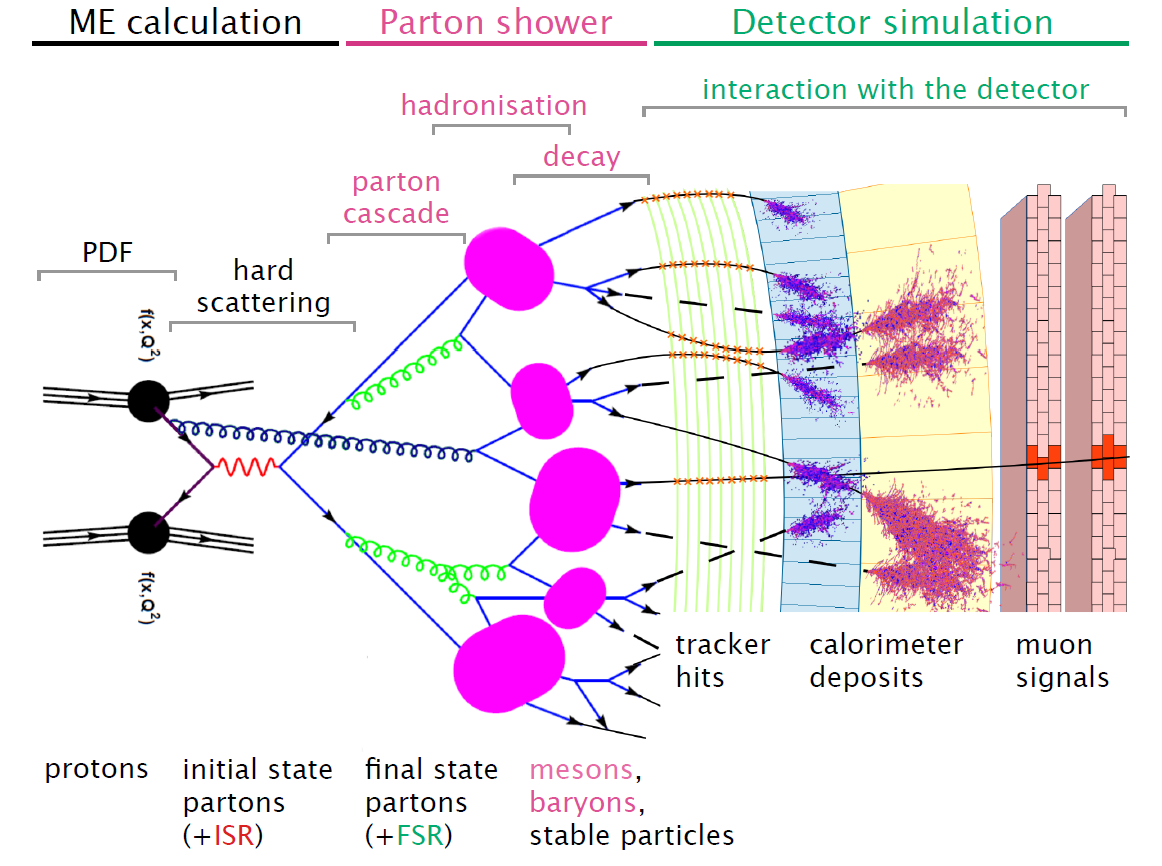
\includegraphics[width=\columnwidth]{../ThesisImages/Simulation/MCFlow.png}
	\caption[A pictoral view of the different steps for the creation of a MC event.]{A pictoral view of the different steps for the creation of a MC event. \cite{MaxThesis} 
	}
	\label{fig:SimMCFlow}
\end{figure}

\subsection{ Matrix Element Calculation and Parton Distribution Functions}

Particle interactions at LHC energies do not involve the entire proton.  The constituent partons that create the proton (the two up quarks, down quark, and the sea of gluons) are what interact in any given event.  The gluons create many virtual quark-antiquark pairs which can interact as well.  The valence quarks, the two up quarks and the down quark that make up the proton, are the major portion of interacting partons at low energies, mainly inelastic interactions.  At LHC energies deep inelastic scattering is possible and the sea quarks play a more dominant role.  Proton structure is described by a Parton Distribution Function (PDF) which gives the probability of finding any parton with a particular momentum fraction, is shown in Figure \ref{fig:PDF}.

\begin{figure}[h!]
	\centering
	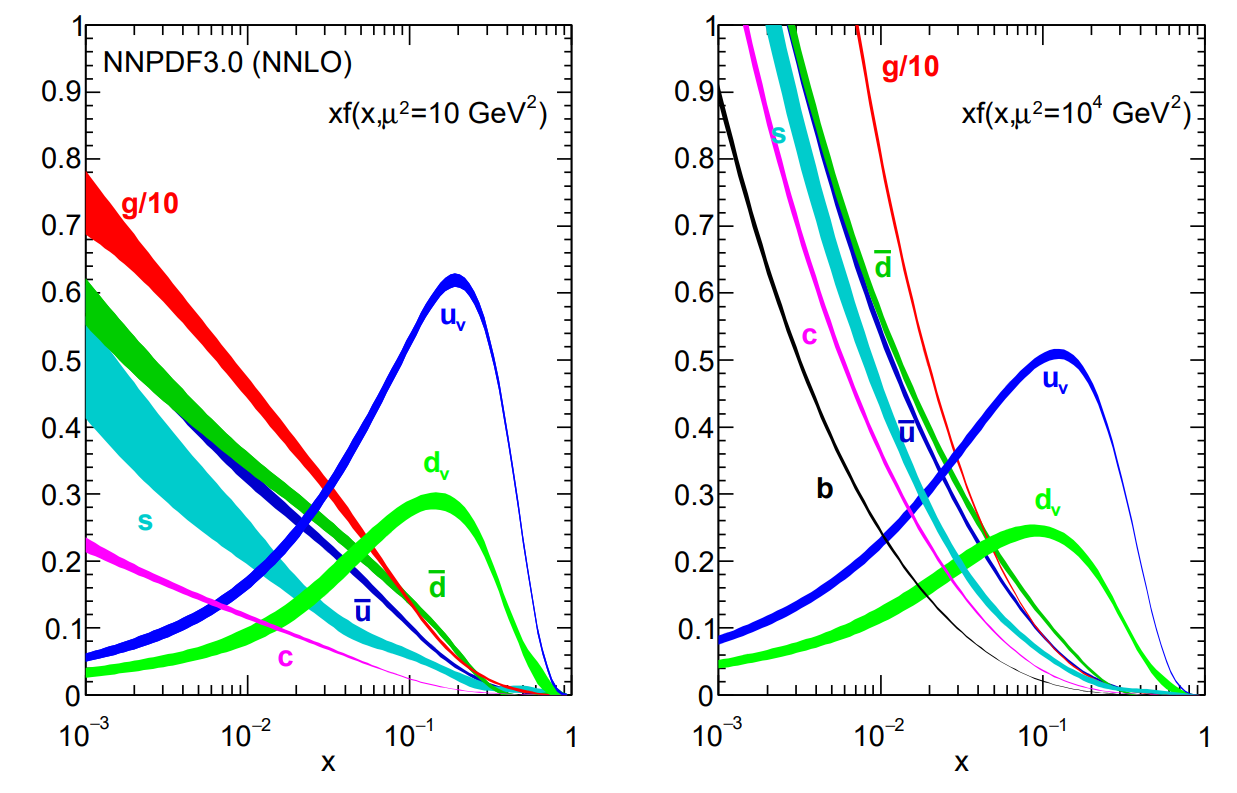
\includegraphics[width=\columnwidth]{../ThesisImages/Simulation/PDF.png}
	\caption[The bands are the momentum fraction, $x$, times the unpolarized parton distribution function obtained in NNLO NNPDF3.0 global analysis at scales $\mu^2= 10$ GeV and $\mu^2 = 100 \text{ GeV}^2$]{The bands are the momentum fraction, $x$, times the unpolarized parton distribution function obtained in NNLO NNPDF3.0 global analysis at scales $\mu^2= 10 \text{ GeV}^2$ and $\mu^2 = 100 \text{ GeV}^2$ \cite{PDG2018} 
	}
	\label{fig:PDF}
\end{figure}
The PDFs and hard scattering processes are included in the calculation of the Matrix Elements (ME) of any interaction.  Hard scattering processes can be descibed by Feynman diagrams, a representation of their amplitudes.  Combining the PDFs and hard scattering amplitudes gives the probability of a particular interaction occuring.  Calculation of the MEs is the first stage of simulation and is done to a specified order in perturbation theory: leading order (LO), next-to-leading order (NLO), etc.  Higher order calculations lead to more accurate predictions but grow in complexity exponentially making them harder to calculate both theoretically and computationally, often restricting how accurate a process can be simulated.  

\subsection{Parton Shower Calculation}
The next stage of simulating an event is the parton shower.  These parton shower calculations deal with the quantum chromodynamic processes.  In any interaction the particles that carry color can spontaneously emit gluons which can go on to create more gluons or quark-antiquark pairs.  Depending on when this happens in the hard scattering process it is called initial state radiation (ISR) or final state radiation (FSR).   The hard scattering partons as well as any additional radiated particles are used as inputs to parton shower calculations which determine how the quarks and gluons proceed through to the final state particles seen in the detector.  This includes calculation of hadronization processes and futher decay processes into the final state particles.

\subsection{Detector Simulation}
The final stage of creating an MC event is the detector simulation.  The information from the event generators are processed using \textsc{geant4} \cite{Geant4} and a detailed model of the ATLAS detector.  \textsc{geant4} simulates how various particles propagate through and interact with the material properties of the detector and where they leave energy which would then be measured by the ATLAS detector in an actual event.  The result of this MC event construction flow is a collection of simulated data that is similar in structure to actual data collected using the ATLAS experiment.  The energy deposits in both MC and real data are combined using the same software for physics objects are reconstruction.  For MC events this allows for comparison between the physics object reconstruction and the truth record, or the types of particles fed into the detector simulation.

\subsection{Monte Carlo Generators Used for LHC Physics}

A variety of different MC generators are used in the creation of simulated events.  Different generators specialize in simulating different physics processes to various levels of precision (eg., LO vs. NLO). The MC generators used in this search are summarized in this section.

\textsc{MadGraph} aMC@NLO \cite{MadGraph}: An amplitude and event generator at LO and NLO for hard processes.  Extendable to various models including effective field theory (EFT) models used in BSM searches.  This generator is used to create the signal events searched for in this dissertation: discussed in Section \ref{Sec:MG5Sig}. 

\textsc{powheg} \cite{Powheg1,Powheg2}: \textbf{Po}sitive \textbf{W}eight \textbf{H}ardest \textbf{E}mission \textbf{G}enerator is an NLO event generator that can be interfaced with other generators (i.e. \textsc{pythia}) for showering.

\textsc{pythia} \cite{Pythia8}: A generator used most often for QCD final state hard processes and showering.  It is commonly interfaced with other generators for showering within the ATLAS detector.

\textsc{sherpa} \cite{Sherpa11,Sherpa22}: A multi-parton LO generator with an emphasis on merging ME and Parton Showering.

A common event file format developed at the Les Houches Accords \cite{Alwall:2006yp} makes it possible for these generators to be interfaced in a straight forward way, typically with \textsc{pythia} for showering.  This allows a specialty generator to be created and used to generate hard processes and then simulate the rest of the event with common showering generators that might lack the ability to simulate the process in question.



%%%%%%% FCNC Generation
\section{Creation of Flavor Changing Neutral Current Signal Events}
\label{Sec:MG5Sig}
To create simulated signal events the typical Standard Model models must be extended to include higher order terms.  A Universal FeynRules Output (UFO, \cite{UFO})   model was created to include dimension 6 operators (\cite{Dim6TermsOld, Dim6Terms}).  These individual operators are turned on for the specific final state being produced.  The original operators can be reduced to a minimal set of coupling to anomalous finals states (i.e. FCNC final states)\cite{TopCouplingsAguilarSaavedra}, used for event production.  This effective field theory method of signal production is beneficial as it allows for production of signal events that are not dependent on any particular BSM model.  This method of including dimension-6 effective operators can be used to produce any of the top FCNC channels, for example in the $t\rightarrow qZ$ process \cite{FCNCtqZ} and $t\rightarrow qH$ \cite{UFOModel}.

\subsection{FCNC Events Produced With MadGraph5 aMC@NLO}

Signal events have been produced using MadGraph5 aMC@NLO following the Work of Degrande et al.\cite{Degrande:2014tta}.  Before official ATLAS datasets can be produced and the entirety of the event reconstructed through the ATLAS detector, validation of the model must be performed.  10,000 events were produced locally at truth level for each decay channel to compare the kinematics of produced events in $t\bar{t}\rightarrow bWq\gamma$ to the kinematics of official production $t\bar{t}$ events. 

\begin{figure}[h!]
	\centering
	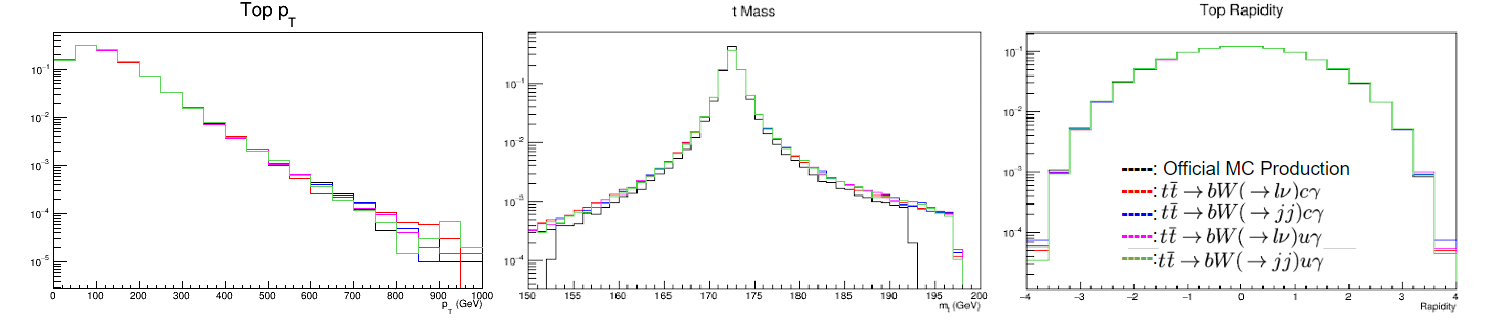
\includegraphics[width=\columnwidth]{../ThesisImages/FCNCValidation/singleTops.png}
	\caption{ Normalized kinematics ($p_T$, $m_t$, and $y_t$) of individual top quarks produced by the model for each FCNC final state search and an official $t\bar{t}$ sample.
	}
%	\label{fig:SimMCFlow}
\end{figure}


The minimal couplings mean there is one scalar coupling introduced for each decay mode, $t\rightarrow c\gamma$ and $t\rightarrow u\gamma$.  All possible final states are shown in the figures in this section: the leptonic and hadronic decays of the W boson from the top quark that decays through the typical standard model decay mode $t\rightarrow bW$. 

\begin{figure}[h!]
	\centering
	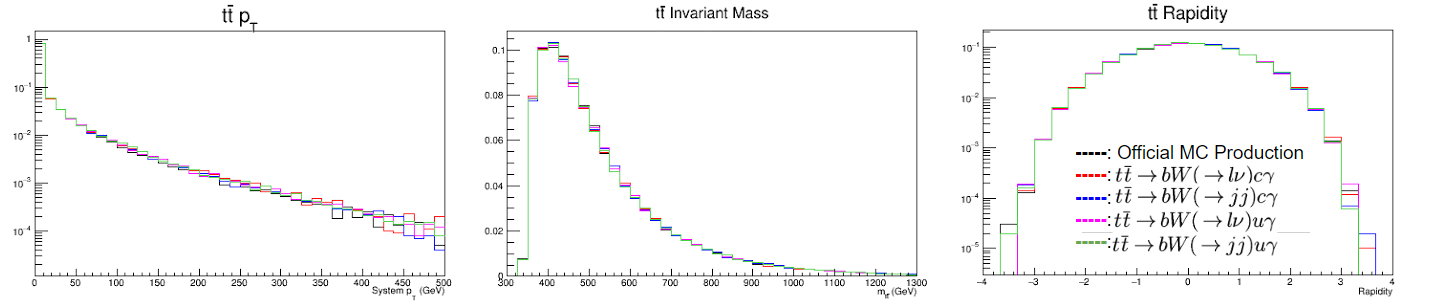
\includegraphics[width=\columnwidth]{../ThesisImages/FCNCValidation/ttBarSys.png}
	\caption{Normalized kinematics ($p_T$, $m_{t\bar{t}}$, and $y_{t\bar{t}}$) of the $t\bar{t}$ system produced by the model for each FCNC final state search and an official $t\bar{t}$ sample.
	}
%	\label{fig:SimMCFlow}
\end{figure}

\begin{figure}[h!]
	\centering
	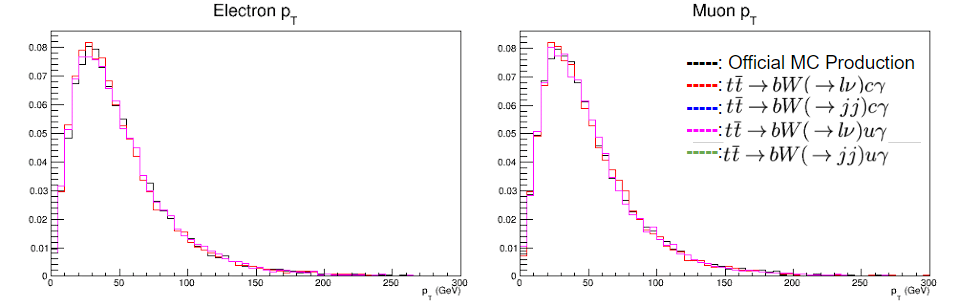
\includegraphics[width=\columnwidth]{../ThesisImages/FCNCValidation/lepton.png}
	\caption{Normalized $p_T$ of the electron and muons produced by the model for each FCNC final state search and an official $t\bar{t}$ sample.
	}
	\label{fig:LepVal}
\end{figure} 

The lepton validation plots in Figure \ref{fig:LepVal} only show events where the W is forced to decay leptonically as well as the official sample which does not have a preference for the final state decay, i.e., the W bosons are allowed to decay leptonically or hadronically.  
\begin{figure}[h!]
	\centering
	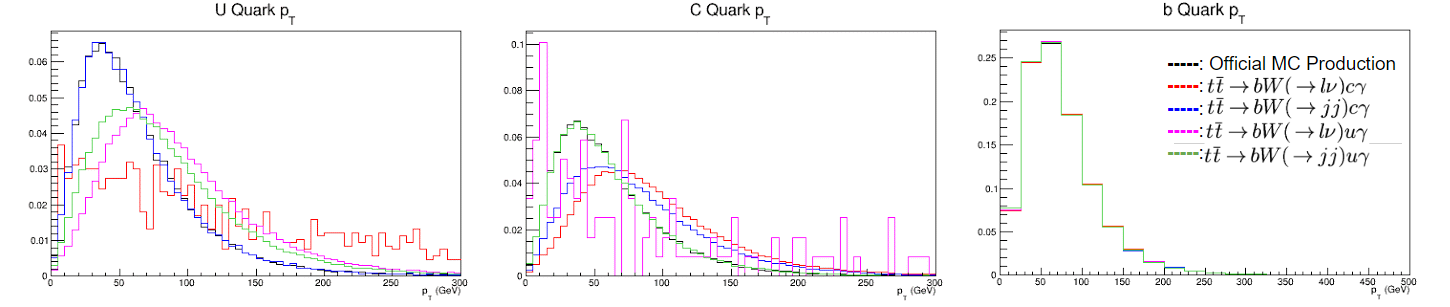
\includegraphics[width=\columnwidth]{../ThesisImages/FCNCValidation/quarks.png}
	\caption{Normalized $p_T$ of the up, charm, and bottom quarks produced by the model for each FCNC final state search and an official $t\bar{t}$ sample.
	}
	\label{fig:QuarkVal}
\end{figure}
No unexpected deviations from the Standard model produced $t\bar{t}$ samples are seen in any of the validation plots.  The deviations seen in Figure \ref{fig:QuarkVal} are misplaced quarks from NLO processes.  The shifted mean values in the up and charm $p_T$ spectrum are also expected.  In those samples the up or charm quark is coming directly from the top quark as opposed to a W boson, which means it will have significantly boosted momentum. 

\begin{figure}[h!]
	\centering
	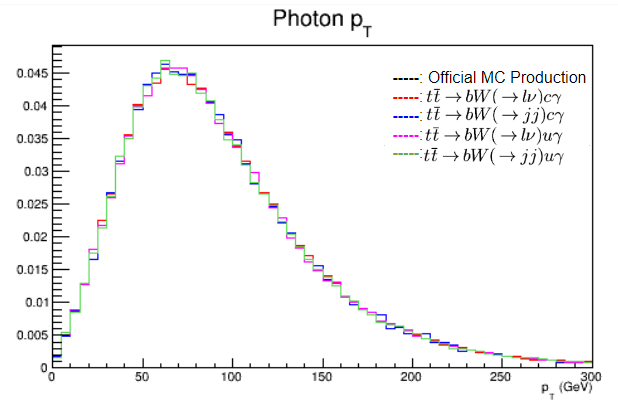
\includegraphics[width=.8\columnwidth]{../ThesisImages/FCNCValidation/photon.png}
	\caption{Normalized $p_T$ of the photons produced by the model for each FCNC final state search and an official $t\bar{t}$ sample, there is 0 contribution from the official $t\bar{t}$ sample.
	}
%	\label{fig:SimMCFlow}
\end{figure}

In the model there are left-and right-handed scalar couplings.  Investigation into differences between the kinematics of the quarks produced using each of these couplings is shown in Figure \ref{fig:LHRHcomp}.
\[ \mathcal{L}_{\gamma t c} = -e \bar{c} \frac{i\sigma^{\mu\nu}q_\nu}{m_t}(\lambda^L_{ct}P_L+\lambda^R_{ct}P_R )t A_\mu + h.c. \]

\begin{figure}[h!]
	\centering
	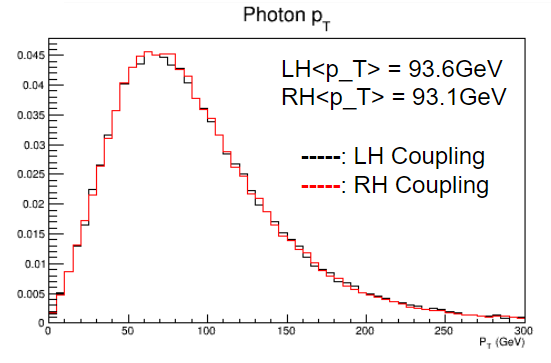
\includegraphics[width=.8\columnwidth]{../ThesisImages/FCNCValidation/PhotonLHRH.png}
	\caption{ Normalized $p_T$ of the photons produced by the model using the Left-handed (LH) and Right-handed (RH) couplings
	}
	\label{fig:LHRHcomp}
\end{figure}

No differences in final state kinematics were shown in the right-handed coupling compared to the left-handed coupling.  Due to this, only one coupling value was used in the production.  In the end only leptonic decays of the W were produced officially.  The leptonic state is simpler to search for than a final state not involving leptons because of the much larger backgrounds from QCD processes.  The lepton offers many handles for searching for these rare FCNC decays.  Using the leptonic final state it is not necessary to use combinatorics for event reconstruction as each object is unique and comes from one particular object.  In this analysis the final state involves a light jet and a photon (from the FCNC decay), and a lepton, photon, and b-jet (from the Standard Model top decay).



%%%%%%%%%%%%%%%%%%%%%%%%%%

\section{Object Reconstruction}

After the events are simulated, or collected in case of real data, the collections of energy deposits within the detector systems must be transformed into meaningful physics objects through reconstruction.  Reconstruction is typically done in two major parts using the specialized detectors covered in Chapter \ref{ch:LHCDetector}.  The Inner Detector and Muon System turn patterns of hits within the tracking detectors into tracks that have direction and momentum information.  The calorimeter system transforms the energy deposits within the calorimeters into calibrated energy deposits with a particular position.  These tracks and calorimeter deposits are used to create physics objects (electrons, muons, etc.) by using particle identification techniques to reconstruct the underlying physics event.  For the analysis presented in this dissertation, the final state signal particles that need to be reconstructed are one lepton (an electron or a muon), one photon, two quarks (one light flavor and one b quark), and one neutrino (missing transverse energy as it is the only particle that does not interact with the detector).  Each of these particles has a particular signature in the subdetectors of the ATLAS detector, shown in Figure \ref{fig:ATLASInteractions}.

\begin{figure}[h]
	\centering
	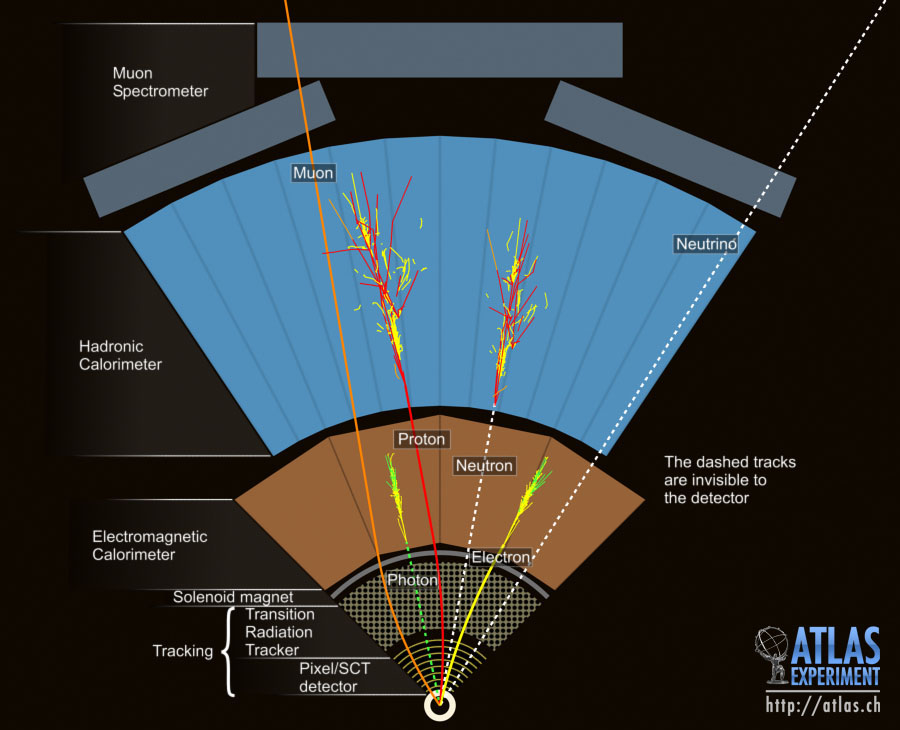
\includegraphics[width=\columnwidth]{../ThesisImages/Simulation/ParticleInteractions.jpg}
	\caption[Cross section of a simulated ATLAS detector showing how various particles interact with ATLAS subsystems.]{Cross section of a simulated ATLAS detector showing how various particles interact with ATLAS subsystems.  Solid lines indicate interactions while dashed lines indicate that no interactions typically occur in that section of the detector. \cite{ParticleInteractions} 
	}
	\label{fig:ATLASInteractions}
\end{figure}


\subsection{Electrons}
Electrons interacting with within the ATLAS detector leave a track in the Inner Detector as well as a cluster of energy in the electromagnetic calorimeter.  The track and cluster are required to be matched together to be identified as an electron candidate\cite{ElectronID}.  As electrons move through the detector they create electromagnetic showers through bremsstrahlung which can produce electron-positron pairs.  The process continues as the particles continue to give energy to the detector.  This collection of electrons, positrons, and photons creates a signature energy cluster in the calorimeter.  

Electron identification algorithms are applied to the electron candidates to separate prompt and isolated electron candidates from electrons that come from backgrounds such as converted photons and misidentified jets.  The electron idenification algorithms use a sliding window ( $3\times5$ in $\eta \times \phi$) in the high granularity section of the LAr electromagnetic calorimeter to search for electron cluster ``seeds'' greater than 2.5 GeV.  Clusters are created around these seeds to form the electromagnetic shower and remove possible duplicate electron signals by containing them within the cluster.  Further pattern recognition for the track fitting allows even larger amounts of energy into the shower to account for bremsstrahlung in the shower shape.  Tracks and clusters are then matched to give electron candidates.  

Electrons coming from background jets or photon conversion are called non-prompt as they do not originate from a signal object/the primary vertex.  In order to reject these electrons, other discriminating variables are used in addition to the track-cluster matching.  These variables inclue the amount of energy leakage into the hadronic calorimeter, thee shower development throughout the electromagnetic calorimeter, and the amount of radiation measured in the TRT.  Three electron identification working points are used: Loose, Medium, and Tight.  Each of these operating points have their own level of background rejection and signal efficiency.  Working points with higher background rejection are a subset of those with lower background rejection.

Isolation variables are another useful tool in the identification of signal electrons from converted photons produced in hadron decays and light hadron misidentification.  These variables are defined by a cone size around the electron candidate and are the sum of the transverse variable (momentum or energy) of all of the tracks within the cone, $p_{T}^{\text{cone0.2}}$ with a cone of $\Delta R =0.2$ (or 10 GeV/$E_T$, for high energy electrons) and $E_{T, Topo}^{\text{varcone0.4}}$ with a cone defined in a similar manner.  

Because the LAr calorimeter is a sampling calorimeter, the energy deposits must be calibrated and scaled such that the true electron energy is read out and not just the small amount of energy deposited into the active layers as discussed in Section \ref{sec:EMHCal}.  The energy scale is calibrated to be uniform throughout the detector.  Any residual differences between data and simulation are corrected.  The calibration strategy was developed for optimal preformance in LHC Run 1\cite{ElectronCalib1} and updated for the conditions of LHC Run 2\cite{ElectronCalib2}.

\subsection{Muons}
Muons behave differently from other particles as they traverse the detector.  They act as minimum-ionizing-particles (MIPs) throughout the calorimeter.  The Muon Spectrometer (MS), Section \ref{sec:MuCal}, specializes in precision measurements of muons.  The Inner Detector (ID) plays a pivotal role in the identification of muons as it offers an independent measure of the muon characteristics.  The muron reconstruction process uses a specific set of variables as well\cite{MuonID}.  These variables include: \textit{ q/p significance}: the difference in the ratio of track charge and momentum measured with the ID and MS, $\rho'$: the difference between the transverse momenta measured with the ID and MS, and $\chi^2$ of the combined track fit using tracks from both the ID and MS.

Muons are separated out into four separate types depending on their interactions with the various subdetectors.  The best muon candidates are combined muons that use hits in the MS to trace back to a track in the ID in order to reconstruct the entire muon track.  Segment-tagged muons are muon candidates that leave a track in the ID but only a segment in the MS instead of a full track.  Segment-tagged muons can occur because of the muon having low $p_T$ or crossing through a region of the MS with reduced acceptance.  Extrapolated muons require only tracks in the MS and are used in regions of $\eta, \phi$ phase space that the ID does not cover.  Calorimeter-tagged muons are muons identified by MIPs in the calorimeters and are used to find muons that cross the ID and MS in regions where cabling might prevent particle detection.

Muons also have their own set of isolation criteria which is track-based $p_{T}^{\text{varcone0.3}}$, with a cone of $\Delta \text{R} = \text{min}(0.3,10\text{ GeV}/p_T)$.  Similar to electrons various working points are available at the analysis level for muons.  These working points are named similarly: Loose, Medium, Tight, and High-$p_T$ in order of background rejection.  

High $p_T$ jets that punch through the hadronic calorimeter can leave tracks in the MS which could be identified as muons.  These would be identified as a bad or a fake muon because of the high-hit multiplicities they leave in the MS as opposed to a single track left by a muon as it is a MIP.  Another source of bad muons is a mismeasured ID track that gets incorrectly matched to segments in the MS.  Fake muons are a source of fake missing transverse energy, $ \slashed{E}_T$

\subsection{Photons}
Photons behave very similarly to electrons in the calorimeter in that they also produce an electromagnetic shower in the calorimeter.  However, they are neutrally charged particles meaning that they should not leave a track in the ID as they do not bend and produce bremsstrahlung photons traveling through the magnetic field.  Prompt photons pair-produce electrons in the tracker, but this process can be identified as the associated cluster in the electromagnetic calorimeter is matched to two tracks with opposite charge.  This process produces what is called a converted photon.  Unconverted photons have no matching tracks associated with an electromagnetic cluster.    

\begin{center}
\begin{table}
\noindent\makebox[\textwidth]{%
\small
{\renewcommand{\arraystretch}{1.6}
\begin{tabularx}{1.25 \textwidth}{ l X lll }
\hhline{=====}
Category 	& Description  & Name  & \textit{loose}  & \textit{tight} \\ \hline
Acceptance 	& $|\eta|<2.37$, with $1.37 \leq |\eta|<1.52$ excluded  & -  &  \checkmark  & \checkmark \\
Hadronic Leakage & Ratio of $E_T$ in the first sampling layer of the hadronic calorimeter to $E_T$ of the EM cluster (used over the range $0.8<|\eta|$ or $|\eta|>1.52$) & $R_{\text{had}_1}$  &  \checkmark  &  \checkmark \\
		&  Ratio of $E_T$ in the hadronic calorimeter to $E_T$ of the EM cluster (used over the range $0.8<|\eta|<1.37$) & $R_{\text{had}}$  &   \checkmark &  \checkmark \\
EM Middle Layer & Ratio of the energy in $3\times 7$ $\eta \times \phi$ cells over the energy in $7\times 7$ cells centered around the photon cluster position & $R_{\eta}$ &   \checkmark &  \checkmark \\
		 & Lateral shower width, $\sqrt{(\Sigma E_{i} \eta_{i}^2 )/(\Sigma E_i )-((\Sigma E_i \eta_i )/(\Sigma E_i))^2}$, where $E_i$ is the energy and $\eta_i$ is the pseudorapidity of cell i and the sum is calculated within a window of $3\times 5$ cells & $\omega_{\eta_2}$ &  \checkmark &   \checkmark\\
		 & Ratio of the energy in $3 \times 2$ $\eta \times \phi$ strips, over the energy of $3\times 6$ cells centered around the photon cluster position  & $R_\phi$ &  &  \checkmark \\
EM Strip Layer & Lateral shower width, $\sqrt{(\Sigma E_i (i-i_\text{max})^2)/(\Sigma E_i)}$, where i runs over all strips in a window of $3 \times 2$ $\eta \times \phi$ strips, and $i_{\text{max}}$ is the index of the highest-energy strip calculated from three strips aroudn the strip with maximum energy deposit & $\omega_{s\text{ 3}}$  &  & \checkmark \\
		 & Total lateral shower width  $\sqrt{(\Sigma E_i (i-i_\text{max})^2)/(\Sigma E_i)}$, where i runs over all strips in a window of $20 \times 2$ $\eta \times \phi$ strips, and $i_{\text{max}}$ is the index of the highest-energy strip measured in the strip layer & $\omega_{s\text{ tot}}$  &  &  \checkmark \\
		 & Energy outside the core of the three central strips but within seven strips divided by energy within the three central strips  & $f_\text{side}$ &  &  \checkmark  \\
		 & Difference between the energy associated with the second maximum in the strip layer and the energy reconstructed in the strip with the minimum value found between the first and second maxima & $\Delta E_s$ &  &   \checkmark \\
		 & Ratio of the energy difference between the maximum energy deposit and the energy deposit in the secondary maximum in the cluster to the sum of these energies & $E_\text{ratio}$ &  &  \checkmark \\
		 & Ratio of the energy in the first layer to the total energy of the EM cluster & $f_1$ &  &  \checkmark \\
\hhline{=====}
\end{tabularx}
\normalsize
}}
\caption[Photon identification variables used for \textit{loose} and \textit{tight} photon identification]{Photon identification variables used for \textit{loose} and \textit{tight} photon identification, taken from \cite{PhotonID}}
\label{tab:PhotonVars}

\end{table}
\end{center}

Prompt photons produce narrower energy deposits in the electromagnetic calorimeter and have smaller leakage into the hadronic calorimeter compared to background photons.  The energy contained within narrow structure in $\eta \times \phi$ strips compared to the energy containd in a larger section can help identify prompt from non-prompt photons \cite{PhotonID}.  Cuts on this and the other variables listed in Table \ref{tab:PhotonVars} are tuned to reduce dependency of identification efficiency on the pileup conditions of Run 2.


\subsection{Jets}

Contrasting with electromagnetic showers produced by electrons and photons, hadronic showers form through QCD processs.  Quarks very quickly undergo showering by emitting gluons which further produce quark-antiquark pairs, analogous to the photons and pair-produced electron-positron pairs of electromagnetic showers.   When quarks have enough energy they hadronize by producing bound states of particles.  These particles are typically pions or mesons that are measured by the ATLAS detector.  The top quark is the only quark that decays before hadronization because it decays so fast ($5\times10^{-25}$ s).  The spray of hadrons coming from a quark from the initial interaction is called a jet and is a collection of detector objects that are traced back and assigned to the quark(s) in the final state of the interaction.  These algorithms are called jet-finding algorithms.  Pictoral representations of the same event reconstructed with four various algorithms is shown in Figure \ref{fig:VarJetAlgs}.

%Ben\cite{CambridgeAachen}
%Ben\cite{JetCleaning}
\begin{figure}[h!]
	\centering
	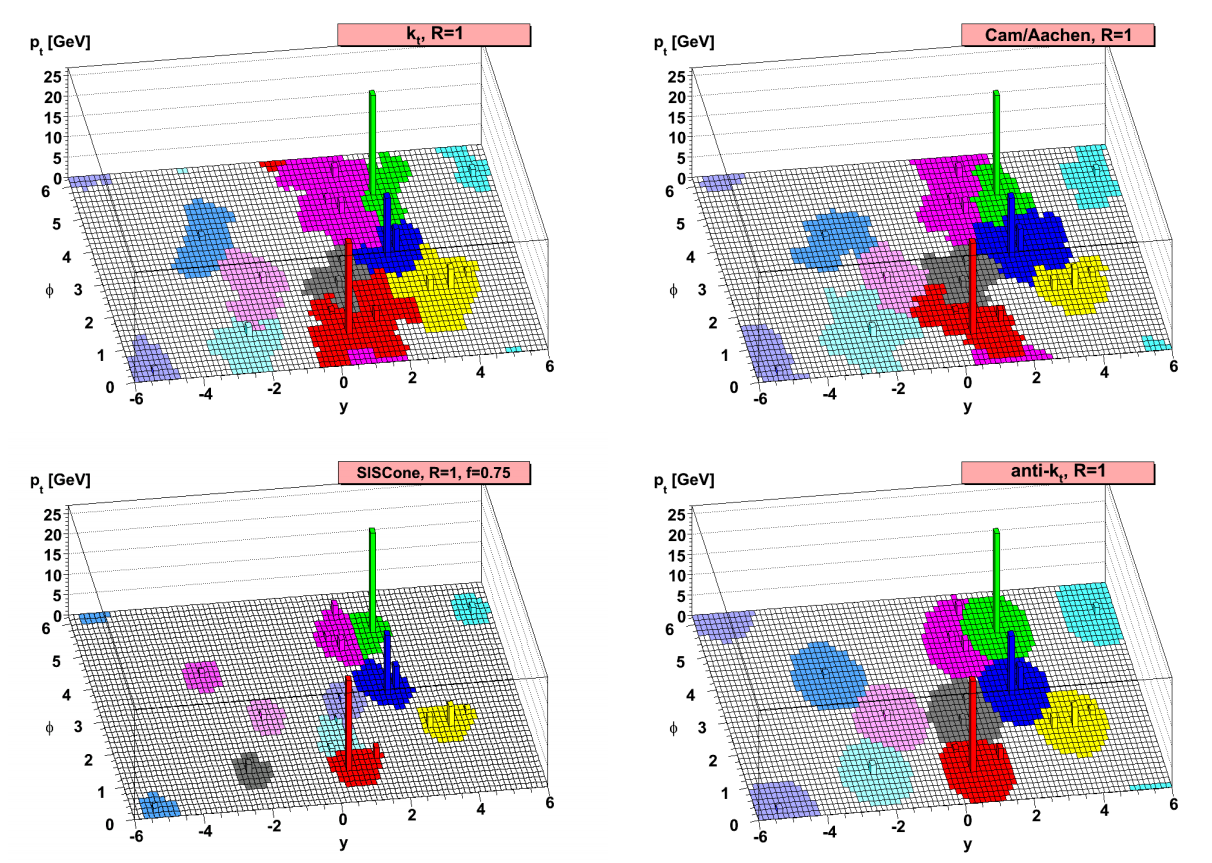
\includegraphics[width=\columnwidth]{../ThesisImages/Simulation/VarJetAlgs.png}
	\caption[A sample parton-level event with many random soft jet objects, clustered with four different jets algorithms, illustrating the areas of the resulting hard jets. For kt and Cambridge/Aachen the detailed shapes are in part determined by the specific set of ghosts used, and change when the ghosts are modified]{A sample parton-level event with many random soft jet objects, clustered with four different jets algorithms, illustrating the areas of the resulting hard jets. For kt and Cambridge/Aachen the detailed shapes are in part determined by the specific set of ghosts used, and change when the ghosts are modified \cite{antikt} 
	}
	\label{fig:VarJetAlgs}
\end{figure}

The jets in this analysis use the anti-$k_T$ algorithm \cite{antikt} with a radius parameter $R=0.4$.  Jets are not physical objects but collections of clustered particles so how they are defined can change the physics objects that are eventually analyzed.  The anti-$k_T$ algorithm is preferred because it is infrared and collinear safe.  Infrared safe jet algorithms do not merge two jets with a soft emission between them.  Adding or removing a soft term between two jets should not change which objects are called jets.  Collinear safe jet algorithms do not change the jet collection if the high transverse momentum particles is split or merged .  Another added benefit of the anti-$k_T$ jet finding algorithm is that it produces roughly circular jet objects, thereby simplifying the calculation of the energy density and simplifying the calibration of the jet object.

The anti=$k_T$ algorithm calculates the distance between an object $i$ and all possible jet objects $j$ ($d_{ij}$) and the beam ($d_{iB}$)
\[ d_{ij} = \text{min}(k_{ti}^{2p},k_{tj}^{2p})\frac{\Delta^2_{ij}}{R},\qquad 
d_{iB} = k_{ti}^{2p} \] 
where $k_{ti}$ is the transverse momentum, $\Delta$ is the distance between the objects, and $p=-1$.  This is a general form for the type of algorithm where the inclusive $k_T$ algorithm has a p value of 1 and the inclusive Cambridge/Aachen algorithm has a p value of 0 \cite{CambridgeAachen}.  The algorithm then follows that if $d_{ij}$ is smaller than $d_{iB}$ then objects $i$ and $j$ are merged, otherwise $i$ is labeled as a jet and removed from the list of entries of possible jet objects.  This is repeated for all entries in the list of possible jet objects.

Jet cleaning is also applied to remove events with jets built from known noisy parts of the calorimeter due to particular calorimeter cells or non-collision background in those areas \cite{JetCleaning}.  To reduce selecting jets that originate from pileup interactions, another requirement on the jet object is made on the jet vertex tagger \cite{JetJVT, JetCleanTwiki} as follows:
\begin{enumerate}
\item For jets with $20 \mathrm{ GeV } < p_{T} < 60 \mathrm{ GeV }$ and $|\eta| < 2.4$: if any jet is bad AND that jet is not marked as pileup by JVT, then reject the event
\item For jets with $20 \mathrm{ GeV } < p_{T} < 60 \mathrm{ GeV }$ and $|\eta| \geq 2.4$: if any jet is bad, then reject the event
\item For jets with $p_{T} \geq 60 \mathrm{ GeV }$: if any jet is bad, then reject the event
\end{enumerate}


\subsubsection{B-Jets}

While jets originate from any quark, jets coming from b quarks can be identified due to their decay products.  B quarks hadronize into b-hadrons which have a relatively long lifetime compared to many other hadrons produced from light quarks.  The longer lifetime and the relativistic speeds at which the hadrons travel mean the particle travels a measureable distance before it decays ($400-500 \mu m$)\cite{CMSct}.  Thus, the vertex reconstructed from the energy coming from a b hadron decay can be traced back to a point that does not correspond to the primary vertex of the event.    A pictoral representation of a b quark decay is shown in Figure \ref{fig:BTagVars}.  The b-jet vertex is called the secondary vertex.  

\begin{figure}[h!]
	\centering
	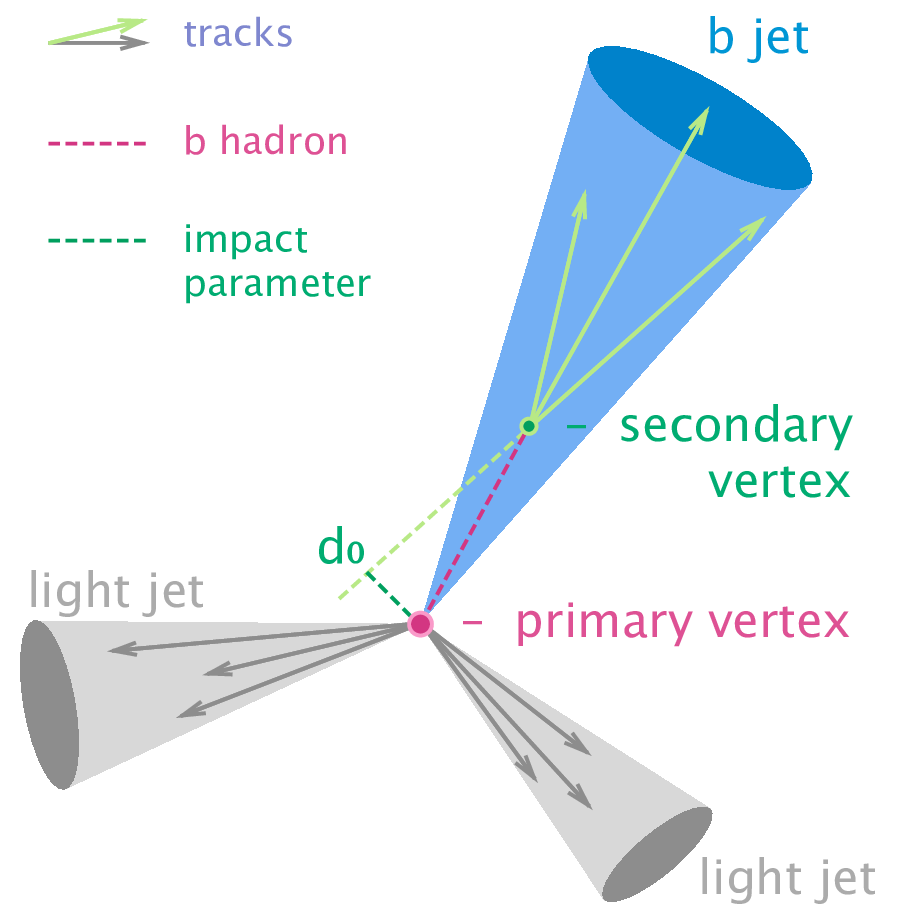
\includegraphics[width=.5\columnwidth]{../ThesisImages/Simulation/B-tagging_diagram.png}
	\caption[Pictoral representation of an event with a b-jet showing the secondary vertex and impact parameter]{Pictoral representation of an event with a b-jet showing the secondary vertex and impact parameter \cite{BTagImg} 
	}
	\label{fig:BTagVars}
\end{figure}

In addition to the secondary vertex, other variables are helpful in identifiying jets coming from b quarks.  By back tracing the tracks within the displaced vertex the minimum distance between the track and the interaction point can be measured, known as the impact parameter.  Reconstructing the decay chain of the jet is also used in determining the providence of the jet.  This information is used in a multivariate analysis (MVA) to identify jets coming from b quarks and reject jets coming from light quarks.

The MVA used in this analysis is the MV2c10, the discriminant used for b-jet identification \cite{BJet1718}.  The output distributions for various flavors of jets as well as background rejection and signal efficiency plots are shown in Figure \ref{fig:BTag}.  The c10 in the algorithm name refers to the background training sample of the MVA consisting of a 10\% fraction of c-jets.  The 77\% efficiency fixed-cut working point for b-jet identification was chosen for this analysis, discussed in Section \ref{sec:NN}.  Differences in efficiency of b-tagging between data and simulation is taken into account with working point specific scale factors provided by the ATLAS Flavour Tagging Combined Performance group.

\begin{figure}[h!]
	\centering
	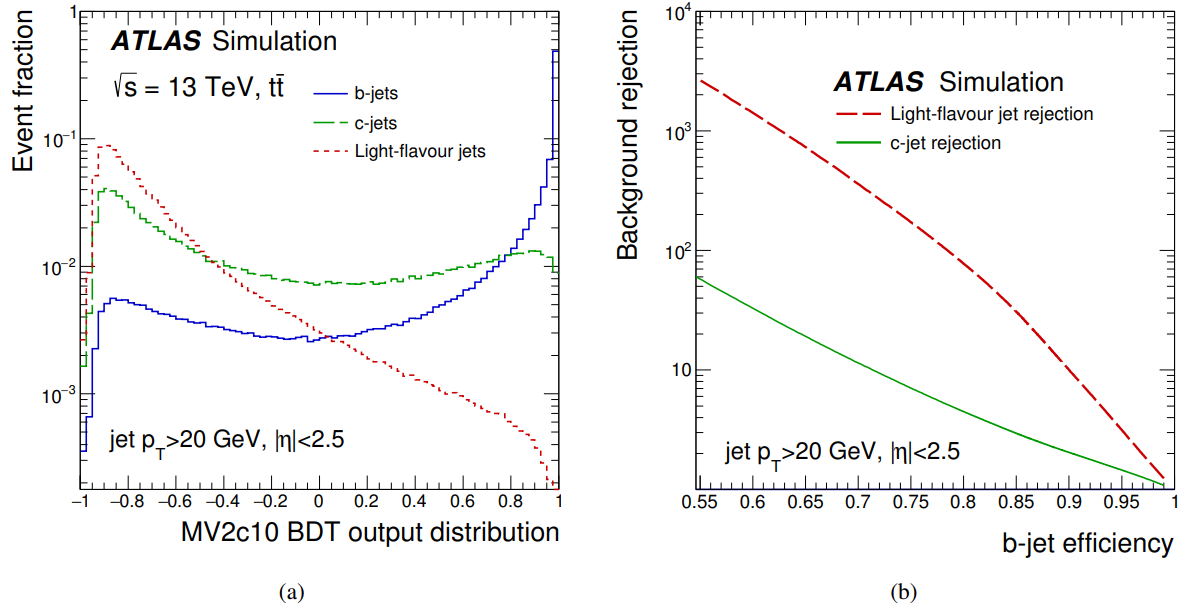
\includegraphics[width=\columnwidth]{../ThesisImages/Simulation/BTagMV2c10andRejVsEff.png}
	\caption[The MV2c10 output for b, c, and light flavored jets in simulated $t\bar{t}$ and the background rejection as a function of the b-jet efficiency]{The MV2c10 output for b, c, and light flavored jets in simulated $t\bar{t}$ and the background rejection as a function of the b-jet efficiency \cite{BJetMVA}
	}
	\label{fig:BTag}
\end{figure}


%\cite{Takubo:2017wvt}%IBL Preformance
\label{sec:bjetReco}

\subsection{Missing Transverse Energy}
The remaining signal object that has yet to be discussed is the neutrino coming from the W boson decay.  Neutrinos do not interact with the detectors as they pass through the ATLAS detector.  The only way to measure any properties of the neutrino in ATLAS events is to use conservation of momentum.  As previously mentioned the collision energy is unknown as partons do not carry a consistent fraction of the beam proton energy.  However, in the transverse plane to the beamline the total momentum is known to be very small.  Before the collision there is on the order of 1 GeV of momentum in the transverse plane.  Therefore, the total transverse momentum of the collision products should be approximately zero.

Any imbalance in the momentum is referred to as Missing Transverse Momentum ($\slashed{E}_T$).  The negative vector sum of all reconstructed objects plus an additional soft term are used to calculate the missing energy in the x-plane and the y-plane\cite{METreco}.  A magnitude and an aziumuthal angle are calculated to give the \textbf{$\slashed{E}_T$} vector in the transverse plane but this does not directly correspond to a neutrino which also has a momentum in the z direction.

\subsubsection{Neutrino Reconstruction}
In this analysis the signal contains only one source of missing energy, therefore all of the missing energy can be used to reconstruct a neturino object.  There is an ambiguity in the choice of the neutrino z-momentum.  To find the z-momentum a $\chi^2$ minimization is done:
\[ \chi^2 = \chi_{\text{SMTop}}^2 + \chi_{\text{W}}^2 \]
\[ \chi^2 = \frac{(m_{\text{bjet},l,\nu}-m_t)^2}{\sigma_{\text{SMTop}}^2} + \frac{(m_{l,\nu}-m_W)^2}{\sigma_W^2} \]
The widths $sigma_{\text{SMTop}}$ and $\sigma_W^2$ are determined from signal Monte Carlo.  The event objects are combined to calculate the invariant mass of the top quark (the combination of the b-jet, lepton, and neutrino) and the W boson (combination of the lepton and neutrino).  The $\chi^2$ minimization is is done while varying the z-momentum of the neturino.  The neutrino momentum that corresponds to the smallest $\chi^2$ value is given assigned to the neutrino object for further use in the analysis.  The $\chi^2$ values are also used as a discriminating variable and fed into a neural network (Section \ref{sec:NN}).







         

\chapter{Search Strategy}
\label{ch:SearchStrategy}
%Deep thoughts go here.
This chapter will describe the major backgrounds and outline a search strategy used in the analysis.  The kinematic regions for the signal will be defined as well as the introduction of neural networks to assist with the separation of signal and background-like events.  This chapter contains material coauthored with the ATLAS Collaboration.  I developed the signal samples and analysis framework, optimized the signal regions, and was responsible for the the background modeling in the regions shown here including the fake rate studies.  Other members of the ATLAS Collaboration developed the background samples used to produce the results presented in this chapter.


\section{Major Backgrounds}
There are a large number of Standard Model processes that can end up in the signal region and share a similar final state topology as the studied signal process, $t\bar{t}\rightarrow b l \nu q \gamma$.  All of these processes are modeled with Monte Carlo (MC) simulation, with the exception of particles that fake other particles (leptons and photons) which are done using data-driven techniques because they are poorly modeled with MC.  A full list of the Monte Carlo samples used for each background can be found in Appendix \ref{app:MC_Samples}. 

The dominant backgrounds in this search are Standard Model $t\bar{t}$ and Standard Model $t\bar{t}+\gamma$, as well as W+jets and W+jets with an associated photon (W+jets+$\gamma$).  These, along with minor backgrounds (Standard Model single top events, Z+jets (Z+jets+$\gamma$), $t\bar{t}$+Vector Boson, diboson), are all modeled with MC and some data-driven estimates and corrections are applied.  The various backgrounds modeled in this search are summarized here:

\begin{description}
\item[\textbf{SM Processes}:]  SM $t\bar{t}$, W+jets, Z+jets, single top, diboson, $t\bar{t}$+V are modeled with MC simulations.  Control and validation regions are designed to test performance of the largest of these background proceses, $t\bar{t}$ and W+jets.  A discussion of the modeling of the major SM processes without photons and a derivation of additional scale factors for these processes are in Section \ref{sec:BKGnoPho}.

\item[\textbf{SM Processes with an associated photon}:] SM + associated photon processes $t\bar{t}+\gamma$, W+jets+$\gamma$, and Z+jets+$\gamma$ are modeled with MC simulation and overlap removal is applied to the SM processes to remove events with similar phase spaces since these processes are a subset of the SM process.  MC simulations are created with additional statistics for these processes.  Further details are presented in Section \ref{sec:BKGPho}.

\item[\textbf{Fake Leptons}:] Non-prompt or fake electrons and muons can arise from semi-leptonic decay of $b$ and $c$ quarks.  For electrons additional contributions from photon conversions and jets in the electromagnetic calorimeter can lead to lepton fakes.  Muons can be faked via energetic showers in the hadronic calorimeter or from hadrons that punch through the hadronic calorimeter.  The matrix method is used to estimate the number of events with fake leptons as described in Section \ref{sec:FakeLep}.

\item[\textbf{Fake Photons}:] The number of events with fake photons is estimated using a $Z\rightarrow e^+ e^-$ tag-and-probe method discussed in Section \ref{sec:FakePho}.  Further, the ABCD method is used in Section \ref{sec:FakePho2} to estimate the number of fake photon events that arise from a jet faking a photon.  

\end{description}
\subsection{Overlap Removal}
\label{sec:OverlapRemoval}
Tracks and energy deposits within the detector can, in some cases, be used to reconstruct multiple objects.  To prevent using these tracks and deposits multiple times a standard overlap removal procedure is applied to objects.  First, electrons that share tracks with any other electrons are removed.  Any electron sharing a track with a muon is then also removed.  Any jet that is found within  $\Delta R < 0.2$ of an electron is removed.  Then any jet with fewer than three tracks associated with it within $\Delta R < 0.2$ of a muon object is removed.  After that any muon found withing $\Delta R < 0.4$ of a jet is removed and any photon within $\Delta R < 0.4$ of an electron or muon object is removed. % Any jet found within $\Delta R < 0.4$ of a \textit{Loose} photon is also removed. 

\subsection{Duplicate Event Removal}
As specialized higher statistic samples are used for processes with prompt photons, a double counting of events could occur with the nominal MC samples.  For example, in addition to the $t\bar{t}$ sample a sample of $t\bar{t}+\gamma$ events are used.  This is true for the W+jets/Z+jets and special samples of W+jets+$\gamma$ and Z+jets+$\gamma$.  Therefore a truth-based matching scheme is used to remove events in the nominal samples that match with the photon types produced in the specialized $+\gamma$ samples, i.e., they contain a truth photon that does not originate from a hadron or lepton.

\section{Event Selection}
This analysis is searching for $t\bar{t}$ candidate events where one of the top quarks decays through the most common decay path (a W boson that decays leptonically to an electron or muon and a bottom quark) and the other through the FCNC diagram to an up-type light quark and a photon.  The selected decay path is then $t\bar{t} \rightarrow Wbq\gamma \rightarrow l\nu b q \gamma$ such that the final state will contain at least two jets, exactly one of which is b-tagged using the MV2c10 algorithm, exactly one lepton (an electron or muon), exactly one highly energetic photon, missing transverse energy from the neutrino, and a large transverse W mass.  The transverse W mass requirement selects events that have a lepton and $\slashed{E}_T$ which are consistent with a leptonically decaying W boson, defined as:
\[ m_T^{W} =  \sqrt{2\times p_{T_l}\times \slashed{E}_T \times (1 - \text{cos}(\phi_l -\phi_{\text{MET}}))}\]
which is largest when the lepton and missing transverse energy are close in $\phi$ as would be expected from the decay products of a boosted W boson.  Events are selected loosely to include all possible kinematic regions of interest and then skimmed down to the individual regions for various studies.  This includes events that will not enter the signal region such as events with 0 photons or events with 0 b-jets that are used to derive and test scale factors on the largest background samples and account for mismodeling of MC simulations. 

For the events that have a chance of entering the final Signal Region, i.e., events with exactly one b-tagged jet and exactly one photon, a neural network analysis is performed to help separate the signal from the background using a variety of high dimensional cuts.  The neural network training and testing are described in Section \ref{sec:NN}.  The neural network is then applied to all events with exactly one b-tagged jet and one photon and greatly increases signal purity while separating out the most dominant backgrounds, in particular $t\bar{t}$ and $t\bar{t}+\gamma$.




%%%%%%%%%%%%%%%%%%%%%%%%%%%%%%%%%%%%%%%%%%%%%%
%%%%%%%%%  									        	 %%%%%%%%
%%%%%%%%%                     Start of Neural Net Section                                           %%%%%%%%
%%%%%%%%%										 %%%%%%%%
%%%%%%%%%%%%%%%%%%%%%%%%%%%%%%%%%%%%%%%%%%%%%%

\section{Event Classification: Neural Network Optimization}
\label{sec:NN} 
To help distinguish signal events from the majority of background events, neural networks were employed for event classification.  Neural networks are multivariate methods that take a variety of inputs and output a number between 0 and 1.  The output value is a discriminating variable that will be used to classify events and determine which events make it into the final Signal Region selection.  Signal-like events accumulate towards 1 while background-like events cluster around 0.  Two neural networks are trained, one for the electron+jets final state and one for the muon+jets final state.  This section will discuss the neural network studies completed and their uses in the search for FCNC events.  

\subsection{Input Variables}
A wide variety of input variables to the neural network were studied in detail.  Studies were done using only low-level variables such as the kinematic variables  ($p_T$, $\eta$, $\phi$, $E$)  of the physics objects in the signal region. While a complex enough neural network should be able to figure out useful high-level/event-level variables (i.e., invariant masses, geometric separations), in practice a combination of some of these low-level variables and high-level variables used as inputs to the neural network proved to give the best separation and projected limits.  Using physical intuition to guide the neural network proved to be a valuable tool.

Combinations of 29 input variables were tested at the outset.  However, variables such as $\eta$ and $\phi$ tend to not have significant weights in the neural network and are left out in favor of the high-level variables that include them (e.g., $\Delta R$ values).  A measure of how different the variables are between signal and background is the separation.  Table \ref{tab:Separations} shows the separation values for the variables that are inputs to the final neural network.  Comparisons between the shapes of the input variables for the $\mu$+jets channel are shown in Figures \ref{fig:VarPlots1}, \ref{fig:VarPlots2}, and \ref{fig:VarPlots3}.

\begin{table}[]
\begin{center}
{\renewcommand{\arraystretch}{1.2}
\begin{tabular}{ccc}
\hline
Variable  &  Separation e+jets   & Separation $\mu$+jets   \\  \hline 
$p_T (\gamma)$            &  22.97   & 24.01	\\
$m_{q\gamma}$           &   22.65 &  28.31	\\
$\gamma_{\text{iso}}$   &  18.62   &  41.32	\\   
$m_{bW} $                    &  11.10   &  11.70 	\\
$m_{l\gamma}$             &  9.00  &   7.51	\\
$\Delta R_{j\gamma}$ &  4.59   &  5.66	\\
$\Delta R_{b l}$            &  4.99   &  4.47 	\\
$m_{T}^{W}$              &   3.16  &   3.37	\\
$S_T$                            &  3.78   &  3.32 	\\
$n_{\text{jets}}$         &  1.70   &   2.03	\\
$\chi^{2}_{W}$           &  1.37 &   1.91	 	\\
$p_T (q)$                      &  2.46    &  2.82	\\
$\Delta R_{l \gamma}$ &   1.40 &  1.19		\\
E (lepton)                       &  0.86  &  0.89	\\	
$\slashed{E}_T  $          &   0.47  & 0.70 	\\
$p_T (b)$                       &  0.51    &  0.53	\\ \hline
\end{tabular}
\caption{Separation of normalized variables between signal and background in the e+jets and $\mu$+jets channels for the variables used as input to the final neural network.  }
\label{tab:Separations}
}
\end{center}
\end{table}

\begin{equation}
 \text{Separation} = \sum_{i}^{bins} \frac {(n_{s i}-n_{b i})^2}{n_{s i}+n_{b i}}
\end{equation}

Signal and background distributions are normalized separately to one for the calculation of the separation.  The backgrounds are pre-normalized with the process cross sections such that the relative representation of each background is accurate to the final distributions of the analysis.

Typically the kinematic variables with photon information have the biggest separation values.  This is expected because the signal photon comes directly from the decay of a top quark and is much more energetic than background photons.  Shape comparison plots for the $e$+jets channel and additional plots for other investigated variables are shown in Appendix \ref{app:NN}.  The largest difference in separation between the $e$+jets and $\mu$+jets channels is the photon isolation value.  This is due to the fact that all backgrounds are included and fake photon contamination from a large Z+jets background is expected.  Both networks perform similarly in their separation of signal and background events.  The network is able to learn and compensate for this behavior with the help of other variables that include the lepton and photon: $\Delta R_{l \gamma}$ and $m_{l\gamma}$.

The neural networks are trained on MC events that have a chance of being in the signal region after basic event-level cuts and are optimized for signal significance.  Only events with one photon ($>15$ GeV) and one b-jet (MV2c10 77\% working point) are classified by the neural network.  The 77\% working point was chosen by training the neural network on events with only one b-jet at each working point: 70\%, 77\%, and 85\%, and picking the network and working point with the best estimated significance.  The b-tagging neural network study is shown in Section \ref{sec:btagNN}.

\begin{figure}[h!]
\centering
\subfloat[$\gamma_{iso}$ topo$E_{T}$cone40]{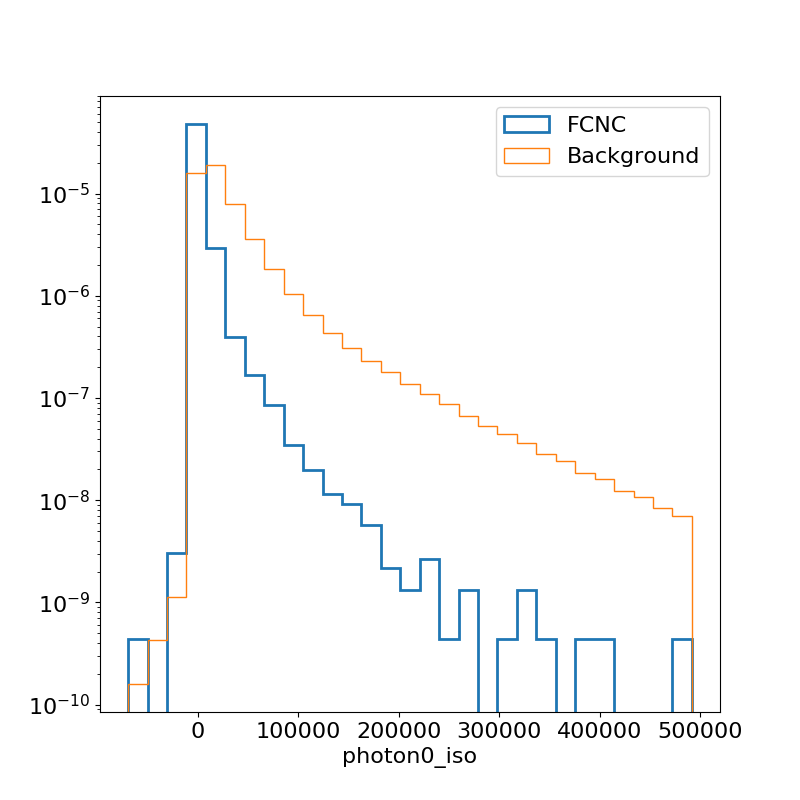
\includegraphics[width=.4\columnwidth]{../ThesisImages/SearchStrategy/varplots/photon0_iso.png}}\hfil
\subfloat[$\gamma_{p_T}$]{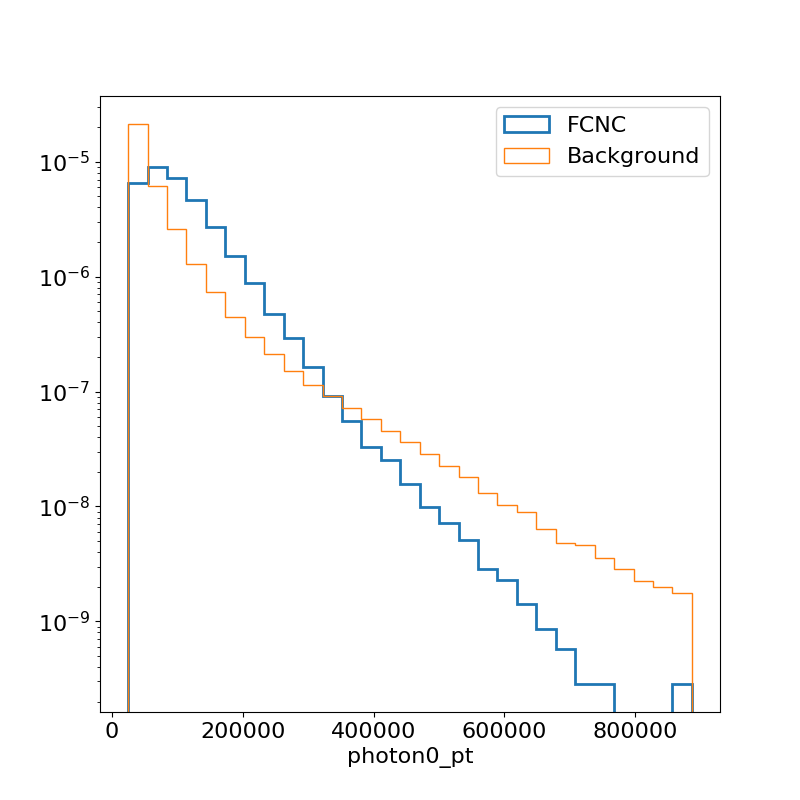
\includegraphics[width=.4\columnwidth]{../ThesisImages/SearchStrategy/varplots/photon0_pt.png}}
\vspace{-4.5mm}
\subfloat[$m_{q \gamma}$]{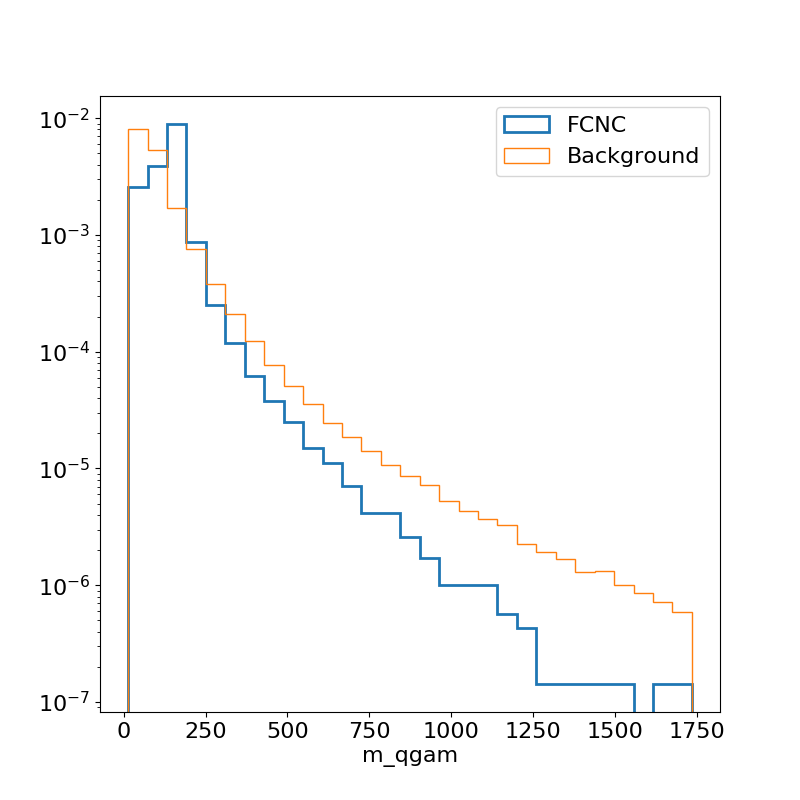
\includegraphics[width=.4\columnwidth]{../ThesisImages/SearchStrategy/varplots/m_qgam.png}}\hfil
\subfloat[$m_{l \gamma}$]{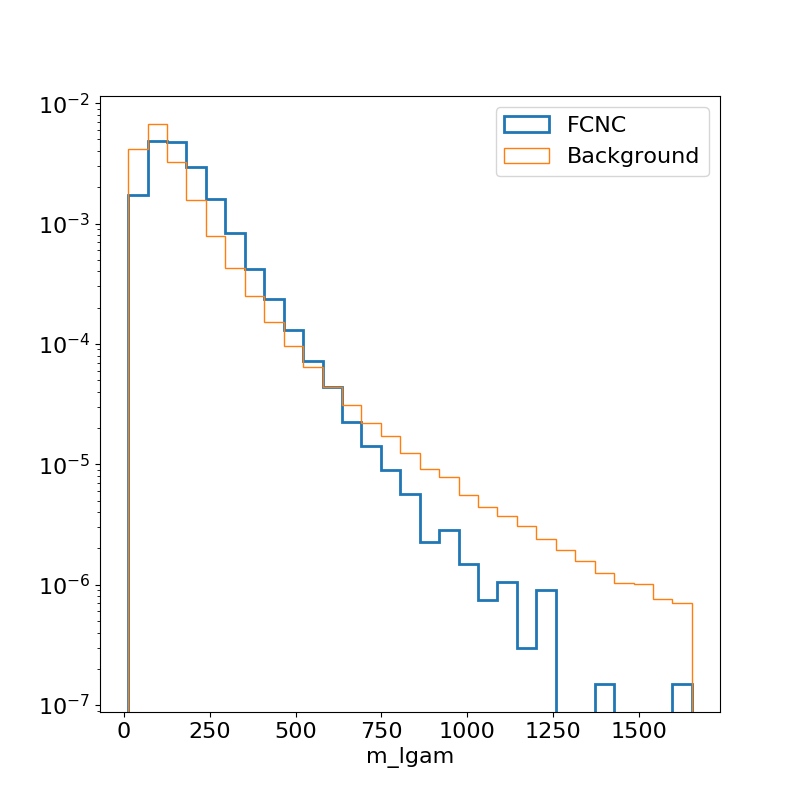
\includegraphics[width=.4\columnwidth]{../ThesisImages/SearchStrategy/varplots/m_lgam.png}}   
\vspace{-4.5mm}
\subfloat[$m_{bW}$]{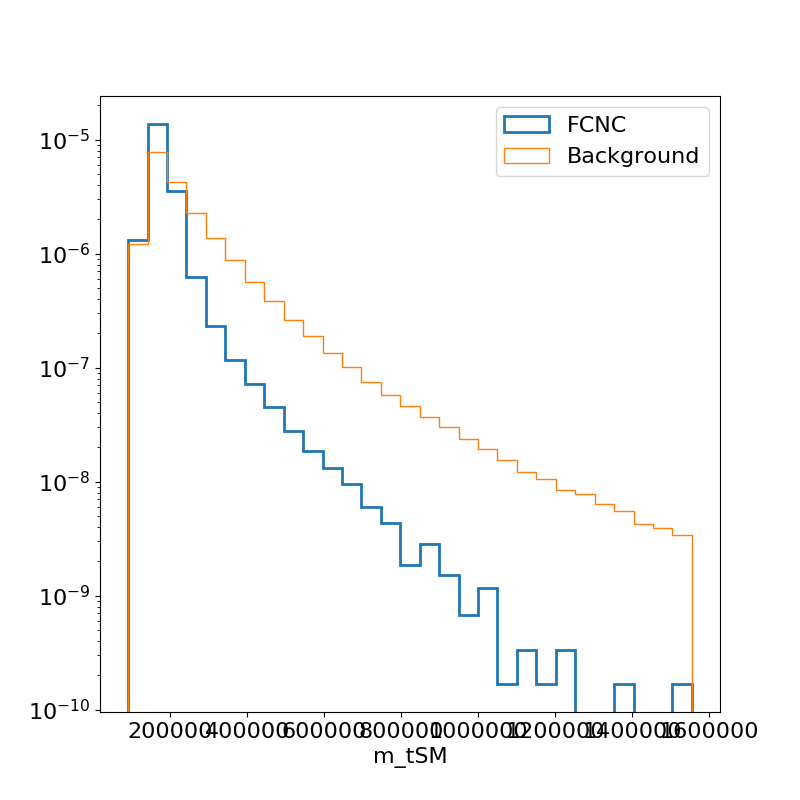
\includegraphics[width=.4\columnwidth]{../ThesisImages/SearchStrategy/varplots/m_tSM.png}}\hfil
\subfloat[$\Delta R_{j\gamma}$]{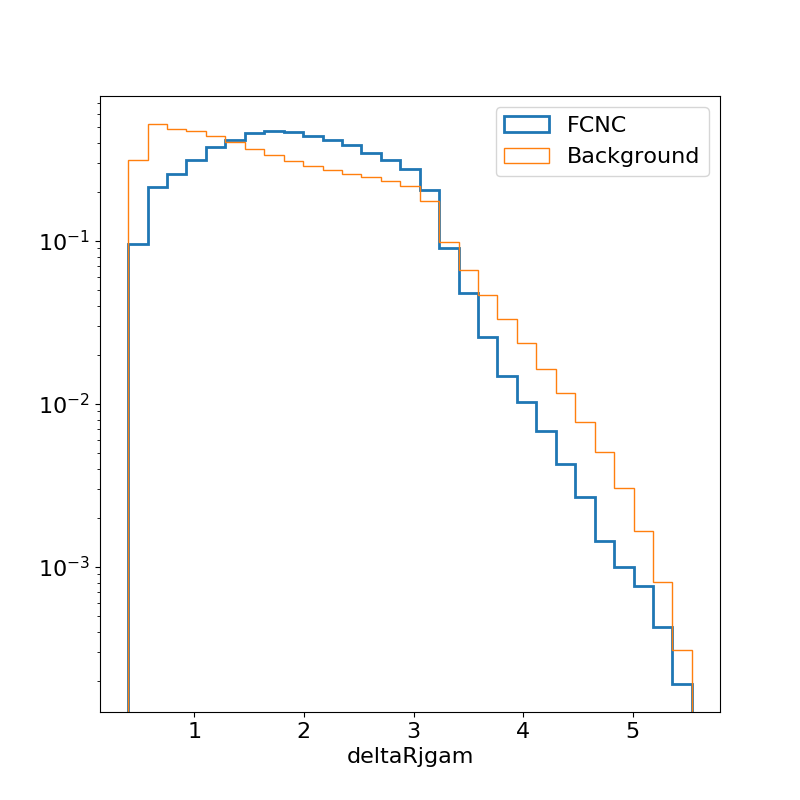
\includegraphics[width=.4\columnwidth]{../ThesisImages/SearchStrategy/varplots/deltaRjgam.png}}
\caption{Normalized variables showing the shapes of neural network input variables for the $\mu$+jets channel: $\gamma_{iso}$ topo$E_{T}$cone40, $\gamma_{p_T}$, $m_{q \gamma}$, $m_{l \gamma}$, $m_{bW}$, and $\Delta R_{j\gamma}$. }
\label{fig:VarPlots1}
\end{figure}



\begin{figure}[h!]
\centering
\subfloat[$\Delta R_{b l}$]{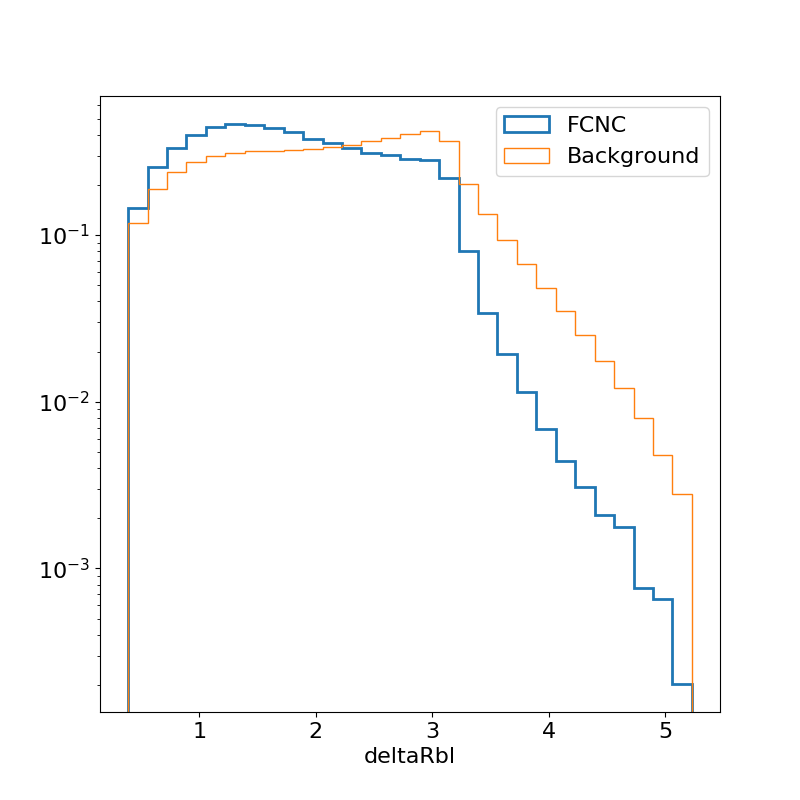
\includegraphics[width=.4\columnwidth]{../ThesisImages/SearchStrategy/varplots/deltaRbl.png}}\hfil
\subfloat[$m_{T}^{W}$ ]{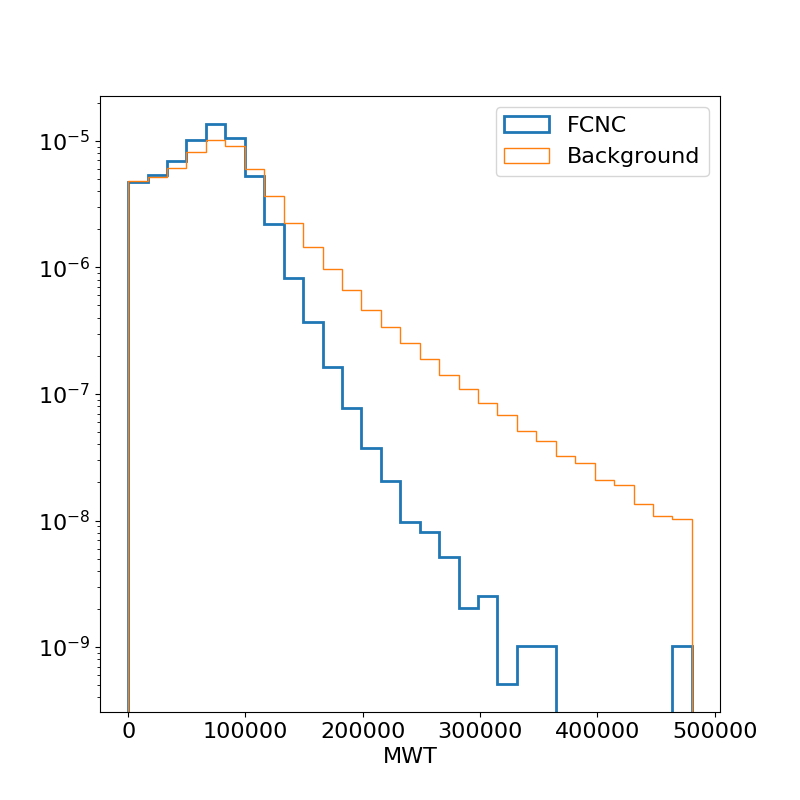
\includegraphics[width=.4\columnwidth]{../ThesisImages/SearchStrategy/varplots/MWT.png}}
\vspace{-4.5mm}
\subfloat[$S_T$]{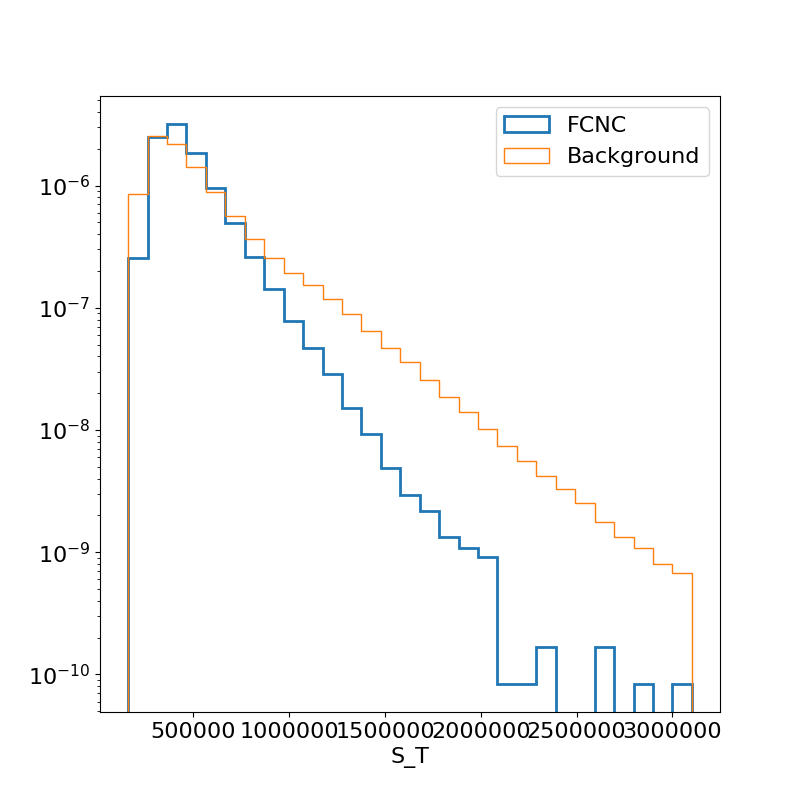
\includegraphics[width=.4\columnwidth]{../ThesisImages/SearchStrategy/varplots/S_T.png}}\hfil
\subfloat[$n_{\text{jets}}$]{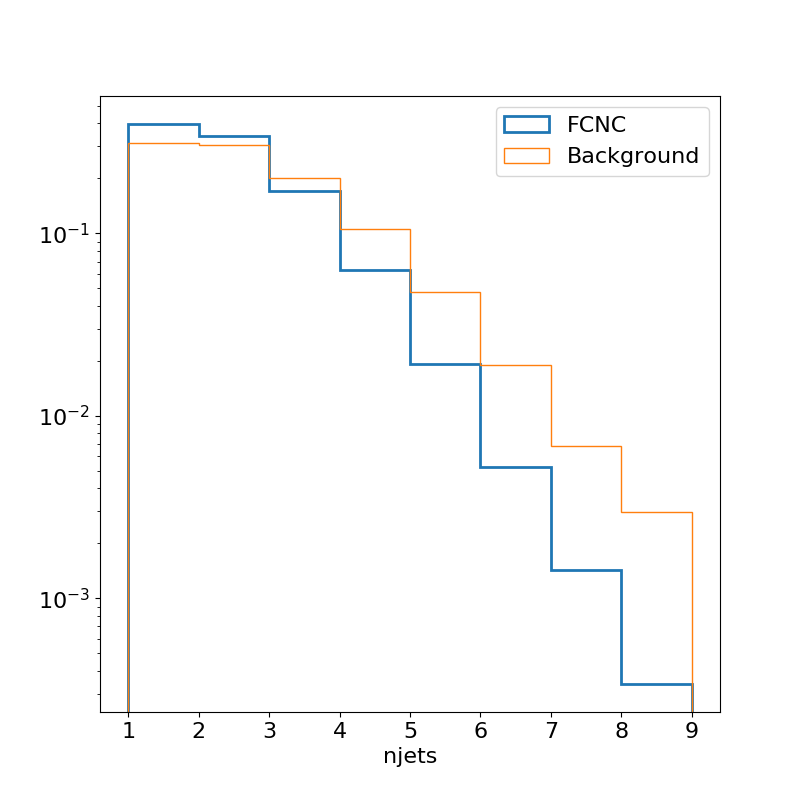
\includegraphics[width=.4\columnwidth]{../ThesisImages/SearchStrategy/varplots/njets.png}}   
\vspace{-4.5mm}
\subfloat[$\chi^{2}_{W}$]{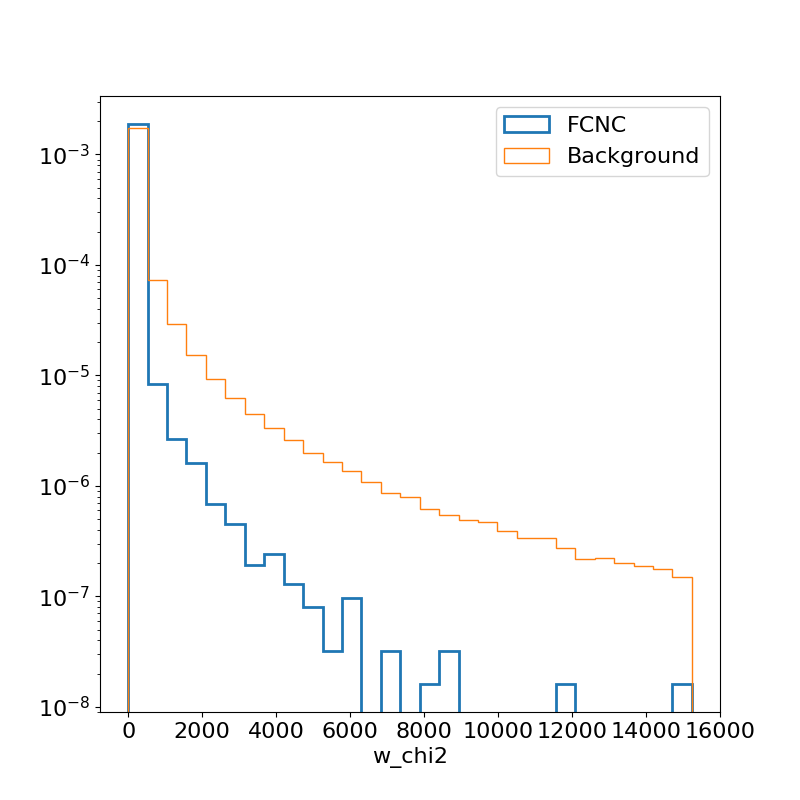
\includegraphics[width=.4\columnwidth]{../ThesisImages/SearchStrategy/varplots/w_chi2.png}}\hfil
\subfloat[$p_T (q)$]{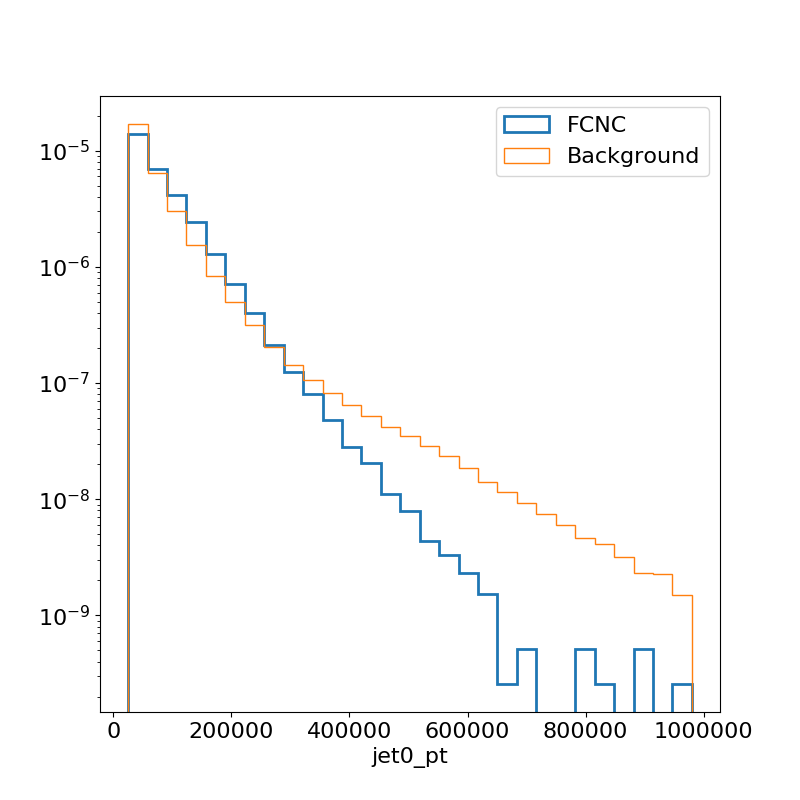
\includegraphics[width=.4\columnwidth]{../ThesisImages/SearchStrategy/varplots/jet0_pt.png}}
\caption{Normalized variables showing the shapes of neural network input variables for the $\mu$+jets channel: $\Delta R_{b l}$, $m_{T}^{W}$ , $S_T$, $n_{\text{jets}}$, $\chi^{2}_{W}$, and $p_T (q)$.}
\label{fig:VarPlots2}
\end{figure}

\begin{figure}[h!]
\centering
\subfloat[$\Delta R_{l \gamma}$]{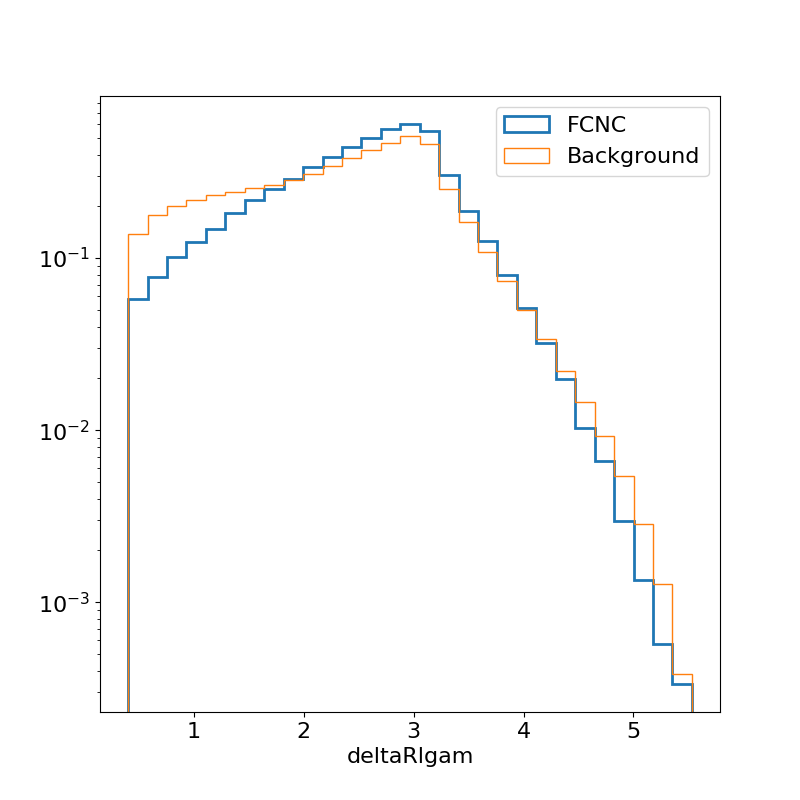
\includegraphics[width=.4\columnwidth]{../ThesisImages/SearchStrategy/varplots/deltaRlgam.png}}\hfil
\subfloat[E (lepton)]{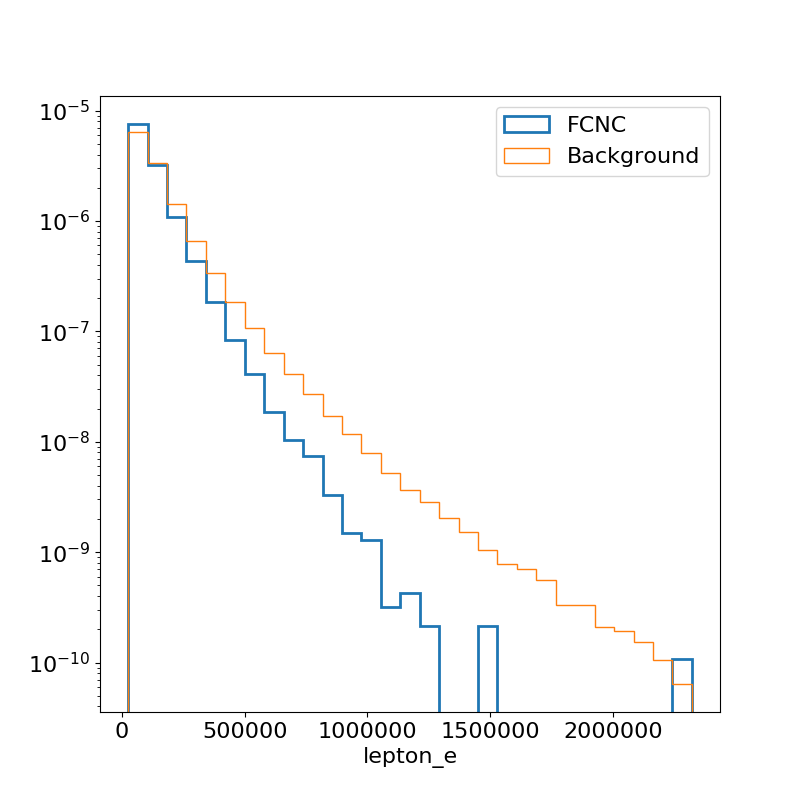
\includegraphics[width=.4\columnwidth]{../ThesisImages/SearchStrategy/varplots/lepton_e.png}}
\vspace{-4.5mm}
\subfloat[$\slashed{E}_T  $]{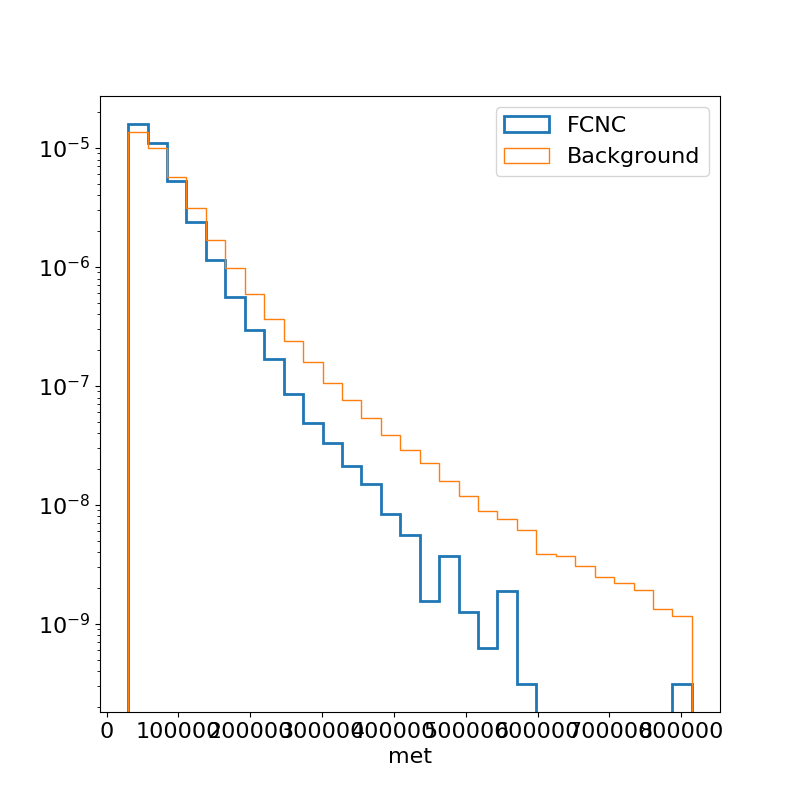
\includegraphics[width=.4\columnwidth]{../ThesisImages/SearchStrategy/varplots/met.png}}\hfil
\subfloat[$p_T (b)$ ]{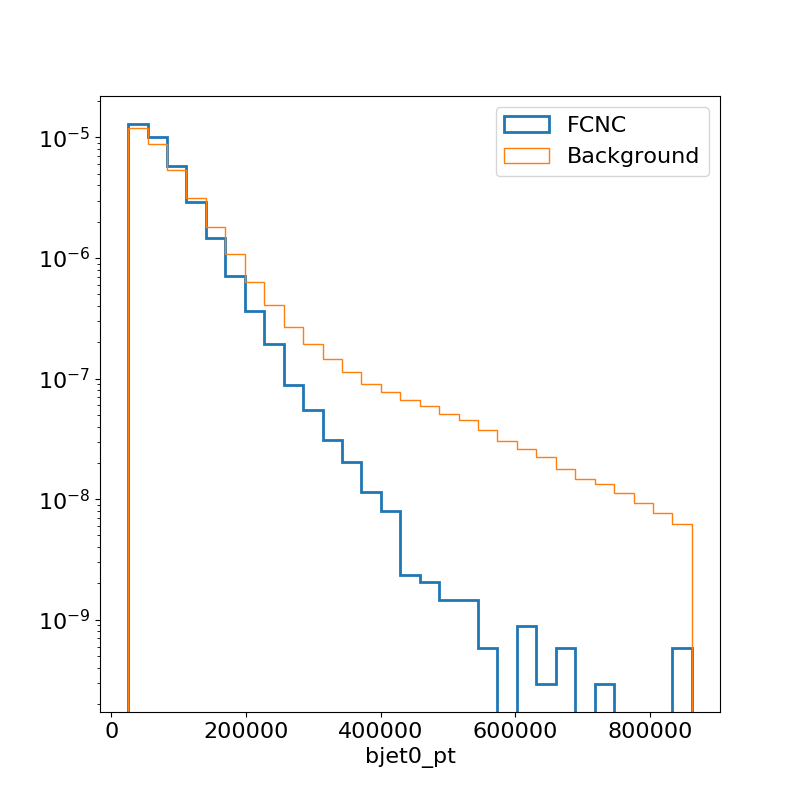
\includegraphics[width=.4\columnwidth]{../ThesisImages/SearchStrategy/varplots/bjet0_pt.png}}   
\caption{Normalized variables showing the shapes of neural network input variables for the $\mu$+jets channel: $\Delta R_{l \gamma}$, E (lepton), $\slashed{E}_T  $, and $p_T (b)$.}
\label{fig:VarPlots3}
\end{figure}


\subsection{Architecture}

A variety of architectures of dense neural networks are studied using \textsc{Keras}\cite{Keras} on top of the \textsc{TensorFlow} backend\cite{TensorFlow}.  Each network has a number of input nodes equal to the number of input variables.  Networks with one, two, and three hidden layers are investigated each with 20 nodes.  The output layer contains only a single node.  Every node in one layer is connected to every node in the next layer and the previous layer.  Every connection is assigned a weight that is optimized during the training of the network.  For every node in the network a value is computed using the weights and input values of the previous nodes using an activation function.  Nodes with the highest output of this function are more important to the fit.  The activation function used on the internal nodes in this search is the Rectified Linear Unit activation function.
\[ ReLU(x) = 
\begin{cases}
x, \qquad \text{if } x \geq 0\\
0, \qquad \text{if } x < 0
\end{cases}
\]
The output layer uses the sigmoid function, $\sigma(x)$, as an activation function.  The sigmoid function maps the output smoothly to the range (0,1).
\[ \sigma(x) = \frac{1}{1+e^{-x}}
\]
In every training step the weight of each node is updated following an optimization algorithm, in this case the \textsc{Adam} optimizer\cite{AdamOpt}.  This optimizer follows the steepest gradient to reach the minimum of the parameter of interest called the loss function.  The loss function used for these classification neural networks is the binary cross entropy:
\[\text{Loss} = -\frac{1}{N}\sum_{i=1}^{N}y_{i} \text{log}(p(y_{i}))+(1-y_{i})\text{log}(1-p(y_{i}))\]
where $y$ is a binary indicator (0 or 1) if class label is the correct classification for observation and $p$ is the predicted probability observation of the class label (0 or 1).  The logarithmic nature of this loss function means it applies small values to correctly assigned events but more harshly punishes mismatching of events.  Therefore, having a similar number of signal and background events that get weighted similarly can improve the behavior of the network.  In rare decay searches typically the number of signal events is significantly smaller than the number of background events in the training sample.  By using the weight functionality in \textsc{Keras}, the total number of signal events can be scaled to be similar to the number of background events. 

Weighting the signal events this way allows the network to separate the signal and background events in a way that is significantly less harsh than without the weights by taking advantage of the loss function being used.  This improves the estimated significance of the neural network cut after the signal events are rescaled to their proper normalization values.  

\begin{figure}[h!]
	\centering
	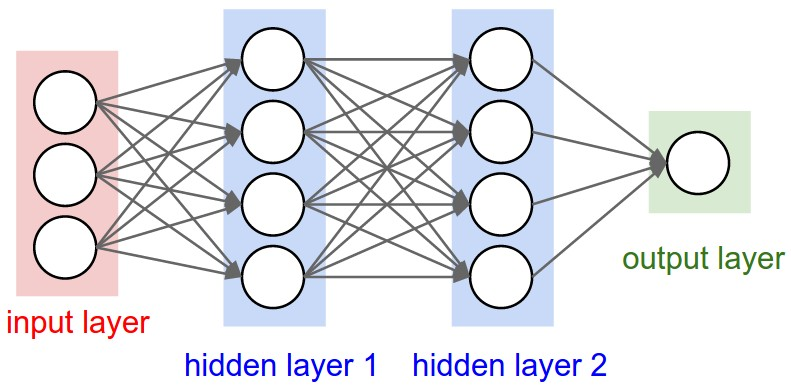
\includegraphics[width=\columnwidth]{../ThesisImages/SearchStrategy/neural_net2.jpeg}
	\caption[Pictoral representation of neural network architecture with three input variables, two hidden layers with four nodes each, and one output layer.]{Pictoral representation of neural network architecture with three input variables, two hidden layers with four nodes each, and one output layer\cite{NNImage}.}
	\label{fig:NNArch}
\end{figure}

Various hyperparameters are used as inputs into the neural network as well as the optimizer used.  The \textsc{Adam} optimizer has a default learning rate of 0.001 which remained constant throughout these studies.   The learning rate corresponds to the amounts by which weights are updated during training.  A learning rate that is too large can mean the network never settles into a local minima as it is always missing the minima or, at the very least, it can take much longer to converge into a minima.  As the neural network training for this search always converged quickly and to a similar value after being tested multiple different times, the learning rate was not adapted.  

Another hyperparameter of note is the batch size that defines the number of samples that are propagated through the network at once.  The batch size is crucial in determining how long the training of the network takes.  A set of 1000 training samples with a batch size of 100 will propagate each set of 100 samples through the neural network every epoch, meaning 10 separate batches.  A larger batch size means that each epoch of the training takes a shorter amount of time.  However, as the weights are updated after each batch, the network can take many more epochs to converge as the weights are being updated less frequently.  A batch size of 100 was used while training the networks presented in this chapter.  Larger batch sizes were tested with the only difference being the time each epoch took and the total time the network took to converge.

Epochs are the total number of times the network is trained over the entire training set.  All of the networks are allowed up to 200 epochs to converge with a \textsc{Keras} patience value set to 50.  The loss function minimization is done every batch, and after each epoch the best possible value of the loss function is found.  If this value is better than any previous epoch the network is allowed to train for 50 more epochs until 50 epochs have passed without finding a new minimum loss function value which then terminates the training.  All models converge early and are terminated typically between epoch 80 and 120, meaning the loss function was minimized between epoch 30 and 70.  

One method employed to avoid overtraining the network is to use dropout regularization on each of the hidden layers.  Dropout has the effect of simulating a large number of networks with very different network structures by removing nodes randomly throughout the training. A dropout rate of 20\% is used, meaning that for every batch 20\% of the weights of the hidden layer nodes are set to 0.  This prevents the network from becoming overly dependent on any given node or learning the data `by heart' as opposed to recognizing the trends in the sample. 

\subsubsection{Training and Validation of Neural Networks}

The input variables into the neural network are preprocessed using the \textsc{RobustScalar} method implemented in \textbf{scikit-learn}\cite{ScikitLearn}.  The preprocessing is done so that the input variables exist on a similar scale.  As the network is tasked with learning how to combine these inputs through a series of linear combinations and nonlinear activation function values, a disparity in the scales of the input values can lead to awkward loss function topology that focuses on certain parameter gradients instead of treating them all similarly.  Normalizing the values to a standard scale allows the network to learn the optimal parameters for each input node more quickly and efficiently.  This means that less focus can be used on the optimization of the hyperparameters for the network as the scales of the inputs do not need to be learned by the network itself.

Each input variable in the neural network, $x$, is scaled by the following equation:
\[ z = \frac{x - m }{q_3 - q_1} \]
where $m$ is the median of the distribution, and $q_1$ and $q_3$ are the first and third quartile.  This changes the distribution of the input variable distributions to be centered around zero.

A second method to avoid overtraining the neural network is to make use of a train-test split to split the signal and background samples into three independent randomized sets before training the neural network.  The samples are split into a training set of 64\% of the samples and a test set  containing 20\% of the samples, and the remaing 16\% are a validation set.  The training and test sets are used during the training of the network while the validation set is used to compute performance of the trained neural network.

One measure of the performance of the network is the accuracy. The \textsc{Keras} default accuracy measure is defined:
\[ \text{accuracy} = \frac{N(\text{event}_{NN} \geq 0.5|\text{signal})+ N(\text{event}_{NN} <0.5|\text{background})}{N(\text{signal})+N(\text{background})} \]
where $N(\text{event}_{NN} \geq 0.5|\text{signal})$ ($N(\text{event}_{NN} \geq 0.5|\text{signal})$) is the number of signal (background) events with $P_{\text{signal}}\geq 0.5$ ($P_{\text{signal}}< 0.5$).  Essentially, the accuracy is a measure of the mean of how often correct prediction values occur assuming a cut on the output of $\geq0.5$.

% EJets Train Test Split
% train, test, val
% Sig: (72589, 47) (22685, 47) (18148, 47)
%ttbar (963721, 47) (301163, 47) (240931, 47)
%singleTop (56456, 47) (17643, 47) (14114, 47)
%ttV (190610, 47) (59566, 47) (47653, 47)
%diboson (68024, 47) (21258, 47) (17007, 47)
%WJets (195049, 47) (60953, 47) (48763, 47)
%ZJets (314462, 47) (98270, 47) (78616, 47)
%Mujets train Test Val
%Sig: (75607, 47) (23628, 47) (18902, 47)
%ttbar (912851, 47) (285266, 47) (228213, 47)
%singleTop (53772, 47) (16804, 47) (13444, 47)
%ttV (153174, 47) (47868, 47) (38294, 47)
%diboson (45536, 47) (14231, 47) (11384, 47)
%WJets (189872, 47) (59335, 47) (47468, 47)
%ZJets (104734, 47) (32730, 47) (26184, 47)
% 80% train, 20% test
% 80% newtrain, 20% val

%%%%%%%%%% Show outputs for a network, give examples all my pretty plots

\subsection{Hidden Layer Studies}
\label{sec:HiddenStudies}
The general performance of the neural network was studied with a varying number of hidden layers (1, 2, and 3) in both the $e$+jets and $\mu$+jets channels.   All of the networks were trained on the same set of variables and with the same train-test split input data.  For each of the channels the \textit{Receiver Operating Characterisitic} (ROC)\cite{ROCAnalysis} curves are shown in Figure \ref{fig:ROCHidden}.  The ROC curves show the value of $1-\epsilon_{\text{bkg}}$ as a function of the true positive rate, $\epsilon_{\text{signal}}$.  A figure of merit is the Area Under the Curve (AUC) which is a measure of how close the resulting values are to the optimal value of unity. 

\begin{figure}[h!]
\centering
\subfloat[$e$+jets ROC Curves]{\includegraphics[width=.5\columnwidth]{../ThesisImages/SearchStrategy/{HiddenLayerStudiesBR0.002}/btag77/modelouts/ejetsbothroc.png}}\hfil
\subfloat[$\mu$+jets ROC Curves]{\includegraphics[width=.5\columnwidth]{../ThesisImages/SearchStrategy/{HiddenLayerStudiesBR0.002}/btag77/modelouts/mujetsbothroc.png}}
\caption{ROC Curves are shown for both search channels for a varying number of hidden layers. Orange lines correspond to one hidden layer, blue to 2 hidden layers and green to 3 hidden layers.  The blue and green curves have near identical AUC values: 0.950 and 0.951 for the $e$+jets case and $0.962$ for the $\mu$+jets cases.}
\label{fig:ROCHidden}
\end{figure}

The AUC for two hidden layers and three hidden layers are identical within rounding errors for both channels.  As such the network with two hidden layers has been chosen as it is computationally simpler.   The normalized neural network output values are shown in Figure \ref{fig:HiddenSigBkg}.  Adding a second hidden layer significantly improves the performance of the network but a third layer does not.  The output shapes change slightly when the third hidden layer is added due to the network learning differently from similar data.  However, as the AUC shows, the performances of two and three hidden layers are identical.   Figures \ref{fig:Acc2Hid} and \ref{fig:Loss2Hid} show the accuracy metric and the loss function as a function of the training epoch for the networks trained with two hidden layers.   The accuracy plot behavior is expected as the validation datasets do not have dropout regularization applied to them.  These networks are also trained without further reduction of Z+jets background meaning the $e$+jets sample has a larger background contamination that makes the validation testing more volatile.  This is due to the increased number of similar events in that sample that can be more heavily dependent on specific weights across the network for identification.

\begin{figure}[h!]
\centering
\subfloat[$e$+jets Accuracy Curves]{\includegraphics[width=.5\columnwidth]{../ThesisImages/SearchStrategy/{HiddenLayerStudiesBR0.002}/BestResults/btag77/ejetsboth2hidnpart0accuarcy.png}}\hfil
\subfloat[$\mu$+jets Accuracy Curves]{\includegraphics[width=.5\columnwidth]{../ThesisImages/SearchStrategy/{HiddenLayerStudiesBR0.002}/BestResults/btag77/mujetsboth2hidnpart0accuarcy.png}}
\caption{Accuracy plots for both channels for the 2 hidden layer neural network.}
\label{fig:Acc2Hid}
\end{figure}

\begin{figure}[h!]
\centering
\subfloat[$e$+jets Loss Curve]{\includegraphics[width=.5\columnwidth]{../ThesisImages/SearchStrategy/{HiddenLayerStudiesBR0.002}/BestResults/btag77/ejetsboth2hidnpart0loss.png}}\hfil
\subfloat[$\mu$+jets Loss Curve]{\includegraphics[width=.5\columnwidth]{../ThesisImages/SearchStrategy/{HiddenLayerStudiesBR0.002}/BestResults/btag77/mujetsboth2hidnpart0loss.png}}
\caption{Loss plots for both channels for the 2 hidden layer neural network.}
\label{fig:Loss2Hid}
\end{figure}

The main metric used in choosing which network has the best physics reach is the significance:
\[ \text{significance} = \frac{N_{s}}{\sqrt{N_s +N_b}}\]
where $N_{s}$ is the number of signal events that pass the cut and $N_b$ is the number of background events that pass the neural network cut.
After the model has been fully trained, it is tested on all of the Monte Carlo simulations for signal and background.  The signal samples are normalized to various branching ratios (in the range $10^{-5}\rightarrow 3\times 10^{-3}$) and full LHC Run-2 luminosity, and the significance is calculated as a function of the cut on the output of the neural network $P(\text{signal})$.  The network with the output cut for the smallest branching ratio with a maximum significance of 2 is chosen, a rough estimate of where the expected limit could be set.  The significance as a function of the neural network output cut is shown in Figure \ref{fig:Sig2Hid}.
\begin{figure}[h!]
\centering
\subfloat[$e$+jets:1 Hidden Layer]{\includegraphics[width=.33\columnwidth]{../ThesisImages/SearchStrategy/{HiddenLayerStudiesBR0.002}/btag77/modelouts/ejetsboth1hidnpart0sigbkg.png}}\hfil
\subfloat[$e$+jets:2 Hidden Layers]{\includegraphics[width=.33\columnwidth]{../ThesisImages/SearchStrategy/{HiddenLayerStudiesBR0.002}/btag77/modelouts/ejetsboth2hidnpart0sigbkg.png}}\hfil
\subfloat[$e$+jets:3 Hidden Layers]{\includegraphics[width=.33\columnwidth]{../ThesisImages/SearchStrategy/{HiddenLayerStudiesBR0.002}/btag77/modelouts/ejetsboth3hidnpart0sigbkg.png}}
\vspace{-3.mm}
\subfloat[$\mu$+jets:1 Hidden Layer]{\includegraphics[width=.33\columnwidth]{../ThesisImages/SearchStrategy/{HiddenLayerStudiesBR0.002}/btag77/modelouts/mujetsboth1hidnpart0sigbkg.png}}\hfil
\subfloat[$\mu$+jets:2 Hidden Layers]{\includegraphics[width=.33\columnwidth]{../ThesisImages/SearchStrategy/{HiddenLayerStudiesBR0.002}/btag77/modelouts/mujetsboth2hidnpart0sigbkg.png}}\hfil
\subfloat[$\mu$+jets:3 Hidden Layers]{\includegraphics[width=.33\columnwidth]{../ThesisImages/SearchStrategy/{HiddenLayerStudiesBR0.002}/btag77/modelouts/mujetsboth3hidnpart0sigbkg.png}}
\caption{Normalized neural network output signal and background distribution plots are shown for both search channels for a varying number of hidden layers.}
\label{fig:HiddenSigBkg}
\end{figure}

\begin{figure}[h!]
\centering
\subfloat[$e$+jets]{\includegraphics[width=.5\columnwidth]{../ThesisImages/SearchStrategy/{HiddenLayerStudiesBR0.002}/BestResults/btag77/significanceejetsboth2hidnpart02.png}}\hfil
\subfloat[$\mu$+jets]{\includegraphics[width=.5\columnwidth]{../ThesisImages/SearchStrategy/{HiddenLayerStudiesBR0.002}/BestResults/btag77/significancemujetsboth2hidnpart02.png}}
\caption[Significance plots for both channels for the two hidden layer neural network.]{Significance plots for both channels for the two hidden layer neural network.  The green points correspond to a branching ratio with a maximum significance of 5, and the orange to a maximum significance of 2.  The $e$+jets ($\mu$+jets) branching ratio with max significance of 2 is $1.22 \times10^{-5} (1.18\times10^{-5})$. The blue, red, purple, and brown points correspond to branching ratios of  $1\times10^{-5}$, $5\times10^{-4}$, $1\times10^{-3}$, and $5\times10^{-3}$, respectively.}
\label{fig:Sig2Hid}
\end{figure}


\subsection{B-Tagging Working Point Studies}
\label{sec:btagNN}
The b-tagging working point selection was performed with similar neural network studies.  Three neural networks were trained with the datasets using the jet information and total scaled events for each of the major b-tagging working points: 70\%, 77\%, and 85\%.  Changing the working point alters a number of things about the signal and background datasets such as which jets are b-tagged and therefore which jets are combined into the higher level variables (e.g., $m_{q\gamma}$ and $m_{Wb}$).  The total number of events that pass the preselection to the neural network is also changed for all of the datasets since the neural networks are only trained on events with one b-tagged jet.  Similar sets of plots to those in Section \ref{sec:HiddenStudies} will be presented in this section.

This selection of neural networks were trained in parallel with one, two, and three hidden layers.  The only results shown are the two hidden layer outputs as they perform equally to or better than the others as previously discussed.  The accuracy and loss plots for these networks are shown in Figures \ref{fig:BTagEAccLoss} and \ref{fig:BTagMuAccLoss}.  The neural network output and significance plots are shown in Figures \ref{fig:BTagEOutSig} and \ref{fig:BTagMuOutSig}.  

\begin{figure}[h!]
\centering
\subfloat[70\% WP Loss]{\includegraphics[width=.33\columnwidth]{../ThesisImages/SearchStrategy/{HiddenLayerStudiesBR0.002}/BestResults/btag70/ejetsboth2hidnpart0loss.png}}\hfil
\subfloat[77\% WP Loss]{\includegraphics[width=.33\columnwidth]{../ThesisImages/SearchStrategy/{HiddenLayerStudiesBR0.002}/BestResults/btag77/ejetsboth2hidnpart0loss.png}}\hfil
\subfloat[85\% WP Loss]{\includegraphics[width=.33\columnwidth]{../ThesisImages/SearchStrategy/{HiddenLayerStudiesBR0.002}/BestResults/btag85/ejetsboth2hidnpart0loss.png}}
\vspace{-3.mm}
\subfloat[70\% WP Accuracy]{\includegraphics[width=.33\columnwidth]{../ThesisImages/SearchStrategy/{HiddenLayerStudiesBR0.002}/BestResults/btag70/ejetsboth2hidnpart0accuarcy.png}}\hfil
\subfloat[77\% WP Accuracy]{\includegraphics[width=.33\columnwidth]{../ThesisImages/SearchStrategy/{HiddenLayerStudiesBR0.002}/BestResults/btag77/ejetsboth2hidnpart0accuarcy.png}}\hfil
\subfloat[85\% WP Accuracy]{\includegraphics[width=.33\columnwidth]{../ThesisImages/SearchStrategy/{HiddenLayerStudiesBR0.002}/BestResults/btag85/ejetsboth2hidnpart0accuarcy.png}}
\caption{Accuracy and loss plots for the $e$+jets channel at 70\%, 77\%, and 85\% b-tagging working points.}
\label{fig:BTagEAccLoss}
\end{figure}

\begin{figure}[h!]
\centering
\subfloat[70\% WP Loss]{\includegraphics[width=.33\columnwidth]{../ThesisImages/SearchStrategy/{HiddenLayerStudiesBR0.002}/BestResults/btag70/mujetsboth2hidnpart0loss.png}}\hfil
\subfloat[77\% WP Loss]{\includegraphics[width=.33\columnwidth]{../ThesisImages/SearchStrategy/{HiddenLayerStudiesBR0.002}/BestResults/btag77/mujetsboth2hidnpart0loss.png}}\hfil
\subfloat[85\% WP Loss]{\includegraphics[width=.33\columnwidth]{../ThesisImages/SearchStrategy/{HiddenLayerStudiesBR0.002}/BestResults/btag85/mujetsboth2hidnpart0loss.png}}
\vspace{-3.mm}
\subfloat[70\% WP Accuracy]{\includegraphics[width=.33\columnwidth]{../ThesisImages/SearchStrategy/{HiddenLayerStudiesBR0.002}/BestResults/btag70/mujetsboth2hidnpart0accuarcy.png}}\hfil
\subfloat[77\% WP Accuracy]{\includegraphics[width=.33\columnwidth]{../ThesisImages/SearchStrategy/{HiddenLayerStudiesBR0.002}/BestResults/btag77/mujetsboth2hidnpart0accuarcy.png}}\hfil
\subfloat[85\% WP Accuracy]{\includegraphics[width=.33\columnwidth]{../ThesisImages/SearchStrategy/{HiddenLayerStudiesBR0.002}/BestResults/btag85/mujetsboth2hidnpart0accuarcy.png}}
\caption{Accuracy and loss plots for the $\mu$+jets channel at 70\%, 77\%, and 85\% b-tagging working points.}
\label{fig:BTagMuAccLoss}
\end{figure}

\begin{figure}[h!]
\centering
\subfloat[70\% WP NN output]{\includegraphics[width=.33\columnwidth]{../ThesisImages/SearchStrategy/{HiddenLayerStudiesBR0.002}/BestResults/btag70/ejetsboth2hidnpart0sigbkg.png}}\hfil
\subfloat[77\% WP NN output]{\includegraphics[width=.33\columnwidth]{../ThesisImages/SearchStrategy/{HiddenLayerStudiesBR0.002}/BestResults/btag77/ejetsboth2hidnpart0sigbkg.png}}\hfil
\subfloat[85\% WP NN output]{\includegraphics[width=.33\columnwidth]{../ThesisImages/SearchStrategy/{HiddenLayerStudiesBR0.002}/BestResults/btag85/ejetsboth2hidnpart0sigbkg.png}}
\vspace{-3.mm}
\subfloat[70\% WP Significance]{\includegraphics[width=.33\columnwidth]{../ThesisImages/SearchStrategy/{HiddenLayerStudiesBR0.002}/BestResults/btag70/significanceejetsboth2hidnpart02.png}}\hfil
\subfloat[77\% WP Significance]{\includegraphics[width=.33\columnwidth]{../ThesisImages/SearchStrategy/{HiddenLayerStudiesBR0.002}/BestResults/btag77/significanceejetsboth2hidnpart02.png}}\hfil
\subfloat[85\% WP Significance]{\includegraphics[width=.33\columnwidth]{../ThesisImages/SearchStrategy/{HiddenLayerStudiesBR0.002}/BestResults/btag85/significanceejetsboth2hidnpart02.png}}
\caption{Neural network output and significance plots for the $e$+jets channel at 70\%, 77\%, and 85\% b-tagging working points.}
\label{fig:BTagEOutSig}
\end{figure}

\begin{figure}[h!]
\centering
\subfloat[70\% WP NN output]{\includegraphics[width=.33\columnwidth]{../ThesisImages/SearchStrategy/{HiddenLayerStudiesBR0.002}/BestResults/btag70/mujetsboth2hidnpart0sigbkg.png}}\hfil
\subfloat[77\% WP NN output]{\includegraphics[width=.33\columnwidth]{../ThesisImages/SearchStrategy/{HiddenLayerStudiesBR0.002}/BestResults/btag77/mujetsboth2hidnpart0sigbkg.png}}\hfil
\subfloat[85\% WP NN output]{\includegraphics[width=.33\columnwidth]{../ThesisImages/SearchStrategy/{HiddenLayerStudiesBR0.002}/BestResults/btag85/mujetsboth2hidnpart0sigbkg.png}}
\vspace{-3.mm}
\subfloat[70\% WP Significance]{\includegraphics[width=.33\columnwidth]{../ThesisImages/SearchStrategy/{HiddenLayerStudiesBR0.002}/BestResults/btag70/significancemujetsboth2hidnpart02.png}}\hfil
\subfloat[77\% WP Significance]{\includegraphics[width=.33\columnwidth]{../ThesisImages/SearchStrategy/{HiddenLayerStudiesBR0.002}/BestResults/btag77/significancemujetsboth2hidnpart02.png}}\hfil
\subfloat[85\% WP Significance]{\includegraphics[width=.33\columnwidth]{../ThesisImages/SearchStrategy/{HiddenLayerStudiesBR0.002}/BestResults/btag85/significancemujetsboth2hidnpart02.png}}
\caption{Neural network output and significance plots for the $\mu$+jets channel at 70\%, 77\%, and 85\% b-tagging working points.}
\label{fig:BTagMuOutSig}
\end{figure}

The result of these studies is the choice of using the 77\% working point for b-tagged jets.  The branching ratio with significance of 2 is found for each network and reported in Table \ref{tab:BRsAfterNN}.

\begin{table}[]
\begin{center}
{\renewcommand{\arraystretch}{1.2}
\begin{tabular}{ccc}
\hline
B-Tag Working Point  &  $e$+jets Branching Ratio   & $\mu$+jets Branching Ratio  \\  \hline 
70\%            &  $1.25\times10^{-5}$  &  $1.31\times10^{-5}$\\
77\%           &   $1.23\times10^{-5}$ &   $1.18\times10^{-5}$	\\  
85\%            &  $1.27\times10^{-5}$ &   $1.19\times10^{-5}$	\\ \hline
\end{tabular}
\caption{Branching ratio values with a significance of 2 after neural network optimization.}
\label{tab:BRsAfterNN}
}
\end{center}
\end{table}


%\subsection{Comparison of FCNC in Decay and Production via the Neural Network}

%%%%%%%%%%%%%%%%%%%%%%%%%%%%%%%%%%%%%%%%%%%%%%
%%%%%%%%%  									        	 %%%%%%%%
%%%%%%%%%                     End of Neural Net Section                                             %%%%%%%%
%%%%%%%%%										 %%%%%%%%
%%%%%%%%%%%%%%%%%%%%%%%%%%%%%%%%%%%%%%%%%%%%%%


\section{Initial Event Selection}
\label{sec:InitSelec}
Initial event selection is done to ensure that the events accepted into the analysis are not contaminated by extremely noisy detector environments and that these events happened during times when the ATLAS detector was accepting events properly.  All of the events  have the same initial set of criteria for determining whether or not the event is looked at any further for this analysis, applying to both MC and Data.  These initial checks are as follows:

\begin{itemize}
\item Only events occuring during runs good for physics
\item Good Calorimeter status: ensures that the LAr and Tile calorimeters are not experiencing a noise burst at the time of the event
\item Requires a primary vertex to be reconstructed for the event which ensures timing of further reconstructed objects are placed with the correct vertex
\item Global Trigger Decision: selects events based on whether they passed one of the triggers including the trigger thresholds, further discussed in Section \ref{sec:GTRIGDEC}
\item Trigger Match: selects events where an electron or muon matches the trigger
\item Overlap Removal as discussed in Section \ref{sec:OverlapRemoval}
\item Ignores events that have a bad muon, which occur mostly in the transition region and the cathode strip chamber regions
\item Jet Cleaning: removes events with jets formed from calorimeter information from sources that are unrelated to the energy flow from the initial hard scatter interaction
\end{itemize}

These basic event selection values are applied to every event, in both MC and Data.  Beyond these values, various kinematic cuts are included to form the additional analysis-level objects and regions used in the analysis.  These additional kinematic cuts are examined more closely in Section \ref{sec:preselcuts} and in the discussion of kinematic region creation throughout the rest of the analysis, e.g., Section \ref{sec:BkgEvalCRVR}.

\subsection{Triggers}
\label{sec:GTRIGDEC}
Different HLT triggers are used for data-taking periods for each year of Run-2.  This analysis takes advantage of single lepton triggers for electrons and muons to dramatically reduce backgrounds due to QCD events without leptons.  

\begin{table}[]
\small
\begin{center}
{\renewcommand{\arraystretch}{1.2}
\begin{tabular}{c|c|c|c|c}
\hline
Year  &  $p_T$ threshold [GeV]   & Identification Menu & Isolation Menu & L1 Seed  \\  \hline 
2015   &    $\geq 24  $ &  Medium  &  None	& L1EM20VH	\\
           &   $\geq 60   $ &   Medium  &  None	&  -	\\  
            &  $\geq 120 $ &   Loose  &    None		& -	\\ \hline 
  &   $\geq 26   $ &  Tight  &   Gradient (Loose) 	&  -	\\
2016-2018  &   $\geq 60   $ &   Medium  &  None	&  -	\\  
 &  $\geq 140 $ &   Loose  &  None	&  -	 \\ \hline     
\end{tabular}
\caption{The electron trigger requirements in the event selections as called using AnalysisTop.}
\label{tab:ElectronTrigs}
}
\end{center}
\end{table}

\begin{table}[]
\small
\begin{center}
{\renewcommand{\arraystretch}{1.2}
\begin{tabular}{c|c|c|c|c}
\hline
Year  &  $p_T$ threshold [GeV]   & Identification Menu & Isolation Menu & L1 Seed  \\  \hline 
2015   &    $\geq 20  $ & None  &  Gradient (Loose)	& L1MU15 \\
           &   $\geq 50   $ &   None  &  None	&  -	\\   \hline 
2016-2018  &   $\geq 26   $ &  None  &   Gradient (Medium) 	&  -	\\
  &   $\geq 50   $ &   None  &  None	&  -	\\ \hline   
\end{tabular}
\caption{The muon trigger requirements in the event selections as called using AnalysisTop.}
\label{tab:MuonTrigs}
}
\end{center}
\end{table}



\section{Data and MC Preselection Cuts}
\label{sec:preselcuts}
The Signal Region preselection is defined to select events that have an opportunity to enter the final search selection.  This preselection selects events with exactly one massive lepton, at least two jets (at least one of which is b-tagged at the 77\% working point), transverse momentum, and exactly one photon such that it resembles the expected final-state toplogy for the signal.  All of the events have the same initial set of criteria for determining whether or not the event is further examined for this analysis, applying to both MC and Data.  These initial checks are as follows:
%% Preselection Itemization
\begin{itemize}
\item Exactly one lepton (electron or muon) $p_T >$ 25 GeV
\item At least two good jets ($p_T >$ 25 GeV)
\item At least one b-tag (MV2c10, 77\% working point)
\item $\slashed{E}_T >$ 30 GeV and $m_T^W >$ 30 GeV (for events with electrons)
\item $\slashed{E}_T >$ 20 GeV and $\slashed{E}_T + m_T^W >$ 60 GeV (for events with muons)
\item Exactly one photon, $p_T >$ 50 GeV %%%%%%%%%%%%%%%%%%%%%%%%%%%%%%%%%% Change if change plots
\end{itemize}

These plots are also produced before additional scale factors are added to account for mismodeling of various processes.  These include the fake rate scale factors for processes where a truth electron or hadron is reconstructed to a photon and scaled to account for further mismodeling based on the order of the MC events produced (leading order, next-to-leading order, etc.).  Only statistical uncertainties are shown.

Signal photons, which originate from a top quark decay, are very high $p_T$ whereas background photons typically result from soft processes.  A cut on the photon candidate $p_T$ removes much of the backgrounds while keeping a majority of the signal.  The photon $p_T$ in the preselection region is shown in Figure \ref{fig:PreSelPlots1}.  
%%SR Pre Selection Plots
\begin{figure}[h!]
\centering
\subfloat[electron channel]{\includegraphics[width=.45\columnwidth]{../ThesisImages/RegionPlots/BeforeScaling/PreSelection/FCNC_All_ejets/Plots/PreSel_ph_pt.png}}\hfil
\subfloat[muon channel]{\includegraphics[width=.45\columnwidth]{../ThesisImages/RegionPlots/BeforeScaling/PreSelection/FCNC_All_mujets/Plots/PreSel_ph_pt.png}}
\caption{Photon $p_T$ in the signal region preselection region.  FCNC signal branching ratio is scaled to 1.5\%.}
\label{fig:PreSelPlots1}
\end{figure}

Other variables of interest, i.e., those being used as inputs into the neural network, are also showed in this section.  Figure \ref{fig:PreSelPlotsST} shows the $S_T$ and $m_T^W$ distributions.  Figure \ref{fig:PreSelTopMasses} shows the invariant mass distributions for both top quark candidates, $m_{Wb}$ and $m_{q\gamma}$.  The kinematic variables for the electron channel are shown in Figure \ref{fig:PreSelPlots2} and for the muon channel in Figure \ref{fig:PreSelPlots3}.  The neural network output of these events is shown in Figure \ref{fig:PreSelPlots5}.

\begin{figure}[h!]
\centering
\subfloat[electron channel]{\includegraphics[width=.5\columnwidth]{../ThesisImages/RegionPlots/BeforeScaling/PreSelection/FCNC_All_ejets/Plots/PreSel_ST.png}}\hfil
\subfloat[muon channel]{\includegraphics[width=.5\columnwidth]{../ThesisImages/RegionPlots/BeforeScaling/PreSelection/FCNC_All_mujets/Plots/PreSel_ST.png}}
\vspace{-3.mm} \setcounter{subfigure}{0}
\subfloat[electron channel]{\includegraphics[width=.45\columnwidth]{../ThesisImages/RegionPlots/BeforeScaling/PreSelection/FCNC_All_ejets/Plots/PreSel_MWT.png}}\hfil
\subfloat[muon channel]{\includegraphics[width=.45\columnwidth]{../ThesisImages/RegionPlots/BeforeScaling/PreSelection/FCNC_All_mujets/Plots/PreSel_MWT.png}}
\caption{$S_T$ and $m_T^W$ in the signal region preselection region.  FCNC signal branching ratio is scaled to 1.5\%.}
\label{fig:PreSelPlotsST}
\end{figure}

\begin{figure}[h!]
\centering
\subfloat{\includegraphics[width=.5\columnwidth]{../ThesisImages/RegionPlots/BeforeScaling/PreSelection/FCNC_All_ejets/Plots/PreSel_SMtop.png}}\hfil
\subfloat{\includegraphics[width=.5\columnwidth]{../ThesisImages/RegionPlots/BeforeScaling/PreSelection/FCNC_All_mujets/Plots/PreSel_SMtop.png}}
\vspace{-3.mm} \setcounter{subfigure}{0}
\subfloat[electron channel]{\includegraphics[width=.5\columnwidth]{../ThesisImages/RegionPlots/BeforeScaling/PreSelection/FCNC_All_ejets/Plots/PreSel_mqph.png}}\hfil
\subfloat[muon channel]{\includegraphics[width=.5\columnwidth]{../ThesisImages/RegionPlots/BeforeScaling/PreSelection/FCNC_All_mujets/Plots/PreSel_mqph.png}}
\caption{Top mass candidates in the signal region preselection: $m_{W b}$ and $m_{q\gamma}$. FCNC signal branching ratio is scaled to 1.5\%.}
\label{fig:PreSelTopMasses}
\end{figure}


%\begin{figure}[h!]
%\centering
%\subfloat{\includegraphics[width=.5\columnwidth]{../ThesisImages/RegionPlots/BeforeScaling/PreSelection/FCNC_All_ejets/Plots/PreSel_drlph.png}}\hfil
%\subfloat{\includegraphics[width=.5\columnwidth]{../ThesisImages/RegionPlots/BeforeScaling/PreSelection/FCNC_All_mujets/Plots/PreSel_drlph.png}}
%\vspace{-3.mm} \setcounter{subfigure}{0}
%\subfloat[electron channel]{\includegraphics[width=.5\columnwidth]{../ThesisImages/RegionPlots/BeforeScaling/PreSelection/FCNC_All_ejets/Plots/PreSel_drqph.png}}\hfil
%\subfloat[muon channel]{\includegraphics[width=.5\columnwidth]{../ThesisImages/RegionPlots/BeforeScaling/PreSelection/FCNC_All_mujets/Plots/PreSel_drqph.png}}
%\caption{Distance between the photon and closest light jet, $\Delta R_{l \gamma}$, and closest light jet, $\Delta R_{q\gamma}$, in the signal region preselection region.  FCNC signal branching ratio is scaled to 1.5\%}
%\label{fig:PreSeDeltaRs}
%\end{figure}


\begin{figure}[h!]
\centering
\subfloat[]{\includegraphics[width=.33\columnwidth]{../ThesisImages/RegionPlots/BeforeScaling/PreSelection/FCNC_All_ejets/Plots/PreSel_ph_pt.png}} \hfil
\subfloat[]{\includegraphics[width=.33\columnwidth]{../ThesisImages/RegionPlots/BeforeScaling/PreSelection/FCNC_All_ejets/Plots/PreSel_jet0_pt.png}} \hfil  
\subfloat[]{\includegraphics[width=.33\columnwidth]{../ThesisImages/RegionPlots/BeforeScaling/PreSelection/FCNC_All_ejets/Plots/PreSel_lep_pt.png}}
\vspace{-3.mm}
\subfloat[]{\includegraphics[width=.33\columnwidth]{../ThesisImages/RegionPlots/BeforeScaling/PreSelection/FCNC_All_ejets/Plots/PreSel_bjet0_pt.png}}\hfil
\subfloat[]{\includegraphics[width=.33\columnwidth]{../ThesisImages/RegionPlots/BeforeScaling/PreSelection/FCNC_All_ejets/Plots/PreSel_met.png}}\hfil
\subfloat[]{\includegraphics[width=.33\columnwidth]{../ThesisImages/RegionPlots/BeforeScaling/PreSelection/FCNC_All_ejets/Plots/PreSel_njet.png}}
\caption{Photon $p_T$ (a), leading light jet $p_T$ (b), lepton $p_T$ (c), b-jet $p_T$(d), $\slashed{E}_T$ (e), and $n_{\text{jets}}$ (f) plots in the signal region preselection for the electron+jets channel.  FCNC signal branching ratio is scaled to 1.5\%. }
\label{fig:PreSelPlots2}
\end{figure}


\begin{figure}[h!]
\centering
\subfloat[]{\includegraphics[width=.33\columnwidth]{../ThesisImages/RegionPlots/BeforeScaling/PreSelection/FCNC_All_mujets/Plots/PreSel_ph_pt.png}}\hfil
\subfloat[]{\includegraphics[width=.33\columnwidth]{../ThesisImages/RegionPlots/BeforeScaling/PreSelection/FCNC_All_mujets/Plots/PreSel_jet0_pt.png}}\hfil  
\subfloat[]{\includegraphics[width=.33\columnwidth]{../ThesisImages/RegionPlots/BeforeScaling/PreSelection/FCNC_All_mujets/Plots/PreSel_lep_pt.png}}
\vspace{-3.mm}
\subfloat[]{\includegraphics[width=.33\columnwidth]{../ThesisImages/RegionPlots/BeforeScaling/PreSelection/FCNC_All_mujets/Plots/PreSel_bjet0_pt.png}}\hfil
\subfloat[]{\includegraphics[width=.33\columnwidth]{../ThesisImages/RegionPlots/BeforeScaling/PreSelection/FCNC_All_mujets/Plots/PreSel_met.png}}\hfil
\subfloat[]{\includegraphics[width=.33\columnwidth]{../ThesisImages/RegionPlots/BeforeScaling/PreSelection/FCNC_All_mujets/Plots/PreSel_njet.png}}
\caption{Photon $p_T$ (a), leading light jet $p_T$ (b), lepton $p_T$ (c), b-jet $p_T$(d), $\slashed{E}_T$ (e), and $n_{\text{jets}}$ (f) plots in the signal region preselection for the muon+jets channel.  FCNC signal branching ratio is scaled to 1.5\%.}
\label{fig:PreSelPlots3}
\end{figure}

\begin{figure}[h!]
\centering
\subfloat[electron channel]{\includegraphics[width=.5\columnwidth]{../ThesisImages/RegionPlots/BeforeScaling/PreSelection/FCNC_All_ejets/Plots/PreSel_NNejet.png}}\hfil
\subfloat[muon channel]{\includegraphics[width=.5\columnwidth]{../ThesisImages/RegionPlots/BeforeScaling/PreSelection/FCNC_All_mujets/Plots/PreSel_NNmujet.png}}
\caption{Output of the neural network in the signal region preselection region.  FCNC signal branching ratio is scaled to 1.5\%.}
\label{fig:PreSelPlots5}
\end{figure}

\section{Background Evaluation: Control and Validation Regions}
\label{sec:BkgEvalCRVR}
Orthogonal regions to the signal region have been created to test the performance of Monte Carlo samples.  Control and validation regions are designed to isolate specific physics processes to determine and test the efficacy of scale factors that will be applied to the final signal region Monte Carlo events.  These control and validation regions need to be kinematically similar to the signal region such that derived scale factors can be translated directly into the signal region and orthogonal to make sure that there is little signal contamination in the regions.  Regions have been created to test the major backgrounds expected in the signal region: $t\bar{t}$, W+jets, as well as similar events produced with an associated photon: $t\bar{t}+\gamma$ and W+Jets+$\gamma$.  Events without real photons are described in Section \ref{sec:BKGnoPho} and regions with a real photon are described in Section \ref{sec:BKGPho}.

\subsection{Backgrounds Without Photons}
\label{sec:BKGnoPho}
Various background processes that do not have a real photon produced in the events can still enter the signal region if an electron or jet is mis-reconstructed as a photon.  Of these processes the largest contributors in the signal region are Standard Model $t\bar{t}$ and W+jets.  As the LHC attains higher and higher energies the QCD multijet backgrounds become increasingly hard to model due to the non-perturbative nature of the interactions.  A data-driven technique to study these backgrounds was developed by scaling the major backgrounds without photons to account for the QCD backgrounds that contribute extra jets to the major backgrounds.  Designing a single control region satisfactorily close to the signal region is impossible.  Thus, two control regions are designed, one which is W+jets rich and the other $t\bar{t}$ rich.  Scale factors for these backgrounds are derived simultaneously and tested in a third similar region for validation before being applied to other regions.  
These control and validation regions are defined as follows:
\begin{itemize}
\item All of the Initial Event Selection as outlined in Section \ref{sec:InitSelec}
\item Exactly one lepton (electron or muon) $p_T >$ 25 GeV
\item Number of Jets  ($p_T >$ 25 GeV) to define the regions
	\begin{itemize}
	\item Control Region 1 (W+Jets enriched): $n_{\text{jets}} = 3$
	\item Validation Region: $n_{\text{jets}} =4$
	\item Control Region 2 ($t\bar{t}$ enriched): $n_{\text{jets}} \geq 5$
	\end{itemize}
\item $\slashed{E}_T >$ 30 GeV and $m_T^W >$ 30 GeV (for events with electrons)
\item $\slashed{E}_T >$ 20 GeV and $\slashed{E}_T + m_T^W >$ 60 GeV (for events with muons)
\item Exactly one b-tagged jet (MV2c10, 77\% working point)
\item Zero photons, $p_T >$ 15 GeV
\end{itemize}

\begin{figure}[h!]
\centering
\subfloat[]{\includegraphics[width=.33\columnwidth]{../ThesisImages/RegionPlots/AfterScaling/ControlRegions/HardCodedNormFactor/FCNC_All_ejets/Plots/CR1_ST.png}}\hfil
\subfloat[]{\includegraphics[width=.33\columnwidth]{../ThesisImages/RegionPlots/AfterScaling/ControlRegions/HardCodedNormFactor/FCNC_All_ejets/Plots/VR3_ST.png}}\hfil  
\subfloat[]{\includegraphics[width=.33\columnwidth]{../ThesisImages/RegionPlots/AfterScaling/ControlRegions/HardCodedNormFactor/FCNC_All_ejets/Plots/CR2_ST.png}}
\vspace{-3.mm}
\subfloat[]{\includegraphics[width=.33\columnwidth]{../ThesisImages/RegionPlots/AfterScaling/ControlRegions/HardCodedNormFactor/FCNC_All_mujets/Plots/CR1_ST.png}}\hfil
\subfloat[]{\includegraphics[width=.33\columnwidth]{../ThesisImages/RegionPlots/AfterScaling/ControlRegions/HardCodedNormFactor/FCNC_All_mujets/Plots/VR3_ST.png}}\hfil   %Change from ST Distributions to something at looks more reasonable?
\subfloat[]{\includegraphics[width=.33\columnwidth]{../ThesisImages/RegionPlots/AfterScaling/ControlRegions/HardCodedNormFactor/FCNC_All_mujets/Plots/CR2_ST.png}}
\caption{$S_T$ distributions in the 3 (a, d), 4 (b, e), and 5+ (c, f) jets control and validation regions. The electron channel is shown on the top and the muon channel on the bottom, before scale factors are determined.}
\label{fig:CRSTs}
\end{figure}

The efficiency of scale factors derived using control regions 1 ($n_{\text{jets}}$=3) and 2 ($n_{\text{jets}}\geq$5) are then tested in the validation region ($n_{\text{jets}}$=4).  The scale factors for the $t\bar{t}$ and W+jets MC are derived using:
\[ 
\begin{bmatrix}  
N(W)_{3j} & N(t\bar{t})_{3j} \\ N(W)_{5+j} & N(t\bar{t})_{5+j} \end{bmatrix} \begin{bmatrix} W_{SF} \\ t\bar{t}_{SF} \end{bmatrix} =
 \begin{bmatrix} N(\text{data-bkg})_{3j} \\N(\text{data-bkg})_{5j} \end{bmatrix}.
\]
Figure \ref{fig:CRSTs} shows the $S_T$ distribution in both electron and muon channels before scale factors are calculated for all three kinematically separate regions.  The large mismodeling occurs at low $S_T$ values as expected as QCD processes will typically add low-energy jets to the events.  The Figures \ref{fig:VR3ejpostscale} (electron channel) and \ref{fig:VR3mujpostscale} (muon channel) show various event-level variable plots for the validation region after the scale factors have been applied.  The problem areas in the $S_T$ distributions are not present in regions containing a photon.  The scale factors do an excellent job scaling all of the kinematic regimes within regions enriched with signal like events, shown in Figures \ref{fig:SRej2} (f) and \ref{fig:SRmuj2} (f).

The derived scale factors using these regions are shown in Table \ref{tab:CR12SFs}.
\begin{table}[h]
\begin{center}
{\renewcommand{\arraystretch}{1.2}
\begin{tabular}{ccc}
\hline
Sample     &  e+jets SF   & $\mu$+jets SF  \\  \hline 
W+jets    &  1.22   &  1.25	\\
$t\bar{t}$  &  1.06    &  1.01	\\ \hline
\end{tabular}
\caption{Derived $t\bar{t}$ and W+jets scale factors for QCD multijet backgrounds.}
\label{tab:CR12SFs}
}
\end{center}
\end{table}


\begin{figure}[h!]
\centering
\subfloat[]{\includegraphics[width=.33\columnwidth]{../ThesisImages/RegionPlots/AfterScaling/ControlRegions/HardCodedNormFactor/WithSF/FCNC_All_ejets/Plots/VR3_MWT.png}}\hfil
\subfloat[]{\includegraphics[width=.33\columnwidth]{../ThesisImages/RegionPlots/AfterScaling/ControlRegions/HardCodedNormFactor/WithSF/FCNC_All_ejets/Plots/VR3_SMtop.png}}\hfil  %lep_pt
\subfloat[]{\includegraphics[width=.33\columnwidth]{../ThesisImages/RegionPlots/AfterScaling/ControlRegions/HardCodedNormFactor/WithSF/FCNC_All_ejets/Plots/VR3_met.png}}
\vspace{-3.mm}
\subfloat[]{\includegraphics[width=.33\columnwidth]{../ThesisImages/RegionPlots/AfterScaling/ControlRegions/HardCodedNormFactor/WithSF/FCNC_All_ejets/Plots/VR3_njet.png}}\hfil
\subfloat[]{\includegraphics[width=.33\columnwidth]{../ThesisImages/RegionPlots/AfterScaling/ControlRegions/HardCodedNormFactor/WithSF/FCNC_All_ejets/Plots/VR3_jet0_pt.png}}\hfil  
\subfloat[]{\includegraphics[width=.33\columnwidth]{../ThesisImages/RegionPlots/AfterScaling/ControlRegions/HardCodedNormFactor/WithSF/FCNC_All_ejets/Plots/VR3_bjet0_pt.png}}
\caption{Event-level plots for the =4 jet validation region after scale factors have been applied in the electron channel.  FCNC signal branching ratio is scaled to 0.1\%.}
\label{fig:VR3ejpostscale}
\end{figure}

\begin{figure}[h!]
\centering
\subfloat[]{\includegraphics[width=.33\columnwidth]{../ThesisImages/RegionPlots/AfterScaling/ControlRegions/HardCodedNormFactor/WithSF/FCNC_All_mujets/Plots/VR3_MWT.png}}\hfil
\subfloat[]{\includegraphics[width=.33\columnwidth]{../ThesisImages/RegionPlots/AfterScaling/ControlRegions/HardCodedNormFactor/WithSF/FCNC_All_mujets/Plots/VR3_SMtop.png}}\hfil %lep_pt
\subfloat[]{\includegraphics[width=.33\columnwidth]{../ThesisImages/RegionPlots/AfterScaling/ControlRegions/HardCodedNormFactor/WithSF/FCNC_All_mujets/Plots/VR3_met.png}}
\vspace{-3.mm}
\subfloat[]{\includegraphics[width=.33\columnwidth]{../ThesisImages/RegionPlots/AfterScaling/ControlRegions/HardCodedNormFactor/WithSF/FCNC_All_mujets/Plots/VR3_njet.png}}\hfil
\subfloat[]{\includegraphics[width=.33\columnwidth]{../ThesisImages/RegionPlots/AfterScaling/ControlRegions/HardCodedNormFactor/WithSF/FCNC_All_mujets/Plots/VR3_jet0_pt.png}}\hfil 
\subfloat[]{\includegraphics[width=.33\columnwidth]{../ThesisImages/RegionPlots/AfterScaling/ControlRegions/HardCodedNormFactor/WithSF/FCNC_All_mujets/Plots/VR3_bjet0_pt.png}}
\caption{Event-level plots for the =4 jet validation region after scale factors have been applied in the muon channel.  FCNC signal branching ratio is scaled to 0.1\%.}
\label{fig:VR3mujpostscale}
\end{figure}
%%%%%%%%%%%%%%%%%%%%%%%%%%%%%%%%%%%%%%%%%%
%%%%%%%%%%%%%%%%%%%%%%%%%%%%%%%%%%%%%%%%%%
%%%%%%%%%%%%%%%%%%%%%%%%%%%%%%%%%%%%%%%%%%
\subsection{Fake Rates}
\label{sec:Fakes}

Photons and leptons can be faked by various other particles depending on how they interact within the detector.  Section \ref{sec:FakeLep} discusses how jets faking leptons are accounted for, and Sections \ref{sec:FakePho} and \ref{sec:FakePho2} discuss how electrons and jets can appear as photons and enter the signal region.  Photon fake rates and scale factors are determined using data-driven techniques and truth information in the MC samples.  Information in the truth record of the reconstructed photons is found using the \textbf{MCTruthClassifier} tool which performs a \textit{Truth to Cluster} matching algorithm based on geometric separations, $\Delta R$, between various truth-level physics objects.

A photon is considered an electron fake if the truth particle ID is equal to the PDG ID of an electron or if the truth particle ID is equal to the PDG ID of a photon but a truth electron is within a distance of $\Delta R < 0.05$.  For the second case the photon is assumed to have been originating from the electron.  

A photon is considered a hadronic fake if the truth photon originates from any hadron or when the truth particle is a hadron.  These hadrons can be any meson or baryon within the initial hard interaction.

\subsubsection{Electron $\rightarrow$ Photon Fakes}
\label{sec:FakePho}

In multiple scenarios it is possible to reconstruct an electron incorrectly within the ATLAS detector, i.e., if the track is unable to be associated to the shower in the electromagnetic calorimeter the object can be reconstructed as a photon instead of an electron.  Additionally, if an electron radiates all of its energy as a photon the object will be correctly reconstructed as a photon but it is not a prompt photon from the hard interaction.  The second type of faked photon does not correspond to a genuine signal-like photon as it originates from an electron.  As other background events can enter the signal region through these fake processes, understanding how often this happens is imperative.  Modeling of the detector in MC is known to be inaccurate with respect to particle fakes.  As such, a data-driven method has been used to calculate scale factors for events with MC photons that are not matched to truth photons in order to calculate appropriate scale factors for these MC events.

A tag-and-probe method is employed to determine the fake rate for $e\rightarrow \gamma$ in data and MC in a sample consisting mostly of $Z\rightarrow e^+ e^-$ events.  Two separate regions are created, one with two opposite sign electrons and the other with a single electron and a single photon.  These events have similar cuts to the preselection cuts discussed in Section \ref{sec:preselcuts}.
\begin{itemize}
\item All of the Initial Event Selection as outlined in Section \ref{sec:InitSelec}
\item At least two Jets  ($p_T >$ 25 GeV) 
\item At least one b-tagged jet (MV2c10, 77\% working point)
\item $\slashed{E}_T >$ 25 GeV
\item At least one electron $p_T >$ 25 GeV
\item Further, a $Z\rightarrow ee$ region is created with:
	\begin{itemize}
	\item Exactly two opposite sign electrons $>$ 25 GeV
	\item No good photons $>$ 20 GeV
	\end{itemize}
\item In addition, a $Z\rightarrow e\gamma$ region is created with:
	\begin{itemize}
	\item Exactly one electron $>$ 25 GeV
	\item Exactly one photon $>$ 20 GeV
	\end{itemize}
\end{itemize}

Distributions of the $p_T$ spectra of tag electrons and the probe electrons and photons (both converted and unconverted) in data and MC are shown in Figures \ref{fig:DataEgammaDist} and \ref{fig:McEgammaDist}.

\begin{figure}[h!]
\centering
\subfloat[Probe: Electrons]{\includegraphics[width=.65\columnwidth]{../ThesisImages/SearchStrategy/FakeRates/2dEEptDa.png}} \\
\subfloat[Probe: Converted Photons]{\includegraphics[width=.5\columnwidth]{../ThesisImages/SearchStrategy/FakeRates/2dEPConvertedptDa.png}}\hfil
\subfloat[Probe: Unconverted Photons]{\includegraphics[width=.5\columnwidth]{../ThesisImages/SearchStrategy/FakeRates/2dEPUnconvertedptDa.png}}\hfil
\caption{Probe $p_T$ vs leading electron $p_T$ in $Z\rightarrow e^+ e^- $ Data Events.}
\label{fig:DataEgammaDist}
\end{figure}

\begin{figure}[h!]
\centering
\subfloat[Probe: Electrons]{\includegraphics[width=.65\columnwidth]{../ThesisImages/SearchStrategy/FakeRates/2dEEptMC.png}}\\
\subfloat[Probe: Converted Photons]{\includegraphics[width=.5\columnwidth]{../ThesisImages/SearchStrategy/FakeRates/2dEPConvertedptMC.png}}\hfil
\subfloat[Probe: Unconverted Photons]{\includegraphics[width=.5\columnwidth]{../ThesisImages/SearchStrategy/FakeRates/2dEPUnconvertedptMC.png}}\hfil
\caption{Probe $p_T$ vs leading electron $p_T$ in $Z\rightarrow e^+ e^- $ MC Events.}
\label{fig:McEgammaDist}
\end{figure}


A fake rate can be inferred from MC defined as:
\[ \text{FR}_{\text{MC}}^{\text{e-fake}} = \frac{N_{e,\gamma}}{N_{e,e}} \]
where $N_\text{e, $\gamma$}$ ($N_\text{e,e}$) is the number of events observed in the $Z\rightarrow e \gamma$ ($Z\rightarrow ee)$ regions.  The MC subindex means that this is the fake rate derived using MC events.  A data-driven fake rate is also defined in each region by subtracting the backgrounds that do not contribute to the Z-boson invariant mass peak using a sideband fit to the $m(l,\gamma)$ distribution defined as:
\[ \text{FR}_{\text{d.d.}}^{\text{e-fake}} = \frac{N_{e,\gamma}^{\text{data}}-N_{e,\gamma}^{\text{non-Z}}}{N_{e,e}^{\text{data}}-N_{e,e}^{\text{non-Z}}} \]
where the tails of the Z-boson peak are included as $N_\text{e, $\gamma$/e}^\text{non-Z}$.  Combining the fake rates from the data-driven and MC method, a scale factor can be applied as a correction to the samples where the truth MC photon comes from an electron and is calculated by
\[  \text{SF}_{\text{FR}}^{\text{e-fake}} =\frac{ \text{FR}_{\text{d.d.}}^{\text{e-fake}}}{ \text{FR}_{\text{MC}}^{\text{e-fake}} }.\]

To give a sense of size the overall scale factor is derived to be $0.97 \pm 0.01$(stat).  In practice the scale factor is derived in bins of probe $p_T$ and $\eta$ as well as converted and unconverted photon types.  
\begin{figure}[h!]
\centering
\subfloat[Converted Photons]{\includegraphics[width=.75\columnwidth]{../ThesisImages/SearchStrategy/FakeRates/2DConverted.png}}\\
\subfloat[Unconverted Photons]{\includegraphics[width=.75\columnwidth]{../ThesisImages/SearchStrategy/FakeRates/2DUnconverted.png}}
\caption{2-dimensional scale factors derived using the $Z\rightarrow e^+ e^- $ events for unconverted and converted photon types shown with statistical uncertainties.}
\label{fig:EGammaSFs}
\end{figure}

As shown in Figure \ref{fig:EGammaSFs}, the 2D scale factors generally agree with the overall scale factor derived for all photons and $\eta - \phi$ bins but additional correction factors are calculated based on the conversion type and photon kinematic information.  Systematic variations are taken into account for this scale factor by considering larger regions around the Z invariant mass peak.  The nominal sample value is calculated with a window of width of 10 GeV (5 GeV on either side of the Z mass).  Varying this to 5 GeV, 15 GeV, and 20 GeV and recalculating the values in each bin, a systematic variation is calculated based on the deviations using these larger, more background-enriched windows.  Appendix \ref{app:EGFakeSyst} details the scale factors calculated with these invariant mass windows.  A conservative systematic uncertainty estimate of 5\% is set on events with this scale factor based on the median deviation from nominal for each bin using all of these invariant mass windows.  



%Change Add More - Crystal Ball talk?

\subsubsection{Jet $\rightarrow$ Lepton Fakes}
\label{sec:FakeLep}
The final state is determined by the decay of the W boson throughout this search, resulting in a charged lepton and a neutrino.  However, this can be faked by the QCD multi-jet background if a jet is misidentified as a lepton.  Non-prompt and fake leptons can pass the event selection and come from predominantly QCD multi-jet processes with an associated photon.  These leptons can arise from semi-leptonic decay of bottom and charm quarks.  The electron final state has additional contributions from photon conversions in the electromagnetic calorimeter while muons can be faked from highly energetic hadrons that punch through to the hadronic calorimeter before beginning their shower, leaving only tracks similar to muons throughout the electromagnetic calorimeter.  

The estimation for the lepton fake background in the signal region channels follows the fully data-driven Matrix Method\cite{MatrixMethod} approach which compares the number of leptons with looser lepton identification and isolation requirements than those used in the search. The baseline preselection cuts are also influenced by the use of the Matrix Method in that the calculations done in \cite{MatrixMethod} in the single lepton channel have the following cuts, as seen in the selection of various regions:
\begin{itemize}
\item $\slashed{E}_T >$ 30 GeV and $m_T^W >$ 30 GeV (for events with electrons)
\item $\slashed{E}_T >$ 20 GeV and $\slashed{E}_T + m_T^W >$ 60 GeV (for events with muons)
\end{itemize}
Electrons in the loose sample are required to have \textit{Medium} identification criteria but no isolation requirement is applied.  Similarly for muons the identification criteria is \textit{Medium} and the requirement on the isolation is dropped.  The Matrix Method works under the assumption that the tight sample will contain mostly real leptons whereas the loose sample will be enriched with fake lepton events.  Therefore it follows that the number of leptons in the loose (tight) sample is simply a combination of the number of real and fake leptons in those samples:
\[
N^{\text{loose}} = N^{\text{loose}}_\text{real} +N^{\text{loose}}_\text{fake} \]
\[
N^{\text{tight}} = N^{\text{tight}}_\text{real} +N^{\text{tight}}_\text{fake} \]

Then $\epsilon_\text{real}$ is defined as the probability of a real lepton in the loose sample to pass the tight selection and $\epsilon_\text{fake}$ as the probability of a fake lepton in the loose sample to pass the tight selection.  Then the number of events with fake leptons in the tight sample can be estimated by applying the following equation:
\[  N_\text{fake}^\text{tight} = \frac{\epsilon_\text{fake}}{\epsilon_\text{real}-\epsilon_\text{fake}}(\epsilon_\text{real} N^\text{loose} -N^\text{tight}).
\]

The real efficiencies, $\epsilon_\text{real}$, are estimated using the tag-and-probe method in $Z\rightarrow e^+ e^-$ and $Z\rightarrow \mu^+ \mu^-$ regions, and the fake efficiencies, $\epsilon_\text{fake}$, are estimated in data samples that are dominated by non-prompt and fake leptons.  The efficiency measurements are provided centrally in ATLAS and are explained in much more detail in \cite{MatrixMethod}.  Individual weights are applied to the event identification calculated as a function of these efficiencies which follow:
\[ w_i = \frac{\epsilon_\text{fake}}{\epsilon_\text{real}-\epsilon_\text{fake}}(\epsilon_\text{real}-\delta_i) \]
where $\delta_i$ is 1 if the event passes the tight selection and 0 otherwise.  These event weights are applied to the loose data sample to estimate the fake contributions from jets faking leptons.

\subsubsection{Jet $\rightarrow$ Photon Fakes}
\label{sec:FakePho2}

The ABCD method is used to determine the number of hadrons that fake photons in the analysis.  As was shown in Section \ref{sec:BKGnoPho} the multi-jet background is poorly modeled, particularly at the high energies of Run-2.  An accurate estimation of this background that does not rely on the inaccurate MC modeling is done by employing a data-driven technique.  Scale factors to match MC predictions to data are derived in control regions with enriched hadronic fake contributions and applied in the signal region.  The majority of hadronic fake photon events come from $t\bar{t}$ events where a final state jet radiates a non-prompt photon.  Additional small contributions come from similar topologies from W+jets and single top events.  

The ABCD method requires four orthogonal and non-correlated regions of phase space.  Events that pass the preselection cuts and the additional requirements for the final signal region cuts (photon $p_T$, b-jet multiplicity, and photon multiplicity) but not the final neural network cut for the signal region can be used to craft these additional regions.  The neural network cut is not used here to preserve statistics in the regions and should not affect the scale factor derivation as the regions are expected to be independent.  The photon isolation,  topo$E_{T}$cone40, and the transverse W mass, $m_T^W$, are chosen.  The electron (muon) region requirement of $m_T^W > 30$ GeV ($\slashed{E}_T + m_T^W > 60$ GeV) from the Matrix Method can be reversed to create the ABCD regions used here.  A pictoral representation of the regions is shown in Figure \ref{fig:ABCD}.  If these variables are uncorrelated then it follows that the ratio of isolated vs. non-isolated photons should not change depending on the kinematic variables unrelated to the photon.  The hadronic fake rate is enhanced when the photons are classified as converted photons in the detector as seen in Figure \ref{fig:ABCDPlots}.

\begin{figure}[h!]
	\centering
	\includegraphics[width=.5\columnwidth]{../ThesisImages/SearchStrategy/ABCDpictoral.png}
	\caption{Pictoral representation of the regions used for the ABCD method in this search.}
	\label{fig:ABCD}
\end{figure}

\[\frac{N_D^{\text{h-fake}}}{N_C^{\text{h-fake}}}=\frac{N_A^{\text{h-fake}}}{N_B^{\text{h-fake}}}
\\ \text{ and } \\
\frac{N_D^{\text{h-fake}}}{N_A^{\text{h-fake}}}=\frac{N_C^{\text{h-fake}}}{N_B^{\text{h-fake}}}
\]

To quantify the correlation between these variables, a double ratio $\theta_{\text{MC}}$ is defined as a correction factor to ensure closure in accounting for imperfect simulation of fake photons in MC events. This correction factor is defined as:
\[\theta_{\text{MC}}=\frac
{\sfrac{N_\text{D,MC}^{\text{h-fake}}}{N_\text{C,MC}^{\text{h-fake}}}}
{\sfrac{N_\text{A,MC}^{\text{h-fake}}}{N_\text{B,MC}^{\text{h-fake}}}}.
\]
 
 The number of events in MC samples where the truth photon comes from a hadron is listed in Table \ref{tab:abcdYieldsMC}.  A closure test is performed on these yields for the correction factor $\theta_\text{MC}$ as shown in Table \ref{tab:abcdTheta}.  A cautious systematic uncertainty of 50\% is set to this correction factor to account for further imperfect MC modeling.
\begin{table}[h]
\begin{center}
{\renewcommand{\arraystretch}{1.2}
\begin{tabular}{c|c|c}
\hline
Channel:     &  e+jets   &$\mu$+jets \\  \hline 
$N(A)^\text{h-fake}_\text{MC}$ Converted & $481 \pm 11 $   &  $124\pm 7$	\\ 
$N(B)^\text{h-fake}_\text{MC}$ Converted & $4921 \pm 37 $   &  $1126\pm 19 $      \\ 
$N(C)^\text{h-fake}_\text{MC}$ Converted & $24606 \pm 99 $   &  $26575\pm 108 $    \\ 
$N(D)^\text{h-fake}_\text{MC}$ Converted & $2631 \pm 31 $   &  $2805\pm 35$      \\ \hline
$N(A)^\text{h-fake}_\text{MC}$ Unconverted & $414\pm 12$         &  $112\pm 6$	\\ 
$N(B)^\text{h-fake}_\text{MC}$ Unconverted & $2236\pm 23$       &  $551 \pm 14$       \\ 
$N(C)^\text{h-fake}_\text{MC}$ Unconverted & $11661\pm 136$   &  $12338\pm61$     \\ 
$N(D)^\text{h-fake}_\text{MC}$ Unconverted & $2284\pm38$        &  $2419 \pm 41$       \\ \hline
\end{tabular}
\caption{Monte Carlo hadronic photon origin event yields in each region for converted and unconverted photons, including statistical errors.  }
\label{tab:abcdYieldsMC}
}
\end{center}
\end{table}

\begin{table}[h]
\begin{center}
{\renewcommand{\arraystretch}{1.2}
\begin{tabular}{cccc}
\hline
Channel:     &  $\frac{N^\text{h-fake}_\text{MC} (A)}{N^\text{h-fake}_\text{MC} (B)} [\%]$   &   $\frac{N^\text{h-fake}_\text{MC} (D)}{N^\text{h-fake}_\text{MC} (C)} [\%]$ & $\theta_\text{MC}$\\  \hline 
Electron Channel, Converted    & $9.8\pm0.2$   & $10.7\pm 0.1$  & $1.09\pm0.02$	\\ 
Electron Channel, Unconverted & $18.5\pm 0.6$	& $19.6\pm 0.4$   & $1.06 \pm 0.04$\\
Muon Channel, Converted	        &	 $11.0\pm 0.6$	& $10.6\pm 0.1$  & $0.96\pm 0.06$\\
Muon Channel, Unconverted     &  $20.3\pm 1.2$   & $19.5\pm 0.3$   & $0.96 \pm 0.06$       \\ \hline 
\end{tabular}
\caption{Closure test results and the resulting correction factor values, $\theta_\text{MC}$, for hadronic fake estimates including statistical errors. }
\label{tab:abcdTheta}
}
\end{center}
\end{table}

 Using these the hadron fake contribution in the signal region (D) is estimated with the following:
\[N_\text{D,est.}^{\text{h-fake}} = \frac{N_\text{A,data}^{\text{h-fake}}\times N_\text{C,data}^{\text{h-fake}}}{N_\text{B,data}^{\text{h-fake}}}\times \theta_\text{MC}
\]
where the number of estimated hadronic fake events $N_\text{A/B/C,data}^\text{h-fake}$ is defined by subtracting the sum of all background events from the total number of data events in the respective regions.  A scale factor for hadronic fakes can then be calculated with the estimates for the number of fakes in MC and data in the signal region using:

\[\text{SF}^\text{h-fake} = \frac{N^\text{h-fake}_\text{D,est.}}{N^\text{h-fake}_\text{D,MC}}.
\]

\begin{figure}[h!]
\centering
\subfloat[Electron Channel, Converted Photons]{\includegraphics[width=.5\columnwidth]{../ThesisImages/SearchStrategy/ABCD/ejetsConverted.png}}\hfil
\subfloat[Muon Channel, Converted Photons]{\includegraphics[width=.5\columnwidth]{../ThesisImages/SearchStrategy/ABCD/mujetsConverted.png}}
\vspace{-3.mm} \setcounter{subfigure}{0}
\subfloat[Electron Channel, Unconverted Photons]{\includegraphics[width=.5\columnwidth]{../ThesisImages/SearchStrategy/ABCD/ejetsUnconverted.png}}\hfil
\subfloat[Muon Channel, Unconverted Photons]{\includegraphics[width=.5\columnwidth]{../ThesisImages/SearchStrategy/ABCD/mujetsUnconverted.png}}
\caption{Regions used for the ABCD method shown for both converted and unconverted photon types.  MC events are shown in the gradient histogram and data events are shown with the black points.  All final signal region cuts are included except the neural network cut to give enough statistics in the regions for the ABCD method to be a reasonable estimate of the fake rate scale factor.}
\label{fig:ABCDPlots}
\end{figure}

This scale factor is calculated in terms of converted and unconverted photon types and is then applied to events where the MC photon comes from a truth hadron.


\begin{table}[h]
\begin{center}
{\renewcommand{\arraystretch}{1.2}
\begin{tabular}{c|c|c}
\hline
Channel:     & Converted& Unconverted  \\  \hline 
Electron Channel  & $1.28\pm 0.16 \pm 0.30$     &   $1.99\pm 0.21 \pm 0.69$	\\ 
Muon Channel        & $1.23 \pm 0.30 \pm 0.41$   &   $2.15 \pm 0.46 \pm 0.80$\\ \hline %Change Put in post fit values
\end{tabular}
\caption{Hadron scale factors determined in data for both channels and both photon types using the ABCD method.  Statistical and systematic uncertainties are shown. }
\label{tab:abcdSF}
}
\end{center}
\end{table}

The results shown in Table \ref{tab:abcdSF} are consistent with Figure \ref{fig:ABCDPlots}.  As shown in Figure \ref{fig:ABCDPlots}, the separation of photons leads to smaller scale factors as the hadronic fakes are pulled out.  However, for unconverted photons the scale factors are similar, as the bulk of the photons are in region D.  In addition to the systematic uncertainty propagated from $\theta_\text{MC}$ another estimation was done using a direct comparison of the scale factors in region D for events by reversing the final neural network cut.  This allows the estimation to be completely blinded while still directly computing the scale factors. 

Given that the amount of preselection events expected to pass the final event selection is very small (on the order of 1\%), removing the few events that could end up in the signal region should result in sufficiently similar scale factors.  These scale factors are calculated and an additional systematic effect is estimated by comparing the two sets of scale factors.  The maximal value of the deviations is taken to be a further source of systematic uncertainty. 

%\[ SF(j\rightarrow \gamma) = 1+ \frac{N_\text{D,data}^\text{h-fake}}{N_\text{D,MC}^\text{h-fake}}\]
%
%\begin{table}[h]
%\begin{center}
%{\renewcommand{\arraystretch}{1.2}
%\begin{tabular}{c|c|c}
%\hline
%Photon Type:     & Converted& Unconverted  \\  \hline 
%Electron Channel  & $1.36\pm 0.05$  & 	$ 1.17\pm 0.04 $\\ 
%Muon Channel        & $1.71 \pm 0.05$ &  $1.93 \pm 0.07$\\ \hline %These are direct calculations
%\end{tabular}
%\caption{Hadron scale factors determined in data for both channels and both photon types for the direct calculation method. }
%\label{tab:directSF}
%}
%\end{center}
%\end{table}
%Change Use theta as a systematic variation for the number of events with hadron fakes


%%%%%%%%%%%%%%%%%%%%%%%%%%%%%%%%%%%%%%%%%%
%%%%%%%%%%%%%%%%%%%%%%%%%%%%%%%%%%%%%%%%%%
%%%%%%%%%%%%%%%%%%%%%%%%%%%%%%%%%%%%%%%%%%

\subsection{Backgrounds With Photons}
\label{sec:BKGPho}

Standard Model processes that are produced with an extra real photon are an irreducible background for this search as they can share the same final state as the signal events.  The largest contributors of these irreducible backgrounds are the major background samples discussed in the previous section with an associated photon ($t\bar{t}+\gamma$ and W+jets+$\gamma$).  Special Monte Carlo samples are produced for these samples (along with Z+jets+$\gamma$) that have higher statistics of these photon-enriched events than the nominal samples.  However, as these samples (X+jets+$\gamma$) are subsets of the nominal sample (X+jets), duplicate events must be removed from the nominal sample.  This is done using the \textbf{MCTruthClassifier} tool that is detailed further in Section \ref{sec:Fakes}.  All events with a photon from the hard scattering are removed from the X+jets samples because they are contained within the X+jets+$\gamma$ samples.  The fake rate scale factors can also be applied to the MC events using truth information to appropriately scale out mismodeling behavior from the MC samples.  The fake rate scale factors discussed in Section \ref{sec:Fakes} have been applied to all of the following figures. 
\subsubsection{W+$\gamma$ Validation Region}
A validation region for W+jets+$\gamma$ was created as it is one of the more dominant backgrounds other than $t\bar{t}$ and $t\bar{t}+\gamma$ events.  The region selection for the W+jets+$\gamma$ is as follows:
\begin{itemize}
\item All of the Initial Event Selection as outlined in Section \ref{sec:InitSelec}
\item Exactly one lepton (electron or muon) $p_T >$ 25 GeV
\item At least two Jets  ($p_T >$ 25 GeV) 
\item $\slashed{E}_T >$ 30 GeV and $m_T^W >$ 30 GeV (for events with electrons)
\item $\slashed{E}_T >$ 20 GeV and $\slashed{E}_T + m_T^W >$ 60 GeV (for events with muons)
\item Exactly zero b-tagged jets (MV2c10, 77\% working point)
\item Exactly one photon, $p_T >$ 50 GeV
\item Photon isolation cuts: topo$E_T$cone40$<$4 GeV
\item Z mass cut $|m_{l\gamma}-m_Z|>$ 5 GeV
\end{itemize}

Distributions of kinematic variables in the electron (muon) channels are shown in Figure \ref{fig:VR1ej} (\ref{fig:VR1muj}). Post-fit distributions for the best fit presented in Section \ref{sec:PostFitSR} are included in Appendix \ref{app:ValPlots}.
%\begin{table}[h]
%\begin{center}
%{\renewcommand{\arraystretch}{1.2}
%\begin{tabular}{c|c|c}
%\hline
%Channel:     &  e+jets   & $\mu$+jets  \\  \hline 
%W+jets+$\gamma$ SF    &  PUT IN VALUE   & PUT IN VALUE	\\ \hline  %Change Put in post fit values
%\end{tabular}
%\caption{Fit result W+jets+$\gamma$ normalization scale factors including both statistical and systematic uncertainties}
%\label{tab:VR1SFs} 
%}
%\end{center}
%\end{table}
%Change : Add Discussion on agreement, allowing normalization into fit, postfit plots instead?

\begin{figure}[h!]
\centering
\subfloat[]{\includegraphics[width=.33\columnwidth]{../ThesisImages/RegionPlots/BeforeScaling/PhotonRegions/FCNC_All_ejets/Plots/VR1_ph_pt.png}}\hfil
\subfloat[]{\includegraphics[width=.33\columnwidth]{../ThesisImages/RegionPlots/BeforeScaling/PhotonRegions/FCNC_All_ejets/Plots/VR1_lep_pt.png}}\hfil  
\subfloat[]{\includegraphics[width=.33\columnwidth]{../ThesisImages/RegionPlots/BeforeScaling/PhotonRegions/FCNC_All_ejets/Plots/VR1_jet0_pt.png}}
\vspace{-3.mm}
\subfloat[]{\includegraphics[width=.33\columnwidth]{../ThesisImages/RegionPlots/BeforeScaling/PhotonRegions/FCNC_All_ejets/Plots/VR1_njet.png}}\hfil
\subfloat[]{\includegraphics[width=.33\columnwidth]{../ThesisImages/RegionPlots/BeforeScaling/PhotonRegions/FCNC_All_ejets/Plots/VR1_MWT.png}}\hfil  
\subfloat[]{\includegraphics[width=.33\columnwidth]{../ThesisImages/RegionPlots/BeforeScaling/PhotonRegions/FCNC_All_ejets/Plots/VR1_ST.png}}
\caption{W+jets+$\gamma$ validation region plots for the electron channel after all scale factors are applied.  The FCNC signal sample is scaled to 1\%.} %Change % Value
\label{fig:VR1ej}
\end{figure}

\begin{figure}[h!]
\centering
\subfloat[]{\includegraphics[width=.33\columnwidth]{../ThesisImages/RegionPlots/BeforeScaling/PhotonRegions/FCNC_All_mujets/Plots/VR1_ph_pt.png}}\hfil
\subfloat[]{\includegraphics[width=.33\columnwidth]{../ThesisImages/RegionPlots/BeforeScaling/PhotonRegions/FCNC_All_mujets/Plots/VR1_lep_pt.png}}\hfil 
\subfloat[]{\includegraphics[width=.33\columnwidth]{../ThesisImages/RegionPlots/BeforeScaling/PhotonRegions/FCNC_All_mujets/Plots/VR1_jet0_pt.png}}
\vspace{-3.mm}
\subfloat[]{\includegraphics[width=.33\columnwidth]{../ThesisImages/RegionPlots/BeforeScaling/PhotonRegions/FCNC_All_mujets/Plots/VR1_njet.png}}\hfil
\subfloat[]{\includegraphics[width=.33\columnwidth]{../ThesisImages/RegionPlots/BeforeScaling/PhotonRegions/FCNC_All_mujets/Plots/VR1_MWT.png}}\hfil  
\subfloat[]{\includegraphics[width=.33\columnwidth]{../ThesisImages/RegionPlots/BeforeScaling/PhotonRegions/FCNC_All_mujets/Plots/VR1_ST.png}}
\caption{W+jets+$\gamma$ validation region plots for the muon channel after all scale factors are applied.  The FCNC signal sample is scaled to 1\%.} %Change % Value
\label{fig:VR1muj}
\end{figure}

\subsubsection{$t\bar{t}+\gamma$ Validation Region}
Another validation region was created for the other largest photon enriched samples, $t\bar{t}+\gamma$. The region selection is as follows:
\begin{itemize}
\item All of the Initial Event Selection as outlined in Section \ref{sec:InitSelec}
\item Exactly one lepton (electron or muon) $p_T >$ 25 GeV
\item At least four jets  ($p_T >$ 25 GeV) 
\item $\slashed{E}_T >$ 30 GeV and $m_T^W >$ 30 GeV (for events with electrons)
\item $\slashed{E}_T >$ 20 GeV and $\slashed{E}_T + m_T^W >$ 60 GeV (for events with muons)
\item At least one b-tagged jet (MV2c10, 77\% working point)
\item Exactly one photon, $p_T >$ 50 GeV
\item Photon isolation cuts: topo$E_T$cone40$<$4 GeV
\item Reverse neural network cut: NNOutput$<$0.93 electron channel, NNOutput$<$0.92 muon channel
\end{itemize}

Distributions of kinematic variables in the electron (muon) channels are shown in Figure \ref{fig:VR2ej} (\ref{fig:VR2muj}).  Post-fit distributions for the best fit presented in Section \ref{sec:PostFitSR} are included in Appendix \ref{app:ValPlots}.
%\begin{table}[h]
%\begin{center}
%{\renewcommand{\arraystretch}{1.2}
%\begin{tabular}{c|c|c}
%\hline
%Channel:     &  e+jets   & $\mu$+jets  \\  \hline 
%$t\bar{t}+\gamma$ SF    &  PUT IN VALUE   & PUT IN VALUE	\\ \hline %Change Put in post fit values
%\end{tabular}
%\caption{Fit result $t\bar{t}+\gamma$ normalization scale factors including both statistical and systematic uncertainties}
%\label{tab:VR2SFs}
%}
%\end{center}
%\end{table}
%Change : Add Discussion on agreement, allowing normalization into fit, change to postfit plots?

\begin{figure}[h!]
\centering
\subfloat[]{\includegraphics[width=.33\columnwidth]{../ThesisImages/RegionPlots/BeforeScaling/PhotonRegions/FCNC_All_ejets/Plots/VR2_ph_pt.png}}\hfil
\subfloat[]{\includegraphics[width=.33\columnwidth]{../ThesisImages/RegionPlots/BeforeScaling/PhotonRegions/FCNC_All_ejets/Plots/VR2_lep_pt.png}}\hfil  
\subfloat[]{\includegraphics[width=.33\columnwidth]{../ThesisImages/RegionPlots/BeforeScaling/PhotonRegions/FCNC_All_ejets/Plots/VR2_jet0_pt.png}}
\vspace{-3.mm}
\subfloat[]{\includegraphics[width=.33\columnwidth]{../ThesisImages/RegionPlots/BeforeScaling/PhotonRegions/FCNC_All_ejets/Plots/VR2_njet.png}}\hfil
\subfloat[]{\includegraphics[width=.33\columnwidth]{../ThesisImages/RegionPlots/BeforeScaling/PhotonRegions/FCNC_All_ejets/Plots/VR2_MWT.png}}\hfil  
\subfloat[]{\includegraphics[width=.33\columnwidth]{../ThesisImages/RegionPlots/BeforeScaling/PhotonRegions/FCNC_All_ejets/Plots/VR2_ST.png}}
\caption{$t\bar{t}$+jets+$\gamma$ validation region plots for the electron channel after all scale factors are applied.  The FCNC signal sample is scaled to 1\%.} %Change % Value
\label{fig:VR2ej}
\end{figure}

\begin{figure}[h!]
\centering
\subfloat[]{\includegraphics[width=.33\columnwidth]{../ThesisImages/RegionPlots/BeforeScaling/PhotonRegions/FCNC_All_mujets/Plots/VR2_ph_pt.png}}\hfil
\subfloat[]{\includegraphics[width=.33\columnwidth]{../ThesisImages/RegionPlots/BeforeScaling/PhotonRegions/FCNC_All_mujets/Plots/VR2_lep_pt.png}}\hfil  
\subfloat[]{\includegraphics[width=.33\columnwidth]{../ThesisImages/RegionPlots/BeforeScaling/PhotonRegions/FCNC_All_mujets/Plots/VR2_jet0_pt.png}}
\vspace{-3.mm}
\subfloat[]{\includegraphics[width=.33\columnwidth]{../ThesisImages/RegionPlots/BeforeScaling/PhotonRegions/FCNC_All_mujets/Plots/VR2_njet.png}}\hfil
\subfloat[]{\includegraphics[width=.33\columnwidth]{../ThesisImages/RegionPlots/BeforeScaling/PhotonRegions/FCNC_All_mujets/Plots/VR2_MWT.png}}\hfil 
\subfloat[]{\includegraphics[width=.33\columnwidth]{../ThesisImages/RegionPlots/BeforeScaling/PhotonRegions/FCNC_All_mujets/Plots/VR2_ST.png}}
\caption{$t\bar{t}$+jets+$\gamma$ validation region plots for the muon channel after all scale factors are applied.  The FCNC signal sample is scaled to 1\%.} %Change % Value
\label{fig:VR2muj}
\end{figure}
%%%%%%%%%%%%%%%%%%%%%%%%%%%%%%%%%%%%%%%%%%
%%%%%%%%%%%%%%%%%%%%%%%%%%%%%%%%%%%%%%%%%%
%%%%%%%%%%%%%%%%%%%%%%%%%%%%%%%%%%%%%%%%%%


%%%%%%%%%%%%%%%%%%%%%%%%%%%%%%%%%%%%%%%%%%
%%%%%%%%%%%%%%%%%%%%%%%%%%%%%%%%%%%%%%%%%%
%%%%%%%%%%%%%%%%%%%%%%%%%%%%%%%%%%%%%%%%%%

\section{Signal Region}
\label{sec:SRPlots}
After the calculation and application of various scale factors this section presents distributions of the pre-fit kinematic and event-level variables with the final selection cuts.  The signal MC is scaled to BR($t\rightarrow q\gamma$) = $10^{-4}$ (0.01\%).  Figures \ref{fig:SRej1} and \ref{fig:SRej2} show the distributions in the electron channel while Figures \ref{fig:SRmuj1} and \ref{fig:SRmuj2} show the muon channel.  %Change value to what BR isused

\subsection{Pre-fit Signal Region Plots}
\begin{figure}[]
\centering
\subfloat[]{\includegraphics[width=.33\columnwidth]{../ThesisImages/RegionPlots/FinalRegions/Systematics/FCNC_All_ejets/Plots/SR_ph_pt.png}}\hfil
\subfloat[]{\includegraphics[width=.33\columnwidth]{../ThesisImages/RegionPlots/FinalRegions/Systematics/FCNC_All_ejets/Plots/SR_lep_pt.png}}\hfil  
\subfloat[]{\includegraphics[width=.33\columnwidth]{../ThesisImages/RegionPlots/FinalRegions/Systematics/FCNC_All_ejets/Plots/SR_jet0_pt.png}}
\vspace{-3.mm}
\subfloat[]{\includegraphics[width=.33\columnwidth]{../ThesisImages/RegionPlots/FinalRegions/Systematics/FCNC_All_ejets/Plots/SR_drlph.png}}\hfil
\subfloat[]{\includegraphics[width=.33\columnwidth]{../ThesisImages/RegionPlots/FinalRegions/Systematics/FCNC_All_ejets/Plots/SR_m_lgam.png}}\hfil  
\subfloat[]{\includegraphics[width=.33\columnwidth]{../ThesisImages/RegionPlots/FinalRegions/Systematics/FCNC_All_ejets/Plots/SR_bjet0_pt.png}}
\caption{Photon $p_T$ (a), lepton $p_T$ (b), leading light jet $p_T$ (c), $\Delta R_{l\gamma}$ (d), $m_{l \gamma}$ (e), and b-jet $p_T$ (f) pre-fit distributions in the final signal region with scale factors applied for the electron channel. }
\label{fig:SRej1}
\end{figure}


\begin{figure}[]
\centering
\subfloat[]{\includegraphics[width=.33\columnwidth]{../ThesisImages/RegionPlots/FinalRegions/Systematics/FCNC_All_ejets/Plots/SR_mqph.png}}\hfil
\subfloat[]{\includegraphics[width=.33\columnwidth]{../ThesisImages/RegionPlots/FinalRegions/Systematics/FCNC_All_ejets/Plots/SR_SMtop.png}}\hfil  
\subfloat[]{\includegraphics[width=.33\columnwidth]{../ThesisImages/RegionPlots/FinalRegions/Systematics/FCNC_All_ejets/Plots/SR_met.png}}
\vspace{-3.mm}
\subfloat[]{\includegraphics[width=.33\columnwidth]{../ThesisImages/RegionPlots/FinalRegions/Systematics/FCNC_All_ejets/Plots/SR_njet.png}}\hfil
\subfloat[]{\includegraphics[width=.33\columnwidth]{../ThesisImages/RegionPlots/FinalRegions/Systematics/FCNC_All_ejets/Plots/SR_MWT.png}}\hfil  
\subfloat[]{\includegraphics[width=.33\columnwidth]{../ThesisImages/RegionPlots/FinalRegions/Systematics/FCNC_All_ejets/Plots/SR_ST.png}}
\caption{FCNC top candidate mass (a), Standard Model top candidate mass (b), $\slashed{E}_T$ (c), $N_\text{jets}$ (d),  $m_T^W$ (e), and $S_T$ (f) pre-fit distributions in the final signal region with scale factors applied for the electron channel.}
\label{fig:SRej2}
\end{figure}


\begin{figure}[]
\centering
\subfloat[]{\includegraphics[width=.33\columnwidth]{../ThesisImages/RegionPlots/FinalRegions/Systematics/FCNC_All_mujets/Plots/SRmu_ph_pt.png}}\hfil
\subfloat[]{\includegraphics[width=.33\columnwidth]{../ThesisImages/RegionPlots/FinalRegions/Systematics/FCNC_All_mujets/Plots/SRmu_lep_pt.png}}\hfil  
\subfloat[]{\includegraphics[width=.33\columnwidth]{../ThesisImages/RegionPlots/FinalRegions/Systematics/FCNC_All_mujets/Plots/SRmu_jet0_pt.png}}
\vspace{-3.mm}
\subfloat[]{\includegraphics[width=.33\columnwidth]{../ThesisImages/RegionPlots/FinalRegions/Systematics/FCNC_All_mujets/Plots/SRmu_drlph.png}}\hfil
\subfloat[]{\includegraphics[width=.33\columnwidth]{../ThesisImages/RegionPlots/FinalRegions/Systematics/FCNC_All_mujets/Plots/SRmu_m_lgam.png}}\hfil
\subfloat[]{\includegraphics[width=.33\columnwidth]{../ThesisImages/RegionPlots/FinalRegions/Systematics/FCNC_All_mujets/Plots/SRmu_bjet0_pt.png}}
\caption{Photon $p_T$ (a), lepton $p_T$ (b), leading light jet $p_T$ (c), $\Delta R_{l\gamma}$ (d), $m_{l \gamma}$ (e), and b-jet $p_T$ (f) pre-fit distributions in the final signal region with scale factors applied for the muon channel.}
\label{fig:SRmuj1}
\end{figure}


\begin{figure}[]
\centering
\subfloat[]{\includegraphics[width=.33\columnwidth]{../ThesisImages/RegionPlots/FinalRegions/Systematics/FCNC_All_mujets/Plots/SRmu_mqph.png}}\hfil
\subfloat[]{\includegraphics[width=.33\columnwidth]{../ThesisImages/RegionPlots/FinalRegions/Systematics/FCNC_All_mujets/Plots/SRmu_SMtop.png}}\hfil  
\subfloat[]{\includegraphics[width=.33\columnwidth]{../ThesisImages/RegionPlots/FinalRegions/Systematics/FCNC_All_mujets/Plots/SRmu_met.png}}
\vspace{-3.mm}
\subfloat[]{\includegraphics[width=.33\columnwidth]{../ThesisImages/RegionPlots/FinalRegions/Systematics/FCNC_All_mujets/Plots/SRmu_njet.png}}\hfil
\subfloat[]{\includegraphics[width=.33\columnwidth]{../ThesisImages/RegionPlots/FinalRegions/Systematics/FCNC_All_mujets/Plots/SRmu_MWT.png}}\hfil  
\subfloat[]{\includegraphics[width=.33\columnwidth]{../ThesisImages/RegionPlots/FinalRegions/Systematics/FCNC_All_mujets/Plots/SRmu_ST.png}}
\caption{FCNC top candidate mass (a), Standard Model top candidate mass (b), $\slashed{E}_T$ (c), $N_\text{jets}$ (d),  $m_T^W$ (e), and $S_T$ (f) pre-fit distributions in the final signal region with scale factors applied for the muon channel.}
\label{fig:SRmuj2}
\end{figure}

%\begin{figure}[]
%\centering
%\subfloat[]{\includegraphics[width=.33\columnwidth]{../ThesisImages/RegionPlots/BeforeScaling/PhotonRegions/FCNC_All_ejets/Plots/SR_ph_pt.png}}\hfil
%\subfloat[]{\includegraphics[width=.33\columnwidth]{../ThesisImages/RegionPlots/BeforeScaling/PhotonRegions/FCNC_All_ejets/Plots/SR_lep_pt.png}}\hfil  %Change to AfterScaling/postfit
%\subfloat[]{\includegraphics[width=.33\columnwidth]{../ThesisImages/RegionPlots/BeforeScaling/PhotonRegions/FCNC_All_ejets/Plots/SR_jet0_pt.png}}
%\vspace{-3.mm}
%\subfloat[]{\includegraphics[width=.33\columnwidth]{../ThesisImages/RegionPlots/BeforeScaling/PhotonRegions/FCNC_All_ejets/Plots/SR_drlph.png}}\hfil
%\subfloat[]{\includegraphics[width=.33\columnwidth]{../ThesisImages/RegionPlots/BeforeScaling/PhotonRegions/FCNC_All_ejets/Plots/SR_phiso.png}}\hfil  %Change to AfterScaling/postfit
%\subfloat[]{\includegraphics[width=.33\columnwidth]{../ThesisImages/RegionPlots/BeforeScaling/PhotonRegions/FCNC_All_ejets/Plots/SR_bjet0_pt.png}}
%\caption{Photon $p_T$ (a), lepton $p_T$ (b), leading light jet $p_T$ (c), $\Delta R_{l\gamma}$ (d), $\gamma_\text{topoetcone40}$ (e), and b-jet $p_T$ (f) distributions in the final signal region with scale factors applied for the electron channel }
%\label{fig:SRej1}
%\end{figure}
%
%
%\begin{figure}[]
%\centering
%\subfloat[]{\includegraphics[width=.33\columnwidth]{../ThesisImages/RegionPlots/BeforeScaling/PhotonRegions/FCNC_All_ejets/Plots/SR_mqph.png}}\hfil
%\subfloat[]{\includegraphics[width=.33\columnwidth]{../ThesisImages/RegionPlots/BeforeScaling/PhotonRegions/FCNC_All_ejets/Plots/SR_SMtop.png}}\hfil  %Change to AfterScaling/postfit
%\subfloat[]{\includegraphics[width=.33\columnwidth]{../ThesisImages/RegionPlots/BeforeScaling/PhotonRegions/FCNC_All_ejets/Plots/SR_met.png}}
%\vspace{-3.mm}
%\subfloat[]{\includegraphics[width=.33\columnwidth]{../ThesisImages/RegionPlots/BeforeScaling/PhotonRegions/FCNC_All_ejets/Plots/SR_njet.png}}\hfil
%\subfloat[]{\includegraphics[width=.33\columnwidth]{../ThesisImages/RegionPlots/BeforeScaling/PhotonRegions/FCNC_All_ejets/Plots/SR_MWT.png}}\hfil  %Change to AfterScaling/postfit
%\subfloat[]{\includegraphics[width=.33\columnwidth]{../ThesisImages/RegionPlots/BeforeScaling/PhotonRegions/FCNC_All_ejets/Plots/SR_ST.png}}
%\caption{FCNC top candidate mass (a), Standard Model top candidate mass (b), $\slashed{E}_T$ (c), $N_\text{jets}$ (d),  $m_T^W$ (e), and $S_T$ (f) distributions in the final signal region with scale factors applied for the electron channel}
%\label{fig:SRej2}
%\end{figure}
%
%
%\begin{figure}[]
%\centering
%\subfloat[]{\includegraphics[width=.33\columnwidth]{../ThesisImages/RegionPlots/BeforeScaling/PhotonRegions/FCNC_All_mujets/Plots/SR_ph_pt.png}}\hfil
%\subfloat[]{\includegraphics[width=.33\columnwidth]{../ThesisImages/RegionPlots/BeforeScaling/PhotonRegions/FCNC_All_mujets/Plots/SR_lep_pt.png}}\hfil  %Change to AfterScaling/postfit
%\subfloat[]{\includegraphics[width=.33\columnwidth]{../ThesisImages/RegionPlots/BeforeScaling/PhotonRegions/FCNC_All_mujets/Plots/SR_jet0_pt.png}}
%\vspace{-3.mm}
%\subfloat[]{\includegraphics[width=.33\columnwidth]{../ThesisImages/RegionPlots/BeforeScaling/PhotonRegions/FCNC_All_mujets/Plots/SR_drlph.png}}\hfil
%\subfloat[]{\includegraphics[width=.33\columnwidth]{../ThesisImages/RegionPlots/BeforeScaling/PhotonRegions/FCNC_All_mujets/Plots/SR_phiso.png}}\hfil  %Change to AfterScaling/postfit
%\subfloat[]{\includegraphics[width=.33\columnwidth]{../ThesisImages/RegionPlots/BeforeScaling/PhotonRegions/FCNC_All_mujets/Plots/SR_bjet0_pt.png}}
%\caption{Photon $p_T$ (a), lepton $p_T$ (b), leading light jet $p_T$ (c), $\Delta R_{l\gamma}$ (d), $\gamma_\text{topoetcone40}$ (e), and b-jet $p_T$ (f) distributions in the final signal region with scale factors applied for the muon channel}
%\label{fig:SRmuj1}
%\end{figure}
%
%
%\begin{figure}[]
%\centering
%\subfloat[]{\includegraphics[width=.33\columnwidth]{../ThesisImages/RegionPlots/BeforeScaling/PhotonRegions/FCNC_All_mujets/Plots/SR_mqph.png}}\hfil
%\subfloat[]{\includegraphics[width=.33\columnwidth]{../ThesisImages/RegionPlots/BeforeScaling/PhotonRegions/FCNC_All_mujets/Plots/SR_SMtop.png}}\hfil  %Change to AfterScaling/postfit
%\subfloat[]{\includegraphics[width=.33\columnwidth]{../ThesisImages/RegionPlots/BeforeScaling/PhotonRegions/FCNC_All_mujets/Plots/SR_met.png}}
%\vspace{-3.mm}
%\subfloat[]{\includegraphics[width=.33\columnwidth]{../ThesisImages/RegionPlots/BeforeScaling/PhotonRegions/FCNC_All_mujets/Plots/SR_njet.png}}\hfil
%\subfloat[]{\includegraphics[width=.33\columnwidth]{../ThesisImages/RegionPlots/BeforeScaling/PhotonRegions/FCNC_All_mujets/Plots/SR_MWT.png}}\hfil  %Change to AfterScaling/postfit
%\subfloat[]{\includegraphics[width=.33\columnwidth]{../ThesisImages/RegionPlots/BeforeScaling/PhotonRegions/FCNC_All_mujets/Plots/SR_ST.png}}
%\caption{FCNC top candidate mass (a), Standard Model top candidate mass (b), $\slashed{E}_T$ (c), $N_\text{jets}$ (d),  $m_T^W$ (e), and $S_T$ (f) distributions in the final signal region with scale factors applied for the muon channel}
%\label{fig:SRmuj2}
%\end{figure}


\begin{table}[h!]
\begin{center}
{\renewcommand{\arraystretch}{1.2}
\begin{tabular}{ccc}
\hhline{===}
Sample  &  Events e+jets   & Events $\mu$+jets   \\  \hline 
FCNC, signal	(BR($t\rightarrow q\gamma$)=$10^{-4}$)		& 69.0 $\pm$ 4.1 & 90.7 $\pm$ 4.9\\
$t\bar{t}$            		& 151.7 $\pm$ 60.3 & 195.9$\pm$ 58.1\\
$t\bar{t}+\gamma$           & 125.1 $\pm$ 13.1 & 168.2 $\pm$ 17.9\\
W+jets			& 17.3 $\pm$ 8.9 & 31.1 $\pm$ 19.1\\   
W+jets+$\gamma$		& 60.9 $\pm$ 14.2 & 72.1 $\pm$ 16.2\\
Z+jets	            	& 14.9 $\pm$ 9.9 & 7.0 $\pm$ 4.6\\
Z+jets+$\gamma$		& 6.9 $\pm$ 3.5 & 8.3 $\pm$ 2.6\\
Single Top 		           & 28.9 $\pm$ 6.8 & 31.5 $\pm$ 6.6\\
Diboson (VV)		          	& 1.6 $\pm$ 0.6 & 1.9 $\pm$ 0.9\\
$t\bar{t}+V$	           & 1.3 $\pm$ 0.3 & 1.5 $\pm$ 0.3\\ \hline
Total MC 			& 408.6 $\pm$ 70.2 & 517.8 $\pm$ 78.7\\ \hline
Data		                     	& 429 & 573 \\ \hhline{===}
\end{tabular}
\caption{Pre-fit signal region event yields after all scale factors and cuts are applied including combined statistical and systematic errors. }
\label{tab:SRYields}
}
\end{center}
\end{table}








%
%### <<<<< settings for mc16a >>>>>
%GRLDir  GoodRunsLists
%GRLFile data15_13TeV/20170619/physics_25ns_21.0.19.xml data16_13TeV/20180129/physics_25ns_21.0.19.xml
%PRWConfigFiles_FS dev/AnalysisTop/PileupReweighting/user.iconnell.Top.PRW.MC16a.FS.v2/prw.merged.root
%PRWConfigFiles_AF dev/AnalysisTop/PileupReweighting/user.iconnell.Top.PRW.MC16a.AF.v2/prw.merged.root
%PRWLumiCalcFiles GoodRunsLists/data15_13TeV/20170619/PHYS_StandardGRL_All_Good_25ns_276262-284484_OflLumi-13TeV-008.root GoodRunsLists/data16_13TeV/20180129/PHYS_StandardGRL_All_Good_25ns_297730-311481_OflLumi-13TeV-009.root
%### <<<<< settings for mc16a >>>>>
%
%# ### <<<<< settings for mc16d >>>>>
%# GRLDir  GoodRunsLists
%# GRLFile data17_13TeV/20180619/physics_25ns_Triggerno17e33prim.xml
%# PRWConfigFiles_FS dev/AnalysisTop/PileupReweighting/user.iconnell.Top.PRW.MC16d.FS.v2/prw.merged.root
%# PRWConfigFiles_AF dev/AnalysisTop/PileupReweighting/user.iconnell.Top.PRW.MC16d.AF.v2/prw.merged.root
%# PRWLumiCalcFiles GoodRunsLists/data17_13TeV/20180619/physics_25ns_Triggerno17e33prim.lumicalc.OflLumi-13TeV-010.root
%# ### <<<<< settings for mc16d >>>>>
%
%# ### <<<<< settings for mc16e >>>>>
%# GRLDir  GoodRunsLists
%# GRLFile data18_13TeV/20190318/physics_25ns_Triggerno17e33prim.xml
%# PRWConfigFiles_FS dev/AnalysisTop/PileupReweighting/user.iconnell.Top.PRW.MC16e.FS.v2/prw.merged.root
%# PRWConfigFiles_AF dev/AnalysisTop/PileupReweighting/user.iconnell.Top.PRW.MC16e.AF.v2/prw.merged.root
%# PRWLumiCalcFiles GoodRunsLists/data18_13TeV/20190318/ilumicalc_histograms_None_348885-364292_OflLumi-13TeV-010.root
%
%

%

%










%%%%%%%%

\chapter{Analysis And Results}
\label{ch:Results}
%Deep thoughts go here.
This search attempts to observe the FCNC decay of a top quark $t \rightarrow q \gamma$ or to set an upper limit on the branching ratio of this decay process if no observation occurs.  As there is no significant excess of events in the collected data an upper limit on the branching ratio is set.  This chapter will discuss  the methods used to set the upper limit on the branching ratio as well as the systematic uncertainties within the experiment.   This chapter contains material coauthored by the ATLAS Collaboration.  I took advantage of the common tools developed by the ATLAS Collaboration for fitting and limit setting for the final results presented in this chapter.

\section{Systematic Uncertainties}
\label{sec:NPUncertainties}
Various sources of uncertainty are considered for any analysis in high energy physics.  Statistical and systematic uncertainties are studied and propagated through to the final upper limit set on the branching ratio.  The statistical errors are related to the amount of data collected or MC events that are available and created for analysis.  More data events or more MC simulated events lead to a smaller statistical error due to random fluctuations of stochastic processes.  In this section the systematic errors will be discussed.  Systematic errors are derived from limitations from detector construction or a lack of complete understanding of physics objects or algorithms used in reconstruction.  Some sources of systematic uncertainties are provided centrally within ATLAS from studies carried out by other analysis teams such as errors on the jet energy resolution (JER) or luminosity amongst others. Other sources are particular to the analysis such as errors propagating from deriving data-driven backgrounds as discussed in the previous chapter.
This section will briefly introduce and discuss the theoretical systematic uncertainties considered in this analysis including the modeling and experimental uncertainties as well as a discussion on systematic smoothing, symmetrization, and pruning used in the final fit. 

\subsection{Theoretical Uncertainties}
\begin{description}
\item[\textbf{Cross Section}:]  Various cross sections for MC samples are separately varied up and down by one standard deviation for each process: $t\bar{t}$ ($\pm5.6\%$ \cite{ttXSec}), $t\bar{t}+\gamma$ ($\pm 8.0\%$ \cite{ATLAS:2018pmj}), single top(t-channel top $^{+4.0\%}_{-3.4\%}$, t-channel anti-top $^{+5.0\%}_{-4.5\%}$, s-channel top $^{+3.6\%}_{-3.1\%}$, s-channel anti-top $^{+4.8\%}_{-4.3\%}$, tW-channel $\pm 5.3\%$ \cite{SingleTopXSec}), V+jets ($\pm5\%$ \cite{VXSec}), and diboson VV ($\pm 6\%$ \cite{VXSec}).  
%Uncertainties on the prompt photon contribution from W/$t\bar{t}$+jets+$\gamma$ enter the fit as other nuisance parameters as the normalization is allowed to vary in the fit.

\item[\textbf{Renormalization and Factorization Scale}:]  The effect of the choice of renormalization and factorization scales ($\mu_r$ and $\mu_f$) is estimated varying them independently or simultaneously up and down by a factor of 2 compared to the nominal value.  This is done using event weights and the maximum and deviations from the nominal are taken to be the up and down variations.

\item[\textbf{PDF Uncertainty}:]  The PDF uncertainty is estimated using the PDF4LHC15 error set which contains 30 eigen variations which enter the fit as individual nuisance parameters.

\item[\textbf{Initial and Final State Radiation}:] The effects of ISR are estimated by decreasing the total QCD radiation activity in the events.  These variations are available for single top and $t\bar{t}$ processes.  For single top processes the A14 tune is varied up (down) using the event weight Var3cUp (Var3cDown) and dividing (multiplying) $\mu_r$ and $\mu_f$ by a factor of 2.  For $t\bar{t}$ processes a sample with parameter $h_\text{damp}=3m_\text{top}$ is used in the same manner varying Var3cUp while the down variation uses event weights in the nominal sample.   FSR uncertainties are estimated varying parameters using the A14 tune by varying event weight (Var2) up and down. %Change if not using single top information

%\item[\textbf{Normalization of Prompt Photon Contribution}:]  The normalization of the prompt photon contributions that stem from the W+jets+$\gamma$ and $t\bar{t}$+jets+$\gamma$, the major backgrounds, enter the fit as free floating nuisance parameters.

\item[\textbf{$\textbf{t}\bar{\textbf{t}}$ Matrix Element and Shower Generator}:]  To estimate the uncertainty based on the choice of MC generator and showering algorithm, the nominal choice (\textsc{Powheg-Box + Pythia}) is replaced with samples generated using \textsc{MadGraph5\_}a\textsc{MC@NLO + Pythia} and \textsc{Powheg-Box + Herwig}.
\end{description}

\subsection{Experimental Uncertainties}
\begin{description}
\item[\textbf{Luminosity}:] The uncertainty in the combined 2015--2018 integrated luminosity is 1.7\%  \cite{ATLAS-CONF-2019-021}, obtained using the LUCID-2 detector \cite{LUCID2} for the primary luminosity measurements using x-y beam separation scans.

\item[\textbf{Pile-up}:]  Events are re-weighted in the MC samples to match the number of interactions per bunch crossing in data.  Systematic uncertainties for pile-up are evaluated by scaling these distributions up and down.

\item[\textbf{Lepton Identification and Trigger}:]   Lepton efficiencies contain the trigger, reconstruction, identification, and isolation efficiencies.  Scale factors are used to correct any deviation from data in the MC simulation.  Correction factors are derived from $Z\rightarrow ll$ and $J/ \psi \rightarrow ll$ decays for electrons \cite{ElectronID} and muons \cite{MuonID}.

\item[\textbf{Lepton Energy Scale and Resolution}:]  The lepton energy (momentum) is calibrated using MC-based techniques.  Correction factors derived from dileptonic Z boson decay channels are applied to account for detector calibration mismodeling.  For electrons, the energy scale and resolution are calculated together with photons as the EGamma energy scale and resolution.  Various efficiencies are derived for the EGamma scale and resolution, e.g., varying the amount of material in front of the calorimeters, using various MC generators, and considering varying background fits \cite{ElectronID, PhotonID}.
\item[\textbf{Photon Efficiency}:]  Scale factors for isolation are measured as described in Ref. \cite{Lesage:2017uzg} while additional scale factors for the photon ID efficiency are derived for photons using enriched $Z\rightarrow ee$ events where the similarity between electrons and photons in our detector is exploited using the matrix method as described in Section \ref{sec:FakePho}. These sets of scale factors are combined into a single set that is applied to MC simulation based on photon information.

\item[\textbf{Photon Energy Scale and Resolution}:]  Photon energy scale and resolution are calculated together with electron energy scale and resolution.

\item[\textbf{Jet Energy Scale}:] The jet energy scale (JES) and its uncertainty are derived using combinations of measurements in both simulation and data.  The \textit{CategoryReduction} reduction parameter set (30 nuisance parameters) are varied up and down and used for categories such as \textit{in-situ} jet energy corrections, flavor composition and response, $\eta$ inter-calibration, b-jet energy scale, and pile-up.

\item[\textbf{Jet Energy Resolution}:] The jet energy resolution (JER) is measured independently for data and MC using two techniques \cite{ATL-PHYS-PUB-2015-015} which results in 8 separate nuisance parameters.  These nuisance parameters are one-sided, as such the uncertainty is symmetrized.

%\item[\textbf{Jet Flavor Fraction}:]  Uncertainty arising from jet flavor composition the ratio of light-quark initiated to gluon-initiated jets is varied.  Nominally a 50:50 ratio is assumed with an uncertainty of 100\%.

\item[\textbf{Jet Vertex Tagging}:]  The cut on the jet vertex tagging (JVT) discriminant is varied up and down \cite{JetJVT} and the certainty on the JVT scale factor is calculated and then propagated through this analysis.

\item[\textbf{b-tagging}:]  Efficiencies for the various b-tagging working points are measured in data, and scale factors are derived for simulation depending on the jet flavor.  The uncertainties on these scale factors are provided by the Flavor Tagging group for b, c, and light jets.

\item[\textbf{$\slashed{E}$ Uncertainties}:]  Uncertainties on the lepton, photon, jet scale and resolution are propagated through to the missing transverse energy.  As such the impact on the $\slashed{E}$ uncertainty is estimated when evaluating the shift on the other variables.

\item[\textbf{Further Background Estimation}:] Uncertainties on the data-driven scale factors calculated for this analyis as described in Section \ref{sec:Fakes} are applied and the scale factors are varied up and down by one standard deviation.

\end{description}

\subsection{Symmetrization, Smoothing, and Pruning of Systematic Uncertainties}

Symmetrization and smoothing are methods used to minimize statistical fluctuations in various systematic sources.  Symmetrization centers the systematic uncertainty around a mean value and smoothing averages the expected number of events across bins in order to remove statistical fluctuations.

\subsubsection{Symmetrization}
Two-sided symmetrization is performed when up and down variations are provided for any given systematic.  The difference between these variations is calculated and the half sum of the absolute deviations from the nominal is taken as a symmetric variation:
\[ \text{ Symmetric Variation } = \frac{|\text{up} - \text{nominal}| +|\text{down}-\text{nominal}|}{2}  \]
The nominal value is then varied up and down by this symmetrized value.  However, if only an up or a down variation is provided for a systematic one-sided symmetrization is used by mirroring the absolute deviation about the nominal value.  Experimental systematic sources are generally symmetrized while signal and background modeling contributions are not.

\subsubsection{Smoothing}
Smoothing is a technique used to average statistics across bins.  This prevents large statistical spikes in many systematic uncertainties that are expected to provide small contributions.  The smoothing algorithm depends on two parameters: the tolerance and the maximal number of slope changes taking advantage of bin and neighboring bin information.  Distributions are rebinned until the statistical uncertainty of each bin is below the tolerance and then the number of slope changes in the distribution is checked.  If the number of slope changes is smaller than the threshold of four, then the distribution is kept, or else the first step is performed again with the tolerance value halved.  The smoothing algorithm 353QH \cite{Friedman:695770} is run to avoid artificially flat uncertainties being introduced in the first two steps.  All uncertainties are smoothed unless stated otherwise.  Smoothing does not change the overall normalizations of the uncertainty.

\subsubsection{Pruning}
\label{sec:Pruning}
\textit{Pruning} uncertainties is done in order to reduce the number of nuisance parameters (NP) and stabilize the fit.  Uncertainties that would only have a small impact on the end result are removed.  An initial fit is calculated for each NP using the $\pm 1 \sigma$ variation, and if the effect on the uncertainty is less than the given threshold of 1\%, the contribution is removed from further fits. %Change to match final value on % threshold

\section{Statistical Treatment of Results}
\label{sec:StatTreatment}
A profile likelihood fit is performed on the SR.  The \textbf{TRExFitter} framework \cite{TRExFitter} was used for this analysis which provides a framework built upon existing code such as the \textbf{RooStats} project\cite{Moneta:2010pm}.
Following \cite{Lista:2016chp} as well as the fit performed in \cite{GregorFCNC} a likelihood function, $\mathcal{L}$, can be defined generally in the following manner:
\[ \mathcal{L} = \mathcal{L}(\mu,\theta|\overrightarrow{x})
\]
where the parameter $\mu$ is defined as the signal strength and $\theta$ as the set of nuisance parameters for the systematic uncertainties.  The parameter of interest in the fit is proxied as  $\overrightarrow{x}$.  The likelihood is computed using the following:
\[ \mathcal{L} = \displaystyle\prod_{r}^{N_\text{regions}}  \displaystyle\prod_{i}^{N_\text{r,bins}} P(N_{r,i}|N_{r,i}^\text{s} + \displaystyle\sum_{b}^{N_\text{bkg}}N_{r,i}^\text{b}) \displaystyle\prod_{j}^{N_\text{NP}} G(x|1,\sigma_{j})
\]
using the following parameters:
\begin{itemize}
\item $N_{\text{regions}}$ is the number of regions considered in the fit
\item $N_\text{r,bins}$ is the number of bins in region $r$
\item $r$ is the index that runs over each of the different regions
\item $i$ is the index that runs over the number of bins in the region being considered
\item $P(x|\lambda)$ is the Poisson function with a mean $\lambda$
\item $N_\text{r,i}$ is the observed number of events in bin $i$ of region $r$
\item $N_\text{r,i}^\text{s}$ is the expected number of signal events in bin $i$ of region $r$
\item $N_\text{bkg}$ is the number of background processes that are considered in the fit
\item $b$ is the index that runs over all categories of backgrounds considered
\item $N_\text{r,i}^\text{b}$ is the expected number of events of background $b$ in bin $i$ of region $r$
\item $N_\text{NP}$ is the total number of nuisance parameters (NPs) considered in the fit
\item $j$ is the index that runs over the number of NPs
\item $G(x|\mu,\sigma_{j})$ is a Gaussian function with mean $\mu$ and width $\sigma_\text{j}$ for the source of systematic uncertainty $j$ (this Gaussian is replaced with a Poisson function for statistical uncertainties due to MC statistics)
\end{itemize}

The signal strength, $\mu$, enters the likelihood as
\[ N_\text{r,i}^\text{s} = \mu \cdot N_\text{input,r}^\text{s} \cdot \rho_\text{r,i}
\]
with the number of signal events in region $r$, $N_\text{input,r}^\text{s}$ scaled using the effective cross section $\sigma_\text{eff}^\text{coup}$ and $\rho_\text{r,i}$, the fraction of signal events in the respective bin $i$ and region $r$. 

The decay mode effective cross section is given by:
\[\sigma_\text{eff, input}^\text{decay} = 2\times \sigma(pp\rightarrow t\bar{t}) \times \mathcal{B}(t\rightarrow Wb) \times \mathcal{B}(W\rightarrow l \nu)\times \mathcal{B}_\text{input}(t \rightarrow q \gamma)
\]
where $\sigma(pp\rightarrow t\bar{t}) =831.76$ pb, $\mathcal{B}(t\rightarrow bW) \approx1$, and $\mathcal{B}(W\rightarrow l \nu) =32.58\%$ .  The effective cross sections and couplings in the signal region are shown assuming the branching ratio to the FCNC decay mode $\mathcal{B}(t\rightarrow q \gamma) = 10^{-3}$ for q=u,c.  This implies that the total effective cross section used for the FCNC signal samples, $\sigma_\text{eff, input}^\text{decay}$, is 542 fb.  The final states of this analysis include both up type quark decay modes and the assumption is made that $\mathcal{B}(t\rightarrow u\gamma)$=$\mathcal{B}(t\rightarrow c\gamma)$.  As can be seen in figures of the Signal Region distributions in Section \ref{sec:SRPlots} the single top event rate is around 7\% of the total MC background.  Due to this the effect of the production mode ($u\rightarrow t\gamma$) is not further considered, as the final state for single top production with an association photon has significant kinematic differences to the regions in this analysis.  These events would appear as a further subset of the single top background.  Reconstructing an invariant mass around the top quark mass from the photon and the leading light jet is a key input to the neural network discriminator.  This is unlikely to occur in the production mode.

A profile likelihood approach for treatment of nuisance parameters\cite{Cowan:2010js} (systematic uncertainties presented in Section \ref{sec:NPUncertainties}) is used.

Physically this signal strength can be interpreted as the ratio of the signal cross section to the predicted signal cross section.  However if both the decay mode and production (prod) mode are considered then we can interpret $\mu$ as 
\[\mu = \frac{N_\text{fit}^\text{decay} + N_\text{fit}^\text{prod.}}{N_\text{input}^\text{decay} + N_\text{input}^\text{prod.}}
\]then it follows that 
\[\mu = \frac{\epsilon^\text{decay}\times \mathcal{A}^\text{decay} \times \sigma^\text{decay}_\text{eff, fit}\times L+\epsilon^\text{prod.}\times \mathcal{A}^\text{prod.} \times \sigma^\text{prod.}_\text{eff, fit} \times L}{\epsilon^\text{decay}\times \mathcal{A}^\text{decay} \times \sigma^\text{decay}_\text{eff, input} \times L+\epsilon^\text{prod.}\times \mathcal{A}^\text{prod.} \times \sigma^\text{prod.}_\text{eff, input}\times L}
\]
where the fitted (input) number of signal events per coupling (production/decay) $N_\text{fit (input)}^\text{coupling}$, the signal efficiencies $\epsilon^\text{coupling}$, the detector acceptances $\mathcal{A}^\text{coupling}$, the fitted (input) effective cross sections $\sigma_\text{eff,fit(input)}^\text{coupling}$, and the luminosity $L$.  If it is then assumed that the detector acceptances and signal efficiencies are independent from the coupling strength and the fact that the signal samples have the same dependence on the coupling strength ($\sigma_\text{eff}^\text{decay}/ \sigma_\text{eff}^\text{prod.} = \text{constant}$), the expression for the signal strength can be simplified to the following form:
\[ \mu = \frac{\sigma_\text{eff,fit}^\text{decay}}{\sigma_\text{eff,input}^\text{decay}}=\frac{\sigma_\text{eff,fit}^\text{prod.}}{\sigma_\text{eff,input}^\text{prod.}}
\]

The background-only hypothesis is fulfilled when $\mu=0$.
For this search the signal strength can be classified in terms of the branching ratio (BR)

\[ \mu = \frac{\mathcal{B}(t\rightarrow q\gamma) \times \mathcal{B}(t\rightarrow Wb)}{\mathcal{B}_\text{input}(t\rightarrow q\gamma) \times \mathcal{B}_\text{input}(t\rightarrow Wb)}
\]
Under the assumption that the top quark nominally decays only to a b quark and a W boson ($\mathcal{B}(t\rightarrow bW)=1$) and the FCNC decay mode being searched is small ($\mathcal{B}(t\rightarrow q\gamma) << \mathcal{B}(t\rightarrow bW)$) this can be rewritten as 
\[ \mu = \frac{\mathcal{B}(t\rightarrow q\gamma) \times|1-\mathcal{B}(t\rightarrow q\gamma)|}{\mathcal{B}_\text{input}(t\rightarrow q\gamma) \times|1-\mathcal{B}_\text{input}(t\rightarrow q\gamma)|}
\]
\[ \mu \approx \frac{\mathcal{B}(t\rightarrow q\gamma)}{\mathcal{B}_\text{input}(t\rightarrow q\gamma)}
\]
Values of $\mu$ between 0 (background-only hypothosis) and 2 (2x the nominal branching ratio) are tested in order to calculate expected and observed limits using the $\text{CL}_\text{s}$ technique\cite{Read:2002hq} and presented in Section \ref{sec:Limits}.  The $\text{CL}_\text{s}$ technique makes use of a test statistic based on the negative log likelihood motivated by  Wilks' theorem that allows approximate aymptotic behavior $-2 \text{ln} \mathcal{L}(\mu)$ as a $\chi^2$ goodness of fit \cite{Wilks:1938dza}. %Change - maybe move?




\section{Nuisance Parameters}
The statistical analysis allows the uncertainties discussed in Section \ref{sec:NPUncertainties} to enter into the fits as nuisance parameters (NPs).  Each of these NPs is considered in all of the fit regions independently and dropped (pruned away) if its effect is less than 1\%.  Many of the parameters are dropped and for some only the normalization or the shape impact is dropped.  A large number of NPs are considered for each region and include theory, experimental, and modeling uncertainties.  Various plots showing which nuisance parameters are kept and dropped, pull values for the nuisance parameters, the bin by bin $\gamma$ normalization factors, the goodness of fit, and correlation matrix between nuisance parameters are presented in this section for the best fit regions.

Most of the nuisance parameters have little to no effect on the fits, as seen in Figures \ref{fig:NPejets} and \ref{fig:NPmujets}.  The parameters with the strongest pulls typically deal with properties of the photon and light jets.  This is due to the weights applied on the input variables $m_{q\gamma}$ and $\gamma_{p_T}$ (as well as other jet related variables) within the neural network, as discussed in Section \ref{sec:NN}.  Any significant change to the photon or jets of an event will result in a pull as can be seen by the ISR/FSR pulls and when the showering algorithm is changed.  This analysis is also sensitive to pile-up reweighting as this can directly effect the energy of the jets considered in the analysis and therefore have an effect on $m_{q\gamma}$ and other jet variables considered in the neural network.  Both the $e\rightarrow \gamma$ and $j\rightarrow \gamma$ fake rates are also pulled which is not surprising since their estimation comes along with a large uncertainty.


%\subsection{$e$+jets Channel}
\begin{figure}[h!]
	\centering
	\includegraphics[width=.5\columnwidth]{../ThesisImages/RegionPlots/FinalRegions/Systematics/MQGamEJetPHptMJet/FCNC_All_ejets/Pruning.png}
	\caption[Nuisance parameters after pruning for $e$+jets channel]{Overview of nuisance parameters after pruning for the $e$+jets channel.  If shape or normalization impacts are smaller than 1\% that part of the nuisance parameter will be dropped in the final fit.}
	\label{fig:Pruningejets}
\end{figure}

\begin{figure}[h!]
	\centering
	\includegraphics[width=.5\columnwidth]{../ThesisImages/RegionPlots/FinalRegions/Systematics/MQGamEJetPHptMJet/FCNC_All_ejets/NuisPar.png}
	\caption{Pull values for the various nuisance parameters considered in the fit for the $e$+jets channel.}
	\label{fig:NPejets}
\end{figure}

\begin{figure}[h!]
	\centering
	\includegraphics[width=.5\columnwidth]{../ThesisImages/RegionPlots/FinalRegions/Systematics/MQGamEJetPHptMJet/FCNC_All_ejets/Gammas.png}
	\caption{Bin by bin normalization $\gamma$ factors used in each region for the $e$+jets channel.}
	\label{fig:Gammasejets}
\end{figure}

\begin{figure}[h!]
	\centering
	\includegraphics[width=.5\columnwidth]{../ThesisImages/RegionPlots/FinalRegions/Systematics/MQGamEJetPHptMJet/FCNC_All_ejets/LHoodPlots/NLLscan_SigXsecOverSM.png}
	\caption{Negative-log likelihood (goodness of fit) as a function of signal strength using data in all regions for the $e$+jets channel.}
	\label{fig:NLLejets}
\end{figure}

\begin{figure}[h!]
	\centering
	\includegraphics[width=.5\columnwidth]{../ThesisImages/RegionPlots/FinalRegions/Systematics/MQGamEJetPHptMJet/FCNC_All_ejets/CorrMatrix.png}
	\caption[Correlation matrix  with at least one coefficient above 20\% for $e$+jets channel]{Correlation matrix  with at least one coefficient above 20\% for $e$+jets channel. }
	\label{fig:Correjets}
\end{figure}

%% NB: add to main document: 
% \usepackage{siunitx} 
% \sisetup{separate-uncertainty,table-format=6.3(6)}  % hint: modify table-format to best fit your tables
\begin{table}[htbp]
\begin{center}
\footnotesize
\begin{tabular}{|l|S|S|S|}
\hline 
 & {'=1b,\geq 2j,=1\gamma'} & {'=0b,\geq 2j,=1\gamma'} & {'\geq 1 b,=1 \gamma , NN<Cut '}\\
\hline 
  FCNC   & 182.02 \pm 17.9455 & 118.773 \pm 11.7529 & 100.454 \pm 9.97274 \\ 
  t#bar{t} + jets   & 38.4403 \pm 4.96112 & 382.019 \pm 39.1136 & 1346.35 \pm 136.369 \\ 
  t#bar{t} +  gam   & 35.037 \pm 5.83114 & 236.41 \pm 38.4648 & 917.344 \pm 148.772 \\ 
  VV   & 0.71869 \pm 0.488437 & 80.4439 \pm 8.99439 & 5.75413 \pm 0.976033 \\ 
  Single Top   & 6.99979 \pm 1.62461 & 47.9589 \pm 6.09528 & 123.143 \pm 12.8614 \\ 
  t#bar{t} + V   & 0.272368 \pm 0.0624668 & 4.27229 \pm 0.39692 & 23.3092 \pm 1.67279 \\ 
  W+Gam   & 13.3192 \pm 2.65117 & 1984.1 \pm 169.111 & 140.108 \pm 15.0575 \\ 
  W + jets   & 4.67344 \pm 2.55462 & 899.99 \pm 128.251 & 53.174 \pm 10.3998 \\ 
  Z + jets   & 2.76455 \pm 0.993807 & 395.313 \pm 51.2636 & 33.591 \pm 4.12466 \\ 
  Z+Gam   & 1.62655 \pm 0.362593 & 271.217 \pm 21.0449 & 25.8642 \pm 3.48945 \\ 
\hline 
  Total background  & 103.852 \pm 6.43461 & 4301.72 \pm 126.013 & 2668.64 \pm 72.2158 \\ 
\hline 
\end{tabular} 
\caption{Yields of the analysis} 
\end{center} 
\end{table} 
%SR_mqph_syst_postFit}
%\subsection{$\mu$+jets Channel}
\begin{figure}[h!]
	\centering
	\includegraphics[width=.5\columnwidth]{../ThesisImages/RegionPlots/FinalRegions/Systematics/MQGamEJetPHptMJet/FCNC_All_mujets/Pruning.png}
	\caption[Nuisance parameters after pruning for $\mu$+jets channel]{Overview of nuisance parameters after pruning for the $\mu$+jets channel.  If shape or normalization impacts are smaller than 1\% that part of the nuisance parameter will be dropped in the final fit. }
	\label{fig:Pruningmujets}
\end{figure}

\begin{figure}[h!]
	\centering
	\includegraphics[width=.5\columnwidth]{../ThesisImages/RegionPlots/FinalRegions/Systematics/MQGamEJetPHptMJet/FCNC_All_mujets/NuisPar.png}
	\caption{Pull values for the various nuisance parameters considered in the fit for the $\mu$+jets channel.}
	\label{fig:NPmujets}
\end{figure}

\begin{figure}[h!]
	\centering
	\includegraphics[width=.5\columnwidth]{../ThesisImages/RegionPlots/FinalRegions/Systematics/MQGamEJetPHptMJet/FCNC_All_mujets/Gammas.png}
	\caption{Bin by bin normalization $\gamma$ factors used in each region for the $\mu$+jets channel.}
	\label{fig:Gammasmujets}
\end{figure}

\begin{figure}[h!]
	\centering
	\includegraphics[width=.5\columnwidth]{../ThesisImages/RegionPlots/FinalRegions/Systematics/MQGamEJetPHptMJet/FCNC_All_mujets/LHoodPlots/NLLscan_SigXsecOverSM.png}
	\caption{Negative-log likelihood (goodness of fit) as a function of signal strength using data in all regions for the $\mu$+jets channel.}
	\label{fig:NLLmujets}
\end{figure}

\begin{figure}[h!]
	\centering
	\includegraphics[width=.5\columnwidth]{../ThesisImages/RegionPlots/FinalRegions/Systematics/MQGamEJetPHptMJet/FCNC_All_mujets/CorrMatrix.png}
	\caption[Correlation matrix  with at least one coefficient above 20\% for $\mu$+jets channel]{Correlation matrix  with at least one coefficient above 20\% for $\mu$+jets channel. }
	\label{fig:Corrmujets}
\end{figure}
% Change - Add Ranking Plots

\section{Post-fit Signal Region Plots}
\label{sec:PostFitSR}
Every variable distribution contains shape information and as such will have slight differences in the final limit value after fitting the distributions including variations from the nuisance parameters.  Simultaneous fits are done on well-modeled variables with largest separation, as shown in Table \ref{tab:Separations}.  In addition to these separate fits combinations of fits are done and the best results are presented in this section.  Further fit results are presented in Appendix \ref{app:AddFits}. The variable with the best tested fit for the e+jets signal region is the invariant mass of the up type quark and the photon, $m_{q\gamma}$, which is near the mass of the top quark for the FCNC mode being searched for. The variable with the best tested fit for the $\mu$+jets signal region is the transverse momentum of the photon.  The post-fit effects of all systematics are listed in Appendix \ref{app:Syst_Eff} (Tables \ref{tab:ejetsSyst} and \ref{tab:mujetsSyst}).

\begin{figure}[]
\centering
\subfloat[]{\includegraphics[width=.33\columnwidth]{../ThesisImages/RegionPlots/FinalRegions/Systematics/MQGamEJetPHptMJet/FCNC_All_ejets/Plots/SR_ph_pt_postFit.png}}\hfil
\subfloat[]{\includegraphics[width=.33\columnwidth]{../ThesisImages/RegionPlots/FinalRegions/Systematics/MQGamEJetPHptMJet/FCNC_All_ejets/Plots/SR_lep_pt_postFit.png}}\hfil  
\subfloat[]{\includegraphics[width=.33\columnwidth]{../ThesisImages/RegionPlots/FinalRegions/Systematics/MQGamEJetPHptMJet/FCNC_All_ejets/Plots/SR_jet0_pt_postFit.png}}
\vspace{-3.mm}
\subfloat[]{\includegraphics[width=.33\columnwidth]{../ThesisImages/RegionPlots/FinalRegions/Systematics/MQGamEJetPHptMJet/FCNC_All_ejets/Plots/SR_drlph_postFit.png}}\hfil
\subfloat[]{\includegraphics[width=.33\columnwidth]{../ThesisImages/RegionPlots/FinalRegions/Systematics/MQGamEJetPHptMJet/FCNC_All_ejets/Plots/SR_m_lgam_postFit.png}}\hfil  
\subfloat[]{\includegraphics[width=.33\columnwidth]{../ThesisImages/RegionPlots/FinalRegions/Systematics/MQGamEJetPHptMJet/FCNC_All_ejets/Plots/SR_bjet0_pt_postFit.png}}
\caption{Post-fit distributions for Photon $p_T$ (a), lepton $p_T$ (b), leading light jet $p_T$ (c), $\Delta R_{l\gamma}$ (d), $m_{l \gamma}$ (e), and b-jet $p_T$ (f) in the final signal region for the electron channel. }
\label{fig:fitSRej1}
\end{figure}


\begin{figure}[]
\centering
\subfloat[]{\includegraphics[width=.33\columnwidth]{../ThesisImages/RegionPlots/FinalRegions/Systematics/MQGamEJetPHptMJet/FCNC_All_ejets/Plots/SR_mqph_postFit.png}}\hfil
\subfloat[]{\includegraphics[width=.33\columnwidth]{../ThesisImages/RegionPlots/FinalRegions/Systematics/MQGamEJetPHptMJet/FCNC_All_ejets/Plots/SR_SMtop_postFit.png}}\hfil  
\subfloat[]{\includegraphics[width=.33\columnwidth]{../ThesisImages/RegionPlots/FinalRegions/Systematics/MQGamEJetPHptMJet/FCNC_All_ejets/Plots/SR_met_postFit.png}}
\vspace{-3.mm}
\subfloat[]{\includegraphics[width=.33\columnwidth]{../ThesisImages/RegionPlots/FinalRegions/Systematics/MQGamEJetPHptMJet/FCNC_All_ejets/Plots/SR_njet_postFit.png}}\hfil
\subfloat[]{\includegraphics[width=.33\columnwidth]{../ThesisImages/RegionPlots/FinalRegions/Systematics/MQGamEJetPHptMJet/FCNC_All_ejets/Plots/SR_MWT_postFit.png}}\hfil  
\subfloat[]{\includegraphics[width=.33\columnwidth]{../ThesisImages/RegionPlots/FinalRegions/Systematics/MQGamEJetPHptMJet/FCNC_All_ejets/Plots/SR_ST_postFit.png}}
\caption{Post-fit distributions for FCNC top candidate mass (a), Standard Model top candidate mass (b), $\slashed{E}_T$ (c), $N_\text{jets}$ (d),  $m_T^W$ (e), and $S_T$ (f) in the final signal region for the electron channel.}
\label{fig:fitSRej2}
\end{figure}


\begin{figure}[]
\centering
\subfloat[]{\includegraphics[width=.33\columnwidth]{../ThesisImages/RegionPlots/FinalRegions/Systematics/MQGamEJetPHptMJet/FCNC_All_mujets/Plots/SRmu_ph_pt_postFit.png}}\hfil
\subfloat[]{\includegraphics[width=.33\columnwidth]{../ThesisImages/RegionPlots/FinalRegions/Systematics/MQGamEJetPHptMJet/FCNC_All_mujets/Plots/SRmu_lep_pt_postFit.png}}\hfil  
\subfloat[]{\includegraphics[width=.33\columnwidth]{../ThesisImages/RegionPlots/FinalRegions/Systematics/MQGamEJetPHptMJet/FCNC_All_mujets/Plots/SRmu_jet0_pt_postFit.png}}
\vspace{-3.mm}
\subfloat[]{\includegraphics[width=.33\columnwidth]{../ThesisImages/RegionPlots/FinalRegions/Systematics/MQGamEJetPHptMJet/FCNC_All_mujets/Plots/SRmu_drlph_postFit.png}}\hfil
\subfloat[]{\includegraphics[width=.33\columnwidth]{../ThesisImages/RegionPlots/FinalRegions/Systematics/MQGamEJetPHptMJet/FCNC_All_mujets/Plots/SRmu_m_lgam_postFit.png}}\hfil  
\subfloat[]{\includegraphics[width=.33\columnwidth]{../ThesisImages/RegionPlots/FinalRegions/Systematics/MQGamEJetPHptMJet/FCNC_All_mujets/Plots/SRmu_bjet0_pt_postFit.png}}
\caption{Post-fit distributions for Photon $p_T$ (a), lepton $p_T$ (b), leading light jet $p_T$ (c), $\Delta R_{l\gamma}$ (d), $m_{l \gamma}$ (e), and b-jet $p_T$ (f) in the final signal region for the muon channel.}
\label{fig:fitSRmuj1}
\end{figure}


\begin{figure}[]
\centering
\subfloat[]{\includegraphics[width=.33\columnwidth]{../ThesisImages/RegionPlots/FinalRegions/Systematics/MQGamEJetPHptMJet/FCNC_All_mujets/Plots/SRmu_mqph_postFit.png}}\hfil
\subfloat[]{\includegraphics[width=.33\columnwidth]{../ThesisImages/RegionPlots/FinalRegions/Systematics/MQGamEJetPHptMJet/FCNC_All_mujets/Plots/SRmu_SMtop_postFit.png}}\hfil  
\subfloat[]{\includegraphics[width=.33\columnwidth]{../ThesisImages/RegionPlots/FinalRegions/Systematics/MQGamEJetPHptMJet/FCNC_All_mujets/Plots/SRmu_met_postFit.png}}
\vspace{-3.mm}
\subfloat[]{\includegraphics[width=.33\columnwidth]{../ThesisImages/RegionPlots/FinalRegions/Systematics/MQGamEJetPHptMJet/FCNC_All_mujets/Plots/SRmu_njet_postFit.png}}\hfil
\subfloat[]{\includegraphics[width=.33\columnwidth]{../ThesisImages/RegionPlots/FinalRegions/Systematics/MQGamEJetPHptMJet/FCNC_All_mujets/Plots/SRmu_MWT_postFit.png}}\hfil  
\subfloat[]{\includegraphics[width=.33\columnwidth]{../ThesisImages/RegionPlots/FinalRegions/Systematics/MQGamEJetPHptMJet/FCNC_All_mujets/Plots/SRmu_ST_postFit.png}}
\caption{Post-fit distributions for FCNC top candidate mass (a), Standard Model top candidate mass (b), $\slashed{E}_T$ (c), $N_\text{jets}$ (d),  $m_T^W$ (e), and $S_T$ (f) in the final signal region for the muon channel.}
\label{fig:fitSRmuj2}
\end{figure}

\subsection{Post-fit Data and MC Yields}
\begin{table}[h!]
\begin{center}
{\renewcommand{\arraystretch}{1.2}
\begin{tabular}{ccc}
\hhline{===}
Sample  &  Events e+jets (Fit on $m_{q\gamma}$ ) & Events $\mu$+jets (Fit on $\gamma p_{T}$)  \\  \hline 
FCNC, signal		& 0.0 $\pm$ 1.7 & 0.6 $\pm$ 7.0\\
$t\bar{t}$            		& 162.9 $\pm$ 30.6 & 253.5 $\pm$ 55.6\\
$t\bar{t}+\gamma$           & 125.1 $\pm$ 12.3 & 165.6 $\pm$ 16.6\\
W+jets			& 14.4 $\pm$ 7.9 & 35.1 $\pm$ 18.5\\   
W+jets+$\gamma$		& 67.1 $\pm$ 15.3 & 68.6 $\pm$ 14.6\\
Z+jets	            	& 13.9 $\pm$ 5.6 & 8.0 $\pm$ 4.7\\
Z+jets+$\gamma$		& 7.2 $\pm$ 3.6 & 8.4 $\pm$ 2.6\\
Single top 		           & 31.4 $\pm$ 6.7 & 33.0 $\pm$ 6.4\\
Diboson (VV)		          	& 1.7 $\pm$ 0.7 & 2.1 $\pm$ 0.8\\
$t\bar{t}+V$	           & 1.2 $\pm$ 0.2 & 1.6 $\pm$ 0.3 \\ \hline
Total MC 			& 424.9 $\pm$ 29.3 & 575.9 $\pm$ 72.9\\ \hline
Data		                     	& 429 & 573\\ \hhline{===}
\end{tabular}
\caption{Post-fit signal region event yields.}
\label{tab:postfitSRYields}
}
\end{center}
\end{table}



\section{Limit on Branching Ratio t$\rightarrow$q$\gamma$}
\label{sec:Limits}
Limits are calculated using the $CL_\text{s}$ method to place an upper bound on the signal strength, $\mu$.  This signal strength can then be interpreted as a branching ratio or a cross section by comparing to the nominal value used for signal simulation as discussed in Section \ref{sec:StatTreatment}.  The combined observed (expected) limits on the branching ratio are  BR($t\rightarrow q \gamma$)$< 9.6\times10^{-5} (11.0\times10^{-5})$ and the cross section $\sigma$($pp\rightarrow t\bar{t} \rightarrow bWq\gamma$) $< 50 (60)$fb.  Table \ref{tab:UpperLimitsMu} shows the 95\% confidence limit on the signal strength and the interpretations in terms of the branching ratio and cross section are shown in Table \ref{tab:UpperLimitsBR} and Table \ref{tab:UpperLimitsXS}, respectively. Figure \ref{fig:UpperLimMu} shows the observed upper limits for the signal strength.
%Combining searches with small stats from Lizas: \cite{Junk:1999kv}
\begin{table}[h!]
\begin{center}
{\renewcommand{\arraystretch}{1.2}
\begin{tabular}{ccccc}
\hhline{=====}
Channel  	&  Obs. Limit			&	Exp. Limit -$\sigma$	& Exp. Limit	& Exp. Limit +$\sigma$  \\  \hline 
e+jets	& $0.119$ 	& $0.094$	& $0.131$ & $0.178$	\\ 
$\mu$+jets	& $0.153$ 	& $0.103$	& $0.142$ & $0.193$	\\ 
Combined	& $0.096$ 	& $0.080$	& $0.110$ & $0.153$	\\
\hhline{=====}
\end{tabular}
\caption{Expected and observed upper limits on signal strength $\mu$ used in the fit.}
\label{tab:UpperLimitsMu}
}
\end{center}
\end{table}


\begin{table}[h!]
\begin{center}
{\renewcommand{\arraystretch}{1.2}
\begin{tabular}{ccccc}
\hhline{=====}
Channel  	&  Obs. Limit			&	Exp. Limit -$\sigma$	& Exp. Limit	& Exp. Limit +$\sigma$  \\  \hline 
e+jets	& $1.19\times10^{-4}$ 	& $0.94\times10^{-4}$	& $1.31\times10^{-4}$ & $1.78\times10^{-4}$	\\ 
$\mu$+jets	& $1.53\times10^{-4}$ 	& $1.03\times10^{-4}$	& $1.42\times10^{-4}$ & $1.93\times10^{-4}$	\\ 
Combined	& $0.96\times10^{-4}$ 	& $0.80\times10^{-4}$	& $1.10\times10^{-4}$ & $1.53\times10^{-4}$	\\
\hhline{=====}
\end{tabular}
\caption{Upper limits on the branching ratio BR(t$\rightarrow q \gamma$).}
\label{tab:UpperLimitsBR}
}
\end{center}
\end{table}

\begin{table}[h!]
\begin{center}
{\renewcommand{\arraystretch}{1.2}
\begin{tabular}{ccc}
\hhline{===}
Channel  	&  Obs. Limit	& Exp. Limit	 \\  \hline 
e+jets	& 64 fb	& 71 fb 	\\ 
$\mu$+jets	& 83 fb	& 77 fb 	\\ 
Combined	& 50 fb	& 60 fb 	\\
\hhline{===}
\end{tabular}
\caption{Observed and expected limits on the cross section $\sigma(pp\rightarrow tt \rightarrow Wb q \gamma$).}
\label{tab:UpperLimitsXS}
}
\end{center}
\end{table}

\begin{figure}[ht!]
	\centering
	\includegraphics[width=0.5\columnwidth]{../ThesisImages/RegionPlots/FinalRegions/Systematics/MQGamEJetPHptMJet/LimitPlot.png}
	\caption{95\% confidence level upper limits on the signal strength $\mu$.
	}
	\label{fig:UpperLimMu}
\end{figure}
%
%%%%%%%%%%%%%%%%%%%%%%%%%%%%%%%%%%%%%%%%%%%%%%%%
%This chapter contains co-authored material from Ref.~\cite{Dijet2017}, written as part of the ATLAS Collaboration.
%\newline

\chapter{Complementary Searches and Outlook}
\label{ch:Conclusion}
%Deep thoughts go here.
Various theories predicting physics beyond the Standard Model of particle physics are constantly being tested and the Standard Model has stood up to these test time and time again.  It is imperative to continuing proding at the Standard Model from every angle to find pieces of the Standard Model that arent completely consistent with experimental observation.  Top quarks provide an ideal avenue to search for these deviations from the expected as they are produced in record numbers at the Large Hadron Collider.  This search has set limits on the $t\rightarrow q \gamma$ process which, in turn, helps to limit future theoretical models which predict enhancements to the flavor changing neutral current process.

\section{Comparison with Complementary Searches}

The previous ATLAS search result in the production mode \cite{GregorFCNC} suggested a similar result in the up quark channel due to the enhancement achieved taking advantage of the parton density function of the protons being collided.  While the up quark channel is very competetive the charm channel limit is weaker, due to the parton density function.  

The search presented in this dissertation is quark independent as the flavor changing neutral current decay should not favor a single light quark final state.  Therefore the limits achieved searching in the decay mode provide strong bounds on both final states. 

\section{Future Directions}
The prospects of repeating this search throughout the remaining lifetime of the LHC with similar energies and luminosities should provide a statistical benefit to lower the limit further, the exact amount depends on the amount of statistics and total amount of $t\bar{t}$ pairs the LHC is able to produce.  The High-Luminosity LHC will create a large number of top pair events as the ATLAS experiment will be able to collect more data daster which results in a larger dataset to search for new physics with top quarks.  Further increases in energy for circular colliders such as the LHC also provide a large increase in statistics as the probability to produce heavy particles increases and the $t\bar{t}$ cross section goes up significantly.  The cross section increased by almost a factor of 3 from the LHC Run-1 $\sqrt{s}=8$ TeV to the $\sqrt{s}=13$ TeV and continues to grow with center of mass energy.

Beyond the lifetime of the LHC, precision experiments are expected to be continually performed.  These searches would be performed at, for example, the International Linear Collider \cite{Buesser:2013pza} or various proposed circular colliders such as the Large Hadron electron Collider (LHeC) and the Future Circular Collider-hadron electron (FCC-he)\cite{Benedikt:2015kqj}.  Future searches are expected to be able to push the sensitivities to branching ratios up to two orders of magnitude smaller than presented in this dissertation\cite{Cakir:2018ruj} benefitting from much cleaner datasets (linear colliders, operating near the energy required to directly produce $t\bar{t}$ pairs) or a significantly greater amount of data (circular colliders).

\section{Conclusion}

A search has been performed to search for the flavor changing neutral current decay in top quark pair events ($t\bar{t}\rightarrow bl\nu q \gamma$) at the LHC.  Using the entire Run-2 dataset collected by the ATLAS detector between 2015 and 2018 while the LHC was operating at a center of mass energy of $\sqrt{s}=13$ TeV.  As no signal has been observed an observed (expected) upper limit on the branching ratio BR($t\rightarrow q \gamma$) $<$ BRANCHINGRATIO has been presented.  This limit offers the most stringent limits . . . .% Change, add branching ratio, finish based on final result...

%
%%%%%%%%%%%%%%%%%%%%%%%%%%%%%%%%%%%%%%%%%%%%%%%%
%%%%%%%%%%%%%                                                                                                   %%%%%%%% 
%%%%%%%%%%%%%                           BEN                                                                  %%%%%%%% 
%%%%%%%%%%%%%                                                                                                   %%%%%%%% 
%%%%%%%%%%%%%%%%%%%%%%%%%%%%%%%%%%%%%%%%%%%%%%%%
%
%This chapter contains co-authored material from Refs.~\cite{DijetISR_Resolved}\cite{DijetTLA}\cite{DijetISR}, written as part of the ATLAS Collaboration.
%\newline
%
%The high-mass dijet search is just one piece of the strategy to search for new resonances which decay to dijet final states.  ATLAS has several other recently-published searches for dijet events which probe the lower-mass regime, an area inaccessible in this search due to the kinematic limitation of the trigger used.  These searches combine to set limits on new resonances down to 100\,GeV.
%
%\section{Trigger-Level Analysis}
%The ATLAS trigger-level analysis uses the technique of data scouting to collect dijet events with lower \pt jets than can be normally saved.  Data scouting gets around the trigger rate limitation by only saving a small portion of the event, usually just the jets used in the high-level trigger and some global event quantities, rather than the full set of physics objects and detector information.  This creates a much smaller event size and allows for a much larger dataset to be collected than is normally possible, at the expense of not having the standard fully-calibrated jets to use in the analysis.  A series of calibrations is used to bring these trigger-level jets close to the quality of offline jets.  The very high statistics provided by this dataset has also revealed limitations in parts of the standard jet calibration sequence, such as the need for a smoother jet energy scale in-situ calibration to prevent the calibration from introducing bumps into the invariant mass spectrum.  The comparison between the the standard JES and the new smoothed fit it shown in Figure~\ref{fig:JES_TLA}.  This new, smoother in-situ calibration will be needed in the high-mass dijet analysis for future results as the amount of data increases even further, increasing the sensitivity of the search to such tiny fluctuations.
%
%\begin{figure}[ht!]
%	\centering
%	\includegraphics[width=0.7\columnwidth]{figures/Conclusion/JES_TLA.png}
%	\caption{In-situ calibration in the range of 85\,GeV $<$ jet \pt $<$ 2\,TeV for both the traditional spline method (dashed line) and new fitted (solid line) combination methods.  Data points from the three input measurements are overlaid.  The lower panel shows the ratio of the two calibration curves.}
%	\label{fig:JES_TLA}
%\end{figure}
%
%The trigger-level analysis uses a similar series of cuts as the standard dijet analysis, analyzing events with a leading jet with $\pt > 220$\,GeV and a second jet with $\pt > 85$\,GeV, with $|y^*|<$0.6, and in the invariant mass range 700\,GeV $< \mjj <$ 1800\,GeV.  The analysis also has a second search region which uses data taken in early 2016 with a lower-threshold trigger.  This region lowers the leading jet cut to $\pt > 185$\,GeV, with $|y^*| <$ 0.3 and probes the region $\mjj > 450$\,GeV.  The results of the search are shown in Figure~\ref{fig:TLA_Search}, and limits obtained for the $Z'$ dark matter mediator in the two search regions are shown in Figure~\ref{fig:TLA_Limits}, along with a comparison to the result obtained from the high-mass dijet search.\cite{DijetTLA}
%
%\begin{figure}[ht!]
%	\centering
%	\includegraphics[width=0.7\columnwidth]{figures/Conclusion/TLA_Search.png}
%	\caption{Reconstructed dijet mass distribution for events in the $|y^*|<0.3$ (red) and $|y^*|<0.6$ (blue) signal regions.  The solid lines depict the background estimate obtained by a sliding window fit.  The lower panel shows the bin-by-bin significances of the differences between the data and the background estimate, and the most discrepant region in both signal regions is indicated by the colored vertical lines.}
%	\label{fig:TLA_Search}
%\end{figure}
%
%\begin{figure}[ht!]
%	\centering
%	\includegraphics[width=0.7\columnwidth]{figures/Conclusion/TLA_Limits.png}
%	\caption{The 95\% credibility-level observed and expected upper limits on $g_q$ as a function of $m_{Z'}$.  The lower-mass portion of the limits from the high-mass dijet result is also shown.  Couplings above the solid lines are excluded.}
%	\label{fig:TLA_Limits}
%\end{figure}
%
%\section{Dijet + Initial State Radiation Searches}
%
%To probe an even lower energy regime, ATLAS has performed two other searches which look for resonances in association with initial state radiation.  This circumvents the trigger limitation by triggering on a high-\pt photon or jet rather than on the much softer jets from the new resonance.  The first is the resolved dijet+ISR search which looks for two R=0.4 jets in association with a high-\pt jet or photon.\cite{DijetISR_Resolved}  The results of that search are shown in Figures~\ref{fig:ISR_Resolved} and~\ref{fig:ISR_Resolved_Limits}. The other is the boosted search which looks for one large radius (R=1.0) jet rather than for two distinct R=0.4 jets.\cite{DijetISR}  Background processes are suppressed by cutting on jet substructure variables which measure the likelihood that the energy deposition within the large jet is from two sub-jets rather than from the single jet expected from QCD background.  The results of the search are shown in Figure~\ref{fig:ISRSearch}.  This search is used to set limits on the same $Z'$ dark matter mediator model between 100 and 220\,GeV, and the results are shown in Figure~\ref{fig:ISRLimits}.
%
%\begin{figure}[ht!]
%	\centering
%	\subfloat[]{\includegraphics[width=0.45\columnwidth]{figures/Conclusion/ResolvedJetSearch.png}}
%	\hspace{0.1\textwidth}%
%	\subfloat[]{\includegraphics[width=0.45\columnwidth]{figures/Conclusion/ResolvedPhotonSearch.png}}
%	\caption{Reconstructed dijet mass distribution for events containing two jets with $\pt > 25$\,GeV and either a jet with $\pt > 430$\,GeV (left) or a photon with $\pt > 150$\,GeV (right).  The vertical lines indicate the most discrepant region as identified by the BumpHunter algorithm, and the bottom panel shows the bin-by-bin significances of the data with respect to the background fit.}
%	\label{fig:ISR_Resolved}
%\end{figure}
%
%\begin{figure}[ht!]
%	\centering
%	\subfloat[]{\includegraphics[width=0.45\columnwidth]{figures/Conclusion/ResolvedJet.png}}
%	\hspace{0.1\textwidth}%
%	\subfloat[]{\includegraphics[width=0.45\columnwidth]{figures/Conclusion/ResolvedPhoton.png}}
%	\caption{The 95\% CL upper limits obtained from the X+jet (left) and X+photon (right) searches on coupling $g_q$ as a function of the resonance mass $m_{Z'}$ for the leptophobic $Z'$ dark matter mediator model.}
%	\label{fig:ISR_Resolved_Limits}
%\end{figure}
%
%\begin{figure}[ht!]
%	\centering
%	\subfloat[]{\includegraphics[width=0.45\columnwidth]{figures/Conclusion/ISRJet.png}\label{subfig:ISRJet}}
%	\hspace{0.1\textwidth}%
%	\subfloat[]{\includegraphics[width=0.45\columnwidth]{figures/Conclusion/ISR_Photon.png}\label{subfig:ISRPhoton}}
%	\caption{Distribution of Large-R jet mass in the ISR jet (left) and ISR photon (right) channels.  The signal $Z'$ shown has a mass of 160\,GeV and coupling $g_q$=0.5.  The bottom panel shows the ratio of the data to the estimated background; the estimate varies for different signal masses.}
%	\label{fig:ISRSearch}
%\end{figure}
%
%\begin{figure}[ht!]
%	\centering
%	\includegraphics[width=0.6\columnwidth]{figures/Conclusion/ISR_Limits.png}
%	\caption{Observed and expected limits at 95\% CL on the coupling to quarks $g_q$ for the combined ISR jet and photon channels for the boosted search. }
%	\label{fig:ISRLimits}
%\end{figure}
%
%\section{Combined limits on Dark Matter Models}
%
%The limits set on the $Z'$ dark matter mediator model by the dijet analysis, combined with the results from the aforementioned complimentary analyses, provide strong constraints on the model across a wide range of mediator masses.  Figure~\ref{fig:DMExclusions} shows the state of the analyses as of July 2017 following the release of the high-mass dijet result, but does not include the latest results from the dijet+ISR and TLA searches.  This  plot shows the limits for the $Z'$ model with coupling $g_q$=0.25, shown in the plane of mediator ($Z'$) mass and the dark matter mass.  For this particular benchmark model, mediator masses between 200\,GeV and 2.6\,TeV have been excluded for all shown dark matter masses.  The various colors represent the regions excluded by the different results and help demonstrate the complementarity between the various ATLAS searches.  The very low mediator mass region is probed by a different class of searches which look for decays of the mediator to the dark matter particle in association with some kind of initial state radiation, such as the diagram in Figure~\ref{subfig:FeynmanMedToDM}.
%
%\begin{figure}[]
%	\centering
%	\includegraphics[width=\columnwidth]{figures/Conclusion/DMExclusions.png}
%	\caption{Regions in a dark matter mass-mediator mass plane excluded at 95\% CL by a selection of ATLAS dark matter searches, for one possible interaction between the Standard Model and dark matter, the leptophobic axial-vector mediator as described in \cite{DMWorkingGroup}. The exclusions are computed for a dark matter coupling $g_{DM}$ = 1.0, a quark coupling $g_q$ = 0.25 universal to all flavors. The lepton coupling $g_l$ in this model is set to zero. This choice for the couplings corresponds to the "A1" scenario in \cite{DMWorkingGroup}. The results use 13\,TeV data except for \cite{DijetResonance8TeV_ATLAS}. Dashed curves labeled "thermal relic" indicate combinations of dark matter and mediator mass that are consistent with a dark matter density of $\Omega_c = 0.12 h^2$ and a standard thermal history, as computed in MadDM (\cite{MadDM}, \cite{DMWorkingGroup}). Between the two curves, annihilation processes described by the simplified model deplete $\Omega_c$ below 0.12 $h^2$. A dotted curve indicates the kinematic threshold where the mediator can decay on-shell into dark matter. Excluded regions that are in tension with the perturbative unitary considerations of \cite{DMUnitarity} are indicated by shading in the upper left. The exclusion regions, relic density contours, and unitarity curve are not applicable to other choices of coupling values or model.}
%	\label{fig:DMExclusions}
%\end{figure}
%
%Figure~\ref{fig:DMExclusions_Lepton} shows the same exclusions for a different model using a vector mediator as well as non-zero coupling to leptons, along with the limits obtained from the dilepton search looking for mediator decays to leptons.  Here the dijet limits are much less stringent, but are able to exclude some higher masses than the dilepton search alone.  For this particular model values corresponding to the thermal relic density are not excluded above a mediator mass of 1\,TeV, offering a region ripe for exploration and exclusion in future dijet searches with greater integrated luminosity.  Similar to Figure~\ref{fig:DMExclusions}, this does not include the latest results from the dijet+ISR and TLA searches.
%
%\begin{figure}[]
%	\centering
%	\includegraphics[width=\columnwidth]{figures/Conclusion/DMExclusions_Lepton.png}
%	\caption{Regions in a dark matter mass-mediator mass plane excluded at 95\% CL by a selection of ATLAS dark matter searches, for one possible interaction between the Standard Model and dark matter, the vector mediator as described in \cite{DMWorkingGroup}. The exclusions are computed for a dark matter coupling $g_{DM}$ = 1.0, a quark coupling $g_q$ = 0.1 universal to all flavors, and lepton coupling $g_l$ = 0.01, corresponding to the "V2" scenario in \cite{DMWorkingGroup}. With this choice of couplings, the $Z'$ decays to leptons are reduced with respect to the decays to quarks. The results use 13 TeV data except for \cite{DijetResonance8TeV_ATLAS}.  The lepton constraints use 13\,TeV data from 2016, reinterpreting the model independent limits in a way similar to what done for the dijet searches. The $E_T^{miss}$+X exclusion regions are obtained by rescaling, using acceptance and cross-section information from samples simulated at truth-level, the exclusion contours published in the corresponding papers. Dashed curves labeled "thermal relic" indicate combinations of dark matter and mediator mass that are consistent with a dark matter density of $\Omega_c = 0.12 h^2$  and a standard thermal history, as computed in MadDM (\cite{MadDM}, \cite{DMWorkingGroup}). To the left of the curve, annihilation processes described by the simplified model deplete $\Omega_c$ below 0.12 $h^2$. A dotted curve indicates the kinematic threshold where the mediator can decay on-shell into dark matter. The exclusion regions, relic density contours, and unitarity curve are not applicable to other choices of coupling values or model.}
%	\label{fig:DMExclusions_Lepton}
%\end{figure}
%
%Figure~\ref{fig:DMCouplings} shows a summary of the $Z'$ mediator limits in the plane of the resonance mass $m_{Z'}$ and coupling to quarks $g_q$ as of March 2018, reflecting the most recent results in the trigger-level analysis and boosted dijet + ISR searches.  These new results have greatly extended the lower mass reach and have bridged the gap between the masses covered by the high-mass search and the previous TLA result.  The Run-2 searches now cover a range from 100\,GeV to 3.5\,TeV, with exclusions ranging from 0.27 down to 0.04 in $g_q$.
%
%\begin{figure}[]
%	\centering
%	\includegraphics[width=\columnwidth]{figures/Conclusion/DMCouplings.pdf}
%	\caption{Summary plot of ATLAS bounds in the coupling-mediator mass plane from dijet searches using 2015 and 2016 data. The 95\% CL upper limits are on coupling $g_q$ as a function of the resonance mass $m_{Z'}$ for the leptophobic $Z'$ model described in \cite{DMForum}. The expected limits from each search are indicated by dotted curves. Coupling values above the solid curves are excluded, as long as the signals are narrow enough to be detected using these searches (10\% signal width/mass for dijet+ISR and TLA, 15\% for high-mass dijets, approximately corresponding to $g_q < 0.5$ and $g_q < 0.6$, respectively).}
%	\label{fig:DMCouplings}
%\end{figure}
%
%\section{Dijet Angular Search}
%
%In addition to the resonance bump hunt previously shown, ATLAS has also performed an angular shape analysis on dijet events, using the same event selection criteria but using events out to $|y^*|<1.7$, and cutting on the variable $y_B = |y_1+y_2|/2 < 1.1$.  Data is binned in both \mjj and in $\chi = e^{2|y^*|}$, and the $\chi$ distribution is compared to the shape expected from QCD as determined from simulated data.  Within each mass bin the shape is obtained from simulation and is scaled up to the amount of data seen.  The results of the angular search are shown in Figure~\ref{fig:AngularResult}.
%
%\begin{figure}[]
%	\centering
%	\includegraphics[width=\columnwidth]{figures/Conclusion/AngularResult.png}
%	\caption{Reconstructed distributions of the dijet angular variable $\chi$ in different regions of the dijet invariant mass \mjj. The data (points), Pythia predictions with NLO and electroweak corrections applied (solid lines), and examples of the contact interaction (CI) signals(dashed lines) are shown. The theoretical uncertainties and the total theoretical and experimental uncertainties in the predictions are displayed as shaded bands around the SM prediction. The SM background prediction and corresponding systematic uncertainty bands are extracted from the best-fit to the data. Data and predictions are normalized to unity in each \mjj~bin.}
%	\label{fig:AngularResult}
%\end{figure}
%
%While the ATLAS result is only interpreted in the context of limits on the scale of new quark contact interactions, they can also be extended to the same $Z'$ model, but can set limits for much higher values of $g_q$ as it is sensitive to much wider widths than the resonance search.  CMS has recently used their angular analysis~\cite{CMSAngular}~to set limits on the $Z'$ DM mediator model for very high mediator masses, the results of which are shown in Figure~\ref{fig:CMSZPrime}.  The results show a very large discrepancy from the expected limit for masses above 4.5~TeV; this may hint at a region of interest to be followed up on in the next resonance search, or may be due to a mis-modeling of the high invariant mass region by the simulated data which is used in this type of analysis.
%
%\begin{figure}[]
%	\centering
%	\includegraphics[width=\columnwidth]{figures/Conclusion/CMSZPrime.png}
%	\caption{Results from the CMS Collaboration showing the 95\% CL upper limits on the quark coupling $g_q$, as a function of mass, for an axial-vector or vector DM mediator with $g_{DM}$= 1.0 and $m_{DM}$= 1 GeV. The observed limits (solid), expected limits (dashed) and the variation in the expected limit at the 1 and 2 standard deviation levels (shaded bands) are shown. The corresponding limits on the width of the mediators are shown on the vertical axis on the right-hand side of the figure.\cite{CMSAngular}}
%	\label{fig:CMSZPrime}
%\end{figure}
%
%\section{Outlook}
%Looking forward, the next ATLAS publication will be on the complete Run-2 dataset, comprising some 100+\,\ifb of 13\,TeV data.  The LHC has already exceeded its design luminosity and expects to deliver even higher pileup in 2018, meaning that the ATLAS trigger menu must evolve to keep rates under control.  However, this evolution will have little impact on the dijet analysis, only requiring the loss of the lower one or two bins in the invariant mass spectrum.  The sensitivity of the dijet analysis is much more limited by the center-of-mass energy rather than by statistics, and as such minimal increases in limits are to be expected with the next paper result, with most benchmark models having their limits improve by 10\% or less. For comparison, the jump between the 2015 and 2015+2016 papers had 10$\times$ the integrated luminosity, but only improved limits between 9\% and 40\%.
%
%For the full HL-LHC dataset, comprising some 3000\,\ifb~at a center-of-mass energy of 14\,TeV, the expected limits on excited quarks and quantum black holes are estimated to be 8.0\,TeV and 10.1\,TeV, respectively. \cite{DijetOutlook}  Any increases beyond the design energy of the machine will lead to considerable improvements in these limits.
%
%\section{Conclusion}
%
%A search was performed analyzing dijet events in 37\,\ifb~of collision data with center-of-mass energy of 13\,TeV, taken with the ATLAS detector during the 2015 and 2016 runs.  The dijet invariant mass spectrum does not exhibit any excesses or deficits from the smoothly-falling background estimate which was obtained by a sliding window fit to the data.  The spectrum is also consistent with the spectrum derived from a simulation of QCD processes.  The most significant excess in the signal region has a p-value of 0.63, consistent with the background prediction.  The analysis sets limits on several benchmark signals, with an improvement of limits of 5-40\% in mass reach over the previous published limits by ATLAS in 2015 with 3.2\,\ifb~of data.
%
%

%%%%%%%%%\include{Ben}
%
\setcounter{tocdepth}{-1}
\appendix
\chapter{Derivation Information (TOPQ1)}

Preselection is applied to both data and MC samples using the derivation framework in order to reduce the xAOD sample size.  TOPQ1 derivations were used and further skimmed for the specific n-tuples used in this analysis.
TOPQ1 derivations are used for standard top analyses with at least one lepton and have the following definitions:
\begin{table}[h!]
\footnotesize
\begin{center}
{\renewcommand{\arraystretch}{1.2}
\begin{tabular}{ll}
\hhline{==}
Particle	&	 Definition  \\ \hline
Electron  &  $|\eta|<2.5 $ and Electrons.DFCommonElectronsLHLoose \\
Muon	& $|\eta|<2.5 $ and Muons.muonType=0 and Muons.DFCommonGoodMuon \\
Small-R Jet& $|\eta|<2.5$ and AntiKt4EMTopoJets.DFCommonJets\_Calib \\
Large-R Jet& $|\eta|<2.5$ and AntiKt10LCTopoTrimmedPtFrac5SmallR20Jets.DFCommonJets\_Calib \\
 \hhline{==}
\end{tabular}
\caption{TOPQ1 Object Definitions}
\label{tab:TOPQ1}
}
\end{center}
\end{table}

In addition to these object definitions TOPQ1 Derivations require trigger skimming of $\geq 1$ lepton with $p_\text{T}>20$GeV.
\label{app:derivations}
\clearpage

\chapter{Complete List of Monte Carlo Samples Used}
\label{sec:samples_appendix}
The following MC samples have been used to simulate the signal and various Standard Model backgrounds at center-of-mass energy of 13 TeV.  MC16a, MC16d, and MC16e samples correspond to run conditions for years 2015/16, 2017, and 2018, respectively.   The newest unprescaled p-tag samples at the time of writing were used for each sample.


\begin{table}[h!]
\scriptsize
\begin{center}
{\renewcommand{\arraystretch}{1.2}
\begin{tabular}{@{} lcll @{}}
\hhline{====}
Process	&	 MC DSID		&	Generator	& Generator Tune  \\ \hline
\multicolumn{4}{l}{Diboson processes, Full Simulation} \\ \hline
$ZZ\rightarrow llll$ & 364250 & \textsc{Sherpa2.2.2} &NNPDF3.0 NNLO \\
$ZW\rightarrow lll \nu$ & 364253& \textsc{Sherpa2.2.2} &NNPDF3.0 NNLO \\
$WW/ZZ \rightarrow ll \nu\nu$& 364254& \textsc{Sherpa2.2.2} &NNPDF3.0 NNLO \\
$WZ \rightarrow l \nu\nu\nu$ & 364255 & \textsc{Sherpa2.2.2} &NNPDF3.0 NNLO \\
$ZZ \rightarrow qq\nu\nu$ & 364355& \textsc{Sherpa2.2.1} &NNPDF3.0 NNLO \\
$ZZ \rightarrow qq ll$ & 364356& \textsc{Sherpa2.2.1} &NNPDF3.0 NNLO \\
$WZ \rightarrow qq \nu\nu$ & 363357& \textsc{Sherpa2.2.1} &NNPDF3.0 NNLO \\
$WZ \rightarrow qqll$ & 363358& \textsc{Sherpa2.2.1} &NNPDF3.0 NNLO \\
$WW \rightarrow qq l^- \nu$ &363359& \textsc{Sherpa2.2.1} &NNPDF3.0 NNLO \\
$WW \rightarrow qq l^+ \nu$ & 363360& \textsc{Sherpa2.2.1} &NNPDF3.0 NNLO \\
$WZ \rightarrow qq l \nu$ & 363489& \textsc{Sherpa2.2.1} &NNPDF3.0 NNLO \\ \hline \\ 
\multicolumn{4}{l}{$t\bar{t}+V$ processes} \\ \hline
$t\bar{t}W$ & 410155 & \textsc{MadGraph5\_aMC@NLO + Pythia 8 + EvtGen} & A14NNPDF23LO \\
$t\bar{t}Z \rightarrow t\bar{t}\nu\nu$ & 410156 &\textsc{MadGraph5\_aMC@NLO + Pythia 8 + EvtGen} & A14NNPDF23LO \\
$t\bar{t}Z \rightarrow t\bar{t}qq$ &410157 &\textsc{MadGraph5\_aMC@NLO + Pythia 8 + EvtGen} & A14NNPDF23LO \\
$t\bar{t}Z \rightarrow t\bar{t}ee$ & 410218 &\textsc{MadGraph5\_aMC@NLO + Pythia 8 + EvtGen} & A14NNPDF23LO \\
$t\bar{t}Z \rightarrow t\bar{t}\mu\mu$ & 410219 &\textsc{MadGraph5\_aMC@NLO + Pythia 8 + EvtGen} & A14NNPDF23LO \\
$t\bar{t}Z \rightarrow t\bar{t}\tau\tau$ & 410220 &\textsc{MadGraph5\_aMC@NLO + Pythia 8 + EvtGen} & A14NNPDF23LO \\
 \hhline{====}
\end{tabular}
\caption{List of MC16a (r-tag  9364) samples used in this search for the $t\bar{t}+V$ and diboson processes.  All samples are available and used for MC16d (r-tag 10201) and MC16e (r-tag 10724) unless otherwise stated.}
\label{tab:MCSample2}
}
\end{center}
\end{table}

\begin{table}[h!]
\scriptsize
\begin{center}
{\renewcommand{\arraystretch}{1.2}
\begin{tabular}{@{} lcll @{}}
\hhline{====}
Process	&	 MC DSID		&	Generator	& Generator Tune  \\ \hline
\multicolumn{4}{l}{Signal samples for FCNC in decay mode: $pp\rightarrow t\bar{t} \rightarrow bl \nu q \gamma$, NLO, AFII} \\ \hline
$tc\gamma$, anti-top	& 410980 	& \textsc{MadGraph5\_aMC@NLO + Pythia 8 + EvtGen}	& A14 NNPDF23LO \\
$tc\gamma$, top	& 410981	& \textsc{MadGraph5\_aMC@NLO + Pythia 8 + EvtGen}	& A14 NNPDF23LO \\
$tu\gamma$, anti-top	& 410984	& \textsc{MadGraph5\_aMC@NLO + Pythia 8 + EvtGen}	& A14 NNPDF23LO \\
$tu\gamma$, top	& 410985	& \textsc{MadGraph5\_aMC@NLO + Pythia 8 + EvtGen}	& A14 NNPDF23LO \\ \hline \\
\multicolumn{4}{l}{$t\bar{t}$ processes, Full Simuation} \\ \hline
$t\bar{t}$ (NLO) & 410470	& \textsc{Powheg-Box + Pythia 8 + EvtGen} & A14 NNPDF23LO \\
$t\bar{t} + \gamma$ (LO) & 410389	& \textsc{Powheg-Box + Pythia 8 + EvtGen} & A14 NNPDF23LO \\ \hline \\
\multicolumn{4}{l}{$t\bar{t}$ processes, Variation Samples, NLO, AFII} \\ \hline
$t\bar{t}$ (single lepton) & 410557	& \textsc{Powheg-Box + Herwig 7 + EvtGen} & MMHT2017lo68cl \\ 
$t\bar{t}$ (di-lepton) & 410558	& \textsc{Powheg-Box + Herwig 7 + EvtGen} & MMHT2017lo68cl \\ 
$t\bar{t}$ (single lepton) & 410464	& \textsc{MadGraph5\_aMC@NLO + Pythia 8 + EvtGen} & A14NNPDF23LO \\ 
$t\bar{t}$ (di-lepton) & 410465	& \textsc{MadGraph5\_aMC@NLO + Pythia 8 + EvtGen} & A14NNPDF23LO \\ 
$t\bar{t}$ (single lepton, $h_\text{damp}=3m_\text{top}$) & 410480	& \textsc{Powheg-Box + Pythia 8 + EvtGen} & A14NNPDF23LO \\ 
$t\bar{t}$ (di-lepton,$h_\text{damp}=3m_\text{top}$) & 410482	& \textsc{Powheg-Box + Pythia 8 + EvtGen} & A14NNPDF23LO \\ 
\hline \\
\multicolumn{4}{l}{Single-top processes, NLO, Full Simulation} \\ \hline
t-channel, top & 410658 & \textsc{Powheg-Box + Pythia 8 + EvtGen} & A14 NNPDF23LO \\
t-channel, anti-top & 410659 & \textsc{Powheg-Box + Pythia 8 + EvtGen} & A14 NNPDF23LO \\
s-channel, top & 410644 & \textsc{Powheg-Box + Pythia 8 + EvtGen} & A14 NNPDF23LO \\
s-channel, anti-top & 410645 & \textsc{Powheg-Box + Pythia 8 + EvtGen} & A14 NNPDF23LO \\
tW-channel, top & 410646 & \textsc{Powheg-Box + Pythia 8 + EvtGen} & A14 NNPDF23LO \\
tW-channel, anti-top & 410647 & \textsc{Powheg-Box + Pythia 8 + EvtGen} & A14 NNPDF23LO \\ \hline \\
\multicolumn{4}{l}{Single-top processes, Variation Samples, NLO} \\ \hline
t-channel, anti-top, AFII & 411032 &\textsc{Powheg-Box + Herwig 7 + EvtGen} & MMHT2017lo68cl \\
t-channel, top, AFII & 411033 & \textsc{Powheg-Box + Herwig 7 + EvtGen} & MMHT2017lo68cl \\
t-channel, AFII & 410560 & \textsc{MadGraph5\_aMC@NLO + Pythia 8 + EvtGen} & A14NNPDF23LO \\ 
s-channel, anti-top, AFII & 411034 &\textsc{Powheg-Box + Herwig 7 + EvtGen} & MMHT2017lo68cl \\
s-channel, top, AFII & 411035 & \textsc{Powheg-Box + Herwig 7 + EvtGen} & MMHT2017lo68cl \\
s-channel, AFII & 410561 & \textsc{MadGraph5\_aMC@NLO + Pythia 8 + EvtGen} & A14NNPDF23LO \\ 
tW-channel, anti-top, AFII & 411036 &\textsc{Powheg-Box + Herwig 7 + EvtGen} & MMHT2017lo68cl \\
tW-channel, top, AFII & 411037 & \textsc{Powheg-Box + Herwig 7 + EvtGen} & MMHT2017lo68cl \\
tW-channel, anti-top, AFII & 410654 &\textsc{Powheg-Box + Herwig 7 + EvtGen} & MMHT2017lo68cl \\
tW-channel, top, AFII & 410655 & \textsc{Powheg-Box + Herwig 7 + EvtGen} & MMHT2017lo68cl \\
tW-channel, AFII & 412002& \textsc{MadGraph5\_aMC@NLO + Pythia 8 + EvtGen} & A14NNPDF23LO \\ 
 \hhline{====}
\end{tabular}
\caption{List of MC16a (r-tag  9364) samples used in this search for the signal sample, $t\bar{t}$, and single-top processes.  All samples are available and used for MC16d (r-tag 10201) and MC16e (r-tag 10724) unless otherwise stated.}
\label{tab:MCSample1}
}
\end{center}
\end{table}


\begin{table}[h!]
\scriptsize
\begin{center}
{\renewcommand{\arraystretch}{1.2}
\begin{tabular}{@{} lcll @{}}
\hhline{====}
Process	&	 MC DSID		&	Generator	& Generator Tune  \\ \hline
\multicolumn{4}{l}{W+Jets, Full Simulation} \\ \hline
$W\rightarrow e\nu$, max$(H_T,p_T^V)<70$GeV, c veto, b veto &  364170&  \textsc{Sherpa2.2.1} &NNPDF3.0 NNLO \\
$W\rightarrow e\nu$, max$(H_T,p_T^V)<70$GeV, c filter, b veto & 364171&  \textsc{Sherpa2.2.1} &NNPDF3.0 NNLO \\
$W\rightarrow e\nu$, max$(H_T,p_T^V)<70$GeV, b filter & 364172&  \textsc{Sherpa2.2.1} &NNPDF3.0 NNLO \\
$W\rightarrow e\nu$, 70GeV$<$max$(H_T,p_T^V)<140$GeV, c veto, b veto & 364173& \textsc{Sherpa2.2.1} &NNPDF3.0 NNLO \\
$W\rightarrow e\nu$, 70GeV$<$max$(H_T,p_T^V)<140$GeV, c filter, b veto & 364174& \textsc{Sherpa2.2.1} &NNPDF3.0 NNLO \\
$W\rightarrow e\nu$, 70GeV$<$max$(H_T,p_T^V)<140$GeV, b filter & 364175& \textsc{Sherpa2.2.1} &NNPDF3.0 NNLO \\
$W\rightarrow e\nu$, 140GeV$<$max$(H_T,p_T^V)<280$GeV, c veto, b veto & 364176&  \textsc{Sherpa2.2.1} &NNPDF3.0 NNLO \\
$W\rightarrow e\nu$, 140GeV$<$max$(H_T,p_T^V)<280$GeV, c filter, b veto & 364177& \textsc{Sherpa2.2.1} &NNPDF3.0 NNLO \\
$W\rightarrow e\nu$, 140GeV$<$max$(H_T,p_T^V)<280$GeV, b filter & 364178& \textsc{Sherpa2.2.1} &NNPDF3.0 NNLO \\
$W\rightarrow e\nu$, 280GeV$<$max$(H_T,p_T^V)<500$GeV, c veto, b veto & 364179& \textsc{Sherpa2.2.1} &NNPDF3.0 NNLO \\
$W\rightarrow e\nu$, 280GeV$<$max$(H_T,p_T^V)<500$GeV, c filter, b veto & 364180& \textsc{Sherpa2.2.1} &NNPDF3.0 NNLO \\
$W\rightarrow e\nu$, 280GeV$<$max$(H_T,p_T^V)<500$GeV, b filter &  364181& \textsc{Sherpa2.2.1} &NNPDF3.0 NNLO \\
$W\rightarrow e\nu$, 500GeV$<$max$(H_T,p_T^V)<1000$GeV & 364182& \textsc{Sherpa2.2.1} &NNPDF3.0 NNLO \\
$W\rightarrow e\nu$, max$(H_T,p_T^V)>1000$GeV&  364183&  	 \textsc{Sherpa2.2.1} &NNPDF3.0 NNLO \\	\\
$W\rightarrow \mu\nu$, max$(H_T,p_T^V)<70$GeV, c veto, b veto &  364156& \textsc{Sherpa2.2.1} &NNPDF3.0 NNLO \\
$W\rightarrow \mu\nu$, max$(H_T,p_T^V)<70$GeV, c filter, b veto & 364157& \textsc{Sherpa2.2.1} &NNPDF3.0 NNLO \\
$W\rightarrow \mu\nu$, max$(H_T,p_T^V)<70$GeV, b filter & 364158& \textsc{Sherpa2.2.1} &NNPDF3.0 NNLO \\
$W\rightarrow \mu\nu$, 70GeV$<$max$(H_T,p_T^V)<140$GeV, c veto, b veto & 364159& \textsc{Sherpa2.2.1} &NNPDF3.0 NNLO \\
$W\rightarrow \mu\nu$, 70GeV$<$max$(H_T,p_T^V)<140$GeV, c filter, b veto & 364160& \textsc{Sherpa2.2.1} &NNPDF3.0 NNLO \\
$W\rightarrow \mu\nu$, 70GeV$<$max$(H_T,p_T^V)<140$GeV, b filter & 364161& \textsc{Sherpa2.2.1} &NNPDF3.0 NNLO \\
$W\rightarrow \mu\nu$, 140GeV$<$max$(H_T,p_T^V)<280$GeV, c veto, b veto & 364162&  \textsc{Sherpa2.2.1} &NNPDF3.0 NNLO \\
$W\rightarrow \mu\nu$, 140GeV$<$max$(H_T,p_T^V)<280$GeV, c filter, b veto & 364163& \textsc{Sherpa2.2.1} &NNPDF3.0 NNLO \\
$W\rightarrow \mu\nu$, 140GeV$<$max$(H_T,p_T^V)<280$GeV, b filter & 364164& \textsc{Sherpa2.2.1} &NNPDF3.0 NNLO \\
$W\rightarrow \mu\nu$, 280GeV$<$max$(H_T,p_T^V)<500$GeV, c veto, b veto & 364165& \textsc{Sherpa2.2.1} &NNPDF3.0 NNLO \\
$W\rightarrow \mu\nu$, 280GeV$<$max$(H_T,p_T^V)<500$GeV, c filter, b veto & 364166& \textsc{Sherpa2.2.1} &NNPDF3.0 NNLO \\
$W\rightarrow \mu\nu$, 280GeV$<$max$(H_T,p_T^V)<500$GeV, b filter &  364167& \textsc{Sherpa2.2.1} &NNPDF3.0 NNLO \\
$W\rightarrow \mu\nu$, 500GeV$<$max$(H_T,p_T^V)<1000$GeV & 364168& \textsc{Sherpa2.2.1} &NNPDF3.0 NNLO \\
$W\rightarrow \mu\nu$, max$(H_T,p_T^V)>1000$GeV&  364169&	 \textsc{Sherpa2.2.1} &NNPDF3.0 NNLO \\	\\
$W\rightarrow \tau\nu$, max$(H_T,p_T^V)<70$GeV, c veto, b veto &  364184& \textsc{Sherpa2.2.1} &NNPDF3.0 NNLO \\
$W\rightarrow \tau\nu$, max$(H_T,p_T^V)<70$GeV, c filter, b veto & 364185& \textsc{Sherpa2.2.1} &NNPDF3.0 NNLO \\
$W\rightarrow \tau\nu$, max$(H_T,p_T^V)<70$GeV, b filter & 364186& \textsc{Sherpa2.2.1} &NNPDF3.0 NNLO \\
$W\rightarrow \tau\nu$, 70GeV$<$max$(H_T,p_T^V)<140$GeV, c veto, b veto & 364187& \textsc{Sherpa2.2.1} &NNPDF3.0 NNLO \\
$W\rightarrow \tau\nu$, 70GeV$<$max$(H_T,p_T^V)<140$GeV, c filter, b veto & 364188& \textsc{Sherpa2.2.1} &NNPDF3.0 NNLO \\
$W\rightarrow \tau\nu$, 70GeV$<$max$(H_T,p_T^V)<140$GeV, b filter & 364189& \textsc{Sherpa2.2.1} &NNPDF3.0 NNLO \\
$W\rightarrow \tau\nu$, 140GeV$<$max$(H_T,p_T^V)<280$GeV, c veto, b veto & 364190&  \textsc{Sherpa2.2.1} &NNPDF3.0 NNLO \\
$W\rightarrow \tau\nu$, 140GeV$<$max$(H_T,p_T^V)<280$GeV, c filter, b veto & 364191& \textsc{Sherpa2.2.1} &NNPDF3.0 NNLO \\
$W\rightarrow \tau\nu$, 140GeV$<$max$(H_T,p_T^V)<280$GeV, b filter & 364192& \textsc{Sherpa2.2.1} &NNPDF3.0 NNLO \\
$W\rightarrow \tau\nu$, 280GeV$<$max$(H_T,p_T^V)<500$GeV, c veto, b veto & 364193& \textsc{Sherpa2.2.1} &NNPDF3.0 NNLO \\
$W\rightarrow \tau\nu$, 280GeV$<$max$(H_T,p_T^V)<500$GeV, c filter, b veto & 364194& \textsc{Sherpa2.2.1} &NNPDF3.0 NNLO \\
$W\rightarrow \tau\nu$, 280GeV$<$max$(H_T,p_T^V)<500$GeV, b filter &  364195& \textsc{Sherpa2.2.1} &NNPDF3.0 NNLO \\
$W\rightarrow \tau\nu$, 500GeV$<$max$(H_T,p_T^V)<1000$GeV & 364196& \textsc{Sherpa2.2.1} &NNPDF3.0 NNLO \\
$W\rightarrow \tau\nu$, max$(H_T,p_T^V)>1000$GeV&  364197&		 \textsc{Sherpa2.2.1} &NNPDF3.0 NNLO \\
 \hhline{====}
\end{tabular}
\caption{List of MC16a (r-tag  9364) samples used in this search for the W+jets background.  All samples are available and used for MC16d (r-tag 10201) and MC16e (r-tag 10724). All processes are simulated for up to two partons at NLO and four partons at LO.}
\label{tab:MCSample3}
}
\end{center}
\end{table}



\begin{table}[h!]
\scriptsize
\begin{center}
{\renewcommand{\arraystretch}{1.2}
\begin{tabular}{@{} lcll @{}}
\hhline{====}
Process	&	 MC DSID		&	Generator	& Generator Tune  \\ \hline
\multicolumn{4}{l}{Z+Jets, Full Simulation} \\ \hline
$Z\rightarrow ee$, max$(H_T,p_T^V)<70$GeV, c veto, b veto &  364114&  \textsc{Sherpa2.2.1} &NNPDF3.0 NNLO \\
$Z\rightarrow ee$, max$(H_T,p_T^V)<70$GeV, c filter, b veto & 364115&  \textsc{Sherpa2.2.1} &NNPDF3.0 NNLO \\
$Z\rightarrow ee$, max$(H_T,p_T^V)<70$GeV, b filter & 364116&  \textsc{Sherpa2.2.1} &NNPDF3.0 NNLO \\
$Z\rightarrow ee$, 70GeV$<$max$(H_T,p_T^V)<140$GeV, c veto, b veto & 364117& \textsc{Sherpa2.2.1} &NNPDF3.0 NNLO \\
$Z\rightarrow ee$, 70GeV$<$max$(H_T,p_T^V)<140$GeV, c filter, b veto & 364118& \textsc{Sherpa2.2.1} &NNPDF3.0 NNLO \\
$Z\rightarrow ee$, 70GeV$<$max$(H_T,p_T^V)<140$GeV, b filter & 364119& \textsc{Sherpa2.2.1} &NNPDF3.0 NNLO \\
$Z\rightarrow ee$, 140GeV$<$max$(H_T,p_T^V)<280$GeV, c veto, b veto & 364120&  \textsc{Sherpa2.2.1} &NNPDF3.0 NNLO \\
$Z\rightarrow ee$, 140GeV$<$max$(H_T,p_T^V)<280$GeV, c filter, b veto & 364121& \textsc{Sherpa2.2.1} &NNPDF3.0 NNLO \\
$Z\rightarrow ee$, 140GeV$<$max$(H_T,p_T^V)<280$GeV, b filter & 364122& \textsc{Sherpa2.2.1} &NNPDF3.0 NNLO \\
$Z\rightarrow ee$, 280GeV$<$max$(H_T,p_T^V)<500$GeV, c veto, b veto & 364123& \textsc{Sherpa2.2.1} &NNPDF3.0 NNLO \\
$Z\rightarrow ee$, 280GeV$<$max$(H_T,p_T^V)<500$GeV, c filter, b veto & 364124& \textsc{Sherpa2.2.1} &NNPDF3.0 NNLO \\
$Z\rightarrow ee$, 280GeV$<$max$(H_T,p_T^V)<500$GeV, b filter &  364125& \textsc{Sherpa2.2.1} &NNPDF3.0 NNLO \\
$Z\rightarrow ee$, 500GeV$<$max$(H_T,p_T^V)<1000$GeV & 364126& \textsc{Sherpa2.2.1} &NNPDF3.0 NNLO \\
$Z\rightarrow ee$, max$(H_T,p_T^V)>1000$GeV&  364127&  	 \textsc{Sherpa2.2.1} &NNPDF3.0 NNLO \\	\\
$Z\rightarrow \mu\mu$, max$(H_T,p_T^V)<70$GeV, c veto, b veto &  364100&  \textsc{Sherpa2.2.1} &NNPDF3.0 NNLO \\
$Z\rightarrow \mu\mu$, max$(H_T,p_T^V)<70$GeV, c filter, b veto & 364101&  \textsc{Sherpa2.2.1} &NNPDF3.0 NNLO \\
$Z\rightarrow \mu\mu$, max$(H_T,p_T^V)<70$GeV, b filter & 364102&  \textsc{Sherpa2.2.1} &NNPDF3.0 NNLO \\
$Z\rightarrow \mu\mu$, 70GeV$<$max$(H_T,p_T^V)<140$GeV, c veto, b veto & 364103& \textsc{Sherpa2.2.1} &NNPDF3.0 NNLO \\
$Z\rightarrow \mu\mu$, 70GeV$<$max$(H_T,p_T^V)<140$GeV, c filter, b veto & 364104& \textsc{Sherpa2.2.1} &NNPDF3.0 NNLO \\
$Z\rightarrow \mu\mu$, 70GeV$<$max$(H_T,p_T^V)<140$GeV, b filter & 364105& \textsc{Sherpa2.2.1} &NNPDF3.0 NNLO \\
$Z\rightarrow \mu\mu$, 140GeV$<$max$(H_T,p_T^V)<280$GeV, c veto, b veto & 364106&  \textsc{Sherpa2.2.1} &NNPDF3.0 NNLO \\
$Z\rightarrow \mu\mu$, 140GeV$<$max$(H_T,p_T^V)<280$GeV, c filter, b veto & 364107& \textsc{Sherpa2.2.1} &NNPDF3.0 NNLO \\
$Z\rightarrow \mu\mu$, 140GeV$<$max$(H_T,p_T^V)<280$GeV, b filter & 364108& \textsc{Sherpa2.2.1} &NNPDF3.0 NNLO \\
$Z\rightarrow \mu\mu$, 280GeV$<$max$(H_T,p_T^V)<500$GeV, c veto, b veto & 364109& \textsc{Sherpa2.2.1} &NNPDF3.0 NNLO \\
$Z\rightarrow \mu\mu$, 280GeV$<$max$(H_T,p_T^V)<500$GeV, c filter, b veto & 364110& \textsc{Sherpa2.2.1} &NNPDF3.0 NNLO \\
$Z\rightarrow \mu\mu$, 280GeV$<$max$(H_T,p_T^V)<500$GeV, b filter &  364111& \textsc{Sherpa2.2.1} &NNPDF3.0 NNLO \\
$Z\rightarrow \mu\mu$, 500GeV$<$max$(H_T,p_T^V)<1000$GeV & 364112& \textsc{Sherpa2.2.1} &NNPDF3.0 NNLO \\
$Z\rightarrow \mu\mu$, max$(H_T,p_T^V)>1000$GeV&  364113&  	 \textsc{Sherpa2.2.1} &NNPDF3.0 NNLO \\	\\
$Z\rightarrow \tau\tau$, max$(H_T,p_T^V)<70$GeV, c veto, b veto &  364128&  \textsc{Sherpa2.2.1} &NNPDF3.0 NNLO \\
$Z\rightarrow \tau\tau$, max$(H_T,p_T^V)<70$GeV, c filter, b veto & 364129&  \textsc{Sherpa2.2.1} &NNPDF3.0 NNLO \\
$Z\rightarrow \tau\tau$, max$(H_T,p_T^V)<70$GeV, b filter & 364130&  \textsc{Sherpa2.2.1} &NNPDF3.0 NNLO \\
$Z\rightarrow \tau\tau$, 70GeV$<$max$(H_T,p_T^V)<140$GeV, c veto, b veto & 364131& \textsc{Sherpa2.2.1} &NNPDF3.0 NNLO \\
$Z\rightarrow \tau\tau$, 70GeV$<$max$(H_T,p_T^V)<140$GeV, c filter, b veto & 364132& \textsc{Sherpa2.2.1} &NNPDF3.0 NNLO \\
$Z\rightarrow \tau\tau$, 70GeV$<$max$(H_T,p_T^V)<140$GeV, b filter & 364133& \textsc{Sherpa2.2.1} &NNPDF3.0 NNLO \\
$Z\rightarrow \tau\tau$, 140GeV$<$max$(H_T,p_T^V)<280$GeV, c veto, b veto & 364134&  \textsc{Sherpa2.2.1} &NNPDF3.0 NNLO \\
$Z\rightarrow \tau\tau$, 140GeV$<$max$(H_T,p_T^V)<280$GeV, c filter, b veto & 364135& \textsc{Sherpa2.2.1} &NNPDF3.0 NNLO \\
$Z\rightarrow \tau\tau$, 140GeV$<$max$(H_T,p_T^V)<280$GeV, b filter & 364136& \textsc{Sherpa2.2.1} &NNPDF3.0 NNLO \\
$Z\rightarrow \tau\tau$, 280GeV$<$max$(H_T,p_T^V)<500$GeV, c veto, b veto & 364137& \textsc{Sherpa2.2.1} &NNPDF3.0 NNLO \\
$Z\rightarrow \tau\tau$, 280GeV$<$max$(H_T,p_T^V)<500$GeV, c filter, b veto & 364138& \textsc{Sherpa2.2.1} &NNPDF3.0 NNLO \\
$Z\rightarrow \tau\tau$, 280GeV$<$max$(H_T,p_T^V)<500$GeV, b filter &  364139& \textsc{Sherpa2.2.1} &NNPDF3.0 NNLO \\
$Z\rightarrow \tau\tau$, 500GeV$<$max$(H_T,p_T^V)<1000$GeV & 364140& \textsc{Sherpa2.2.1} &NNPDF3.0 NNLO \\
$Z\rightarrow \tau\tau$, max$(H_T,p_T^V)>1000$GeV&  364141&  	 \textsc{Sherpa2.2.1} &NNPDF3.0 NNLO \\	\\
 \hhline{====}
\end{tabular}
\caption{List of MC16a (r-tag  9364) samples used in this search for the Z+jets background.  All samples are available and used for MC16d (r-tag 10201) and MC16e (r-tag 10724). All processes are simulated for up to two partons at NLO and four partons at LO.}
\label{tab:MCSample4}
}
\end{center}
\end{table}

\begin{table}[h!]
\scriptsize
\begin{center}
{\renewcommand{\arraystretch}{1.2}
\begin{tabular}{@{} lcll @{}}
\hhline{====}
Process	&	 MC DSID		&	Generator	& Generator Tune  \\ \hline
\multicolumn{4}{l}{Z+Jets+$\gamma$, Full Simulation} \\ \hline
$Z\rightarrow ee$, 7GeV$<p_T^\gamma<15$GeV & 366140& \textsc{Sherpa2.2.4} &NNPDF3.0 NNLO \\
$Z\rightarrow ee$, 15GeV$<p_T^\gamma<35$GeV & 366141& \textsc{Sherpa2.2.4} &NNPDF3.0 NNLO \\
$Z\rightarrow ee$, 35GeV$<p_T^\gamma<70$GeV & 366142& \textsc{Sherpa2.2.4} &NNPDF3.0 NNLO \\
$Z\rightarrow ee$, 70GeV$<p_T^\gamma<140$GeV & 366143& \textsc{Sherpa2.2.4} &NNPDF3.0 NNLO \\
$Z\rightarrow ee$, $p_T^\gamma>140$GeV & 366144& \textsc{Sherpa2.2.4} &NNPDF3.0 NNLO \\
$Z\rightarrow \mu\mu$, 7GeV$<p_T^\gamma<15$GeV & 366145& \textsc{Sherpa2.2.4} &NNPDF3.0 NNLO \\
$Z\rightarrow \mu\mu$, 15GeV$<p_T^\gamma<35$GeV & 366146& \textsc{Sherpa2.2.4} &NNPDF3.0 NNLO \\
$Z\rightarrow \mu\mu$, 35GeV$<p_T^\gamma<70$GeV & 366147& \textsc{Sherpa2.2.4} &NNPDF3.0 NNLO \\
$Z\rightarrow \mu\mu$, 70GeV$<p_T^\gamma<140$GeV & 366148& \textsc{Sherpa2.2.4} &NNPDF3.0 NNLO \\
$Z\rightarrow \mu\mu$, $p_T^\gamma>140$GeV & 366149& \textsc{Sherpa2.2.4} &NNPDF3.0 NNLO \\
$Z\rightarrow \tau\tau$, 7GeV$<p_T^\gamma<15$GeV & 366150& \textsc{Sherpa2.2.4} &NNPDF3.0 NNLO \\
$Z\rightarrow \tau\tau$, 15GeV$<p_T^\gamma<35$GeV & 366151& \textsc{Sherpa2.2.4} &NNPDF3.0 NNLO \\
$Z\rightarrow \tau\tau$, 35GeV$<p_T^\gamma<70$GeV & 366152& \textsc{Sherpa2.2.4} &NNPDF3.0 NNLO \\
$Z\rightarrow \tau\tau$, 70GeV$<p_T^\gamma<140$GeV & 366153& \textsc{Sherpa2.2.4} &NNPDF3.0 NNLO \\
$Z\rightarrow \tau\tau$, $p_T^\gamma>140$GeV & 366154& \textsc{Sherpa2.2.4} &NNPDF3.0 NNLO \\ \hline \\
\multicolumn{4}{l}{W+Jets+$\gamma$, Full Simulation} \\ \hline
$W\rightarrow e\nu$, 7GeV$<p_T^\gamma<15$GeV & 364521& \textsc{Sherpa2.2.2} &NNPDF3.0 NNLO \\
$W\rightarrow e\nu$, 15GeV$<p_T^\gamma<35$GeV & 364522& \textsc{Sherpa2.2.2} &NNPDF3.0 NNLO \\
$W\rightarrow e\nu$, 35GeV$<p_T^\gamma<70$GeV & 364523& \textsc{Sherpa2.2.2} &NNPDF3.0 NNLO \\
$W\rightarrow e\nu$, 70GeV$<p_T^\gamma<140$GeV & 364524& \textsc{Sherpa2.2.2} &NNPDF3.0 NNLO \\
$W\rightarrow e\nu$, $p_T^\gamma>140$GeV & 364525& \textsc{Sherpa2.2.2} &NNPDF3.0 NNLO \\
$W\rightarrow \mu\nu$, 7GeV$<p_T^\gamma<15$GeV & 364526& \textsc{Sherpa2.2.2} &NNPDF3.0 NNLO \\
$W\rightarrow \mu\nu$, 15GeV$<p_T^\gamma<35$GeV & 364527& \textsc{Sherpa2.2.2} &NNPDF3.0 NNLO \\
$W\rightarrow \mu\nu$, 35GeV$<p_T^\gamma<70$GeV & 364528& \textsc{Sherpa2.2.2} &NNPDF3.0 NNLO \\
$W\rightarrow \mu\nu$, 70GeV$<p_T^\gamma<140$GeV & 364529& \textsc{Sherpa2.2.2} &NNPDF3.0 NNLO \\
$W\rightarrow \mu\nu$, $p_T^\gamma>140$GeV & 364530& \textsc{Sherpa2.2.2} &NNPDF3.0 NNLO \\
$W\rightarrow \tau\nu$, 7GeV$<p_T^\gamma<15$GeV & 364531& \textsc{Sherpa2.2.2} &NNPDF3.0 NNLO \\
$W\rightarrow \tau\nu$, 15GeV$<p_T^\gamma<35$GeV & 364532& \textsc{Sherpa2.2.2} &NNPDF3.0 NNLO \\
$W\rightarrow \tau\nu$, 35GeV$<p_T^\gamma<70$GeV & 364533& \textsc{Sherpa2.2.2} &NNPDF3.0 NNLO \\
$W\rightarrow \tau\nu$, 70GeV$<p_T^\gamma<140$GeV & 364534& \textsc{Sherpa2.2.2} &NNPDF3.0 NNLO \\
$W\rightarrow \tau\nu$, $p_T^\gamma>140$GeV & 364535& \textsc{Sherpa2.2.2} &NNPDF3.0 NNLO \\
 \hhline{====}
\end{tabular}
\caption{List of MC16a (r-tag  9364) samples used in this search for the W+jets+$\gamma$ and Z+jets+$\gamma$ backgrounds.  All samples are available and used for MC16d (r-tag 10201) and MC16e (r-tag 10724). All processes are simulated for up to one parton at NLO and three partons at LO.}
\label{tab:MCSample5}
}
\end{center}
\end{table}

\label{app:MC_Samples}
\clearpage

%\chapter{Mad Graph Paramter Card Used For Signal Creation}
\label{sec:MGParamCard}

\begin{tiny}
\begin{verbatim}
#This control file is an update to the original FCNC script which used LO NP model
# The processes are defined using the DSIDs and the numbering.
# To simplify things, the script will be largely unchanged and an offset
 will be applied to get the same syntax
# Starting DSID: 410700 -> 410804 (changed to) : offset is -104
# runArgs.runNumber -> thisDSID for numerical comparisons
from MadGraphControl.MadGraphUtils import *
import fileinput
from AthenaCommon import Logging
JOlog = Logging.logging.getLogger('FCNCJobOption')
nevents=int(1.1*runArgs.maxEvents)
mode=0
gridpack_dir  = 'madevent/'
gridpack_mode = False
### DSID lists
# Original FCNC range (-104 for NLO)
allDIDS  = range(410700,410892)
# Additional DSIDs (-104 for NLO)
allDIDS += range(410588,410596)
NLO = True
if NLO:
    proc    = 'generate p p > t t~ [QCD]'
else:
    # this is just for quick checks
    proc    = 'generate p p > t t~'
fcard = open('proc_card_mg5.dat','w')
model   = 'TopFCNC-onlyh'
runName = 'mcttqHWb'+str(runArgs.runNumber)+'NLO5FS'
### Nevent adjustment for event filters
if any("Htautau" in JO for JO in runArgs.jobConfig):
    nevents = int(2.5*nevents)
elif any("HLepFilter" in JO for JO in runArgs.jobConfig):
    nevents = int(7.0*nevents)
elif any("2LepFilter" in JO for JO in runArgs.jobConfig):
    JOlog.info(" Apply 2LepFilter for t -> Hq and H->VV generation")
    nevents = int(6.0*nevents)
else:
    # No event filter was recognised so just pass through unchanged
    pass
JOlog.info(runArgs.jobConfig)
# Get the DSID
thisDSID = runArgs.runNumber
# Apply the offset
thisDSID = thisDSID - 104
### JO logging
JOlog.info(" --- DSID shifting for NLO model --- ")
JOlog.info(" DSID : "+str(runArgs.runNumber)+" -> Shifting to : "+str(thisDSID))
JOlog.info(" Generating : "+str(nevents)+" events")
if thisDSID >= 410780 and thisDSID <= 410875:
    model   = 'TopFCNC'
    runName = 'mcttqZWb'+str(runArgs.runNumber)+'NLO5FS'
elif thisDSID >= 410876 and thisDSID <= 410892:
    model   = 'TopFCNC-onlyGam'
    runName = 'mcttqgamWb'+str(runArgs.runNumber)+'NLO5FS'
# Check that the DSID is in the range we expect
if thisDSID in allDIDS:
    fcard.write("""import model %s\n%s\noutput -f"""%(model,proc))
else:
    raise RuntimeError("runNumber %i not recognised in these jobOptions."%runArgs.runNumber)
fcard.close()
beamEnergy=-999
if hasattr(runArgs,'ecmEnergy'):
    beamEnergy = runArgs.ecmEnergy / 2.
else:
    raise RuntimeError("No center of mass energy found.")
##Fetch default NLO run_card.dat and set parameters
##nnpdf3.0 nlo as 0.118 5fs
lhaid=260000
pdfmin=260001
pdfmax=260100
reweight_scale = '.true.'
reweight_PDF   = '.true.'
pdflabel='lhapdf'
maxjetflavor  = 5
parton_shower = 'PYTHIA8'
muR_over_ref  = 1.0
muF1_over_ref = 1.0
muF2_over_ref = 1.0
dyn_scale     = 10
lhe_version   = 3
extras = { 'lhaid'         : lhaid,
           'pdlabel'       : "'"+pdflabel+"'",
           'parton_shower' : parton_shower,
           'maxjetflavor'  : maxjetflavor,
           'reweight_scale': reweight_scale,
           'reweight_PDF'  : reweight_PDF,
           'PDF_set_min'   : pdfmin,
           'PDF_set_max'   : pdfmax,
           'muR_over_ref'  : muR_over_ref,
           'muF1_over_ref' : muF1_over_ref,
           'muF2_over_ref' : muF2_over_ref,
           'dynamical_scale_choice' : dyn_scale,
           'req_acc'       : 0.001
       }
# The couplings. Only real part.
# The tqH relevant couplings (c,u) x (LH,RH) (scalar of course)
RCtphi  = 0.
RCuphi  = 0.
RCtcphi = 0.
RCctphi = 0.
# The tqZ,tqg relevant couplings (c,u) x (Vector,Tensor) x (LH,RH)
# vector for tqZ
RC1utR = 0.
RC1utL = 0.
RC3utL = 0.
RC1ctR = 0.
RC1ctL = 0.
RC3ctL = 0.
# tensor for tqZ and tqgamma
RCtW  = 0.
RCtB  = 0.
RCuW  = 0.
RCuB  = 0.
RCtcW = 0.
RCtcB = 0.
RCctW = 0.
RCctB = 0.
## For MadSpin
madspin_card_loc = 'madspin_card.dat'
madspin_card_rep = madspin_card_loc
madspin_in       = 'import Events/'+runName+'/events.lhe'
madspin_rep      = 'set ms_dir MadSpin'
madspin_seed     = runArgs.randomSeed
if hasattr(runArgs, 'inputGenConfFile'):
    madspin_card_rep = gridpack_dir+'Cards/'+madspin_card_loc
    madspin_in       = 'import '+gridpack_dir+'Events/'+runName+'/events.lhe'
    madspin_rep      = 'set ms_dir '+gridpack_dir+'MadSpin'
    madspin_seed     = 10000000+int(runArgs.randomSeed)
mscard = open(madspin_card_rep,'w')
mscard.write("""
set Nevents_for_max_weigth 250 # number of events for the estimate of the max. weight (default: 75)
set max_weight_ps_point 1000  # number of PS to estimate the maximum for each event   (default: 400)
set seed %i
%s
%s
define l+ = l+ ta+
define l- = l- ta-
define All = l+ l- vl vl~ j
\n
"""%(madspin_seed,madspin_in,madspin_rep))
## The W decay
wtyp = thisDSID%4
if wtyp == 0:
    wstr = ', w- > l- vl~'
elif wtyp == 1:
    wstr = ', w+ > l+ vl'
elif wtyp == 2:
    wstr = ', w- > j j'
elif wtyp == 3:
    wstr = ', w+ > j j'
else :
    raise RuntimeError("No W decays are generated please check the job option")
## The W decay - Overwrite for inclusive samples
if thisDSID >=410592  and thisDSID <=410595 :
    if wtyp == 0 or wtyp == 2:
        wstr = ', w- > All All'
    if wtyp == 1 or wtyp == 3:
        wstr = ', w+ > All All'
## The W decay - Overwrite for inclusive samples H->VV
if thisDSID >=410588  and thisDSID <=410591 :
    if wtyp == 0 or wtyp == 2:
        wstr = ', w- > All All'
    if wtyp == 1 or wtyp == 3:
        wstr = ', w+ > All All'
## The SM top
ttyp = thisDSID%2
if ttyp == 0:
    t2str = 'decay t~ > w- b~'
else:
    t2str = 'decay t > w+ b'
# the tqH part
if ( (thisDSID >= 410700 and thisDSID <= 410779) or (thisDSID >= 410588  and thisDSID <= 410595) ):
    keyName = 'Higgs'
    if thisDSID >= 410592 and thisDSID <= 410595 :
        theDIDS = thisDSID - 410700 + 104
    elif thisDSID >= 410588 and thisDSID <= 410591:
        theDIDS = thisDSID - 410700 + 108
    else :
        theDIDS = thisDSID - 410700
    #semi-manually setting the couplings (for the inclusive H decay cases)..
    if theDIDS == -4 or theDIDS == -3 :
        RCtphi  = 12.
    elif theDIDS == -2 or theDIDS == -1 :
        RCtcphi = 12.
    #other channels
    elif theDIDS >= 0 and theDIDS < 20:
        RCtcphi = 12.
    elif theDIDS < 40:
        RCtphi  = 12.
    elif theDIDS < 60:
        RCctphi = 12.
    else:
        RCuphi  = 12.
    qtyp = theDIDS/20
    if theDIDS >= 40:
        qtyp = (theDIDS-40)/20
    #For the inclusive H decay samples
    elif theDIDS <= 0:
        if theDIDS == -4 or theDIDS == -3 :
            qtyp=1
        elif theDIDS == -2 or theDIDS == -1 :
            qtyp=0
    if ttyp%2 == 0 and qtyp == 0:
        t1str = 'decay t > c h'
    elif ttyp%2 == 1 and qtyp == 0:
        t1str = 'decay t~ > c~ h'
    elif ttyp%2 == 0 and qtyp == 1:
        t1str = 'decay t > u h'
    elif ttyp%2 == 1 and qtyp == 1:
        t1str = 'decay t~ > u~ h'
    mscard.write("""%s\n%s%s\nlaunch"""%(t1str,t2str,wstr))
# the tqZ part
elif thisDSID >= 410780 and thisDSID <= 410875:
    keyName = 'Z'
    theDIDS = thisDSID - 410780
    if theDIDS < 12:
        RC1ctL = 7.0
    elif theDIDS < 24:
        RC1utL = 7.0
    elif theDIDS < 36:
        RCctW = 0.05
    elif theDIDS < 48:
        RCtW  = 0.05
    elif theDIDS < 60:
        RC1ctR = 7.0
    elif theDIDS < 72:
        RC1utR = 7.0
    elif theDIDS < 84:
        RCtcW  = 0.05
    elif theDIDS < 96:
        RCuW = 0.05
    ztyp = (theDIDS/4)%3
    if ztyp == 0:
        zstr = ', z > l- l+'
    elif ztyp == 1:
        zstr = ', z > vl vl~'
    else:
        zstr = ', z > j j'
    qtyp = theDIDS/12
    if (24 <= theDIDS < 48):
        qtyp = (theDIDS-24)/12
    elif (48 <= theDIDS < 72):
        qtyp = (theDIDS-48)/12
    elif (72 <= theDIDS < 96):
        qtyp = (theDIDS-72)/12
    if ttyp%2 == 0 and qtyp == 0:
        t1str = 'decay t > c z'
    elif ttyp%2 == 1 and qtyp == 0:
        t1str = 'decay t~ > c~ z'
    elif ttyp%2 == 0 and qtyp == 1:
        t1str = 'decay t > u z'
    elif ttyp%2 == 1 and qtyp == 1:
        t1str = 'decay t~ > u~ z'
    mscard.write("""%s%s\n%s%s\nlaunch"""%(t1str,zstr,t2str,wstr))
# the tqgam part
elif thisDSID >= 410876 and thisDSID <= 410891:
    keyName = 'photon'
    theDIDS = thisDSID - 410876
    if theDIDS < 4:
        RCtcB =  12.0
    elif theDIDS < 8:
        RCtB  = 12.0
    elif theDIDS < 12:
        RCctB = 12.0
    else:
        RCuB  = 12.0
    qtyp = theDIDS/4
    if theDIDS >= 8:
        qtyp = (theDIDS-8)/4
    if ttyp%2 == 0 and qtyp == 0:
        t1str = 'decay t >  c a'
    elif ttyp%2 == 1 and qtyp == 0:
        t1str = 'decay t~ > c~ a'
    elif ttyp%2 == 0 and qtyp == 1:
        t1str = 'decay t > u a'
    elif ttyp%2 == 1 and qtyp == 1:
        t1str = 'decay t~ > u~ a'
    mscard.write("""%s\n%s%s\nlaunch"""%(t1str,t2str,wstr))
else:
    raise RuntimeError("No good runNumber")
mscard.close()
coup = {
    'RCtphi'  : RCtphi ,
    'RCuphi'  : RCuphi ,
    'RCtcphi' : RCtcphi,
    'RCctphi' : RCctphi,
    'RC1utR'  : RC1utR,
    'RC1utL'  : RC1utL,
    'RC3utL'  : RC3utL,
    'RC1ctR'  : RC1ctR,
    'RC1ctL'  : RC1ctL,
    'RC3ctL'  : RC3ctL,
    'RCtW'    : RCtW,
    'RCtB'    : RCtB,
    'RCuW'    : RCuW,
    'RCuB'    : RCuB,
    'RCtcW'   : RCtcW,
    'RCtcB'   : RCtcB,
    'RCctW'   : RCctW,
    'RCctB'   : RCctB
    }
process_dir = new_process(grid_pack=gridpack_dir)
paramFileName  = 'MadGraph_param_card_ttFCNC_NLO.dat'
#paramFileNameN = 'param_cardDecay.dat'
paramFileNameN = 'param_card.dat'
paramFile      = subprocess.Popen(['get_files','-data',paramFileName]).communicate()
if not os.access(paramFileName, os.R_OK):
    print 'ERROR: Could not get param card'
    raise RuntimeError("parameter card '%s' missing!"%paramFileName)
build_param_card(param_card_old=paramFileName,param_card_new=paramFileNameN,
                 params={'dim6':coup}
             )
shutil.copyfile(paramFileNameN,process_dir+'/Cards/'+paramFileNameN)
build_run_card(run_card_old=get_default_runcard(proc_dir=process_dir),run_card_new='run_card.dat',
               nevts=nevents,rand_seed=runArgs.randomSeed,beamEnergy=beamEnergy,extras=extras)
print_cards()
#
# Cook the setscales file for the user defined dynamical scale
fileN = process_dir+'/SubProcesses/setscales.f'
mark  = '      elseif(dynamical_scale_choice.eq.10) then'
rmLines = ['ccccccccccccccccccccccccccccccccccccccccccccccccccccccccccccccccccccccccccccccccccc',
           'cc      USER-DEFINED SCALE: ENTER YOUR CODE HERE                                 cc',
           'cc      to use this code you must set                                            cc',
           'cc                 dynamical_scale_choice = 10                                    cc',
           'cc      in the run_card (run_card.dat)                                           cc',
           'write(*,*) "User-defined scale not set"',
           'stop 1',
           'temp_scale_id=\'User-defined dynamical scale\' ! use a meaningful string',
           'tmp = 0',
           'cc      USER-DEFINED SCALE: END OF USER CODE                                     cc'
           ]
for line in fileinput.input(fileN, inplace=1):
    toKeep = True
    for rmLine in rmLines:
        if line.find(rmLine) >= 0:
           toKeep = False
           break
    if toKeep:
        print line,
    if line.startswith(mark):
        print """
          tmp=0d0
          do i=3,nexternal
             if (pp(0,i)*pp(0,i)-pp(3,i)*pp(3,i)-pp(2,i)*pp(2,i)-pp(1,i)*pp(1,i).ge.10.) then
                tmp=tmp+max(0d0,(pp(0,i)+pp(3,i))*(pp(0,i)-pp(3,i)))
             endif
          enddo
          tmp=dsqrt(tmp/2d0)
          temp_scale_id='sqrt(sum_i mT(i)**2/2), i=top quarks'
     """
#### End of setscales cooking
generate(run_card_loc='run_card.dat',param_card_loc=None,
         madspin_card_loc=madspin_card_loc,
         mode=mode,njobs=1,
         proc_dir=process_dir,run_name=runName,
         grid_pack=gridpack_mode,gridpack_dir=gridpack_dir,nevents=nevents,random_seed=runArgs.randomSeed)
arrange_output(run_name=runName,proc_dir=process_dir,outputDS=runName+'._00001.events.tar.gz',lhe_version=lhe_version)
#### Shower
evgenConfig.description = 'aMcAtNlo+Pythia8+EvtGen ttbar production for FCNC NLO model'
evgenConfig.keywords += ['top', 'ttbar', 'FCNC', keyName]
evgenConfig.inputfilecheck = runName
#evgenConfig.inputconfcheck = ''
runArgs.inputGeneratorFile = runName+'._00001.events.tar.gz'
runArgs.contact = ['Ian Connelly <ian.connelly@cern.ch>']
include("MC15JobOptions/Pythia8_A14_NNPDF23LO_EvtGen_Common.py")
include("MC15JobOptions/Pythia8_aMcAtNlo.py")
### Additional filter(s)
### Tau filter
if any("Htautau" in JO for JO in runArgs.jobConfig):
    if not hasattr(filtSeq,"TauFilter"):
        from GeneratorFilters.GeneratorFiltersConf import TauFilter
        filtSeq += TauFilter()
    filtSeq.TauFilter.Ntaus    = 2
    filtSeq.TauFilter.Ptcute   = 13000.0 # MeV
    filtSeq.TauFilter.Ptcutmu  = 8000.0  # MeV
    filtSeq.TauFilter.Ptcuthad = 20000.0 # MeV
### Lepton filter
if any("HLepFilter" in JO for JO in runArgs.jobConfig):
    if not hasattr(filtSeq,"LeptonFilter"):
        from GeneratorFilters.GeneratorFiltersConf import LeptonFilter
        filtSeq += LeptonFilter()
    filtSeq.LeptonFilter.Ptcut = 15000.0 # MeV
### Multilepton filter
if any("2LepFilter" in JO for JO in runArgs.jobConfig):
    if not hasattr(filtSeq,"MultiLeptonFilter"):
        from GeneratorFilters.GeneratorFiltersConf import MultiLeptonFilter
        filtSeq += MultiLeptonFilter()
    filtSeq.MultiLeptonFilter.NLeptons = 2
    filtSeq.MultiLeptonFilter.Ptcut    = 10000.0 # MeV
    filtSeq.MultiLeptonFilter.Etacut   = 4.0     # Rapidity cut

}

\end{verbatim}
\end{tiny}

%\label{app:MGParam}
%\clearpage

\chapter{Additional Plots from NN Studies}

\section{Additional Shape Comparison Plots: $\mu$+jets channel}
Various additional plots are shown in this appendix from the neural network creation and studies.  Figure \ref{fig:VarPlots4} and \ref{fig:VarPlots5} show additional shape comparisons in variables which are not included in the final neural network model as they do not significantly change the fit values.  In the cases of $p_T$ or $E$ variables with the higher separation value were used as there is a large correlation between the two values and the other is shown in this appendix.  $\Delta R_{jb}$ was not included as the other 3 $\Delta R$ values had higher separation values and they are all related to each other as they are the geometrically related. 

The neutrino reconstruction is done using a minimization of \[ \chi^2_{\nu} = \chi^2_{bW} + \chi^2_{W} \].  All three were investigated for their separation values and the $\chi^2_{W}$ value had the largest separation.

\begin{figure}[h!]
\centering
\subfloat[E (bjet)]{\includegraphics[width=.4\columnwidth]{../ThesisImages/SearchStrategy/varplots/bjet0_e.png}}\hfil
\subfloat[$\eta_b$]{\includegraphics[width=.4\columnwidth]{../ThesisImages/SearchStrategy/varplots/bjet0_eta.png}}
\vspace{-4.5mm}
\subfloat[$\Delta R_{jb}$]{\includegraphics[width=.4\columnwidth]{../ThesisImages/SearchStrategy/varplots/deltaRjb.png}}\hfil
\subfloat[E (light jet)]{\includegraphics[width=.4\columnwidth]{../ThesisImages/SearchStrategy/varplots/jet0_e.png}}   
\vspace{-4.5mm}
\subfloat[light jet $\eta$]{\includegraphics[width=.4\columnwidth]{../ThesisImages/SearchStrategy/varplots/jet0_eta.png}}\hfil
\subfloat[$\chi^2_\nu$]{\includegraphics[width=.4\columnwidth]{../ThesisImages/SearchStrategy/varplots/nu_chi2.png}}
\caption{Normalized variables showing the shapes of neural network input variables for the $\mu$+jets channel: [E (bjet), $\eta_b$, $\Delta R_{jb}$, E (light jet), light jet $\eta$, and $\chi^2_\nu$ the total $\chi^2$ fit value  }
\label{fig:VarPlots4}
\end{figure}


\begin{figure}[h!]
\centering
\subfloat[lepton $p_T$]{\includegraphics[width=.4\columnwidth]{../ThesisImages/SearchStrategy/varplots/lepton_pt}}\hfil
\subfloat[lepton $\eta$]{\includegraphics[width=.4\columnwidth]{../ThesisImages/SearchStrategy/varplots/lepton_eta.png}}
\vspace{-4.5mm}
\subfloat[lepton isolation]{\includegraphics[width=.4\columnwidth]{../ThesisImages/SearchStrategy/varplots/lepton_iso.png}}\hfil
\subfloat[$\chi^2_{\text{bW}}$]{\includegraphics[width=.4\columnwidth]{../ThesisImages/SearchStrategy/varplots/sm_chi2.png}}   
\vspace{-4.5mm}
\subfloat[photon E]{\includegraphics[width=.4\columnwidth]{../ThesisImages/SearchStrategy/varplots/photon0_e.png}}\hfil
\subfloat[photon $\eta$]{\includegraphics[width=.4\columnwidth]{../ThesisImages/SearchStrategy/varplots/photon0_eta.png}}
\caption{Normalized variables showing the shapes of neural network input variables for the $\mu$+jets channel: [lepton $p_T$, lepton $\eta$, lepton isolation , $chi^2_{\text{SM}}$ the bW$\chi^2$ value from neutrino reconstrucion ,photon E, and photon $\eta$.  }
\label{fig:VarPlots5}
\end{figure}

\section{Shape Comparison Plots: $e$+jets channel}

\begin{figure}[h!]
\centering
\subfloat[$\Delta R_{l \gamma}$]{\includegraphics[width=.4\columnwidth]{../ThesisImages/SearchStrategy/varplots/ejets/deltaRlgam.png}}\hfil
\subfloat[E (lepton)]{\includegraphics[width=.4\columnwidth]{../ThesisImages/SearchStrategy/varplots/ejets/lepton_e.png}}
\vspace{-4.5mm}
\subfloat[$\slashed{E}_T  $]{\includegraphics[width=.4\columnwidth]{../ThesisImages/SearchStrategy/varplots/ejets/met.png}}\hfil
\subfloat[$p_T (b)$ ]{\includegraphics[width=.4\columnwidth]{../ThesisImages/SearchStrategy/varplots/ejets/bjet0_pt.png}}   
\caption{Normalized variables showing the shapes of neural network input variables for the $e$+jets channel: $\Delta R_{l \gamma}$, E (lepton), $\slashed{E}_T  $, and $p_T (b)$}
\label{fig:VarPlotsej3}
\end{figure}

\begin{figure}[h!]
\centering
\subfloat[$\gamma_{iso}$ topo$E_{T}$cone40]{\includegraphics[width=.4\columnwidth]{../ThesisImages/SearchStrategy/varplots/ejets/photon0_iso.png}}\hfil
\subfloat[$\gamma_{p_T}$]{\includegraphics[width=.4\columnwidth]{../ThesisImages/SearchStrategy/varplots/ejets/photon0_pt.png}}
\vspace{-4.5mm}
\subfloat[$m_{q \gamma}$]{\includegraphics[width=.4\columnwidth]{../ThesisImages/SearchStrategy/varplots/ejets/m_qgam.png}}\hfil
\subfloat[$m_{l \gamma}$]{\includegraphics[width=.4\columnwidth]{../ThesisImages/SearchStrategy/varplots/ejets/m_lgam.png}}   
\vspace{-4.5mm}
\subfloat[$m_{bW}$]{\includegraphics[width=.4\columnwidth]{../ThesisImages/SearchStrategy/varplots/ejets/m_tSM.png}}\hfil
\subfloat[$\Delta R_{j\gamma}$]{\includegraphics[width=.4\columnwidth]{../ThesisImages/SearchStrategy/varplots/ejets/deltaRjgam.png}}
\caption{Normalized variables showing the shapes of neural network input variables for the $e$+jets channel: $\gamma_{iso}$ topo$E_{T}$cone40, $\gamma_{p_T}$, $m_{q \gamma}$, $m_{l \gamma}$, $m_{bW}$, and $\Delta R_{j\gamma}$ }
\label{fig:VarPlotsej1}
\end{figure}

\begin{figure}[h!]
\centering
\subfloat[$\Delta R_{b l}$]{\includegraphics[width=.4\columnwidth]{../ThesisImages/SearchStrategy/varplots/ejets/deltaRbl.png}}\hfil
\subfloat[$m_{T}^{W}$ ]{\includegraphics[width=.4\columnwidth]{../ThesisImages/SearchStrategy/varplots/ejets/MWT.png}}
\vspace{-4.5mm}
\subfloat[$S_T$]{\includegraphics[width=.4\columnwidth]{../ThesisImages/SearchStrategy/varplots/ejets/S_T.png}}\hfil
\subfloat[$n_{\text{jets}}$]{\includegraphics[width=.4\columnwidth]{../ThesisImages/SearchStrategy/varplots/ejets/njets.png}}   
\vspace{-4.5mm}
\subfloat[$\chi^{2}_{W}$]{\includegraphics[width=.4\columnwidth]{../ThesisImages/SearchStrategy/varplots/ejets/w_chi2.png}}\hfil
\subfloat[$p_T (q)$]{\includegraphics[width=.4\columnwidth]{../ThesisImages/SearchStrategy/varplots/ejets/jet0_pt.png}}
\caption{Normalized variables showing the shapes of neural network input variables for the $e$+jets channel: $\Delta R_{b l}$, $m_{T}^{W}$ , $S_T$, $n_{\text{jets}}$, $\chi^{2}_{W}$, and $p_T (q)$}
\label{fig:VarPlotsej2}
\end{figure}


\begin{figure}[h!]
\centering
\subfloat[E (bjet)]{\includegraphics[width=.4\columnwidth]{../ThesisImages/SearchStrategy/varplots/ejets/bjet0_e.png}}\hfil
\subfloat[$\eta_b$]{\includegraphics[width=.4\columnwidth]{../ThesisImages/SearchStrategy/varplots/ejets/bjet0_eta.png}}
\vspace{-4.5mm}
\subfloat[$\Delta R_{jb}$]{\includegraphics[width=.4\columnwidth]{../ThesisImages/SearchStrategy/varplots/ejets/deltaRjb.png}}\hfil
\subfloat[E (light jet)]{\includegraphics[width=.4\columnwidth]{../ThesisImages/SearchStrategy/varplots/ejets/jet0_e.png}}   
\vspace{-4.5mm}
\subfloat[light jet $\eta$]{\includegraphics[width=.4\columnwidth]{../ThesisImages/SearchStrategy/varplots/ejets/jet0_eta.png}}\hfil
\subfloat[$\chi^2_\nu$]{\includegraphics[width=.4\columnwidth]{../ThesisImages/SearchStrategy/varplots/ejets/nu_chi2.png}}
\caption{Normalized variables showing the shapes of neural network input variables for the $e$+jets channel: [E (bjet), $\eta_b$, $\Delta R_{jb}$, E (light jet), light jet $\eta$, and $\chi^2_\nu$ the total $\chi^2$ fit value  }
\label{fig:VarPlotsej4}
\end{figure}


\begin{figure}[h!]
\centering
\subfloat[lepton $p_T$]{\includegraphics[width=.4\columnwidth]{../ThesisImages/SearchStrategy/varplots/ejets/lepton_pt}}\hfil
\subfloat[lepton $\eta$]{\includegraphics[width=.4\columnwidth]{../ThesisImages/SearchStrategy/varplots/ejets/lepton_eta.png}}
\vspace{-4.5mm}
\subfloat[lepton isolation]{\includegraphics[width=.4\columnwidth]{../ThesisImages/SearchStrategy/varplots/ejets/lepton_iso.png}}\hfil
\subfloat[$\chi^2_{\text{bW}}$]{\includegraphics[width=.4\columnwidth]{../ThesisImages/SearchStrategy/varplots/ejets/sm_chi2.png}}   
\vspace{-4.5mm}
\subfloat[photon E]{\includegraphics[width=.4\columnwidth]{../ThesisImages/SearchStrategy/varplots/ejets/photon0_e.png}}\hfil
\subfloat[photon $\eta$]{\includegraphics[width=.4\columnwidth]{../ThesisImages/SearchStrategy/varplots/ejets/photon0_eta.png}}
\caption{Normalized variables showing the shapes of neural network input variables for the $e$+jets channel: [lepton $p_T$, lepton $\eta$, lepton isolation , $chi^2_{\text{SM}}$ the bW$\chi^2$ value from neutrino reconstrucion, photon E, and photon $\eta$.  }
\label{fig:VarPlotsej5}
\end{figure}


\label{app:NN}
\clearpage
%%%%%%%%%%%%%%%%%%%%


%\bibliographystyle{unsrt}
%\bibliography{main}%%disbib.bib uses BibTex formatting.
%\printbibliography

\begingroup
\interlinepenalty=10000\relax
\widowpenalty=10000\relax
\clubpenalty=10000\relax
\raggedbottom
\setstretch{0.9}
\setlength\bibitemsep{11pt}
\printbibliography[title={REFERENCES CITED},heading=bibintoc]
\endgroup



\end{document}
